%Page Setup, don't remove
\documentclass[12pt]{book} 
\setlength{\columnsep}{0.7truecm}
\setlength{\parindent}{0cm}
\usepackage[top=2truecm,bottom=2.8truecm, left=2.2truecm, right=2.2truecm,headsep=10pt, paperwidth=19.3truecm, paperheight=27.6truecm]{geometry} 
\usepackage[usenames,dvipsnames]{xcolor}
\usepackage{tcolorbox}
\definecolor{ocre}{RGB}{52,177,201} 
\usepackage{pdfpages}
\usepackage{avant}
\usepackage{bussproofs}
\usepackage{mathptmx}
%\usepackage{ebgaramond}
% \usepackage{xeCJK}
% \setCJKmainfont{SimSun}
\usepackage{tikz}
\usepackage{tkz-euclide}
\usepackage{matchsticks}
\usepackage{wrapfig}
\usepackage{listings}
\usepackage[utf8]{vietnam}
\usepackage{babel}
\usepackage[LSBC5,T1]{fontenc}

%----------------------------------------------------------------------------------------
%	VARIOUS REQUIRED PACKAGES
%----------------------------------------------------------------------------------------
\usepackage{titlesec} % Allows customization of titles
\usepackage{multicol}
\usepackage{graphicx} % Required for including pictures
%\graphicspath{{Pictures/}} % Specifies the directory where pictures are stored
\usepackage{lipsum} % Inserts dummy text
\usepackage{tikz} % Required for drawing custom shapes
%\usepackage{enumitem} % Customize lists
%\setlist{nolistsep} % Reduce spacing between bullet points and numbered lists
\usepackage{booktabs} % Required for nicer horizontal rules in tables
\usepackage{eso-pic} % Required for specifying an image background in the title page
\usepackage{titletoc} % Required for manipulating the table of contents
\contentsmargin{0cm} % Removes the default margin
\usepackage{adjustbox} 
\usepackage{amsmath,amsfonts,amssymb,amsthm} % For math equations, theorems, symbols, etc
%\usepackage[framemethod=tikz]{mdframed} 
\usepackage[sexy]{evan}
\usepackage{hyperref}
\urlstyle{same}
\usepackage{tikz} % figure in two column
\usepackage{float}
\usepackage{biblatex}
\usepackage{caption}% dinh dang figure caption
%\usepackage[font=normalsize]{caption}
\usepackage{changepage}
\usepackage{booktabs}

\usepackage{chngcntr}
\usepackage{array}
\usepackage{eurosym}
\usepackage{multirow}
\usepackage{mathtools}
\usepackage{setspace}
\usepackage{afterpage}
\usepackage{scalerel}
\usepackage{blindtext}
\usepackage{tabularx}
\usepackage{afterpage}
\usepackage{array}
%\usepackage{transparent}
\usepackage{efbox}
\usepackage{tabulary}
% \usepackage{CJKutf8}
\usepackage{subcaption}
\usepackage{rotating}
\usepackage{microtype}
\usepackage{pgfplots}

\usetikzlibrary{lindenmayersystems}
\usetikzlibrary{shapes,shapes.geometric}
\usetikzlibrary{decorations.pathreplacing}
\usetikzlibrary{calc,intersections}
\usetikzlibrary[shadings]
\usetikzlibrary{decorations.fractals}

\newmdenv[skipabove=7pt,
skipbelow=7pt,
backgroundcolor=black!5,
linecolor=ocre,
leftline=true,
innerleftmargin=6pt,
innerrightmargin=6pt,
innertopmargin=8pt,
leftmargin=0cm,
rightmargin=0cm,
innerbottommargin=8pt]{tBox}

\def\PIbox#1{\tikz\node[draw = ocre,fill=black!5,align=justify,text width=.95\linewidth,inner sep=2mm]{#1};}%
\renewcommand{\qedsymbol}{}	
\usepackage{fancyhdr} % Required for header and footer configuration
%%%% Header for duong vao toan hoc
\fancypagestyle{duongvaotoanhoc}{
	\fancyhf{}
	\fancyhead[E]{
		\insertpic{63}{740}{1}{duongvao1}
		\insertpic{333}{35}{1}{fduongvao1}
}
	\fancyhead[O]{
		\insertpic{1}{740}{1}{duongvao2}
		\insertpic{59}{34.9}{1}{fduongvao2}
}	
\renewcommand{\footrulewidth}{0pt}
\fancyfoot[LE,RO]{\sffamily\footnotesize	\thepage}

\fancyfoot[LO,RE]{\sffamily\scriptsize TẬP 6 -- SỐ 12 THÁNG 12/2022}
}

\fancypagestyle{duongvaotoanhocnone}{
	\fancyhf{}
	\fancyhead[E]{
		\insertpic{333}{35}{1}{fduongvao1}
	}
	\fancyhead[O]{
		\insertpic{59}{34.9}{1}{fduongvao2}
	}	
	\renewcommand{\footrulewidth}{0pt}
	\fancyfoot[LE,RO]{\sffamily\footnotesize	\thepage}
	
	\fancyfoot[LO,RE]{\sffamily\scriptsize TẬP 6 -- SỐ 12 THÁNG 12/2022}
}

\fancypagestyle{thachthuctoanhoc}{
	\fancyhf{}
	\fancyhead[E]{
		\insertpic{63}{740}{1}{thachthuc1}
		\insertpic{333}{35}{1}{fthachthuc1}
	}
	\fancyhead[O]{
		\insertpic{1}{740}{1}{thachthuc2}
		\insertpic{59}{34.9}{1}{fthachthuc2}
	}	
	\renewcommand{\footrulewidth}{0pt}
	\fancyfoot[LE,RO]{\sffamily\footnotesize	\thepage}
	
	\fancyfoot[LO,RE]{\sffamily\scriptsize TẬP 6 -- SỐ 12 THÁNG 12/2022}
}

\fancypagestyle{thachthuctoanhocnone}{
	\fancyhf{}
	\fancyhead[E]{
		\insertpic{333}{35}{1}{fthachthuc1}
	}
	\fancyhead[O]{
		\insertpic{59}{34.9}{1}{fthachthuc2}
	}	
	\renewcommand{\footrulewidth}{0pt}
	\fancyfoot[LE,RO]{\sffamily\footnotesize	\thepage}
	
	\fancyfoot[LO,RE]{\sffamily\scriptsize TẬP 6 -- SỐ 12 THÁNG 12/2022}
}


%%%% Header for Toán học và đời sống
\fancypagestyle{toanhocvadoisong}{
			\fancyhf{}
		\fancyhead[E]{
			\insertpic{63}{740}{1}{toanhocds1}
			\insertpic{333}{35}{1}{ftoanhocds1}
		}
		\fancyhead[O]{
			\insertpic{1}{740}{1}{toanhocds2}
			\insertpic{59}{34.9}{1}{ftoanhocds2}
		}	
		\renewcommand{\footrulewidth}{0pt}
		\fancyfoot[LE,RO]{\sffamily\footnotesize	\thepage}
		
		\fancyfoot[LO,RE]{\sffamily\scriptsize TẬP 6 -- SỐ 12 THÁNG 12/2022}
}
\fancypagestyle{toanhocvadoisongnone}{
	\fancyhf{}
	\fancyhead[E]{
		\insertpic{333}{35}{1}{ftoanhocds1}
	}
	\fancyhead[O]{
		\insertpic{59}{34.9}{1}{ftoanhocds2}
	}	
	\renewcommand{\footrulewidth}{0pt}
	\fancyfoot[LE,RO]{\sffamily\footnotesize	\thepage}
	
	\fancyfoot[LO,RE]{\sffamily\scriptsize TẬP 6 -- SỐ 12 THÁNG 12/2022}
}

\fancypagestyle{doisongtoanhoc}{
	\fancyhf{}
	\fancyhead[E]{
		\insertpic{63}{740}{1}{dstoanhoc1}
		\insertpic{333}{35}{1}{fdstoanhoc1}
	}
	\fancyhead[O]{
		\insertpic{1}{740}{1}{dstoanhoc2}
		\insertpic{59}{34.9}{1}{fdstoanhoc2}
	}	
	\renewcommand{\footrulewidth}{0pt}
	\fancyfoot[LE,RO]{\sffamily\footnotesize	\thepage}
	
	\fancyfoot[LO,RE]{\sffamily\scriptsize TẬP 6 -- SỐ 12 THÁNG 12/2022}
}
\fancypagestyle{doisongtoanhocnone}{
	\fancyhf{}
	\fancyhead[E]{
		\insertpic{333}{35}{1}{fdstoanhoc1}
	}
	\fancyhead[O]{
		\insertpic{59}{34.9}{1}{fdstoanhoc2}
	}	
	\renewcommand{\footrulewidth}{0pt}
	\fancyfoot[LE,RO]{\sffamily\footnotesize	\thepage}
	
	\fancyfoot[LO,RE]{\sffamily\scriptsize TẬP 6 -- SỐ 12 THÁNG 12/2022}
}

%%% doi thoai toan hoc
\fancypagestyle{doithoaitoanhoc}{
	\fancyhf{}
	\fancyhead[E]{
		\insertpic{63}{740}{1}{doithoai1}
		\insertpic{333}{35}{1}{fdoithoai1}
	}
	\fancyhead[O]{
		\insertpic{1}{740}{1}{doithoai2}
		\insertpic{59}{34.9}{1}{fdoithoai2}
	}	
	\renewcommand{\footrulewidth}{0pt}
	\fancyfoot[LE,RO]{\sffamily\footnotesize	\thepage}
	
	\fancyfoot[LO,RE]{\sffamily\scriptsize TẬP 6 -- SỐ 12 THÁNG 12/2022}
}
\fancypagestyle{doithoaitoanhocnone}{
	\fancyhf{}
	\fancyhead[E]{
		\insertpic{333}{35}{1}{fdoithoai1}
	}
	\fancyhead[O]{
		\insertpic{59}{34.9}{1}{fdoithoai2}
	}	
	\renewcommand{\footrulewidth}{0pt}
	\fancyfoot[LE,RO]{\sffamily\footnotesize	\thepage}
	
	\fancyfoot[LO,RE]{\sffamily\scriptsize TẬP 6 -- SỐ 12 THÁNG 12/2022}
}

%%%% Header for co dien hien dai
\fancypagestyle{codienhiendai}{
	\fancyhf{}
	\fancyhead[E]{
		\insertpic{63}{740}{1}{codien1}
		\insertpic{333}{35}{1}{fcodien1}
	}
	\fancyhead[O]{
		\insertpic{1}{740}{1}{codien2}
		\insertpic{59}{34.9}{1}{fcodien2}
	}	
	\renewcommand{\footrulewidth}{0pt}
	\fancyfoot[LE,RO]{\sffamily\footnotesize	\thepage}
	
	\fancyfoot[LO,RE]{\sffamily\scriptsize TẬP 6 -- SỐ 12 THÁNG 12/2022}
}
\fancypagestyle{codienhiendainone}{
	\fancyhf{}
	\fancyhead[E]{
		\insertpic{333}{35}{1}{fcodien1}
	}
	\fancyhead[O]{
		\insertpic{59}{34.9}{1}{fcodien2}
	}	
	\renewcommand{\footrulewidth}{0pt}
	\fancyfoot[LE,RO]{\sffamily\footnotesize	\thepage}
	
	\fancyfoot[LO,RE]{\sffamily\scriptsize TẬP 6 -- SỐ 12 THÁNG 12/2022}
}

\fancypagestyle{diendandayvahoctoan}{
	\fancyhf{}
	\fancyhead[E]{
		\insertpic{63}{740}{1}{diendan1}
		\insertpic{333}{35}{1}{fdiendan1}
	}
	\fancyhead[O]{
		\insertpic{1}{740}{1}{diendan2}
		\insertpic{59}{34.9}{1}{fdiendan2}
	}	
	\renewcommand{\footrulewidth}{0pt}
	\fancyfoot[LE,RO]{\sffamily\footnotesize	\thepage}
	
	\fancyfoot[LO,RE]{\sffamily\scriptsize TẬP 6 -- SỐ 12 THÁNG 12/2022}
}
\fancypagestyle{diendandayvahoctoannone}{
	\fancyhf{}
	\fancyhead[E]{
		\insertpic{333}{35}{1}{fdiendan1}
	}
	\fancyhead[O]{
		\insertpic{59}{34.9}{1}{fdiendan2}
	}	
	\renewcommand{\footrulewidth}{0pt}
	\fancyfoot[LE,RO]{\sffamily\footnotesize	\thepage}
	
	\fancyfoot[LO,RE]{\sffamily\scriptsize TẬP 6 -- SỐ 12 THÁNG 12/2022}
}

\fancypagestyle{cackithitoan}{
	\fancyhf{}
	\fancyhead[E]{
		\insertpic{63}{740}{1}{cackithi1}
		\insertpic{333}{35}{1}{fcackithi1}
	}
	\fancyhead[O]{
		\insertpic{1}{740}{1}{cackithi2}
		\insertpic{59}{34.9}{1}{fcackithi2}
	}	
	\renewcommand{\footrulewidth}{0pt}
	\fancyfoot[LE,RO]{\sffamily\footnotesize	\thepage}
	
	\fancyfoot[LO,RE]{\sffamily\scriptsize TẬP 6 -- SỐ 12 THÁNG 12/2022}
}
\fancypagestyle{cackithitoannone}{
	\fancyhf{}
	\fancyhead[E]{
		\insertpic{333}{35}{1}{fcackithi1}
	}
	\fancyhead[O]{
		\insertpic{59}{34.9}{1}{fcackithi2}
	}	
	\renewcommand{\footrulewidth}{0pt}
	\fancyfoot[LE,RO]{\sffamily\footnotesize	\thepage}
	
	\fancyfoot[LO,RE]{\sffamily\scriptsize TẬP 6 -- SỐ 12 THÁNG 12/2022}
}

\fancypagestyle{lichsutoanhoc}{
	\fancyhf{}
	\fancyhead[E]{
		\insertpic{63}{740}{1}{lichsu1}
		\insertpic{333}{35}{1}{flichsu1}
	}
	\fancyhead[O]{
		\insertpic{1}{740}{1}{lichsu2}
		\insertpic{59}{34.9}{1}{flichsu2}
	}	
	\renewcommand{\footrulewidth}{0pt}
	\fancyfoot[LE,RO]{\sffamily\footnotesize	\thepage}
	
	\fancyfoot[LO,RE]{\sffamily\scriptsize TẬP 6 -- SỐ 12 THÁNG 12/2022}
}
\fancypagestyle{lichsutoanhocnone}{
	\fancyhf{}
	\fancyhead[E]{
		\insertpic{333}{35}{1}{flichsu1}
	}
	\fancyhead[O]{
		\insertpic{59}{34.9}{1}{flichsu2}
	}	
	\renewcommand{\footrulewidth}{0pt}
	\fancyfoot[LE,RO]{\sffamily\footnotesize	\thepage}
	
	\fancyfoot[LO,RE]{\sffamily\scriptsize TẬP 6 -- SỐ 12 THÁNG 12/2022}
}

%%%% Header for Tìm hiểu khoa học
\fancypagestyle{timhieukhoahoc}{
		\fancyhf{}
	\fancyhead[E]{
		\insertpic{63}{740}{1}{timhieu1}
		\insertpic{333}{35}{1}{ftimhieu1}
	}
	\fancyhead[O]{
		\insertpic{1}{740}{1}{timhieu2}
		\insertpic{59}{34.9}{1}{ftimhieu2}
	}	
	\renewcommand{\footrulewidth}{0pt}
	\fancyfoot[LE,RO]{\sffamily\footnotesize	\thepage}
	
	\fancyfoot[LO,RE]{\sffamily\scriptsize TẬP 6 -- SỐ 12 THÁNG 12/2022}	
}
\fancypagestyle{timhieukhoahocnone}{
	\fancyhf{}
	\fancyhead[E]{
		\insertpic{333}{35}{1}{ftimhieu1}
	}
	\fancyhead[O]{
		\insertpic{59}{34.9}{1}{ftimhieu2}
	}	
	\renewcommand{\footrulewidth}{0pt}
	\fancyfoot[LE,RO]{\sffamily\footnotesize	\thepage}
	
	\fancyfoot[LO,RE]{\sffamily\scriptsize TẬP 6 -- SỐ 12 THÁNG 12/2022}	
}

%%%% Header for quan toan
\fancypagestyle{quantoan}{
		\fancyhf{}
		\fancyhead[E]{
		\insertpic{63}{740}{1}{quantoan1}
		\insertpic{333}{35}{1}{fquantoan1}
	}
	\fancyhead[O]{
		\insertpic{1}{740}{1}{quantoan2}
		\insertpic{59}{34.9}{1}{fquantoan2}
	}	
	\renewcommand{\footrulewidth}{0pt}
	\fancyfoot[LE,RO]{\sffamily\footnotesize	\thepage}
	
	\fancyfoot[LO,RE]{\sffamily\scriptsize TẬP 6 -- SỐ 12 THÁNG 12/2022}
}
\fancypagestyle{quantoannone}{
	\fancyhf{}
	\fancyhead[E]{
		\insertpic{333}{35}{1}{fquantoan1}
	}
	\fancyhead[O]{
		\insertpic{59}{34.9}{1}{fquantoan2}
	}	
	\renewcommand{\footrulewidth}{0pt}
	\fancyfoot[LE,RO]{\sffamily\footnotesize	\thepage}
	
	\fancyfoot[LO,RE]{\sffamily\scriptsize TẬP 6 -- SỐ 12 THÁNG 12/2022}
}


\fancypagestyle{hoccungpi}{
				\fancyhf{}
		\fancyhead[E]{
			\insertpic{63}{740}{1}{hoccungpi1}
			\insertpic{333}{35}{1}{fhoccungpi1}
		}
		\fancyhead[O]{
			\insertpic{1}{740}{1}{hoccungpi2}
			\insertpic{59}{34.9}{1}{fhoccungpi2}
		}	
		\renewcommand{\footrulewidth}{0pt}
		\fancyfoot[LE,RO]{\sffamily\footnotesize	\thepage}
		
		\fancyfoot[LO,RE]{\sffamily\scriptsize TẬP 6 -- SỐ 12 THÁNG 12/2022}	
}
\fancypagestyle{hoccungpinone}{
	\fancyhf{}
	\fancyhead[E]{
		\insertpic{333}{35}{1}{fhoccungpi1}
	}
	\fancyhead[O]{
		\insertpic{59}{34.9}{1}{fhoccungpi2}
	}	
	\renewcommand{\footrulewidth}{0pt}
	\fancyfoot[LE,RO]{\sffamily\footnotesize	\thepage}
	
	\fancyfoot[LO,RE]{\sffamily\scriptsize TẬP 6 -- SỐ 12 THÁNG 12/2022}	
}

\fancypagestyle{toancuabi}{
	\fancyhf{}
	\fancyhead[E]{
		\insertpic{63}{740}{1}{toancuabi1}
		\insertpic{333}{35}{1}{ftoancuabi1}
	}
	\fancyhead[O]{
		\insertpic{1}{740}{1}{toancuabi2}
		\insertpic{59}{34.9}{1}{ftoancuabi2}
	}	
	\renewcommand{\footrulewidth}{0pt}
	\fancyfoot[LE,RO]{\sffamily\footnotesize	\thepage}
	
	\fancyfoot[LO,RE]{\sffamily\scriptsize TẬP 6 -- SỐ 12 THÁNG 12/2022}	
}
\fancypagestyle{toancuabinone}{
	\fancyhf{}
	\fancyhead[E]{
		\insertpic{333}{35}{1}{ftoancuabi1}
	}
	\fancyhead[O]{
		\insertpic{59}{34.9}{1}{ftoancuabi2}
	}	
	\renewcommand{\footrulewidth}{0pt}
	\fancyfoot[LE,RO]{\sffamily\footnotesize	\thepage}
	
	\fancyfoot[LO,RE]{\sffamily\scriptsize TẬP 6 -- SỐ 12 THÁNG 12/2022}	
}

\fancypagestyle{gocco}{
	\fancyhf{}
	\fancyhead[E]{
		\insertpic{63}{740}{1}{gocco1}
		\insertpic{333}{35}{1}{fgocco1}
	}
	\fancyhead[O]{
		\insertpic{1}{740}{1}{gocco2}
		\insertpic{59}{34.9}{1}{fgocco2}
	}	
	\renewcommand{\footrulewidth}{0pt}
	\fancyfoot[LE,RO]{\sffamily\footnotesize	\thepage}
	
	\fancyfoot[LO,RE]{\sffamily\scriptsize TẬP 6 -- SỐ 12 THÁNG 12/2022}	
}

\fancypagestyle{gocconone}{
	\fancyhf{}
	\fancyhead[E]{
		\insertpic{333}{35}{1}{fgocco1}
	}
	\fancyhead[O]{
		\insertpic{59}{34.9}{1}{fgocco2}
	}	
	\renewcommand{\footrulewidth}{0pt}
	\fancyfoot[LE,RO]{\sffamily\footnotesize	\thepage}
	
	\fancyfoot[LO,RE]{\sffamily\scriptsize TẬP 6 -- SỐ 12 THÁNG 12/2022}	
}
	
%	\fancyfoot[C]{\sffamily\footnotesize Tạp chí Pi } % Print the nearest section name on the left side of odd pages	


\pagestyle{fancy}
\renewcommand{\chaptermark}[1]{\markboth{\normalsize\bfseries\chaptername\ \thechapter.\ #1}{}} % Chapter text font settings
\renewcommand{\sectionmark}[1]{\markright{\normalsize\thesection\hspace{5pt}#1}{}} % Section text font settings


\fancyfoot[LE,RO]{\sffamily\footnotesize	\thepage} % Font setting for the page number in the header
\fancyfoot[LO,RE]{\sffamily\footnotesize TẬP 6 -- SỐ 12 THÁNG 12/2022 \LARGE  $\pmb{\pi}$}


\fancyfoot[C]{\sffamily\footnotesize Tạp chí Pi } % Print the nearest section name on the left side of odd pages
\renewcommand{\headrulewidth}{0pt} % Width of the rule under the header
\addtolength{\headheight}{2.5pt} % Increase the spacing around the header slightly
\renewcommand{\footrulewidth}{.5pt} % Removes the rule in the footer


\fancypagestyle{plain}{\fancyhead{}\renewcommand{\headrulewidth}{0pt}} % Style for when a plain pagestyle is specified

% Removes the header from odd empty pages at the end of chapters
\makeatletter
\renewcommand{\cleardoublepage}{
	\clearpage\ifodd\c@page\else
	\hbox{}
	\vspace*{\fill}
	\thispagestyle{empty}
	\newpage
	\fi}


\graphicspath{{../main/pic/}}
\everymath{\displaystyle}
\DeclareMathAlphabet{\pazocal}{OMS}{zplm}{m}{n}
\usepackage{ebgaramond}
\usepackage{xpatch}
\PassOptionsToPackage{hyphens}{url}

\usepackage{url}
\usepackage{type1cm}
\usepackage{lettrine}
\usepackage{makecell}
\renewcommand{\LettrineTextFont}{\rmfamily}
\usepackage{skak}
%\usepackage{xskak}
\usepackage{tabularx}
\usepackage{microtype}
\usepackage{cases}
\usepackage{tikz-cd}
\usepackage{oplotsymbl}
\definecolor{codienhiendai}{cmyk}{0.72, 0, 0.42, 0.1}
\definecolor{thachthuctoanhoc}{cmyk}{0.87, 0.46, 0.69, 0.31}
\definecolor{diendantoanhoc}{cmyk}{0.75, 0, 0.7, 0}
\definecolor{timhieukhoahoc}{cmyk}{0.84, 0.7, 0, 0}
\definecolor{quantoan}{cmyk}{0.8, 0.57, 0, 0}
\definecolor{cackithi}{cmyk}{0.7, 0.35, 0, 0}
\definecolor{hoccungpi}{cmyk}{0.67, 0.6, 0, 0}
\definecolor{gocco}{cmyk}{0.65, 0.78, 0, 0}
\definecolor{toancuabi}{cmyk}{0, 1, 0, 0}
\definecolor{doithoaitoanhoc}{cmyk}{0.6, 0.3, 0 ,0.63}
\definecolor{duongvaotoanhoc}{cmyk}{0, 0.7, 0.9, 0}
\definecolor{toanhocdoisong}{cmyk}{0 , 0.93, 1, 0}
\definecolor{tramthienvan}{cmyk}{0, 0.98, 0.95, 0}
\definecolor{lichsutoanhoc}{cmyk}{0.35, 0.5, 0.8, 0.1}
\definecolor{doisongtoanhoc}{cmyk}{0.25, 0.3, 0.5, 0.1}
\definecolor{amber}{rgb}{1.0, 0.75, 0.0}

\definecolor{darkblue}{rgb}{0.089,0.21,0.363}
\usepackage[hang,splitrule]{footmisc}
\usetikzlibrary{arrows}
\usetikzlibrary{patterns}
\usetikzlibrary{decorations.pathreplacing,calligraphy,backgrounds}
\setlength{\footnotemargin}{0cm}
\setlength{\footnotesep}{0.35cm}
\setlength{\skip\footins}{0.35cm}
\setlength\footskip{33pt}

\newcommand\blfootnote[1]{%
	\begingroup
	\renewcommand\thefootnote{}\footnote{#1}%
	\addtocounter{footnote}{-1}%
	\endgroup
}

\def\footnotelayout{\itshape}
\renewcommand*\footnoterule{}
\renewcommand\footnoterule{\vspace*{0.25cm}\hrule width 1\textwidth\vspace*{0.25cm}}

\newcommand{\insertpic}[4]{
	\begingroup
	\AddToShipoutPicture*{\put(#1,#2){\includegraphics[scale=#3]{#4}}} % %Image background
	\centering
	\endgroup
}

\tikzset{
	squarednode/.style={rectangle, draw=red!60, fill=red!5, very thick, minimum size=3mm}
}

\tikzset{
	sqnode/.style={rectangle, draw=cackithi, very thick, minimum size=3mm}
}

\tikzset{
	roundnode/.style={circle, draw=toancuabi, fill=cackithi!50, minimum size=3mm},
}


\begin{document}
%	 \thispagestyle{empty}
%	 \begingroup 
%	 \AddToShipoutPicture*{\put(0,0){\includegraphics[scale=1]{ML.pdf}}}
%	 \centering
%	 \vspace*{0cm}
%	 \endgroup
%	 \newpage	  
%	 \pagestyle{empty}
%
%	\setcounter{page}{2}
%%
%	\setcounter{figure}{0}
%	\thispagestyle{toanhocvadoisongnone}
\pagestyle{toanhocvadoisong}
\everymath{\color{toanhocdoisong}}
\graphicspath{{../toanhocdoisong/pic/}}
\begingroup
\blfootnote{$^1$\color{toanhocdoisong}Nguồn: Accromath, vol. $17$, $2022$.}
\blfootnote{$^2$\color{toanhocdoisong}Đại học McGill, Canada.}
\blfootnote{$^3$\color{toanhocdoisong}École Polytechnique Fédérale de Lausanne, Thụy Sỹ.}
\blfootnote{$^4$\color{toanhocdoisong}Viện Toán học.}
\blfootnote{$^5$\color{toanhocdoisong}Giải đấu để chọn ra người thách đấu với nhà vô địch -- Pi.}
\AddToShipoutPicture*{\put(0,616){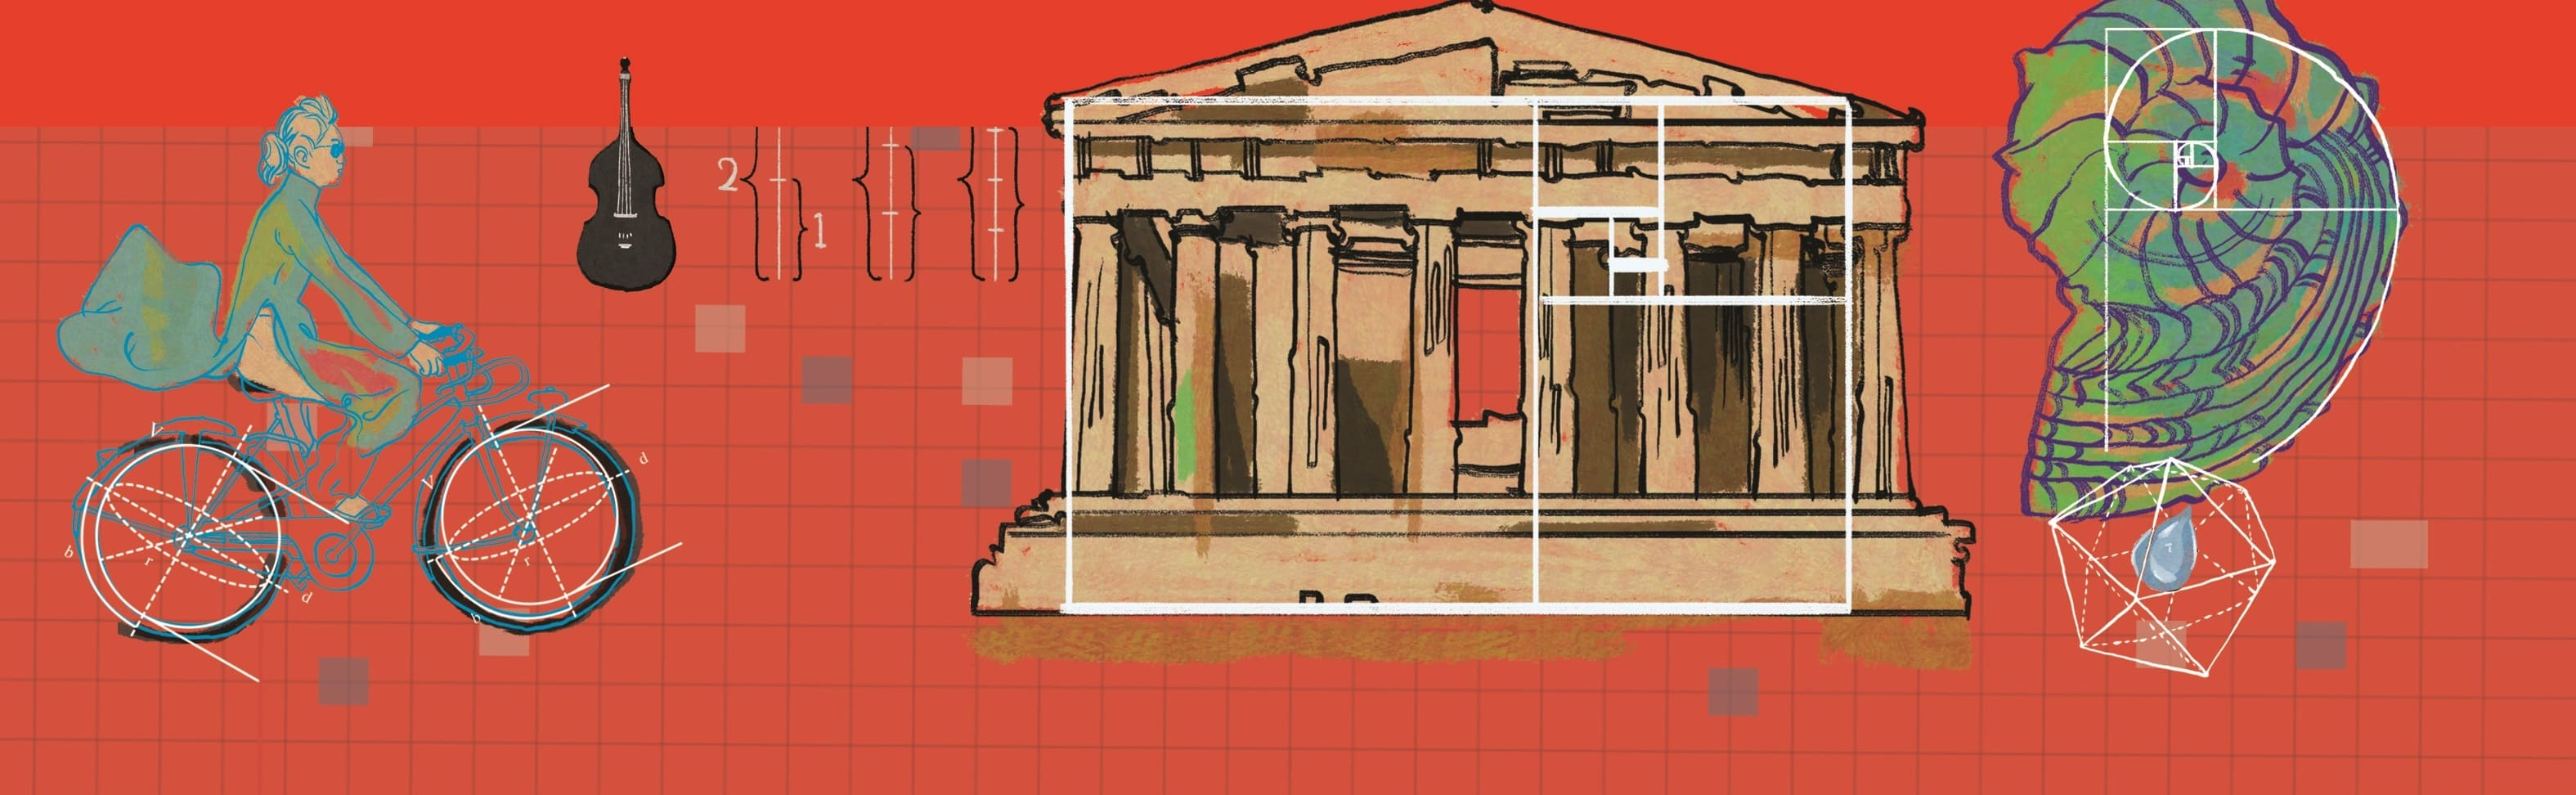
\includegraphics[width=19.3cm]{../bannertoanhocdoisong}}}
\AddToShipoutPicture*{\put(104,530){
\includegraphics[scale=1]{../tieude.pdf}}}
\centering
\endgroup

\vspace*{175pt}

\begin{multicols}{2}
	\textit{Khi các đấu thủ hoặc các đội thi đấu với nhau, cơ hội chiến thắng của mỗi bên phụ thuộc vào thực lực của họ. Hệ thống tính điểm Elo là một phương pháp tính toán trình độ tương đối của những người chơi trong một trò chơi có tổng bằng không, cho phép đánh giá khả năng về kết cục của một trận đấu.}
	\vskip 0.05cm
	Từ ngày $24$ tháng $11$ đến ngày $16$ tháng $12$ năm $2021$, tại Dubai đã diễn ra giải vô địch thế giới môn cờ vua. Kỳ thủ Nauy Magnus Carlsen, nhà vô địch từ năm $2013$, đấu với kỳ thủ Nga Ian Nepomniachtchi, người giành chiến thắng ở Giải đấu các ứng viên$^{\small{5}}$. Người chiến thắng giành được $1{,}2$ triệu euro tiền thưởng.
	\vskip 0.05cm
	Trận đấu gồm $14$ ván. Mỗi ván thắng được $1$ điểm, thua $0$ điểm và nếu hòa thì mỗi đấu thủ được $\frac{1}{2}$ điểm. Chung cuộc, Carlsen giành chiến thắng $7\frac{1}{2} - 3\frac{1}{2}$, với $4$ thắng, $0$ thua và $7$ hòa sau $11$ ván ($3$ ván cuối cùng không cần thiết vì không làm thay đổi kết quả cuối cùng). Và như vậy Carlsen giành danh hiệu vô địch thế giới lần thứ $5$ liên tiếp.
	\vskip 0.05cm
	Kết quả này phù hợp với hệ thống tính điểm Elo mà Liên đoàn Cờ vua Thế giới (FIDE) sử dụng từ năm $1970$ để đánh giá trình độ tương đối của các kỳ thủ. Quả thực, khi đó Carlsen được xếp hạng số một thế giới với số điểm Elo $2856$, trong khi đối thủ của anh, kỳ thủ số một của Nga, xếp thứ năm với số điểm Elo $2782$.
	\vskip 0.05cm
	Khi hai đấu thủ $A$ và $B$ với Elo $\theta_A$ và $\theta_B$ đấu với nhau, phương pháp Elo dự đoán $A$ sẽ giành được số điểm trung bình là
	\setlength{\abovedisplayskip}{4pt}
	\setlength{\belowdisplayskip}{5pt}
	\begin{align*}
		s_{AB} = \frac{1}{1+ 10^{-(\theta_A - \theta_B) /400}} \tag{$1$}
	\end{align*}
	biết rằng $A$ được $1$ điểm nếu thắng, $0$ nếu thua và $\frac{1}{2}$ nếu hòa. Điểm số trung bình B giành được là $s_{BA} = 1 – s_{AB}$.
	\vskip 0.05cm
	Trước trận tranh ngôi vô địch, ta có $\theta_A = 2856$ với Carlsen và $\theta_B = 2782$ với Nepomniachtchi, do đó $s_{AB} \approx 0{,}60$, tiên đoán chiến thắng của kỳ thủ Nauy vì trung bình anh sẽ giành được $8\frac{1}{2}$ điểm sau $14$ ván, so với số điểm $5\frac{1}{2}$ của kỳ thủ Nga.
	\vskip 0.05cm
	\textbf{\color{toanhocdoisong}Cơ sở toán học của phương pháp tính điểm Elo}
	\vskip 0.05cm
	Để xác định số điểm trung bình $s_{AB}$ của kỳ thủ $A$ khi đấu với kỳ thủ $B$, phương pháp ngây thơ là lấy số điểm trung bình của $A$ trong các trận đã đấu giữa hai người. Nhưng trong một trò chơi như cờ vua, phần lớn trong số hàng trăm nghìn người chơi chưa từng gặp nhau, và ngay cả khi họ đã từng gặp nhau, số trận họ đã đấu với nhau là quá ít để có một đánh giá chất lượng. Hệ thống tính điểm Elo giải quyết khó khăn này dựa vào một mô hình toán học cho phép xếp hạng các đấu thủ và qua đó ước tính kết quả có thể xảy ra khi họ đối đầu nhau.
	\vskip 0.02cm
	Biểu thức ($1$) lấy cảm hứng từ một mô hình được thiết lập từ những năm $1920$ bởi nhà toán học người Đức Ernst Zermelo và sau đó được cải tiến bởi nhà thống kê người Canada Ralph Bradley và người đồng nghiệp Milton Terry. Trong các công trình này, cũng như trong phần còn lại của bài viết, ta giả sử mọi ván đấu đều phân định thắng thua. Như vậy đây là một mô hình đơn giản hóa, nhất là đối với môn cờ vua, khi hòa là kết quả thường xảy ra nhất giữa các kỳ thủ đỉnh cao.
	\vskip 0.02cm
	Khi một ván đấu kết thúc với kết quả thắng $(1)$ hoặc thua $(0)$, điểm số trung bình chính là xác suất $p_{AB}$ để $A$ thắng $B$. Mô hình Bradley--Terry--Elo giả sử rằng xác suất này có dạng
	
	\vspace{-15pt}
	\begin{align*}
		p_{AB} = G(\theta_A - \theta_B)\tag{$2$}
	\end{align*}
	ở đó $G: \mathbb R \rightarrow (0, 1)$ là một hàm liên tục, tăng ngặt sao cho $G(x) + G(-x) = 1$ với mọi số thực $x$ và $G(x) \rightarrow 1$ khi $x \rightarrow \infty$. Một thí dụ về hàm như thế được cho trong Hình $1$. Ta có $p_{AB} + p_{BA} = G(\theta_A - \theta_B) + G(\theta_B - \theta_A) = 1$, không có kết quả hòa. Vì $G(0) = 1/2$, hai đấu thủ có trình độ ngang nhau có xác suất thắng như nhau; hiệu $\theta_A - \theta_B$ càng tăng thì xác suất để $A$ thắng càng lớn, và tiến tới giới hạn bằng $1$, nghĩa là chiến thắng chắc chắn của $A$.
	Lựa chọn phổ biến nhất của $G$ là luật logistic với tham số $\beta > 0$, được định nghĩa bởi
	
	\vspace{-15pt}
	\begin{align*}
		L(x) = \frac{ 1 }{ (1 + e^{-\beta x}) }\tag{$3$}
	\end{align*}
	với mọi $x \in \mathbb R$.
	\begin{figure}[H]
%		\vspace*{5pt}
		\centering
		\captionsetup{labelformat= empty, justification=centering}
		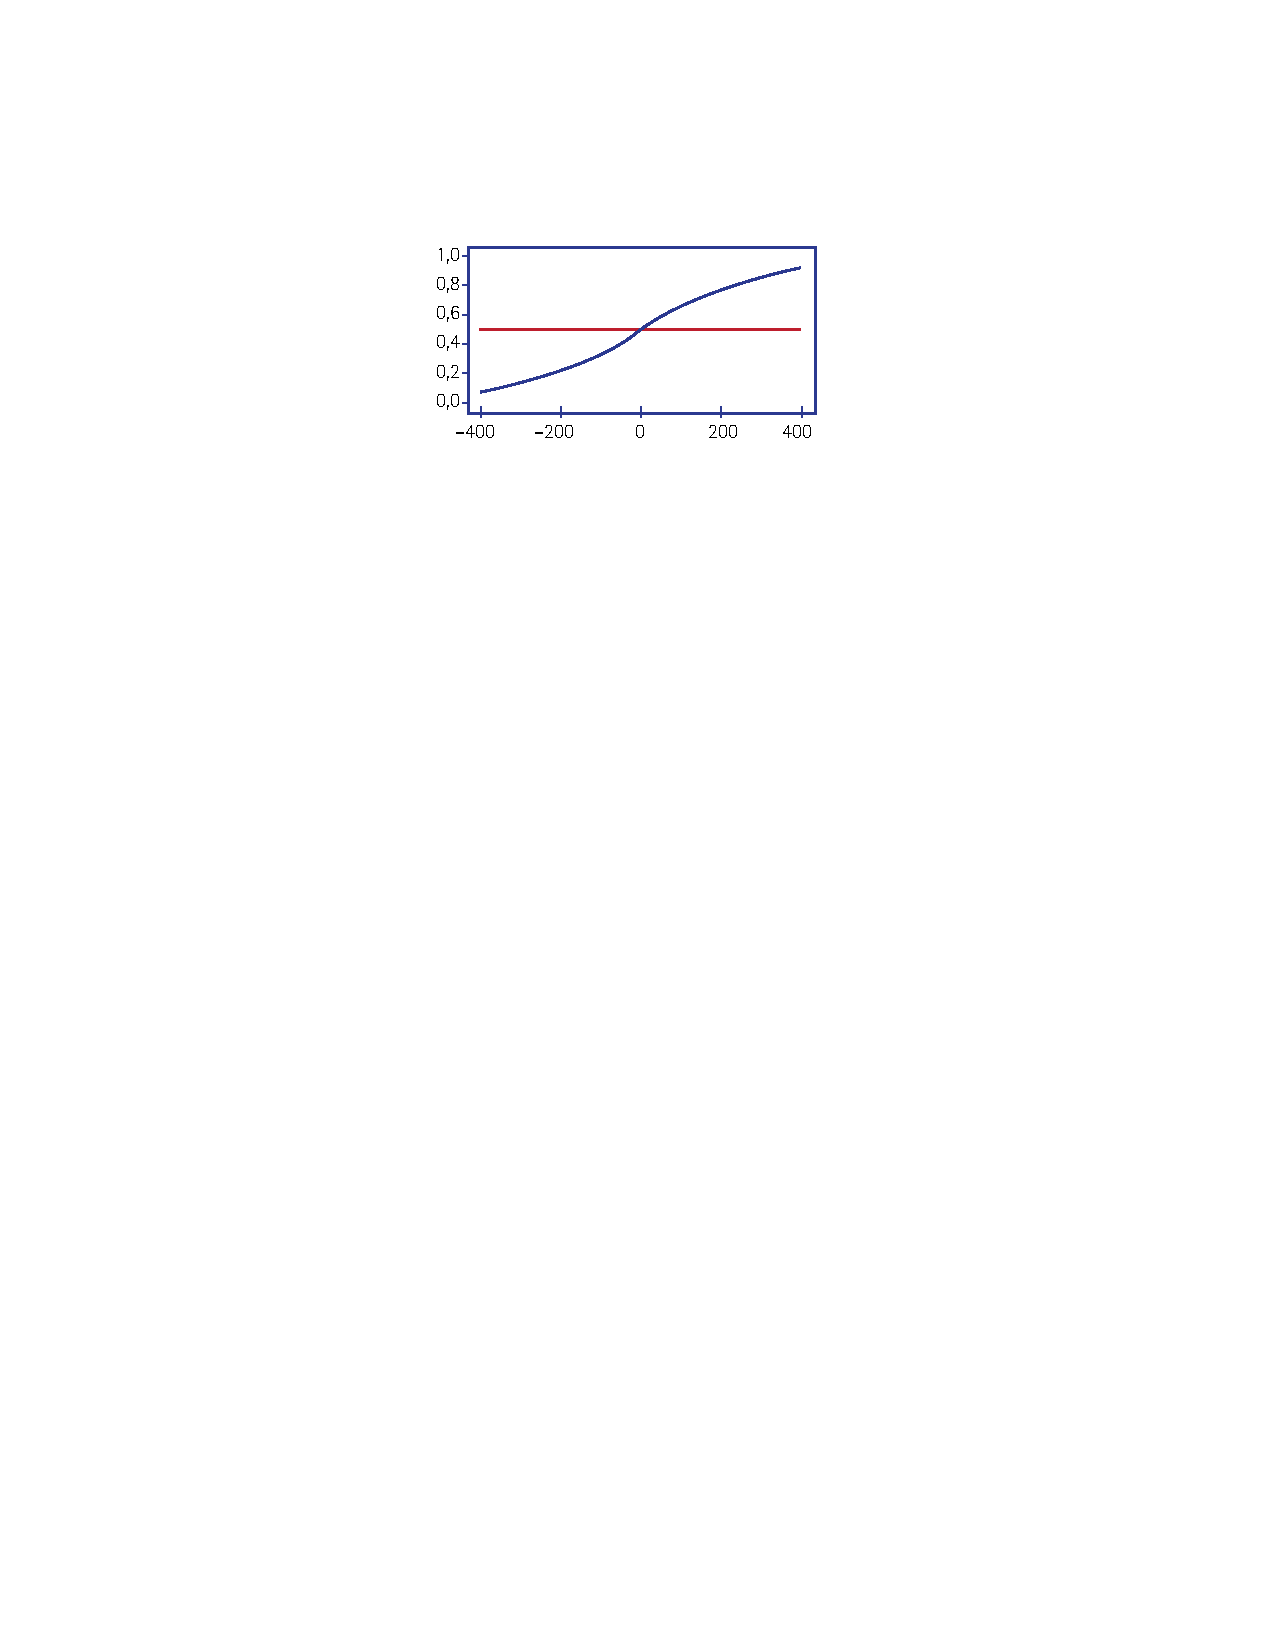
\includegraphics[width= 0.8\linewidth]{pic1}
		\caption{\small\textit{\color{toanhocdoisong}Hình $1$. Đồ thị hàm logistic $L(x)$ với $\beta = \ln(10) / 400$.}}
		\vspace*{-10pt}
	\end{figure}
	Chọn $G = L$ với tham số $\beta = \ln(10) / 400$, ta thu được công thức ($1$) mà FIDE sử dụng. Ban đầu, nhà vật lý người Mỹ gốc Hungary Arpad Elo, người đưa phương pháp mô hình hóa này vào thế giới cờ vua, sử dụng một hàm phân phối chuẩn, khi đó $s_{AB}$ không có công thức tường minh như trên.
	\vskip 0.05cm
	\textbf{\color{toanhocdoisong}Tính chất của mô hình xác suất}
	\vskip 0.05cm
	Mô hình Bradley--Terry--Elo có ưu điểm là nó cho phép xếp hạng tất cả người chơi của một trò chơi theo trình độ tương đối, ngay cả khi họ chưa từng đối đầu trực tiếp. Do đó, ta có thể dùng nó để dự đoán, đặc biệt là dựa vào các mô phỏng.
	Tuy nhiên, giả định rằng xác suất để $A$ thắng $B$ có dạng ($2$) không hề là một điều vô tình. Như đã đề cập, nó ngầm cho rằng không có ván hòa. Nếu có kết quả hòa, mô hình sẽ cần phải được điều chỉnh.
	\vskip 0.05cm
	Biểu thức ($2$) cũng ngầm giả định rằng kết quả một trận đấu giữa $A$ và $B$ chỉ phụ thuộc vào trình độ tương đối $\theta_A - \theta_B$. Đặc biệt, những yếu tố như đi trước (cầm quân trắng trong cờ vua), được nghỉ ngơi nhiều hơn đối thủ, hay thi đấu trước các cổ động viên không ảnh hưởng đến kết quả cuối cùng (một điều không hợp lý đối với thể thao chuyên nghiệp).
	\vskip 0.05cm
	Hơn nữa, cần phải hiểu rằng điểm số Elo của một đấu thủ không hề có giá trị nội tại: ý nghĩa của nó phụ thuộc vào điểm số Elo của các đối thủ, vì ta có thể cộng tất cả với cùng một hằng số tùy ý, hiệu số giữa chúng vẫn giữ nguyên. Tương tự, nếu ta nhân tất cả các Elo với một hằng số $c > 0$ và thay hàm $G(x)$ bởi $G(x / c)$, các xác suất thắng cũng không thay đổi.
	\vskip 0.05cm
	Trong trường hợp công thức ($1$), được biểu diễn trong Hình $1$ với các giá trị $\theta_A - \theta_B$ từ $-400$ đến $+400$, tham số $\beta$ được chọn sao cho chênh lệch $100$ điểm cho xác suất thắng $64\%$ đối với người mạnh hơn. Nếu chênh lệch là $200$ điểm, xác suất là $75\%$, và nó vào khoảng $91\%$ khi chênh lệch là $400$ điểm.
	\vskip 0.05cm
	Trong cờ vua, điểm Elo của hầu hết các kỳ thủ có trong xếp hạng của FIDE nằm trong khoảng từ $1000$ đến $3000$. Phân phối của chúng nói chung không đối xứng và thay đổi tùy theo từng nước. Hơn nữa, có nhiều phiên bản khác nhau của hệ thống xếp hạng, ngoài ra nó còn được điều chỉnh để áp dụng cho nhiều trò chơi và môn thể thao khác, trong đó có cờ vây, \textit{scrabble}, nhiều trò chơi trên mạng, bóng đá, tennis và khúc côn cầu trên băng.
	\vskip 0.05cm
	\textbf{\color{toanhocdoisong}Cập nhật xếp hạng}
	\vskip 0.05cm
	Tất nhiên là trình độ tương đối của các đấu thủ thay đổi theo thời gian. Một số người mạnh lên khi tích lũy thêm kinh nghiệm, một số khác yếu đi do tuổi tác, hoặc, trong trường hợp các môn thể thao đồng đội, do chấn thương, do giải nghệ hoặc do chuyển nhượng không tốt.
	\vskip 0.05cm
	Để thể hiện sự thay đổi này, phương pháp tính điểm Elo đưa ra một quy tắc cập nhật điểm xếp hạng sau mỗi trận đấu. Gọi $\theta_{A, n}$ và $\theta_{B, n}$ là điểm xếp hạng (Elo) của hai đấu thủ A và B ngay trước lần gặp nhau thứ $n$. Elo đề xuất rằng sau trận đấu này, chênh lệch $\theta_{A, n} - \theta_{B, n}$ được phân phối lại cho hai người theo ``độ bất ngờ" của kết quả và một số thực dương $k$, gọi là \textit{hệ số phát triển}.
	\vskip 0.05cm
	Gọi $s$ là kết quả của ván đấu giữa $A$ và $B$, với $s = 1$ nếu $A$ thắng, $s = 0$ nếu $A$ thua và $s = 1/2$ nếu ván đấu hòa. Elo mới của $A$ sẽ là
	\begin{align*}
		\theta_{A, n + 1} = \theta_{A, n} + k (s – s_{AB, n}),
	\end{align*}
	ở đó $s_{AB, n}$ là kết quả dự đoán được tính theo công thức ($1$) với các giá trị $\theta_{A, n}$ và $\theta_{B, n}$. Dễ thấy điểm số Elo của $A$ tăng nếu $s = 1$, và $s_{AB, n}$ càng nhỏ thì điểm số tăng càng nhiều. Như vậy, chiến thắng trước một đối thủ mạnh hơn thì có giá trị hơn. Tương tự, điểm số Elo của $A$ giảm khi thua, tức là khi $s = 0$. Cuối cùng, khi ván đấu hòa, điểm số Elo của $A$ tăng nếu điểm số Elo ban đầu của $B$ lớn hơn, tức là $s_{AB, n} < 1/2$.
	Đối với các kỳ thủ chuyên nghiệp, hệ thống tính điểm Elo cố định giá trị $k = 10$, do đó tại giải vô địch thế giới, mỗi ván thắng mang lại cho Carlsen $10 \times (1 – 0{,}60) \approx 4$ điểm Elo, trong khi mỗi ván hòa khiến anh mất $10 \times (0{,}5 – 0{,}60) \approx 1$ điểm. Sau giải đấu, điểm số Elo mới của anh là
	\begin{align*}
		2856 + 4 \times 4{,}0 - 7 \times 1{,}0 = 2865,
	\end{align*}
	trong khi đó điểm số Elo của Nepomniachtchi giảm từ $2782$ xuống $2773$.
	\vskip 0.05cm
	Các giá trị khác của $k$ được dùng cho các trình độ khác nhau của các kỳ thủ. Chẳng hạn, người ta dùng $k = 40$ cho các kỳ thủ mới chơi chưa quá $30$ ván hoặc các kỳ thủ trẻ dưới $18$ tuổi, giúp họ nhanh chóng đạt đến trình độ thực. Sau đó, $k$ được quy định bằng $20$ chừng nào điểm Elo của họ vẫn ở dưới $2400$.
	\vskip 0.05cm
	\textbf{\color{toanhocdoisong}Tính chất của phương pháp cập nhật}
	\vskip 0.05cm
	Trong trường hợp đặc biệt khi tất cả các ván đấu đều phân thắng bại, ta thấy rằng một cách tổng quát, phương pháp cập nhật mà Elo đề xuất sử dụng một hàm $M: \mathbb R \rightarrow (0, \infty)$ liên tục, giảm ngặt sao cho $M(x) \rightarrow 0$ khi $x \rightarrow \infty$. Hàm này cho phép cập nhật điểm xếp hạng của các đấu thủ $A$ và $B$ như sau.
	\vskip 0.05cm
	Nếu $A$ thắng:
	\begin{align*}
		&\theta_{A, n  +1} = \theta_{A, n} + M(\theta_{A, n} - \theta_{B, n}),\\
		&\theta_{B, n  +1} = \theta_{B, n} - M(\theta_{A, n} - \theta_{B, n}).
	\end{align*}
	Nếu $B$ thắng:
	\begin{align*}
		&\theta_{A, n  +1} = \theta_{A, n} - M(\theta_{B, n} - \theta_{A, n}),\\
		&\theta_{B, n  +1} = \theta_{B, n} + M(\theta_{B, n} - \theta_{A, n}).
	\end{align*}
	Trong công thức của FIDE, $M(x) = k L(-x)$ với mọi số thực $x$.
	\vskip 0.01cm
	Công thức cập nhật này có ý nghĩa tìm kiếm xác suất. Thực vậy, gọi $\theta_A$ và $\theta_B$ là trình độ tương đối thực sự nhưng chưa biết của hai đấu thủ $A$ và $B$. Giả sử $G(\theta_A - \theta_B)$ là xác suất thực sự để $A$ thắng $B$. Kỳ vọng của thay đổi xếp hạng của $A$ tại thời điểm $n$ được cho bởi biểu thức sau:
	\begin{align*}
		&M(\theta_{A, n} - \theta_{B, n}) G(\theta_A - \theta_B)\\
		 &- M(\theta_{B, n} - \theta_{A, n}) G(\theta_B - \theta_A).
	\end{align*}
	Nếu phương pháp cập nhật là tốt, ta mong muốn rằng kỳ vọng này bằng $0$ khi $\theta_{A, n} - \theta_{B, n} = \theta_A - \theta_B$. Do $M$ là hàm giảm, ta cũng hy vọng rằng sau ván đấu, hiệu $(\theta_{A, n + 1} - \theta_{B, n + 1}) - (\theta_A - \theta_B)$ gần $0$ hơn so với hiệu $(\theta_{A, n} - \theta_{B, n}) - (\theta_A - \theta_B)$.
	\vskip 0.01cm
	Lập luận tương tự cũng đúng đối với $B$, và ta có thể kiểm tra rằng những tính chất mong muốn này được đạt nếu các hàm $G$ và $M$ thỏa mãn, với mọi số thực $x$:
	\begin{align*}
		M(x) / M(-x) = G(-x) / G(x). \tag{$4$}
	\end{align*}
	Từ phương trình cân bằng này, với một chút nỗ lực, ta có thể chứng minh rằng với mỗi hàm $M$ cho trước, hàm $G$ duy nhất thỏa mãn được cho bởi
	\begin{align*}
		G(x) = \frac { M(-x) }{ M(x) + M(-x) },
	\end{align*}
	với mọi $x \in \mathbb R$.
	\vskip 0.01cm
	Do đó, quy tắc cập nhật mà Elo đề xuất ngầm cho rằng xác suất ban đầu là xác suất logistic, tức là $G = L$.
	\vskip 0.01cm
	Có một lưu ý tinh tế: nếu ta cố định hàm $G$ trước thì tồn tại vô số hàm $M$ thỏa mãn quan hệ ($4$). Thật vậy, với mọi hằng số $k > 0$, $M(x) = k G(-x)$ là một nghiệm. Nhưng ta cũng có thể chọn $M(x) = k G(-x) S(|x|)$, ở đó $S$ là một hàm thỏa mãn $S(0) = 1$ và $S(x) = S(-x)$ với mọi số thực $x$. Tất nhiên là hàm $S$ được chọn phải đảm bảo tính đơn điệu giảm của $M$.
	\vskip 0.05cm
	\textbf{\color{toanhocdoisong}Kết quả về sự hội tụ}
	\vskip 0.05cm
	Có thể liên hệ phương pháp cập nhật của Elo với thuật toán giảm gradient ngẫu nhiên trong học máy trong một mô hình hồi quy logistic.
	\vskip 0.05cm
	Ta hãy tưởng tượng có $N$ đấu thủ và trình độ của họ được biểu diễn bởi vector $(\theta_1, \dots, \theta_N)$ ẩn nhưng cố định. Ta cũng giả sử rằng ban đầu, ta có một ước lượng $(\theta_{1, 0}, \dots, \theta_{N, 0})$, và các đấu thủ sẽ tham gia một dãy vô hạn các ván đấu, mỗi ván diễn ra 
	\end{multicols}
	\vspace*{-8pt}
	\begin{tBox}
		\begin{wrapfigure}{l}{0.18\linewidth}
			\vspace*{-15pt}
			\centering
			\captionsetup{labelformat= empty, justification=centering}
			\hspace*{3pt}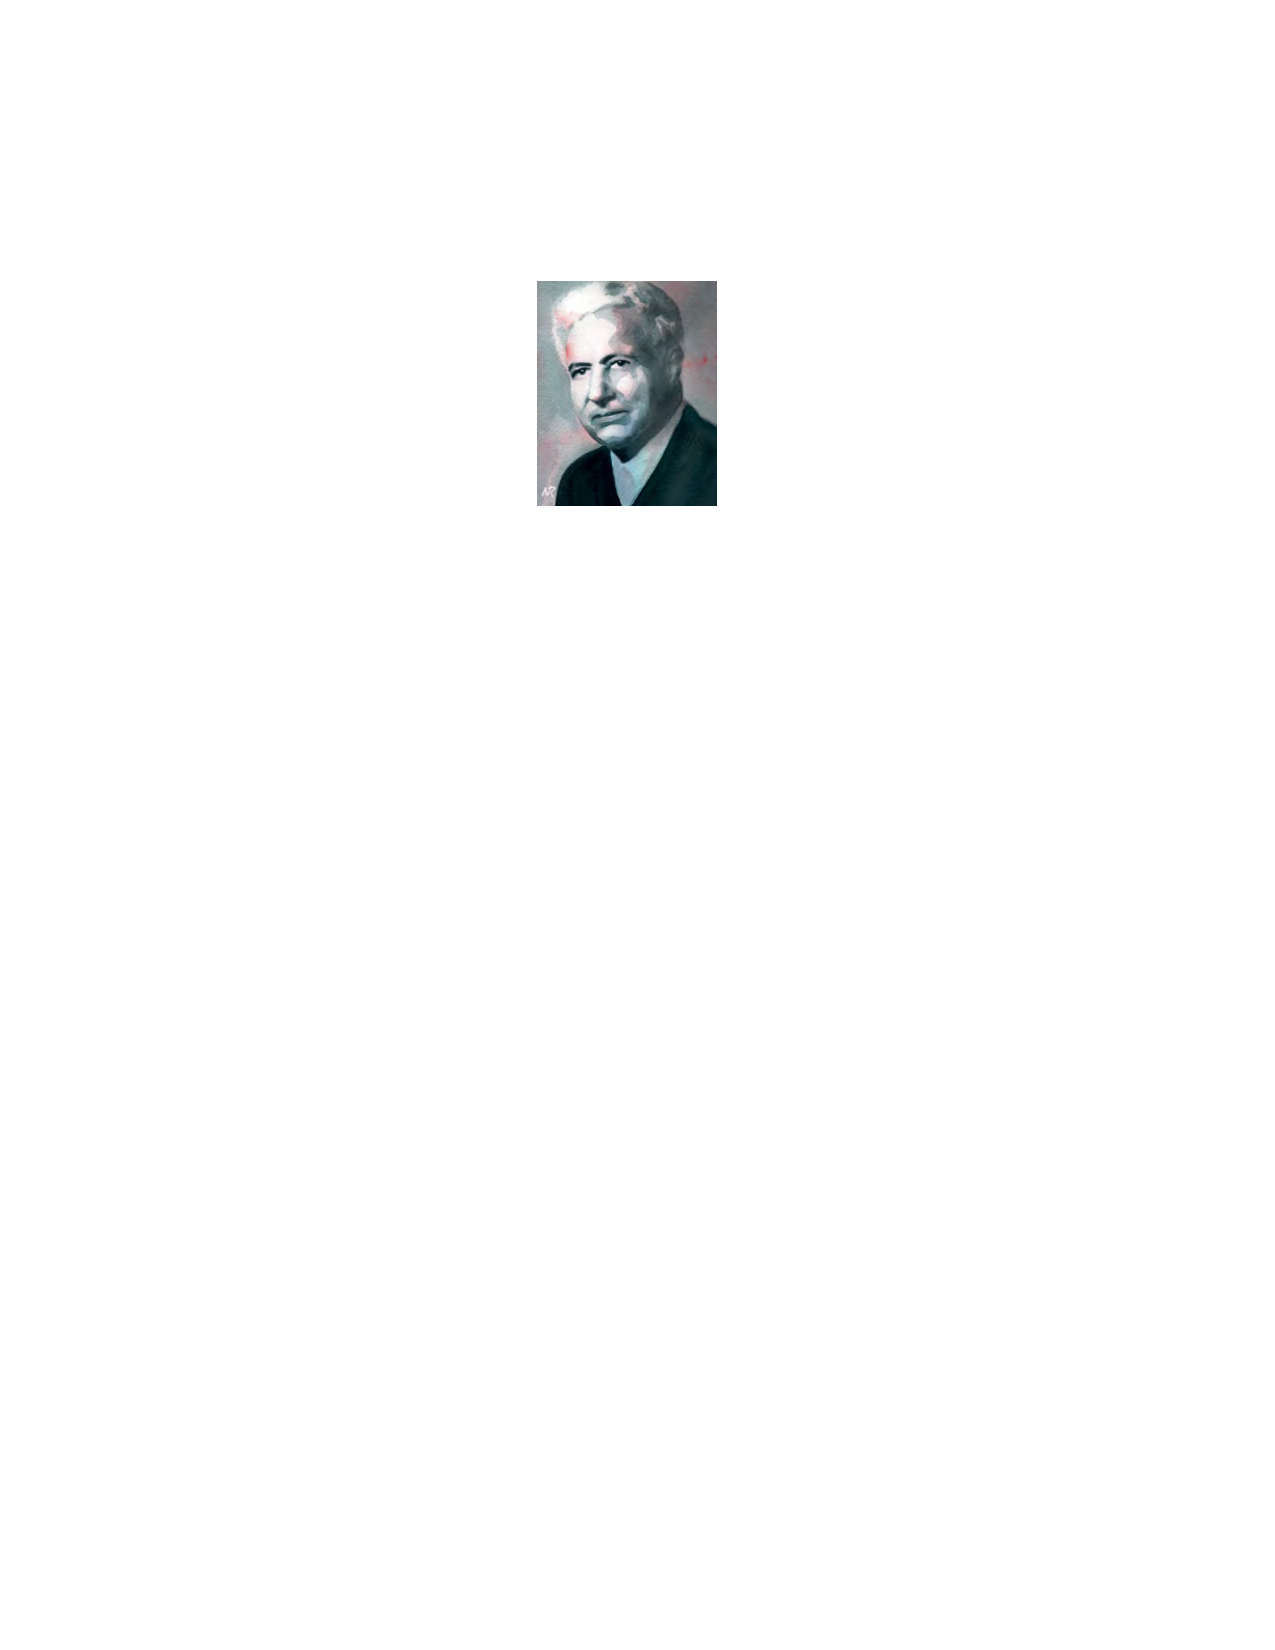
\includegraphics[width= 1.1\linewidth]{pic2}
			\caption{\small\textit{\color{toanhocdoisong}\hspace*{15pt}Arpad Elo.}}
			\vspace*{-20pt}
		\end{wrapfigure}
		Sinh ngày $25$ tháng $8$ năm $1903$ tại Egyházaskeszö, Áo--Hung trong một gia đình khiêm tốn, Arpad Elo (Élö Árpád trong tiếng Hungary) di cư sang Mỹ năm $1913$ cùng cha mẹ. Ông học vật lý tại Đại học Chicago, sau đó giảng dạy tại Đại học Marquette Milwaukee, Wisconsin.
		\vskip 0.05cm
		Ông là một kỳ thủ tài ba, từng tám lần vô địch bang và là chủ tịch Liên đoàn Cờ vua Mỹ từ $1935$ đến $1937$. Ông nổi tiếng thế giới vì đã đưa vào sử dụng hệ thống mang tên mình, được xây dựng trong những năm $1950$ sau khi hệ thống xếp hạng đầu tiên, do Kenneth Harkness phát triển, bị chỉ ra những nhược điểm. Phương pháp mới được FIDE thông qua vào năm $1970$, và Elo trở thành thành viên danh dự của tổ chức này từ năm $1981$.
		\vskip 0.05cm
		Một phân tích chi tiết đầu tiên về hệ thống tính điểm Elo (có khi bị viết sai thành ELO như thể một từ viết tắt) được chính Elo đưa ra trong cuốn sách năm $1978$ của mình, The Rating of Chessplayers, Past and Present. Ngày nay, phương pháp của ông là một phần không thể tách rời của thế giới cờ vua. Nó được dùng để xác định cách các kỳ thủ đối đầu với nhau tại các giải cờ vua trên toàn thế giới, và mọi kỳ thủ đều theo dõi sát sao sự thay đổi điểm số Elo của mình để đo mức độ tiến bộ và biết được thứ bậc của mình trong cờ vua.
		\vskip 0.05cm
		Arpad Elo qua đời ngày $5$ tháng $11$ năm $1992$ (thọ $89$ tuổi) tại Brookfield, Wisconsin.
		\vspace*{-3pt}
	\end{tBox}
	\begin{multicols}{2}
	giữa hai đấu thủ được chọn ngẫu nhiên theo phân phối đều. Cuối cùng, tưởng tượng rằng sau mỗi ván, vector trình độ được cập nhật theo phương pháp của Elo tại hai tọa độ $i$ và $j$ của hai đấu thủ vừa thi đấu.
	\vskip 0.05cm
	Dưới giả thiết các hàm $G$ và $M$ thỏa mãn các điều kiện đã nói đến ở trên, và hơn nữa $M$ có đạo hàm bị chặn, nhà toán học người Anh David Aldous đã chứng minh được rằng khi $n$ tiến ra vô cùng, dãy các vector $(\theta_{1, n}, \dots, \theta_{N, n})$ đạt đến một phân phối dừng. Liệu phân phối dừng này có phải là một xấp xỉ tốt của $(\theta_1, \dots, \theta_N)$ hay không vẫn là một câu hỏi lý thuyết mở, mặc dù nó đã được khẳng định bởi nhiều mô phỏng và thực tế hàng chục năm sử dụng hệ thống xếp hạng Elo của các kỳ thủ cờ vua.
	\vskip 0.05cm
	Trong khi đó, mặc dù kết quả hội tụ như của Aldous tạo niềm tin đối với phương pháp của Elo, chưa chắc đã tồn tại một vector ẩn $(\theta_1, \dots, \theta_N)$ phản ánh trình độ thực sự của các đấu thủ. Rốt cuộc thì các đấu thủ thay đổi theo thời gian, và các đội thể thao cũng liên tục thay đổi. Vector trình độ thực, nếu tồn tại, là một vector động.
	\vskip 0.05cm
	Thành công của phương pháp tính điểm Elo nằm ở khả năng theo được sự thay đổi này mà không phải phụ thuộc vào một mô hình ngẫu nhiên chính xác. Đây là một thực tế được xác nhận trong môn cờ vua, và trong cả nhiều tình huống khác, trong đó tham số $\beta$ và hệ số phát triển $k$ cần được lựa chọn một cách thích hợp.
	\vskip 0.05cm
	\textbf{\color{toanhocdoisong}Hệ thống Elo trong khúc côn cầu}
	\vskip 0.05cm
	Để minh họa phương pháp tính điểm Elo và khả năng dự đoán của nó ở ngoài môn cờ vua, ta hãy cùng xem xét ứng dụng của nó trong môn khúc côn cầu trên băng\footnote[6]{\color{toanhocdoisong}Accromath là tạp chí Canada, nơi khúc côn cầu trên băng là môn thể thao phổ biến nhất -- Pi.}, trong đó nhiều điều chỉnh đã được thực hiện để tận dụng kết quả của tất cả các trận trong vòng đấu thường và vòng đấu loại trực tiếp của giải National Hockey League (NHL) kể từ khi nó ra đời vào năm $1917$. Các dữ liệu này được lưu tại trang \url{hockey-reference.com}.
	\vskip 0.05cm
	Thí dụ, các nhà phân tích Ryan Best và Neil Paine của trang \textit{FiveThirtyEight} đề xuất một hệ thống xếp hạng Elo tính đến các tham số sau:
	\vskip 0.05cm
	$a)$ Mỗi đội có số diểm Elo ban đầu là $1380$.
	\vskip 0.05cm
	$b)$ Quy tắc cập nhật sử dụng hệ số phát triển $k = 6$.
	\vskip 0.05cm
	$c)$ Ta tính đến lợi thế sân nhà, tức là nếu hai đội có cùng Elo, đội chủ nhà có xác suất thắng là $57{,}1\%$ thay vì $50\%$.
	\vskip 0.05cm
	$d)$ Thay đổi điểm Elo tăng thêm $25\%$ đối với những trận loại trực tiếp.
	\vskip 0.05cm
	$e)$ Đầu mỗi mùa giải, điểm Elo của mỗi đội được tính lại, bằng
	\begin{align*}
		0{,}7 \!\times\!\text{điểm xếp hạng mùa trước} + 0{,}3 \!\times\!\! 1505.
	\end{align*}
	Như vậy, điểm số Elo trung bình của cả mùa giải dao động hàng năm xung quanh $1500$.
	\begin{figure}[H]
		\vspace*{-5pt}
		\centering
		\captionsetup{labelformat= empty, justification=centering}
		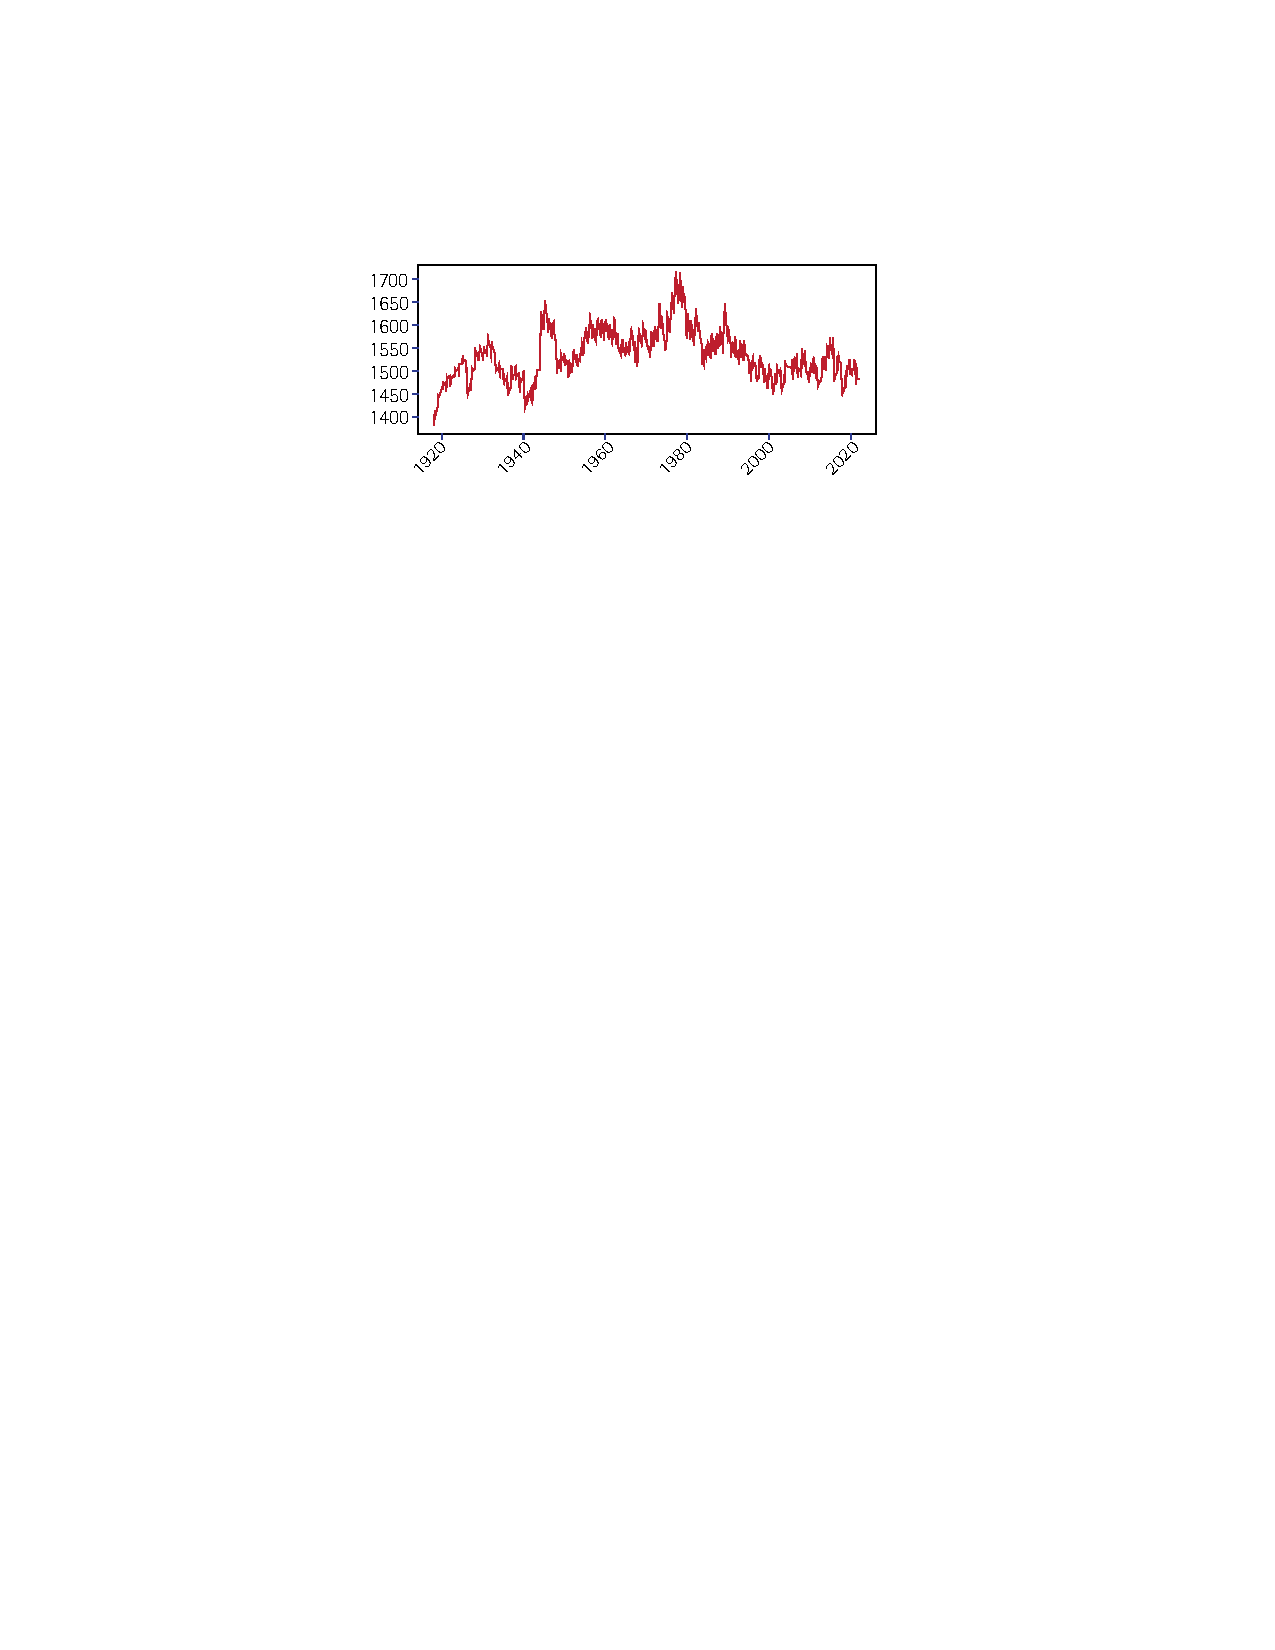
\includegraphics[width= 1\linewidth]{pic3}
		\caption{\small\textit{\color{toanhocdoisong}Hình $2$. Xếp hạng Elo của đội Montreal Canadiens từ năm $1917$ đến nay.}}
		\vspace*{-10pt}
	\end{figure}
	Ngoài ra, mô hình của Best và Paine tính đến cả hiệu số bàn thắng -- bàn thua của mỗi trận đấu và sự phụ thuộc lẫn nhau (hay tự tương quan) giữa các trận đấu liên tiếp.
	\vskip 0.05cm
	Hình $2$ cho thấy sự thay đổi của xếp hạng Elo của đội Montreal Canadiens theo mô hình của Best và Paine. Đỉnh cao nhất của đồ thị nằm ở nửa sau của thập niên $1970$, giai đoạn mà họ giành được bốn cúp Stanley\footnote[7]{\color{toanhocdoisong}Danh hiệu vô địch hàng năm của NHL -- Pi.}  liên tiếp.
	\vskip 0.05cm
	Ta cũng có thể thấy các đỉnh khác trong nửa sau thập niên $1940$ và giữa những năm $1990$, cũng như thời kỳ xuất sắc ổn định cuối những năm $1950$, khi họ vô địch năm lần liên tiếp (từ $1956$ đến $1960$). Trái lại, xếp hạng Elo của đội dao động quanh mức trung bình kể từ đầu những năm $2000$. Sự hiện diện của họ tại trận chung kết cúp Stanley năm $2021$, bởi vậy, có ít khả năng lặp lại trong tương lai gần.
	\vskip 0.05cm
	Vì xếp hạng Elo có tính tương đối, sẽ bổ ích hơn nếu ta so sánh sự thay đổi xếp hạng của các câu lạc bộ khác nhau. Hình $3$ so sánh các đội Montreal Canadiens (đường màu đỏ), Toronto Maple Leafs (xanh nước biển) và năm đội giành cúp Stanley từ $2008$ đến $2017$, gồm Boston Bruins (da cam), Detroit Red Wings (xanh lá cây), Chicago Blackhawks (đen), Los Angeles Kings (tím) và Pittsburgh Penguins (vàng).
	\begin{figure}[H]
		\vspace*{-10pt}
		\centering
		\captionsetup{labelformat= empty, justification=centering}
		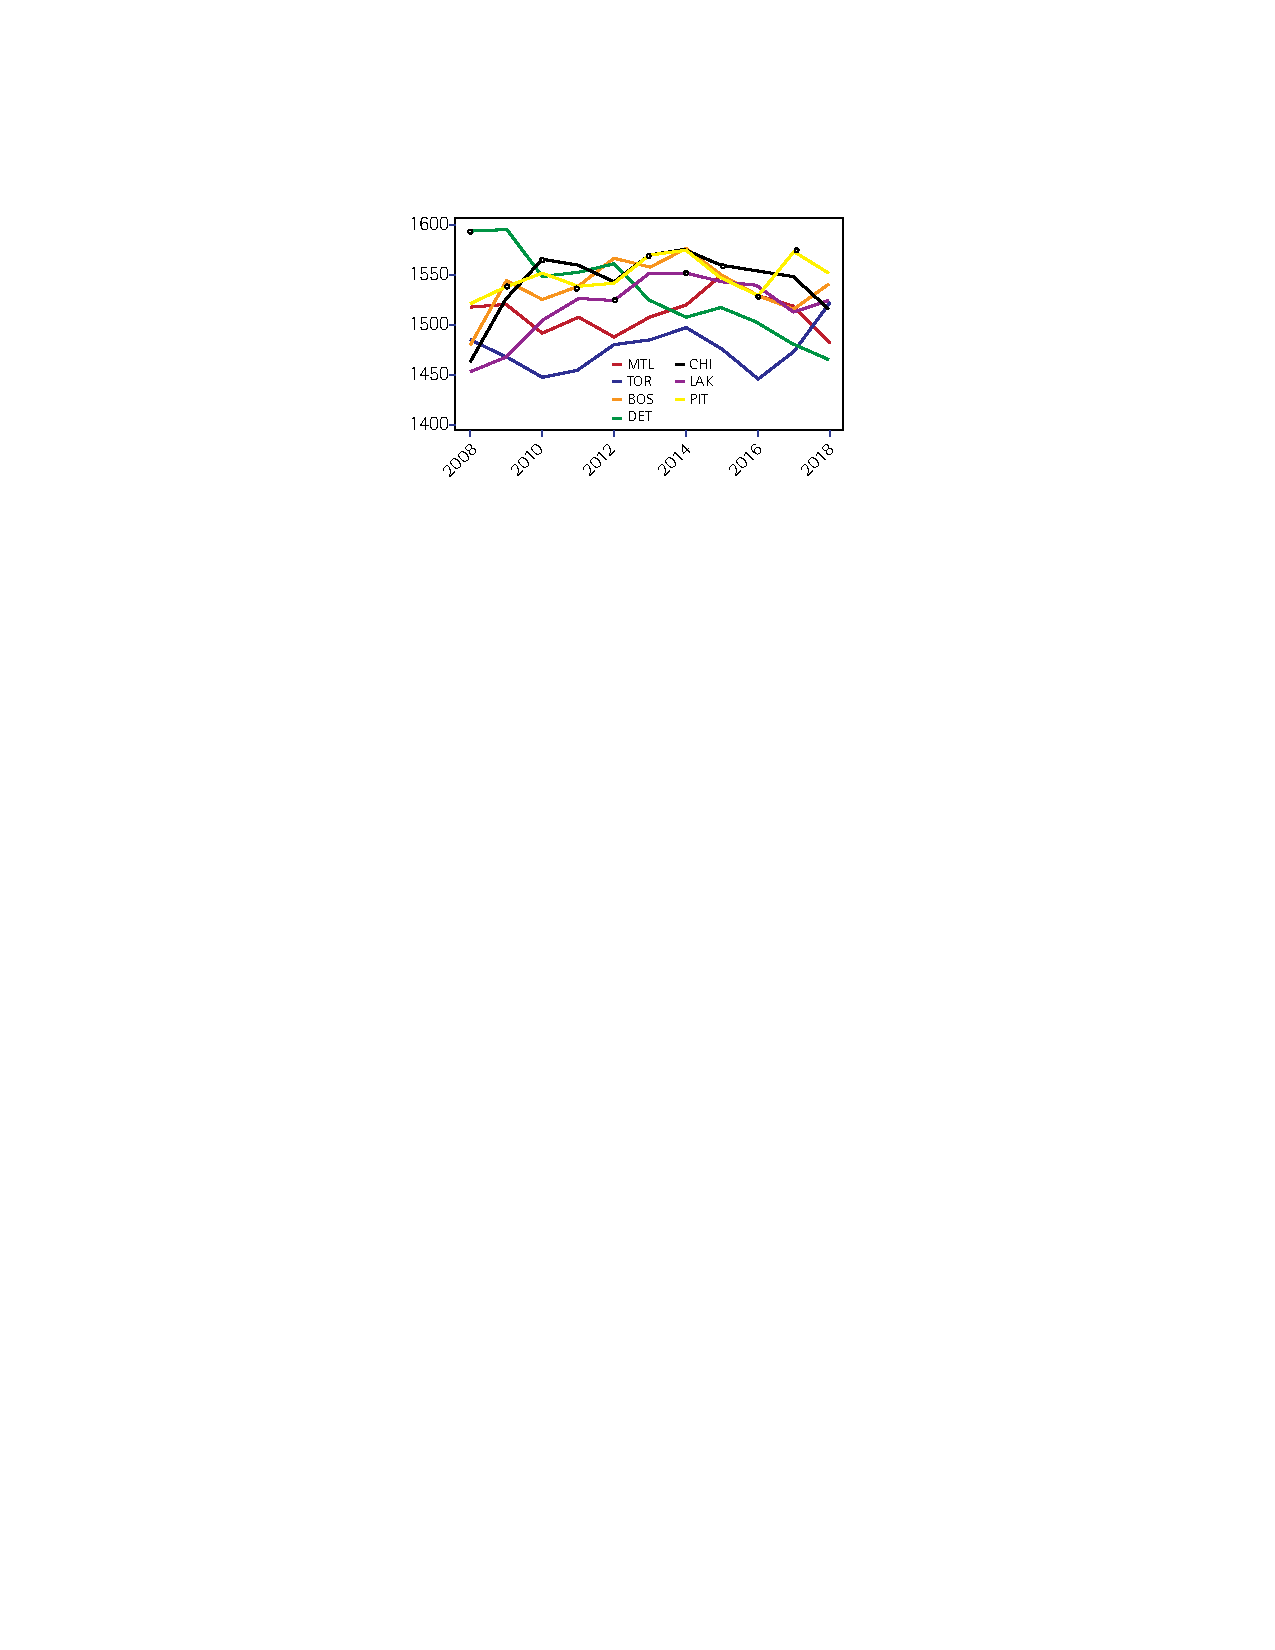
\includegraphics[width= 1\linewidth]{pic4}
		\caption{\small\textit{\color{toanhocdoisong}Hình $3$. Xếp hạng Elo của bảy đội NHL từ $2008$ đến $2018$; đội vô địch mỗi năm từ $2008$ đến $2017$ được đánh dấu bằng hình tròn.}}
		\vspace*{-10pt}
	\end{figure}
	Trong Hình $3$, các đội vô địch được đánh dấu bằng hình tròn. Đội vô địch năm $2018$, Washington Capitals, không được xét đến trong hình. Có thể thấy rõ là đội hay nhất không phải lúc nào cũng vô địch.
	\vskip 0.05cm
	\textbf{\color{toanhocdoisong}Kết luận}
	\vskip 0.05cm
	Là một yếu tố không thể thiếu trong thế giới cờ vua đồng thời có thể được áp dụng cho các trò chơi hai người có tổng bằng không nói chung, hệ thống tính điểm Elo cho phép đánh giá trình độ tương đối của các đấu thủ ngay cả khi họ chưa từng đối đầu nhau. Sự cập nhật liên tục dần dần qua từng trận đấu đem lại một cách đơn giản và hiệu quả để nắm bắt quá trình thay đổi của các đấu thủ hoặc của các đội, như được minh họa trong thí dụ về NHL.
	\vskip 0.05cm
	\PIbox{\textbf{\color{toanhocdoisong}Xếp hạng Elo của các kỳ thủ cờ vua}
		\vskip 0.05cm
		Ngày nay, một người mới chơi có điểm số Elo khoảng $1000$, còn một người chơi nghiệp dư giỏi có điểm số Elo khoảng $2000$. Các đại kiện tướng quốc tế cần đạt được điểm số Elo tối thiểu $2500$. Nhóm này gần như trùng với nhóm các kỳ thủ chuyên nghiệp, ngày nay có hơn $1000$ người trên toàn thế giới. Cho đến nay chỉ có khoảng mười lăm kỳ thủ từng đạt đến mức điểm Elo $2800$ trong sự nghiệp của mình.
		\vskip 0.05cm
		Các phần mềm cờ vua cũng có xếp hạng điểm Elo. Chương trình tốt nhất hiện nay, Stockfish, có điểm số Elo khoảng $3700$, cho thấy trong cờ vua máy tính đã vượt xa con người như thế nào: xác suất $p_{AB}$ giữa Stockfish ($A$) và Magnus Carlsen ($B$) là khoảng $0{,}992\ldots$ (tức là trung bình $992$ trận thắng và $8$ trận thua cho máy tính sau $1000$ trận đấu không có hòa). Đó cũng là khoảng cách giữa Carlsen và một kỳ thủ nghiệp dư giỏi có điểm số Elo $2000$, mức đạt được bởi khoảng $30000$ người.
		\vskip 0.05cm
		Ta cũng có thể đặt câu hỏi liệu xếp hạng Elo có thể g  iúp so sánh các kỳ thủ thuộc các thời đại khác nhau. Chẳng hạn, một kỳ thủ có điểm Elo $2700$ trong thập niên $1980$ liệu có trình độ tương đương với một kỳ thủ có điểm Elo $2700$ ngày nay? Đây là một câu hỏi phức tạp, nhất là khi bản thân môn cờ vua cũng đã thay đổi. Chẳng hạn, các kỳ thủ, từ những người chuyên nghiệp đến những người nghiệp dư hăng hái nhất, đều dùng phần mềm để luyện tập. Nhưng người ta cũng quan sát được hiện tượng ``lạm phát", được gây ra bởi chính cách tính điểm Elo. Từ đầu những năm $2000$, điểm Elo trung bình của $50$ kỳ thủ mạnh nhất đã tăng hàng chục điểm, do đó điểm Elo cỡ $2700$ ở năm $2010$ rất có thể kém giá trị hơn so với ở năm $2000$.}
\end{multicols}
%	\newpage

%	\setcounter{figure}{0}
%	\thispagestyle{quantoannone}
\pagestyle{quantoan}
\everymath{\color{quantoan}}
\graphicspath{{../quantoan/pic/}}
\blfootnote{\color{quantoan}\color{quantoan}$^1$Viện Toán học.}
\begingroup
\AddToShipoutPicture*{\put(0,616){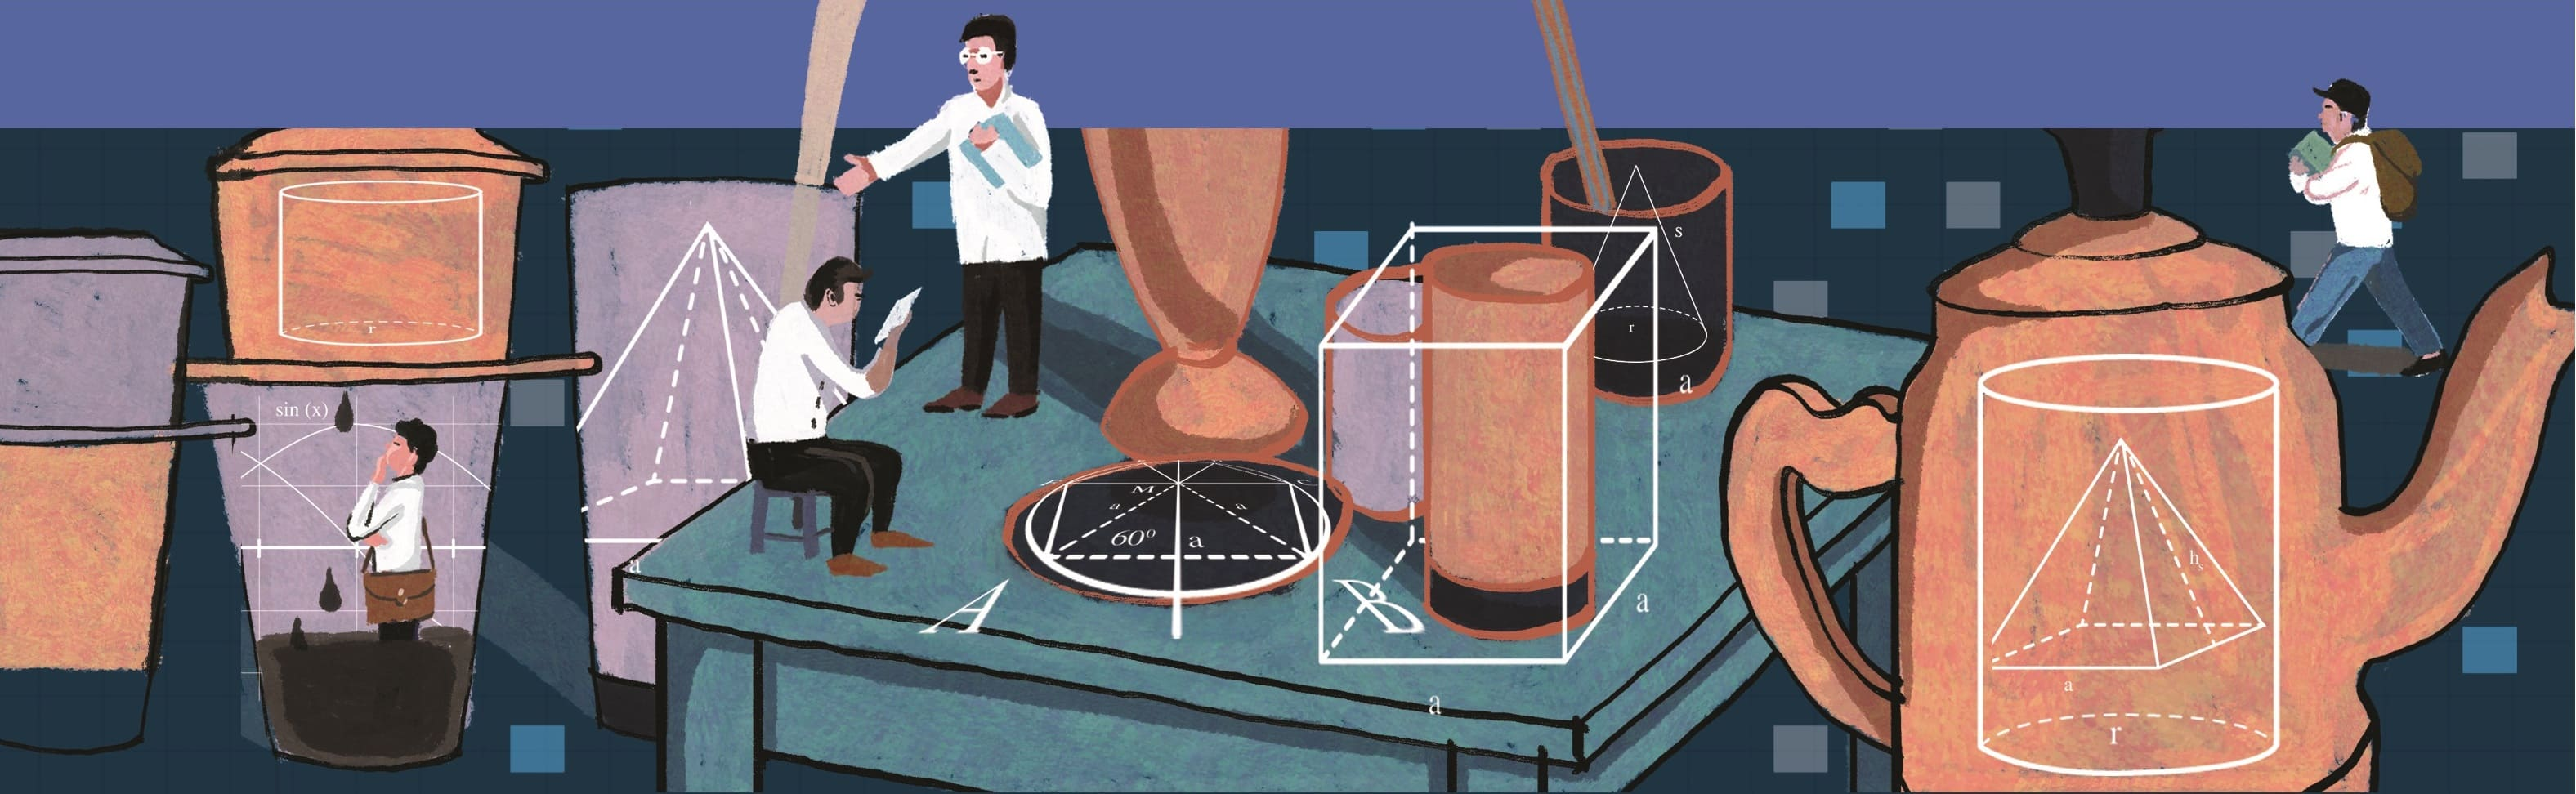
\includegraphics[width=19.3cm]{../bannerquantoan}}}
\AddToShipoutPicture*{\put(156,550){
\includegraphics[scale=1]{../tieude.pdf}}}
\centering
\endgroup

\vspace*{160pt}

\begin{multicols}{2}	
	Ngày nay số âm đã được học sinh làm quen từ lớp $6$. Nhưng nhân loại đã mất tới $2000$ năm để có thể chấp nhận được nó như cách mà học sinh lớp $6$ ngày nay chấp nhận. 
	\begin{figure}[H]
		\vspace*{-5pt}
		\centering
		\captionsetup{labelformat= empty, justification=centering}
		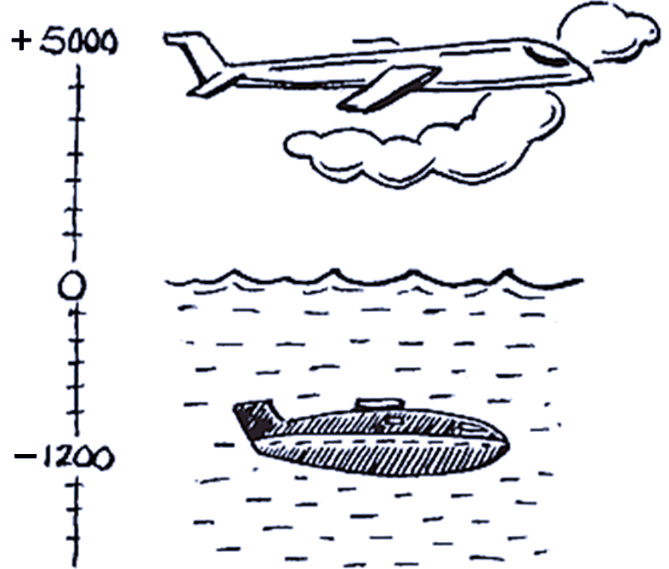
\includegraphics[width= 1\linewidth]{1}
%		\caption{\small\textit{\color{}}}
		\vspace*{-10pt}
	\end{figure}
	Nhìn lại lịch sử cho chúng ta thấy sự vật lộn trong quá trình trừu tượng hóa của Toán học. Hy vọng, theo dõi quá trình vất vả này, các thầy cô giáo THCS sẽ có thêm sự cảm thông đối với những học sinh ``dốt toán". Biết đâu, các em có thể không dốt mà chỉ đang vật lộn với việc phản biện như những nhà toán học kiệt xuất đã từng phản biện về số âm? 
	\vskip 0.1cm
	-- Thế kỷ V TCN, Hy Lạp: Trường phái Pythagoras coi số là ``nhiều đơn vị". Vì vậy với họ ``một" không phải là một số. Không có dấu hiệu nào về số âm trong các ghi chép của họ.
	\vskip 0.1cm
	-- Thế kỷ IV TCN, Hy Lạp: Aristotle đã đưa ra sự phân biệt giữa số (tức là số tự nhiên) và độ lớn (``số đó chia hết thành các số chia mà có thể chia vô hạn"), nhưng không đưa ra dấu hiệu nào về khái niệm số âm hoặc độ lớn âm.
	\vskip 0.1cm
	-- Khoảng năm $300$ TCN, Hy Lạp: Các tập VII, VIII và IX trong cuốn \textit{Cơ sở} của Euclid liên quan đến lý thuyết cơ bản về số. Euclid tiếp tục sự phân biệt của Aristotle giữa số và độ lớn, nhưng vẫn không có dấu hiệu nào về số âm.
	\vskip 0.1cm
	-- Thế kỷ I TCN -- thế kỷ I, Trung Quốc: Trong \textit{Cửu chương Toán thuật}, số âm đã được sử dụng trong chương về giải hệ phương trình. Các que màu đỏ được sử dụng để biểu thị các hệ số dương, màu đen để biểu thị các hệ số âm. Các quy tắc cho số có dấu đã được đưa ra.
	\vskip 0.1cm
	-- Thế kỷ III, Hy Lạp: Dấu hiệu đầu tiên về số âm trong một tác phẩm phương Tây xuất hiện trong cuốn \textit{Số học} của Diophantus, trong đó ông gọi phương trình mà trong ký hiệu hiện đại sẽ được biểu thị bởi $4x + 20 = 0$ là ``vô lý", vì nó sẽ cho nghiệm $x=-4$. Ông cũng nói, ``một số bị trừ, nhân với một số bị trừ, cho một số được cộng (thêm vào)". Vì vậy ông có thể xử lý các biểu thức chẳng hạn như $(x–1)(x-2)$, trong ký hiệu hiện đại. Tuy nhiên, có thể tìm thấy những chỉ dẫn trong tác phẩm của Diophantus rằng ông không có khái niệm trừu tượng về số âm.
	\vskip 0.1cm
	-- Thế kỷ VII, Ấn Độ: Số âm được sử dụng để biểu thị các khoản nợ trong khi số dương biểu thị tài sản. Nhà toán học và thiên văn học Brahmagupta đã sử dụng các số âm để thống nhất phương pháp xử lý phương trình bậc hai của Diophantus từ ba trường hợp thành một trường hợp duy nhất mà chúng ta quen thuộc ngày nay.
	\vskip 0.1cm
	-- Thế kỷ IX, Trung Đông: Mặc dù người Ả Rập đã quen thuộc với các số âm từ công trình của các nhà toán học Ấn Độ, nhưng họ bác bỏ chúng. Cuốn sách \textit{al--Kitāb al--Mukhtaṣar fī Ḥisāb al--Jabr wal--Muqābalah} (mà từ đó chúng ta có thuật ngữ ``algebra" -- đại số) của Muhammad ibn Musa al-Khwarizmi không sử dụng số âm hoặc hệ số âm.
	\vskip 0.1cm
	-- Thế kỷ XIII, Trung Quốc: Các số âm được biểu thị bằng cách vẽ một nét chéo qua chữ số khác không ngoài cùng bên phải của số đó.
	\vskip 0.1cm
	-- Thế kỷ XIII, Châu Âu: Fibonacci không đề cập đến số âm trong cuốn sách \textit{Liber Abaci} của mình, nhưng trong cuốn \textit{Flos} sau đó, ông giải thích nghiệm âm như là sự thua lỗ.
	\vskip 0.1cm
	-- Thế kỷ XV, Châu Âu: Chuquet là người đầu tiên sử dụng số âm trong một tác phẩm ở Châu Âu.
	\vskip 0.1cm
	-- Thế kỷ XVI, Châu Âu: 
	\vskip 0.1cm
	$\circ$ Cardan (Cardano), trong cuốn sách \textit{Ars Magna} của mình đã đưa vào các nghiệm âm của các phương trình và nêu các quy luật cơ bản của hoạt động với các số âm. Ông gọi các số dương là thực và các số âm là hư cấu.
	\vskip 0.1cm
	$\circ$ Viete không thừa nhận số âm.
	\vskip 0.1cm
	-- Thế kỷ XVII, Châu Âu:
	\vskip 0.1cm
	$\circ$ Descartes chấp nhận một phần khái niệm số âm. Ông không công nhận nghiệm âm vì chúng đại diện cho các số ``nhỏ hơn không có gì". Tuy nhiên, ông đã chỉ ra rằng một phương trình có nghiệm âm có thể được biến đổi thành một phương trình có nghiệm dương, điều này khiến ông chấp nhận các số âm.
	\vskip 0.1cm
	$\circ$ Pascal coi phép ``trừ đi $4$ từ 0" là điều hoàn toàn vô nghĩa.
	\vskip 0.1cm
	$\circ$ Nhà thần học và toán học Antoine Arnauld lập luận chống lại số âm bằng cách sử dụng tỷ lệ; nói rằng tỷ lệ $-1$ trên $1$ giống với tỷ lệ $1$ trên $-1$ là vô lý, vì ``Làm thế nào tỷ lệ giữa một anh nhỏ với một anh lớn hơn lại như giữa anh lớn hơn với anh nhỏ hơn?"
	\vskip 0.1cm
	-- Thế kỷ XVIII, Châu Âu:
	\vskip 0.1cm
	$\circ$ Leibniz đồng ý với lập luận của Arnaud đối với các số âm, nhưng nói rằng vì về hình thức các tỷ lệ như vậy là đúng, nên người ta vẫn có thể tính toán với chúng.
	\vskip 0.1cm
	$\circ$ Maclaurin đã xử lý các đại lượng âm ngang hàng với các đại lượng dương trong tác phẩm \textit{A Treatise of Algebra} của ông.
	\vskip 0.1cm 
	$\circ$ Euler mở đầu tác phẩm \textit{Nhập môn tổng quan về Đại số} với một thảo luận về các phép toán trên các đại lượng dương và âm. Ông sử dụng ví dụ về một khoản nợ để biện minh rằng một số âm lần số dương là một số âm.  
	\vskip 0.1cm
	-- Thế kỷ XIX, Châu Âu: Hamilton đã cố gắng đưa các số âm lên một nền tảng lý thuyết vững chắc (thay vì khái niệm về đại lượng ``nhỏ hơn không có gì") bằng cách sử dụng ý tưởng về ``thời gian thuần túy" xuất phát từ tác phẩm \textit{Phê bình lý tính thuần túy} của Kant. Nỗ lực này có vẻ khá kỳ lạ đối với chúng ta ngày nay, nhưng nó đã giúp ích trong việc phát triển các \textit{quaternion}, ví dụ đầu tiên về một hệ đại số không thỏa mãn tính giao hoán.
	\begin{flushright}
		Theo \url{https://web.ma.utexas.edu/users/mks/326K/Negnos.html}
	\end{flushright}
\end{multicols}
%	\newpage
%
%	\thispagestyle{empty}
%	\begingroup 
%	\AddToShipoutPicture*{\put(0,0){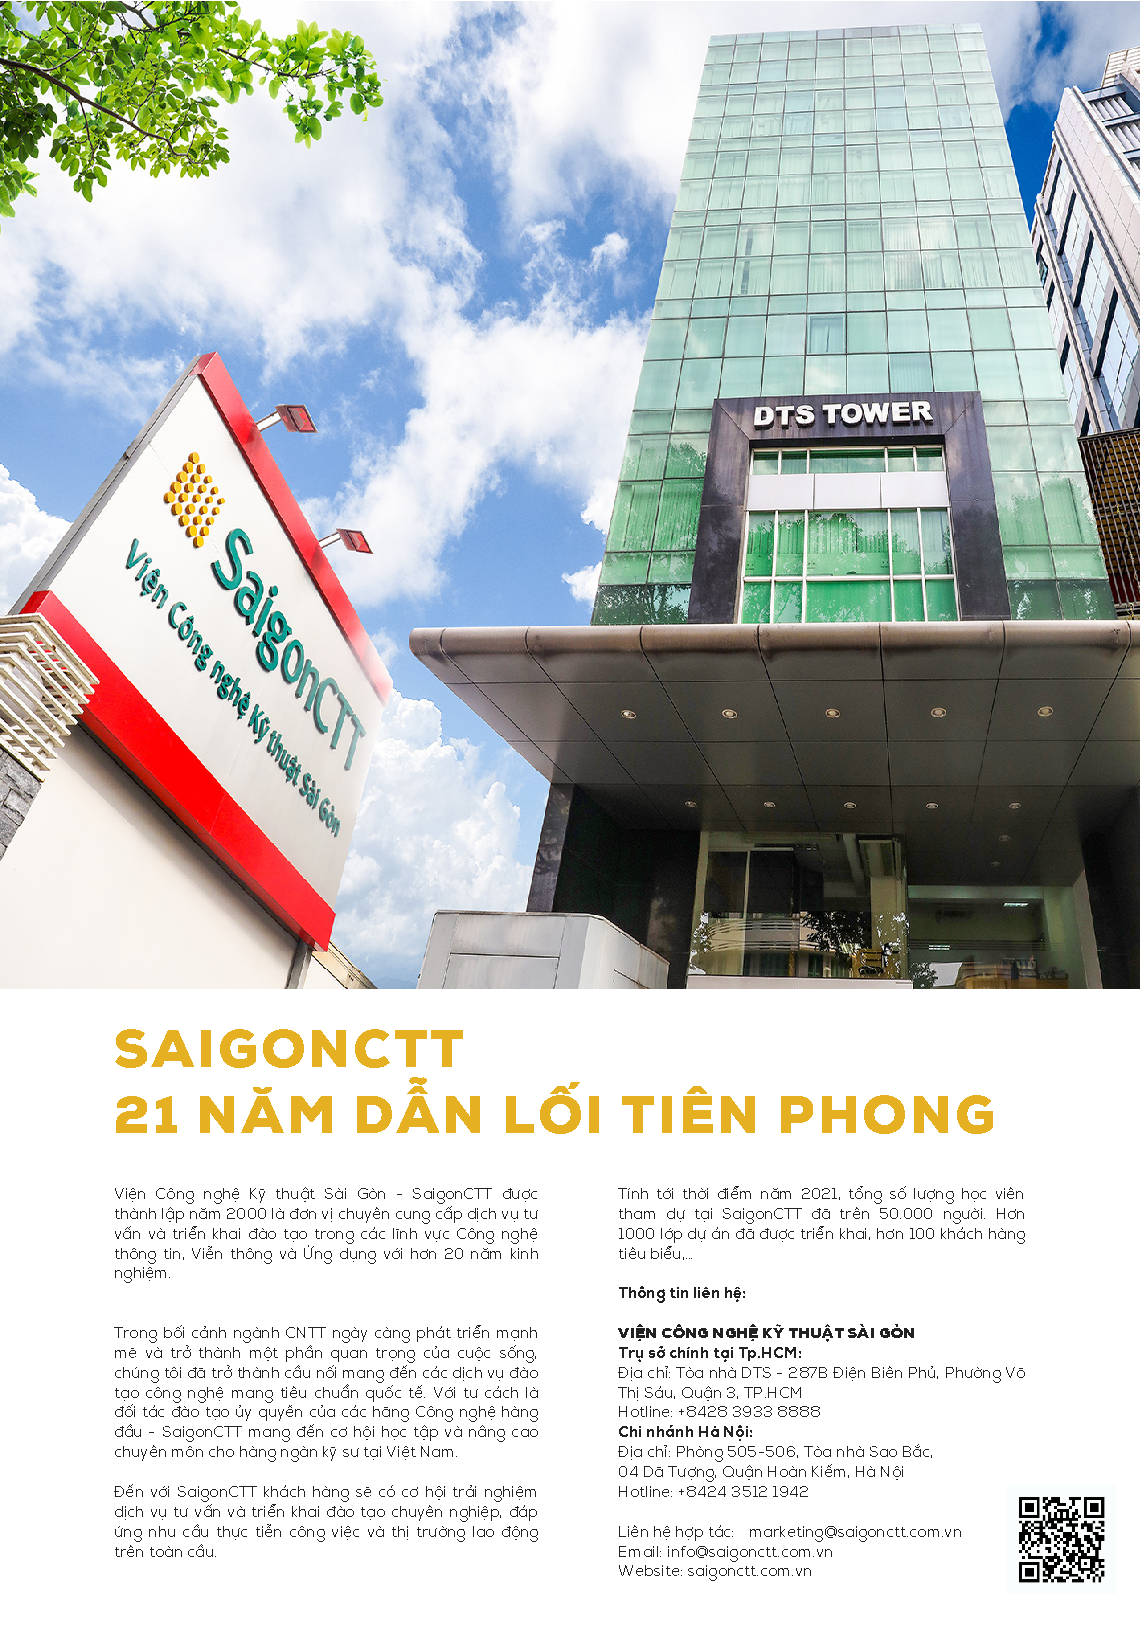
\includegraphics[scale=1]{DTS.pdf}}}
%	\centering
%	\vspace*{0cm}
%	\endgroup
%	\newpage	
%	\pagestyle{empty}
	
%	\setcounter{figure}{0}
%	\thispagestyle{toancuabinone}
\pagestyle{toancuabi}
\everymath{\color{toancuabi}}
%\blfootnote{$^1$\color{toancuabi}Đại học Thăng Long.}
\graphicspath{{../toancuabi/pic/}}
\begingroup
\AddToShipoutPicture*{\put(0,616){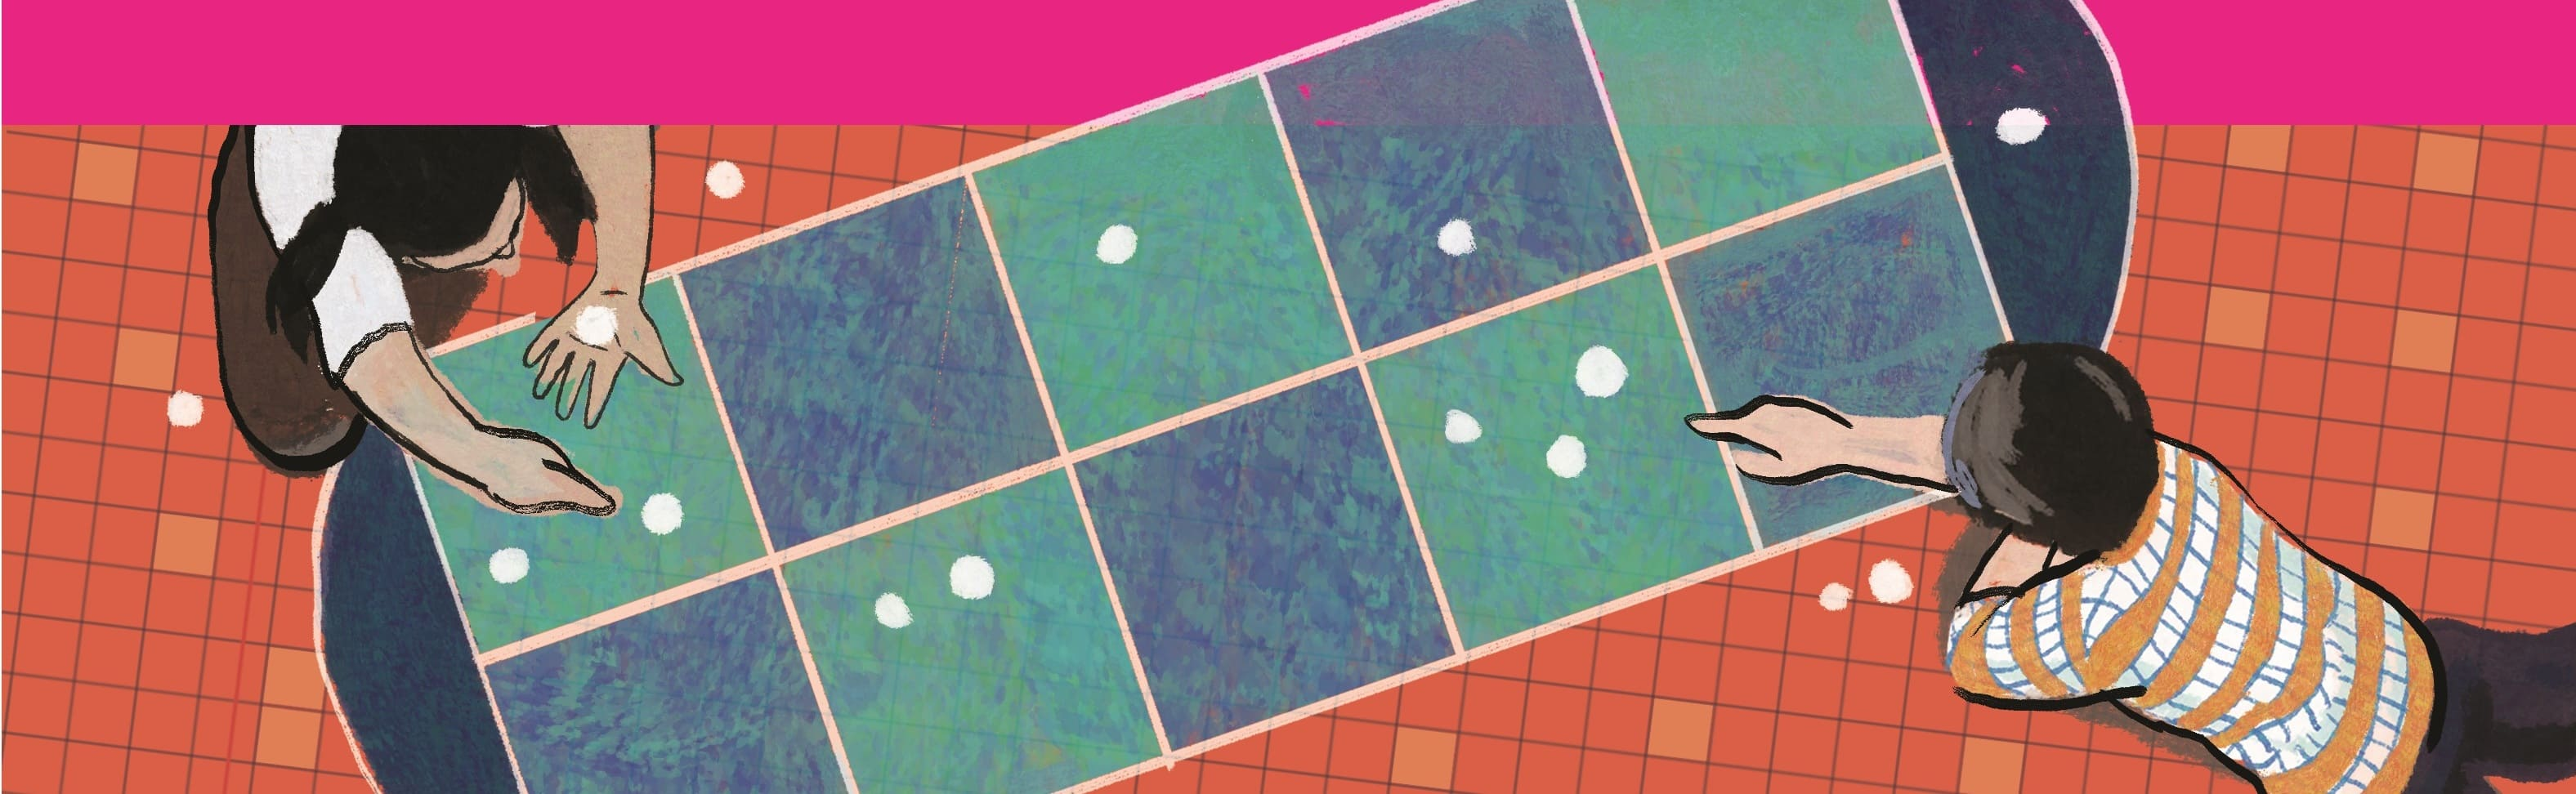
\includegraphics[width=19.3cm]{../bannertoancuabi}}}  
\AddToShipoutPicture*{\put(176,552){
\includegraphics[scale=1]{../tieude.pdf}}} 
\centering
\endgroup

\vspace*{155pt}

\begin{multicols}{2}
	Thám tử Xuân Phong trong một lần đi du lịch cùng thanh tra Lê Kính tới một hòn đảo xa xôi tận bên Phi Châu được đặt chân tới một ngôi làng đẹp tuyệt diệu ẩn sau những cành cọ, rặng dừa xum xuê chạy dài bờ biển xanh ngắt trong veo. Trưởng làng đon đả mời hai người tới ngôi nhà lớn của cả làng để dự một lễ hội đặc biệt của người dân. Theo như chỉ dẫn từ công ty lữ hành, những người thổ dân ở làng đó chia thành hai họ tộc, họ Tutu chuyên nói thật và họ Titi lại chuyên nói dối. Khi bước vào căn nhà lớn, Xuân Phong đã thấy có $50$ người dân đảo ăn mặc\hspace*{123pt}\linebreak[6]những bộ quần\hspace*{123pt}\linebreak[6]áo màu sắc lộng\hspace*{123pt}\linebreak[6]lẫy dành riêng\hspace*{123pt}\linebreak[6]cho lễ hội và\hspace*{123pt}\linebreak[6]ngồi xung quanh\hspace*{123pt}\linebreak[6]một chiếc bàn\hspace*{123pt}\linebreak[6]tròn thật to đặt\hspace*{123pt}\linebreak[6]giữa phòng. Theo\hspace*{123pt}\linebreak[6]như tục lệ, $50$\hspace*{123pt}\linebreak[6]người sẽ lần lượt\hspace*{123pt}\linebreak[6]đứng lên và nếu\hspace*{123pt}\linebreak[6]số tuổi của hai\hspace*{123pt}\linebreak[6]người ngồi cạnh\hspace*{123pt}\linebreak[6]anh ta, tuổi\hspace*{123pt}\linebreak[6]người ngồi bên\hspace*{123pt}\linebreak[6]trái trước -- sau\hspace*{123pt}\linebreak[6]đó là người ngồi\hspace*{123pt}\linebreak[6]bên phải. Xuân\hspace*{123pt}\linebreak[6]Phong được biết trước trong sách hướng dẫn du lịch là: người tộc Tutu sẽ nói đúng cả hai con số này, còn người tộc Titi sẽ tăng một trong hai số tuổi của hai người ngồi cạnh (người nào theo cách anh ta tùy thích chọn) thêm $1$ tuổi còn giảm tuổi kia đi $1$ tuổi. Xuân Phong chỉ cần nghe xong và ghi chép lại $50$ câu nói  của $50$ người dân làng ngồi quanh bàn, sau một chút suy nghĩ, đã biết được ngay ai là người đến từ tộc nào, Tutu hay Titi. Làm sao mà thám tử lại tài thế nhỉ, các em có biết cách lập luận của Xuân Phong được hay không?
	
	\vspace*{280pt}
	\insertpic{159}{86}{0.54}{xp}
\end{multicols}
\newpage
\begingroup
\AddToShipoutPicture*{\put(112,672){
\includegraphics[scale=1]{../tieude11.pdf}}} 
\centering
\endgroup
\vspace*{35pt}

\begin{multicols}{2}
	$\pmb{1.}$ Bạn Tùng làm một số bài trắc nghiệm và sau đó sẽ lấy điểm trung bình của các bài đó để tự đánh giá học lực của mình. Trả lời xong bài trắc nghiệm cuối cùng, Tùng thấy rằng nếu bài này mình được $97$ điểm bài này thì điểm trung bình của tất cả các bài trắc nghiệm sẽ là $90$ điểm, còn nếu như ở bài cuối Tùng chỉ nhận được $73$ điểm thì điểm trung bình của bạn ấy sẽ chỉ còn $87$ điểm. Vậy số bài trắc nghiệm trong loạt bài mà Tùng đã làm là bao nhiêu?
	\begin{figure}[H]
		\centering
		\vspace*{-10pt}
		\captionsetup{labelformat= empty, justification=centering}
		
\includegraphics[width=0.95\linewidth]{Pi12_Bai1}
		\vspace*{-10pt}
	\end{figure}
	\vskip 0.1cm
	$\pmb{2.}$ Có $3$ loại kẹo để trong lọ thủy tinh với ba màu khác nhau: kẹo màu đỏ, kẹo màu vàng và kẹo màu trắng. Nếu Bình nhặt hết số kẹo màu vàng thì tổng số kẹo trong lọ ít hơn một chiếc so với $2/3$ tổng số kẹo ban đầu. Còn nếu Bình nhặt hết số kẹo đỏ, thì số kẹo còn lại trong lọ nhiều hơn $4$ chiếc so với $2/3$ tổng số kẹo ban đầu.
	\vskip 0.1cm
	Vậy ban đầu trong hai loại kẹo màu vàng và kẹo màu trắng, loại nào có nhiều và nhiều hơn bao nhiêu?
	\begin{figure}[H]
		\centering
		\vspace*{-10pt}
		\captionsetup{labelformat= empty, justification=centering}
		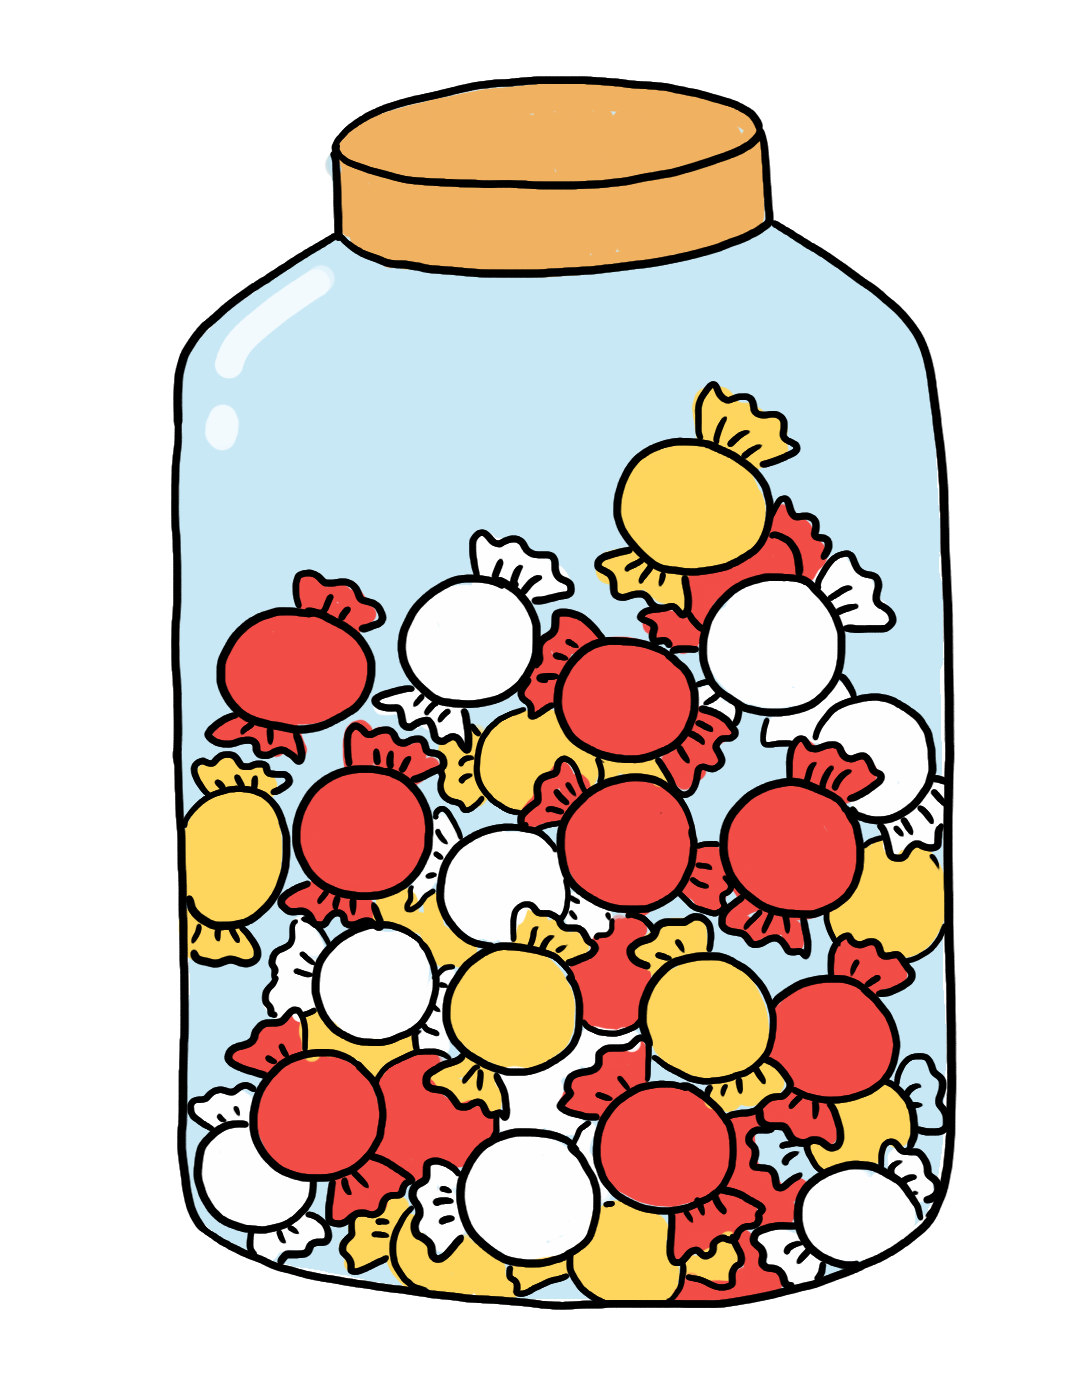
\includegraphics[width=0.45\linewidth]{Pi12_Bai2}
		\vspace*{-15pt}
	\end{figure}
	$\pmb{3.}$ $40$ bạn nhỏ nắm tay nhau xếp thành vòng tròn quanh đống lửa trại. Có tất cả $22$ bạn có nắm tay một bạn nam, và $30$ bạn có nắm tay một bạn nữ. Hỏi có tất cả bao nhiêu bạn nữ xếp trong vòng tròn quanh lửa trại ngày hôm đó?
	\begin{figure}[H]
		\centering
		\vspace*{-10pt}
		\captionsetup{labelformat= empty, justification=centering}
		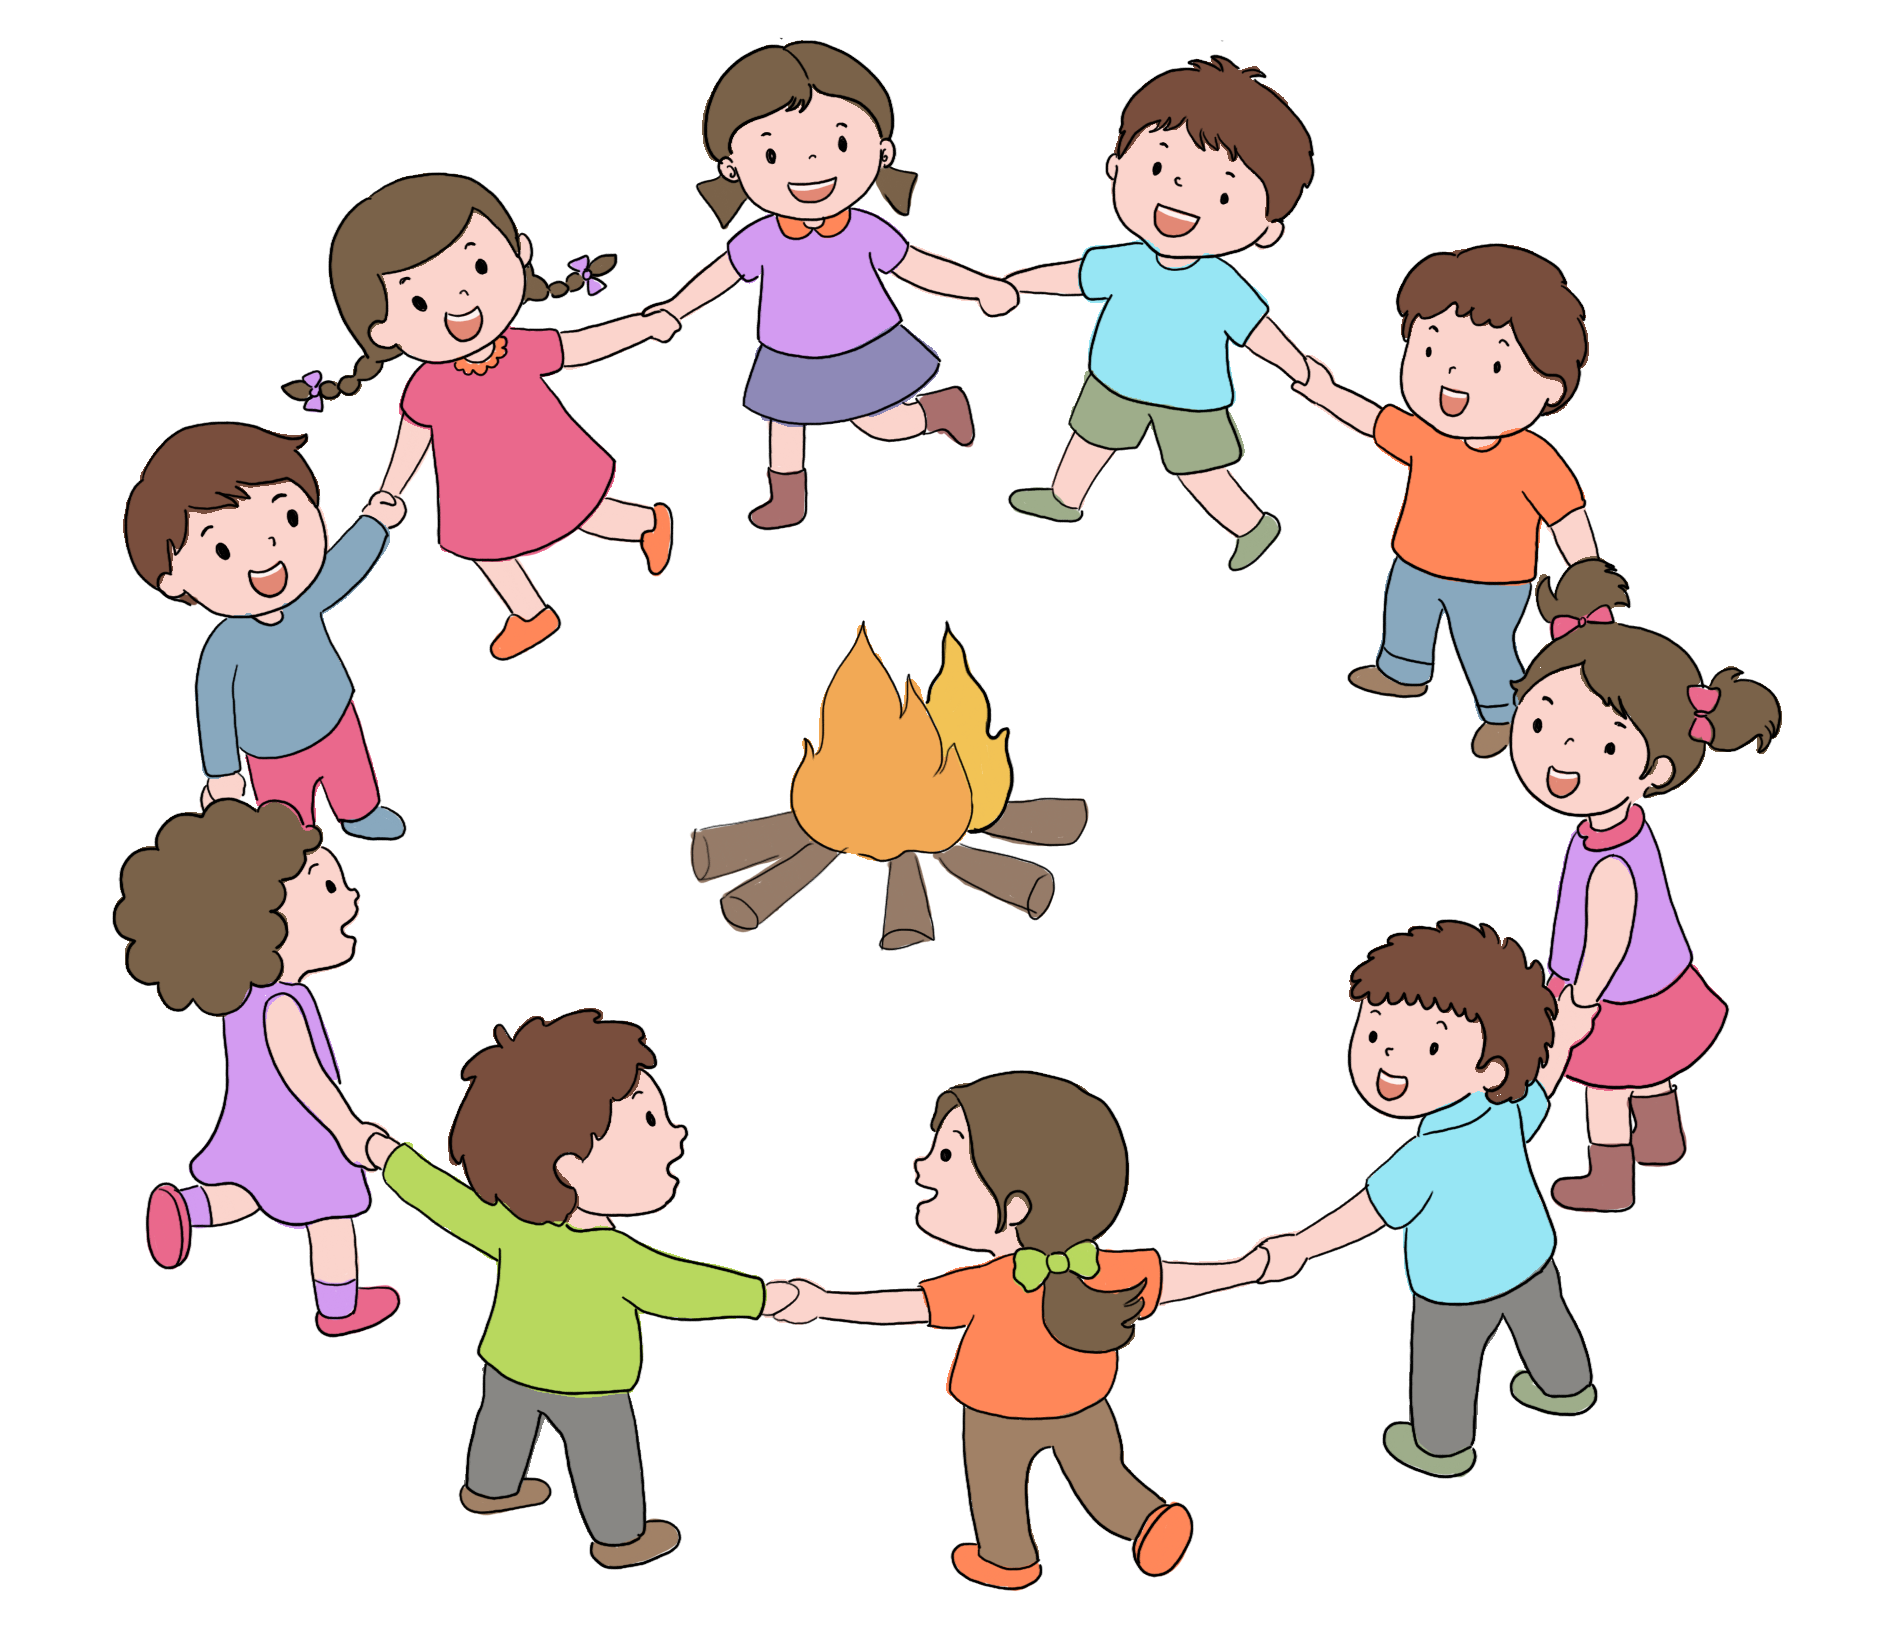
\includegraphics[width=0.9\linewidth]{Pi12_Bai3}
		\vspace*{-10pt}
	\end{figure}
	$\pmb{4.}$ Trên mặt bàn có $5$ đồng xu xếp thành hàng ngang. Đồng xu ở giữa đặt xấp còn $4$ đồng còn lại đều đặt ngửa. Mỗi một lần em được cho phép lật $3$ đồng xu đặt liền nhau tùy ý. Liệu em có thể có cách lật thế nào để cuối cùng $5$ đồng xu đều đặt xấp được không?
	\vskip 0.1cm
	Cũng câu hỏi như vậy, nếu lúc đầu đồng xu đặt xấp duy nhất là đồng xu xếp đầu hàng? Là đồng xu xếp thứ hai trong hàng?
	\begin{figure}[H]
		\centering
		\vspace*{-5pt}
		\captionsetup{labelformat= empty, justification=centering}
		
\includegraphics[width=1\linewidth]{Pi12_Bai4}
		\vspace*{-20pt}
	\end{figure}
	$\pmb{5.}$ Một lần Lý Toét diện guốc mộc loẹt quẹt ra tận chợ phiên chơi ngày cuối tuần. Khi về nhà, Lý Toét ba hoa khoe khắp làng ``Tôi là tôi gặp $15$ ông bán cây cảnh ngoài chợ nhé. Mà tôi đi lòng vòng và nghiệm thấy cứ $3$ ông bất kỳ có tổng cộng đúng $10$ cây hoa hồng. Thế là tôi lẩm nhẩm đoán được ngay $15$ ông này có tất cả bao nhiêu cây hoa hồng."
	\vskip 0.1cm
	Em có thể đoán được như Lý Toét xem $15$ ông bán cây có tất cả bao nhiêu cây hoa hồng không? Hay Lý Toét có khoác lác hay nhầm lẫn gì không nhỉ?
	\begin{figure}[H]
		\centering
%		\vspace*{1pt}
		\captionsetup{labelformat= empty, justification=centering}
		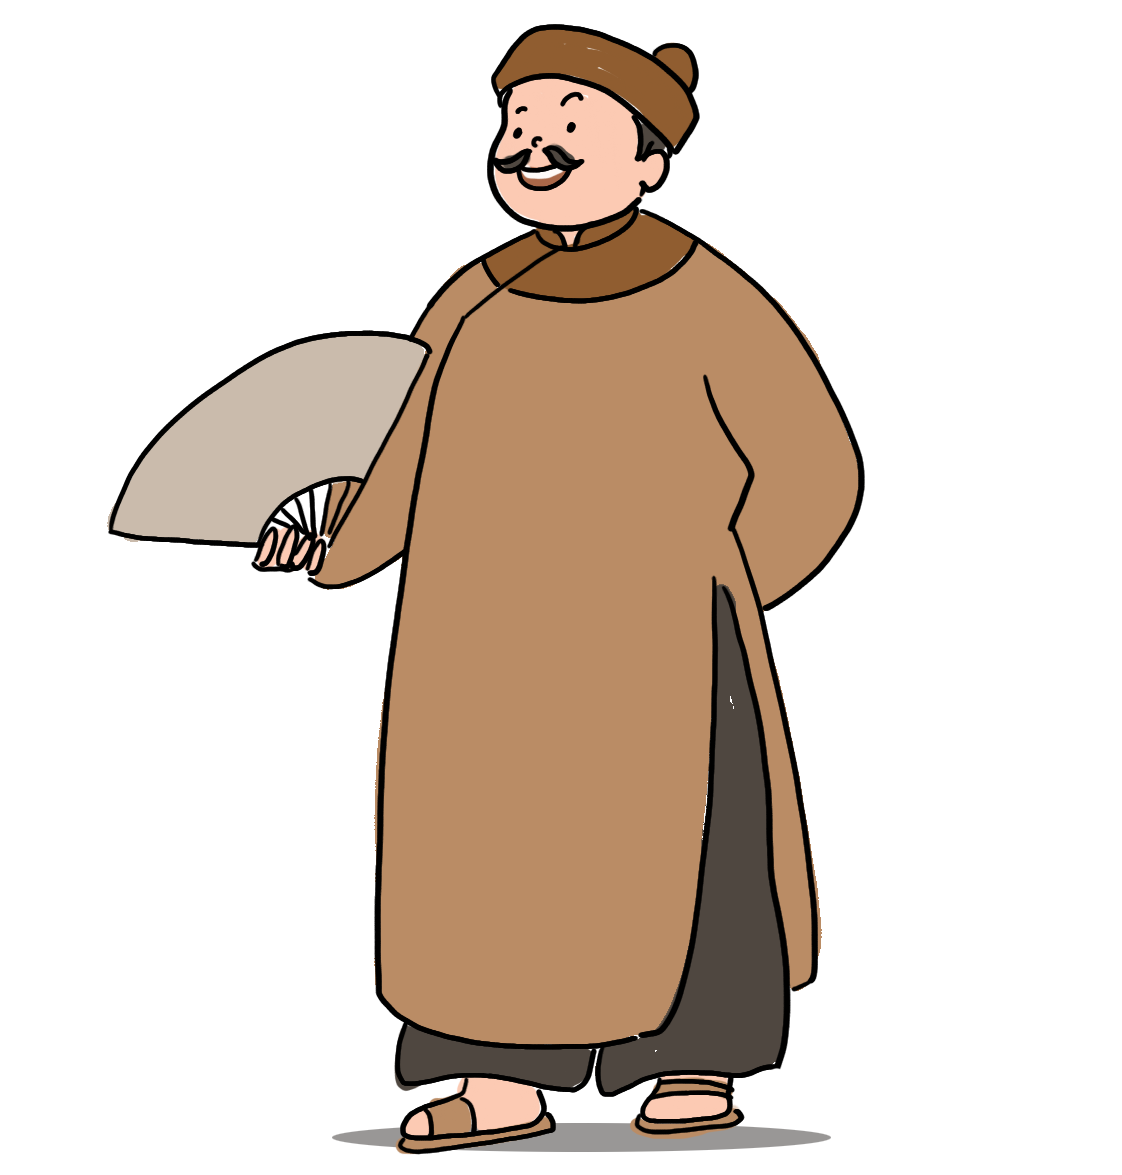
\includegraphics[width=0.58\linewidth]{Pi12_Bai5}
		\vspace*{-15pt}
	\end{figure}
	$\pmb{6.}$ Có $20$ bạn tham gia nhóm Toán ngồi xung quanh một chiếc bàn tròn. Một lúc sau các bạn nhóm Văn cũng đến, cứ xen kẽ hai bạn nhóm Toán ngồi kề nhau giờ có thêm $20$ bạn mới từ nhóm Văn. Tổng cộng có tất cả $400$ bạn từ nhóm Văn ngồi thêm quanh chiếc bàn tròn rộng đó. Thỉnh thoảng một bạn nhóm Văn lại đứng dậy và rời khỏi bàn, dắt theo hai bạn ngồi cạnh mình đi luôn. Cứ như vậy, sau một lúc thì quanh bàn số bạn nhóm Toán còn lại chỉ là $3$ bạn. Hỏi số bạn nhóm Văn còn ở lại quanh bàn lúc đó ít nhất phải là bao nhiêu?
\end{multicols}
\vspace*{-12pt}
\rule{1\linewidth}{0.1pt}
\begingroup
\AddToShipoutPicture*{\put(112,452){
\includegraphics[scale=1]{../tieude2.pdf}}} 
\centering
\endgroup
\graphicspath{{../toancuabi/pic/}}
\vspace*{80pt}

\begin{multicols}{2}
	$\pmb{1.}$ Có $30$ bạn học sinh tham gia một cuộc thi hùng biện bằng tiếng Anh. Các bạn lần lượt chọn các câu hỏi và trả lời theo thứ tự xếp hàng. Bạn thứ nhất được $80$ điểm, bạn thứ hai được $60$ điểm, bạn thứ ba có số điểm bằng trung bình cộng của bạn thứ nhất và bạn thứ hai, bạn thứ tư có số điểm bằng trung bình cộng của ba bạn đầu tiên. Nói chung, kể từ bạn thứ ba trở đi thì  mỗi một bạn học sinh tiếp theo luôn có số điểm bằng trung bình cộng số điểm của các bạn đã thi trước đó. 
	\vskip 0.1cm
	Hỏi bạn cuối cùng, tức bạn có số thứ tự $30$, đạt được bao nhiêu điểm trong cuộc thi? 
	\begin{figure}[H]
		\centering
		\vspace*{-10pt}
		\captionsetup{labelformat= empty, justification=centering}
		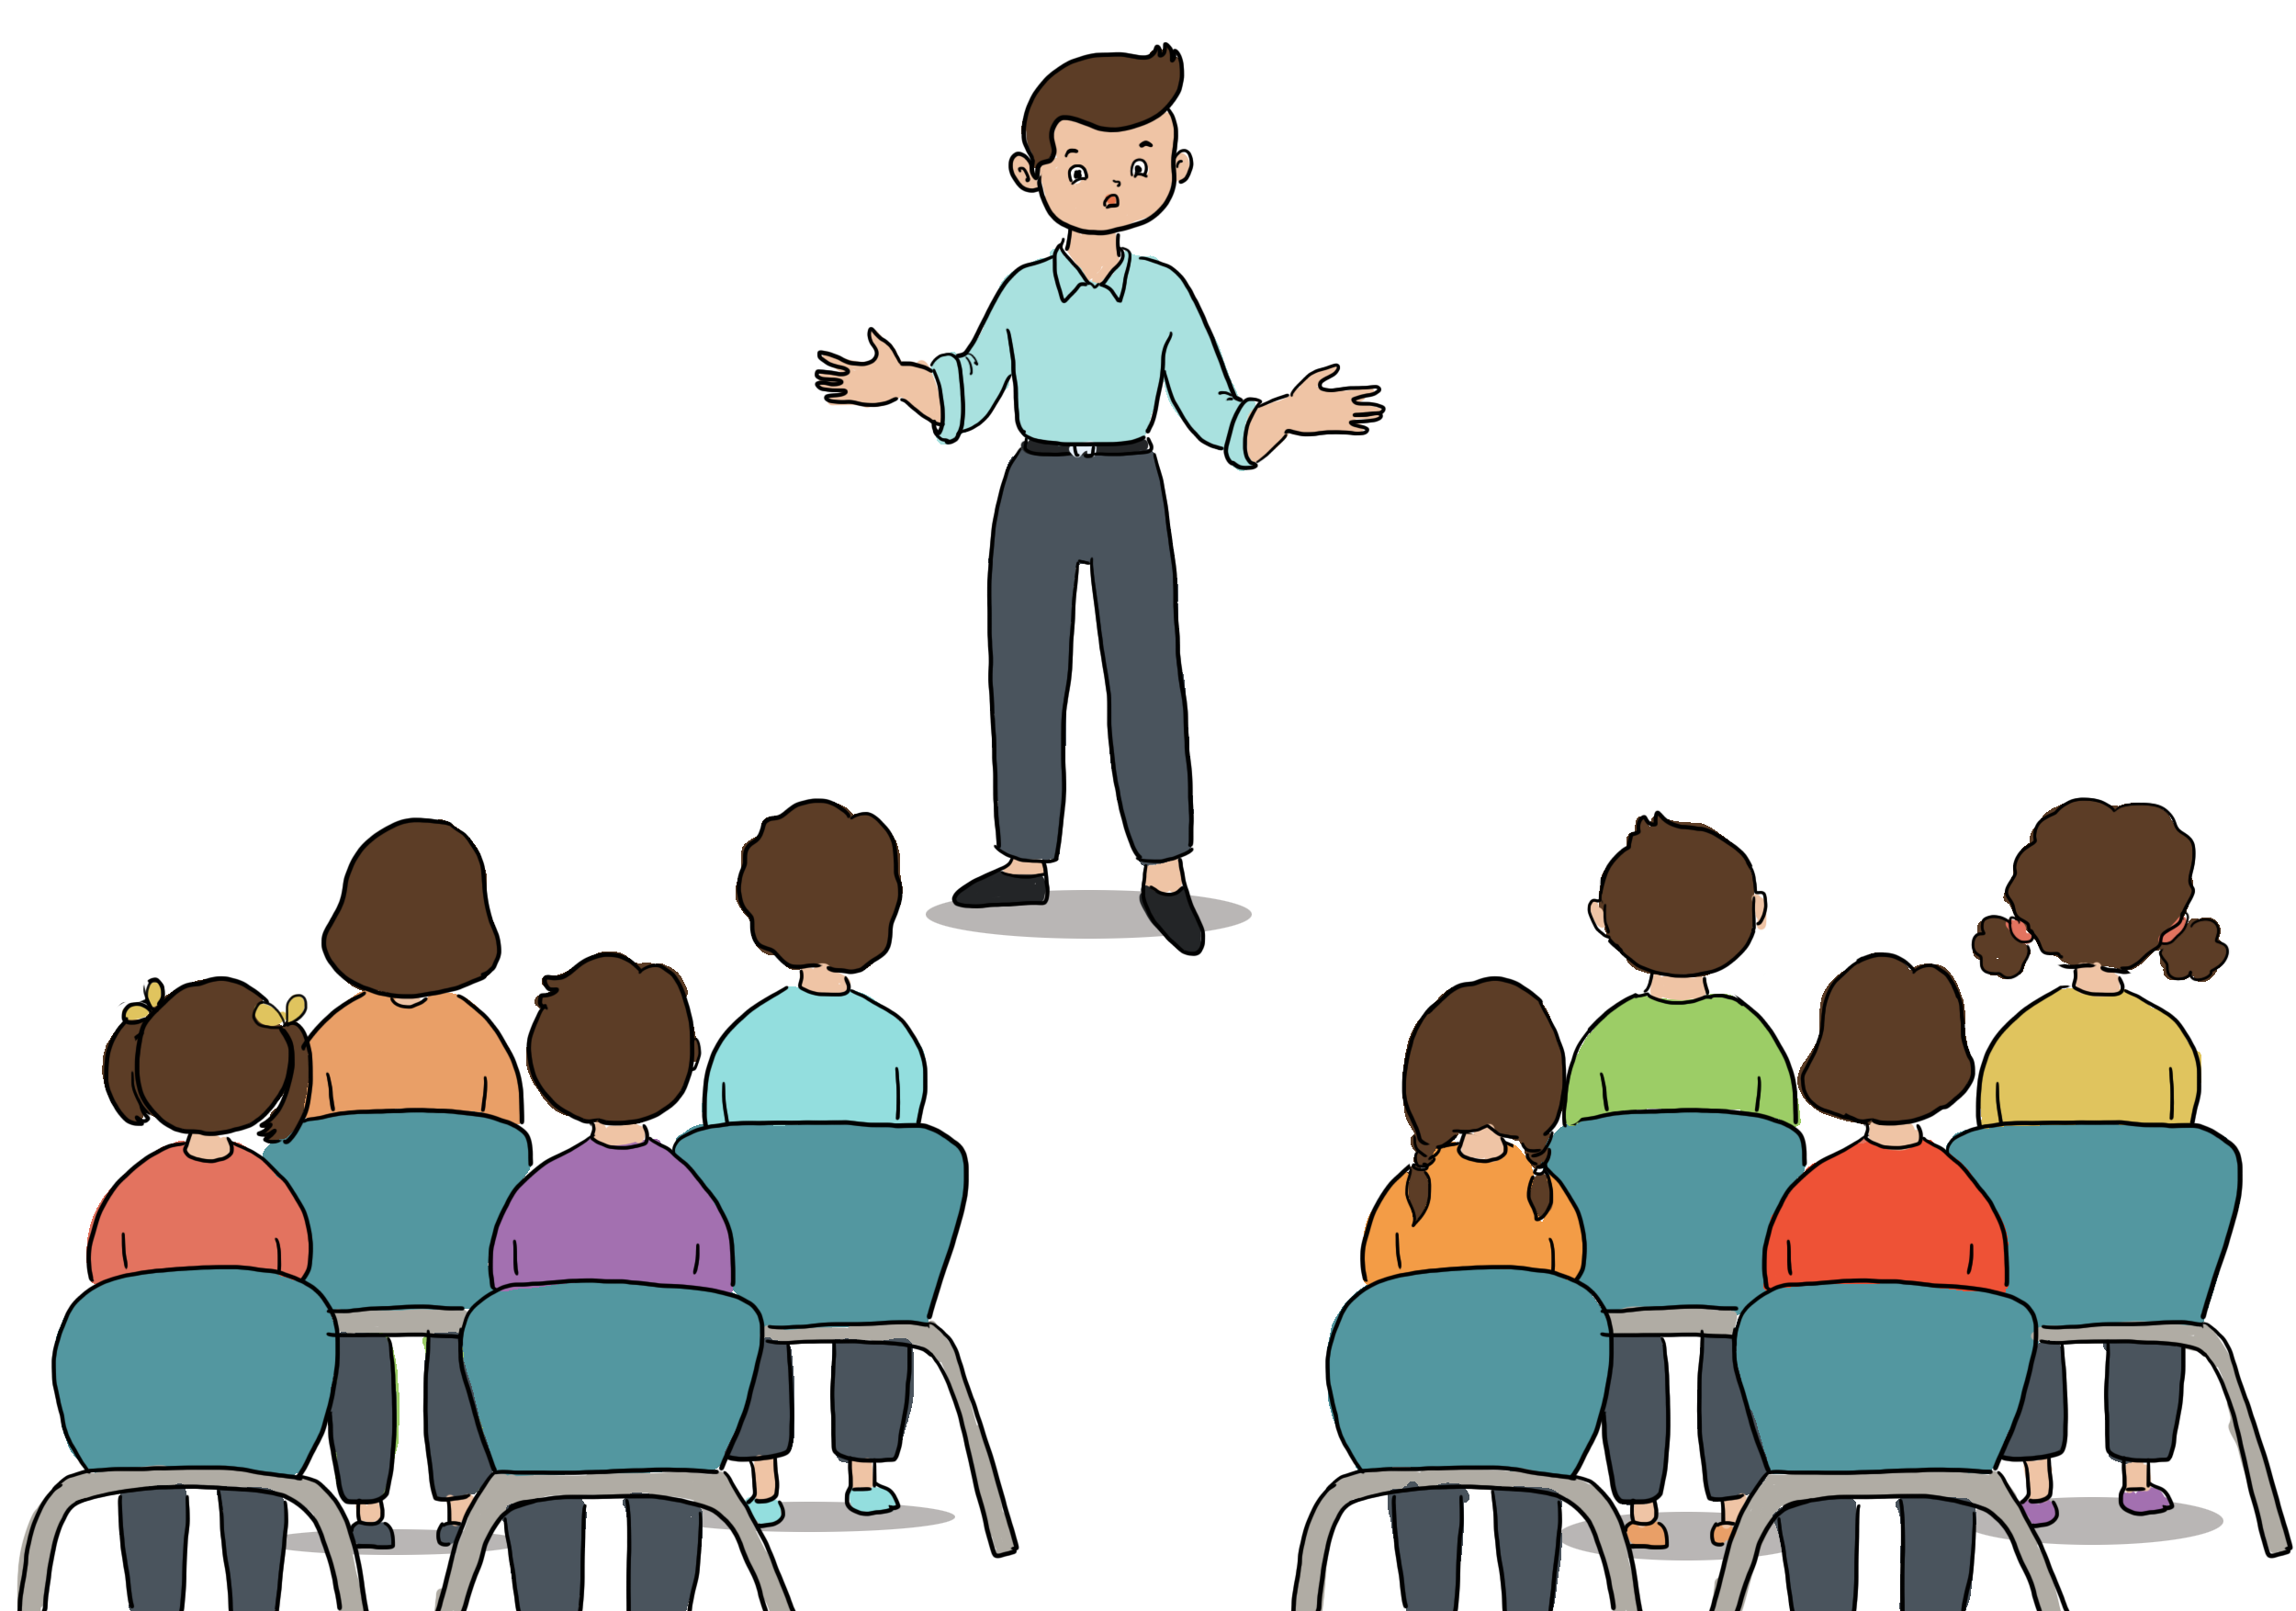
\includegraphics[width=0.92\linewidth]{bai1}
		\vspace*{-10pt}
	\end{figure}
	\textit{Lời giải.} 	Ta nhận thấy nếu mỗi bạn tiếp theo nhận được số điểm là trung bình cộng điểm số của các bạn đứng trước đó, thì trung bình cộng số điểm của các bạn luôn không thay đổi. Nếu hai bạn đầu tiên có trung bình cộng số điểm là $70$, thì kể từ bạn thứ ba, trung bình cộng số điểm của $n$ bạn đầu tiên, ($2\!<\!n\!<\!30$), luôn bằng $70$. Vì thế bạn cuối cùng cũng nhận được $70$ điểm.
	\vskip 0.1cm
	$\pmb{2.}$ Vào một ngày hè, ba bạn Yến, Vinh và Công đến hiệu kem và mỗi bạn đều lấy đủ $3$ vị: trái cây, vani và sô--cô--la (mỗi vị một cốc). Sau khi ăn xong, vì $3$ cốc cho một người là chưa đủ, nên Yến lấy thêm một cốc kem trái cây, Vinh lấy thêm một cốc kem vani và Công lấy thêm một cốc kem sô--cô--la. 
	\begin{figure}[H]
		\centering
		\vspace*{-10pt}
		\captionsetup{labelformat= empty, justification=centering}
		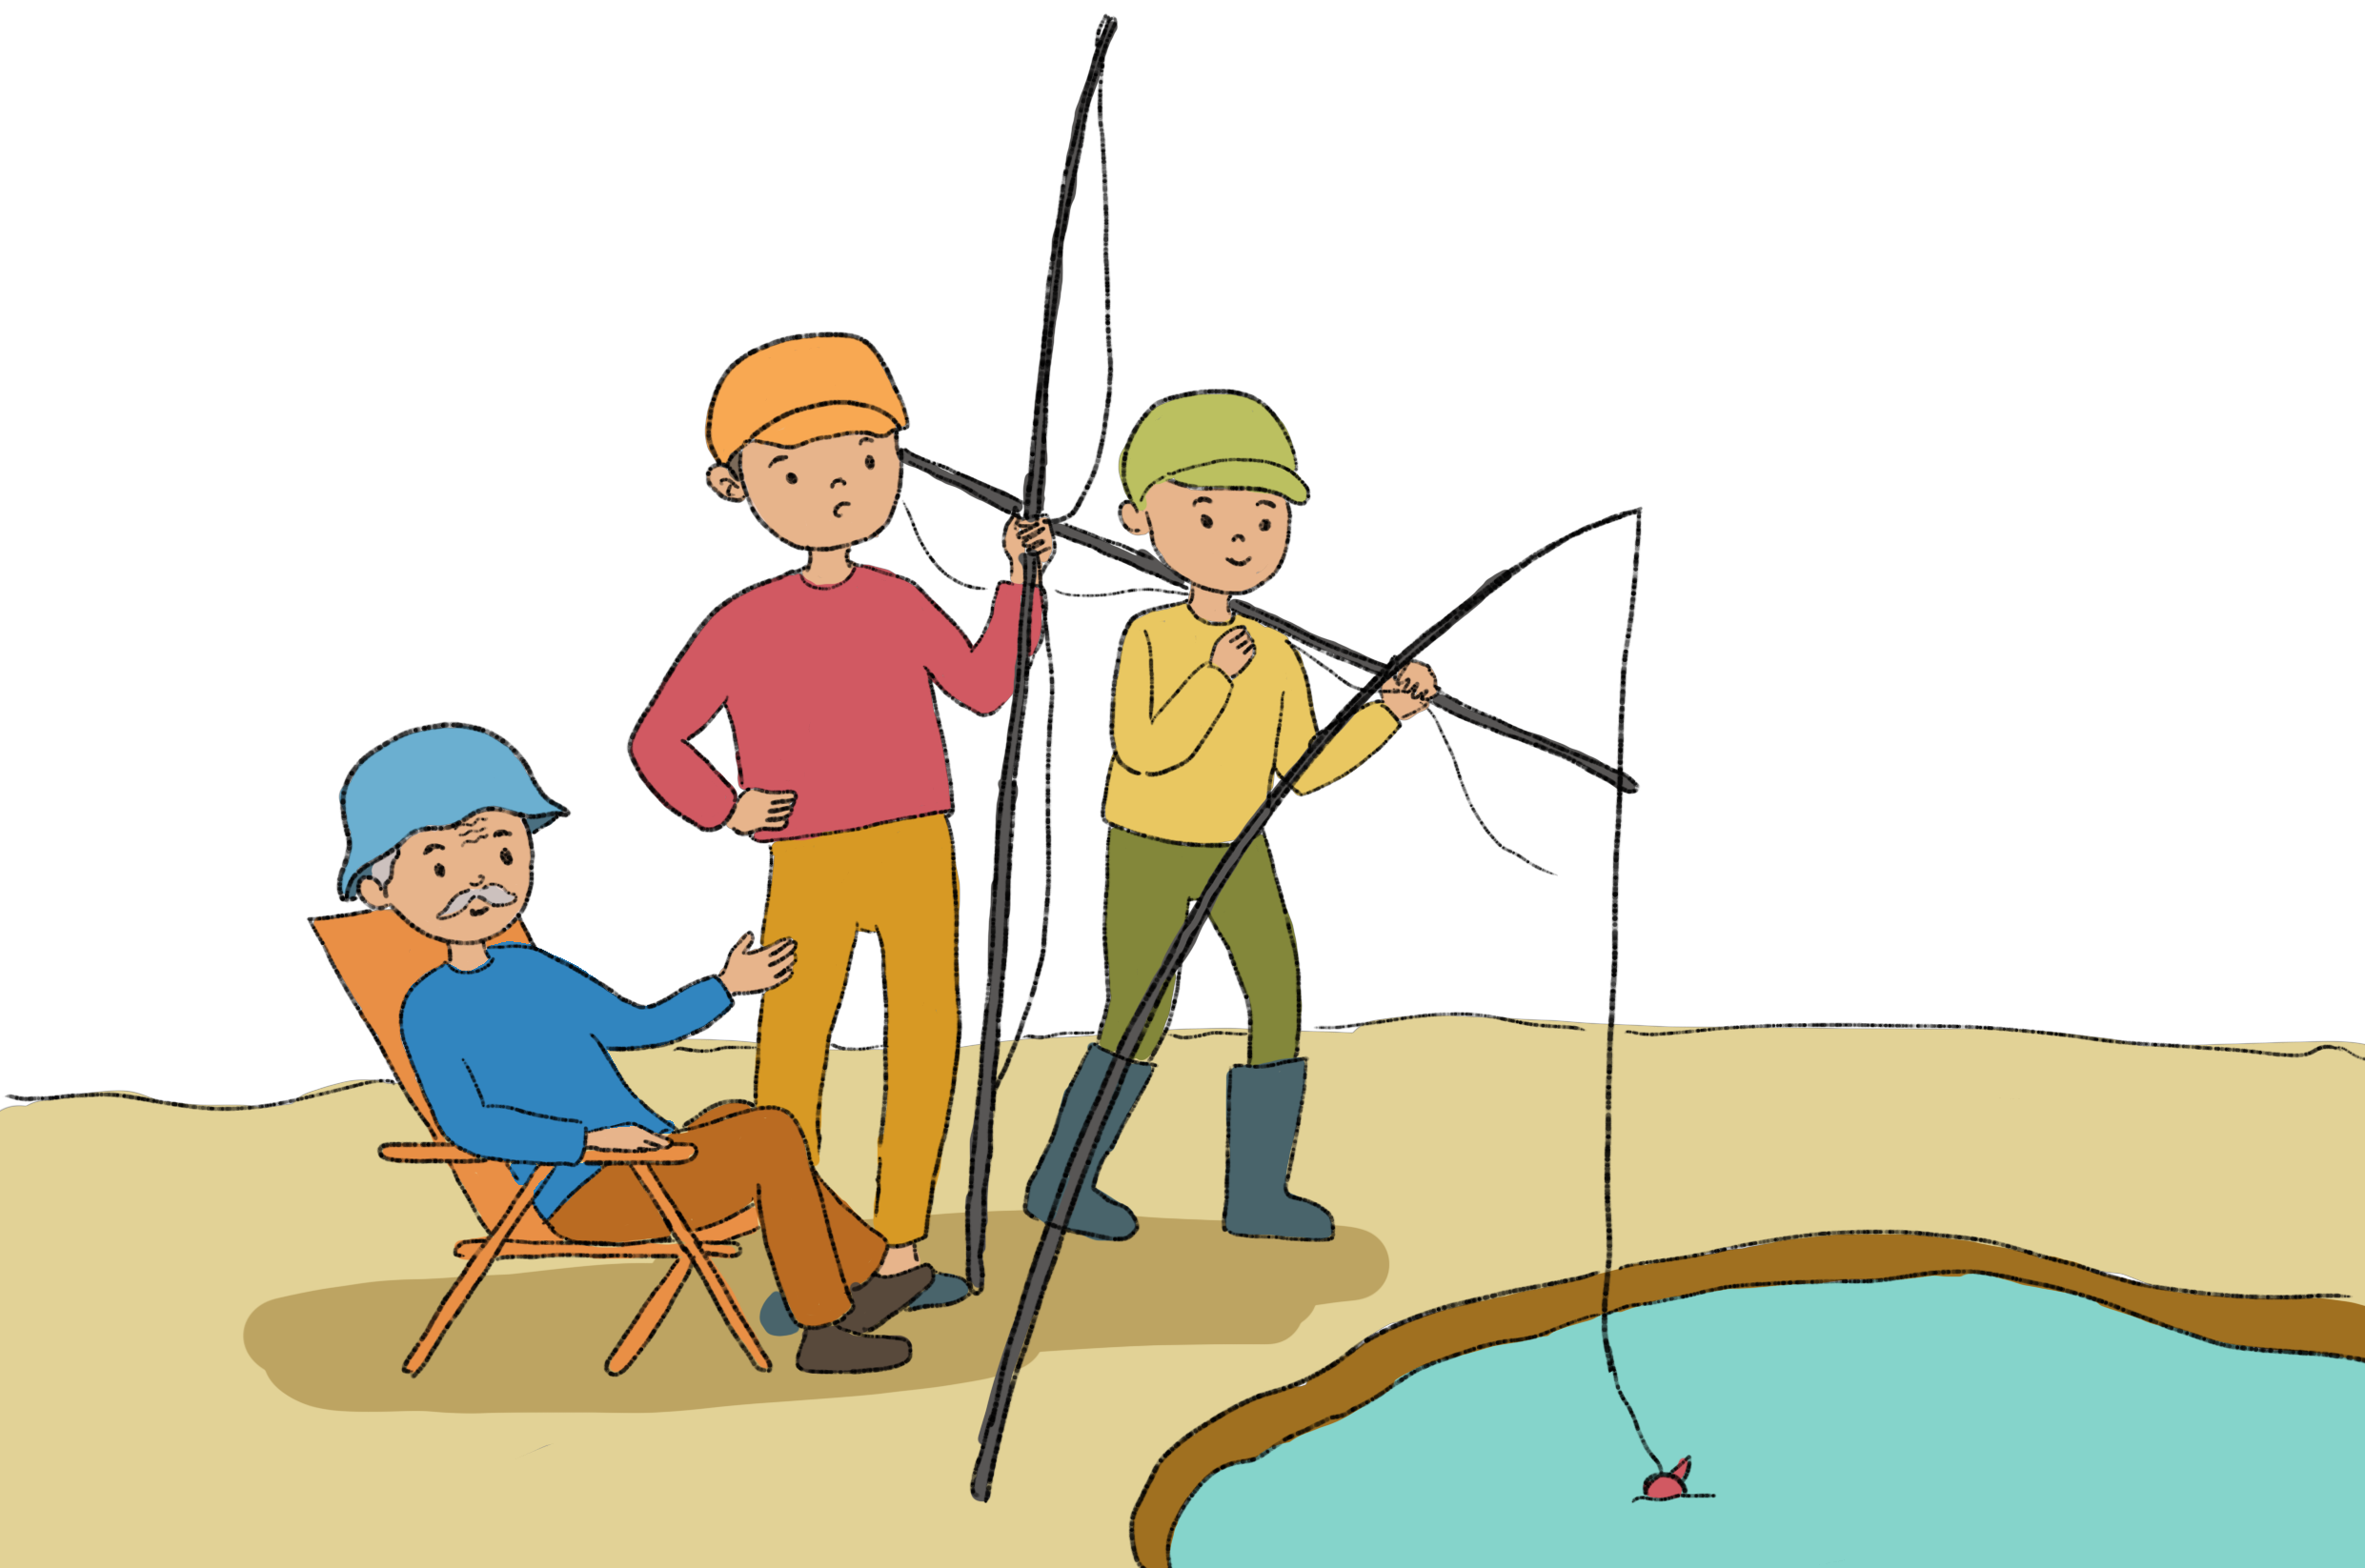
\includegraphics[width=0.92\linewidth]{bai2}
		\vspace*{-10pt}
	\end{figure}
	Lúc ra quầy thanh toán, Yến phải trả $70$ nghìn, Vinh phải trả $80$ nghìn còn Công phải trả $90$ nghìn. Hỏi mỗi vị kem có giá bao nhiêu tiền một cốc?
	\vskip 0.1cm
	\textit{Lời giải.} 	Gọi $a$ là giá tiền một cốc kem hoa quả, khi đó $a+10000$ là giá một cốc kem va--ni, còn $a+20000$ là giá một cốc kem sô--cô--la. Tổng số tiền các bạn phải trả là $70+80+90= 240$ (nghìn đồng). Tổng số này cũng bằng $4(a+a+10000+a+20000)= 12 a+ 120000$.
	\vskip 0.1cm 
	Từ đây suy ra $a= 10000$.
	\vskip 0.1cm 
	Như vậy một cốc kem hoa quả giá $10$ nghìn đồng, một cốc kem va--ni giá $20$ nghìn đồng, còn một cốc kem sô--cô--la giá $30$ nghìn đồng. 
	\vskip 0.1cm
	\textit{Cách giải khác (Cô Hồng)}: Tổng số cốc kem mỗi loại mà ba bạn Yến, Vinh, Công đã ăn là $4$ cốc, và tổng số tiền ba bạn đã trả là 
	\begin{align*}
		70 + 80 +90 = 240 \text{ (nghìn đồng).}
	\end{align*}
	Như vậy, tổng giá tiền của $1$ cốc kem hoa quả, $1$ cốc kem va--ni và $1$ cốc kem sô--cô--la là:
	\begin{align*}
		240 : 4=60 \text{ (nghìn đồng).}
	\end{align*}
	Do đó giá tiền của $1$ cốc kem hoa quả là:
	\begin{align*}
		70-60 = 10 \text{ (nghìn đồng).}
	\end{align*}
	Giá tiền của $1$ cốc kem va--ni là:
	\begin{align*}
		80-60 = 20 \text{ (nghìn đồng).}
	\end{align*}
	Và giá tiền $1$ cốc kem sô--cô--la là:
	\begin{align*}
		90-60 = 30 \text{ (nghìn đồng).}
	\end{align*}
	$\pmb{3.}$ Ba chú khỉ con dễ thương có tên là Bibi, Bobo, và Bubu được diện áo và giày thật đẹp để quay video đăng YouTube. Các chú được mặc ba chiếc áo có các màu khác nhau là đỏ, xanh lá cây và xanh lơ. Giày của ba chú cũng có ba màu như thế, mỗi chú mang một màu. Bibi thì diện áo và giày có cùng màu. Bobo lại không thích màu đỏ, nên cả giày và áo đều không phải đỏ. Bubu thì mang giày xanh lá cây, còn áo lại khác màu giày. Vậy các chú khỉ đã mặc áo và đi giày có màu như thế nào nhỉ?
	\begin{figure}[H]
		\centering
		\vspace*{-5pt}
		\captionsetup{labelformat= empty, justification=centering}
		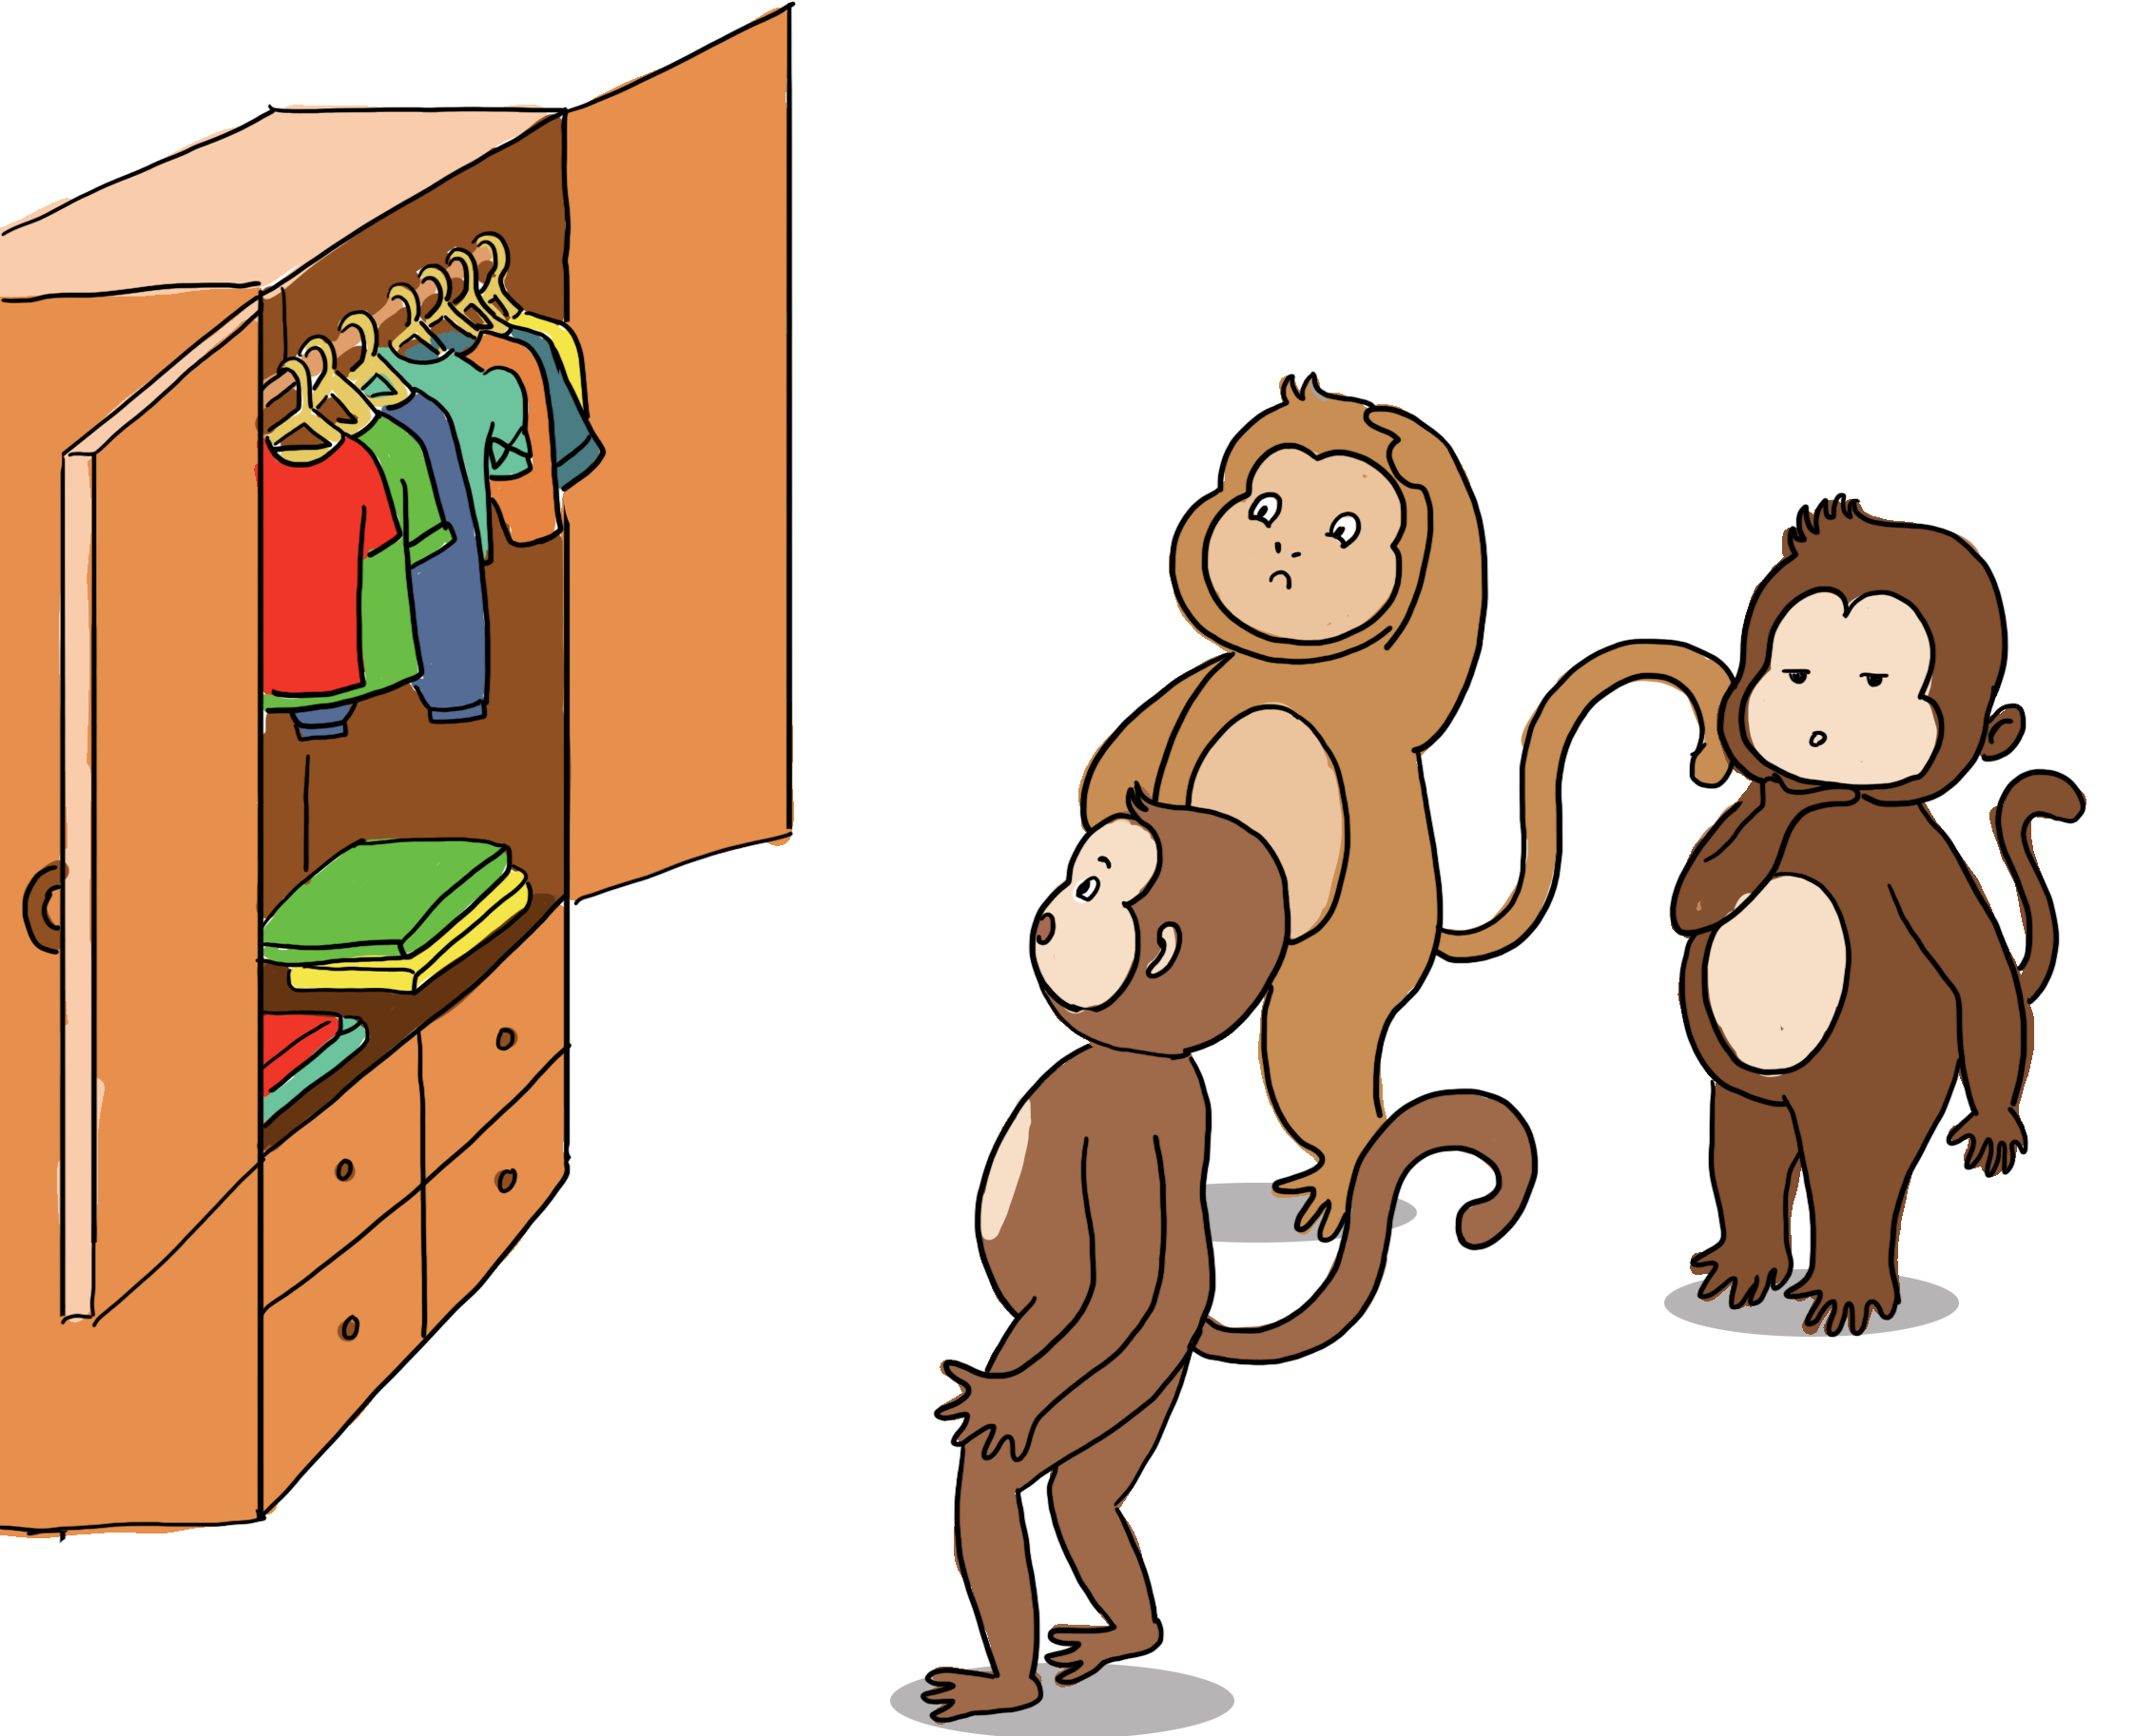
\includegraphics[width=1\linewidth]{bai3}
		\vspace*{-18pt}
	\end{figure}
	\textit{Lời giải.} Các em thấy ngay chỉ có Bibi mới mang giày màu đỏ, vì ngoài chú ta ra không có chú khỉ nào còn lại có thể mang giày đỏ. Vì thế Bibi mặc cả bộ áo và giày đều đỏ. Và suy ra Bubu phải mặc áo màu xanh lơ. Cuối cùng, ta thấy Bobo mặc áo xanh lá cây và đi giày màu xanh lơ. Các chú trông thật vui mắt khi lên hình, phải không nào các em?
	\vskip 0.1cm
	$\pmb{4.}$ Để chuẩn bị cho cuộc đua xe đạp sắp diễn ra, sáng sớm Gấu con đã mang xe ra tập luyện. Lúc đi tốc độ của Gấu con là $15$ dặm/giờ. Do đường khá đông nên chiều trở về dù vẫn đi trên con đường đó nhưng Gấu con chỉ di chuyển với tốc độ $10$ dặm/giờ. Hỏi trên cả quãng đường lúc đi và về vận tốc trung bình của Gấu con là bao nhiêu?
	\begin{figure}[H]
		\centering
		\vspace*{-5pt}
		\captionsetup{labelformat= empty, justification=centering}
		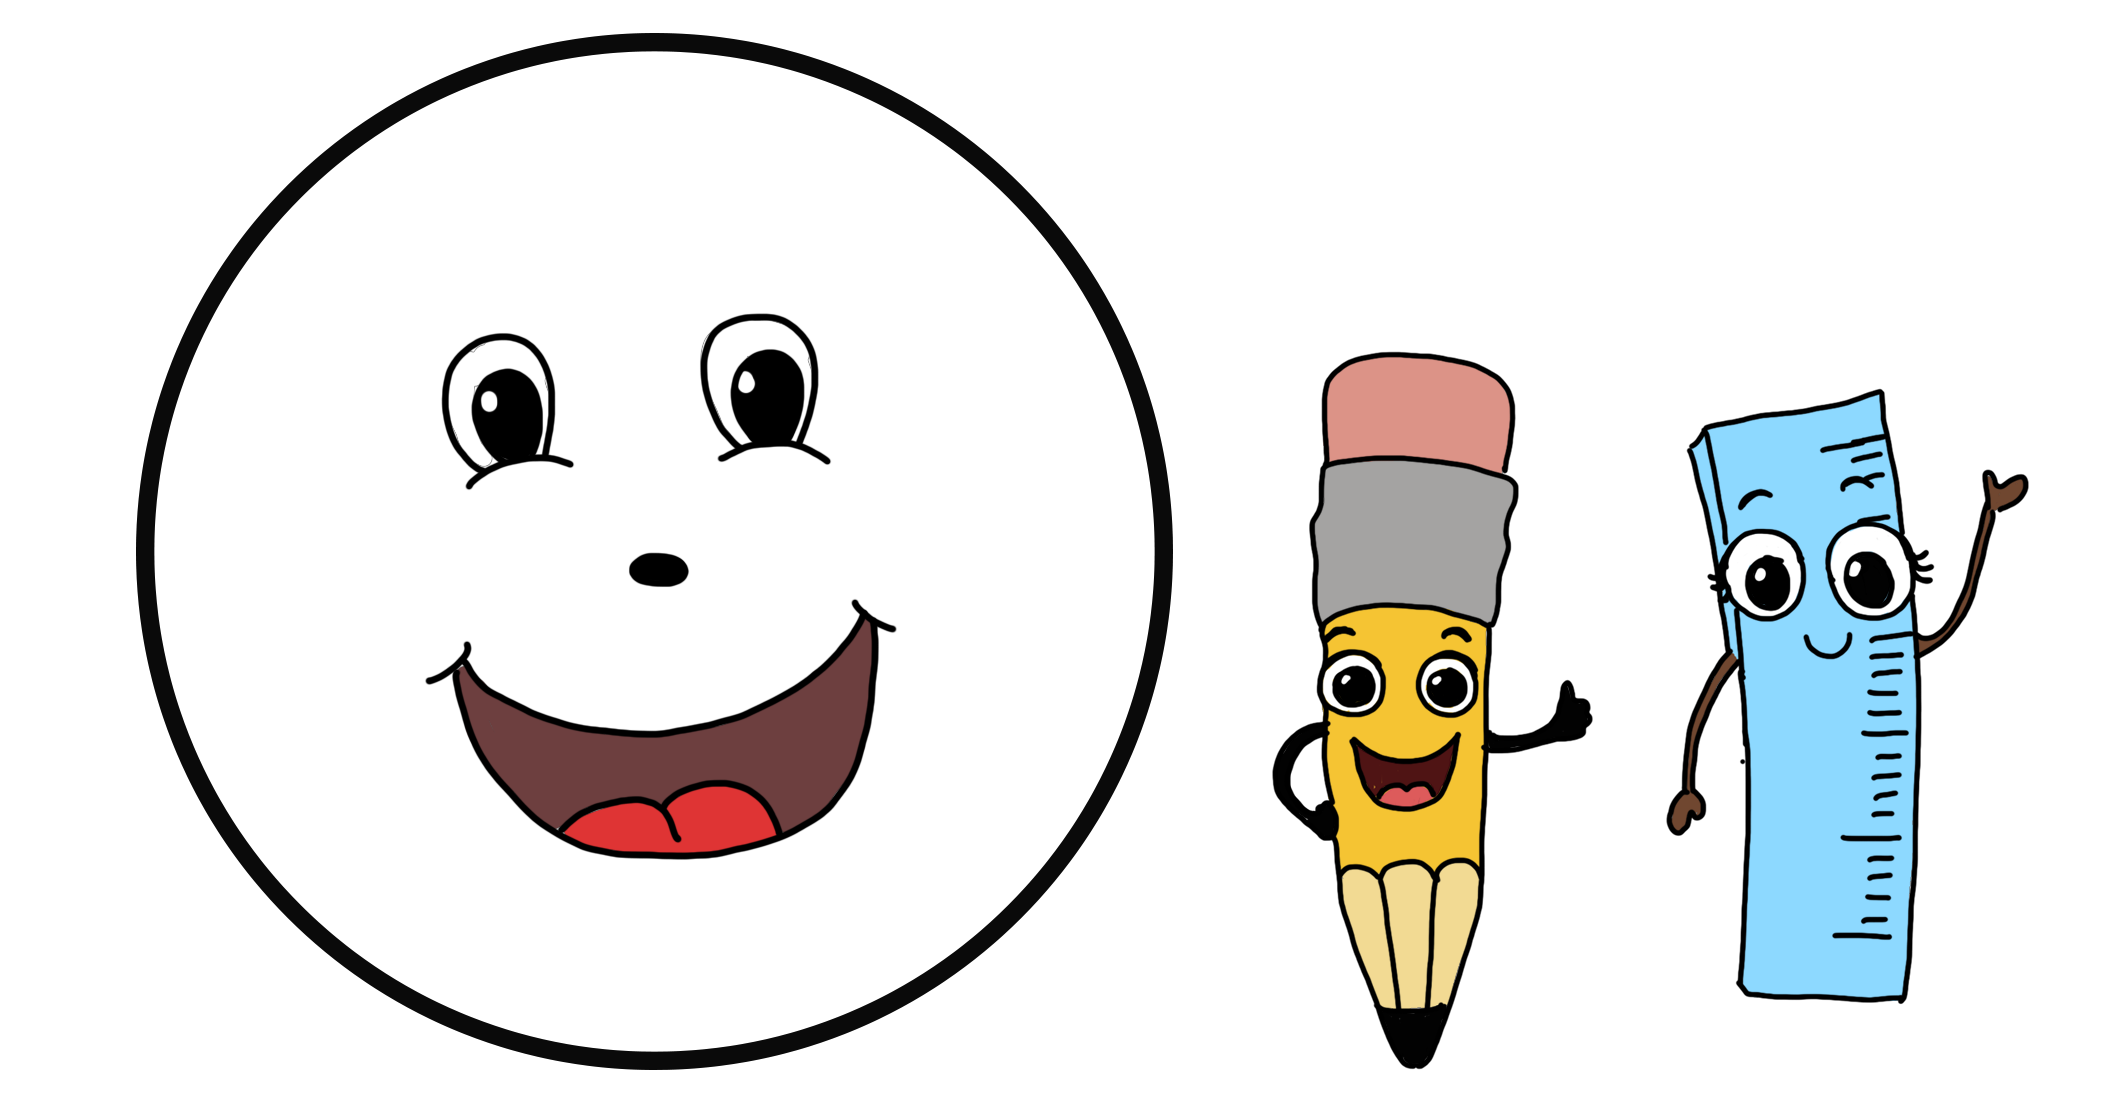
\includegraphics[width=1\linewidth]{bai4}
		\vspace*{-18pt}
	\end{figure}
	\textit{Lời giải.} 	Nhận thấy nếu quãng đường có khác nhau cũng ko ảnh hưởng tới kết quả tính vận tốc trung bình. Giả sử quãng đường là $30$ dặm, thời gian lúc đi của Gấu là:
	\begin{align*}
		30:15 =  2 \text{ (giờ).}
	\end{align*}
	Thời gian lúc về là
	\begin{align*}
		30:10 = 3 \text{ (giờ).}
	\end{align*}
	Vậy Gấu con đã đi tổng cộng $60$ dặm trong $5$ giờ nên vận tốc trung bình là
	\begin{align*}
		60:5 = 12 \text{ (dặm/giờ).}
	\end{align*}
	$\pmb{5.}$ Trên bàn có một đống đá cuội gồm $1001$ viên. Người ta lấy ra một viên đá và chia đống đá ra  thành hai đống mới, sao cho mỗi đống có ít nhất $3$ viên. Bây giờ, trong mỗi một đống đá mới, người ta lại lấy ra một viên đá và chia đống đó ra thành hai đống mới, và cứ tiếp tục như vậy. Hỏi có thể lấy các viên đá sao cho sau một số lần lấy, trên bàn chỉ còn toàn các đống đá mà mỗi đống có đúng $3$ viên được hay không?
	\begin{figure}[H]
		\centering
		\vspace*{-5pt}
		\captionsetup{labelformat= empty, justification=centering}
		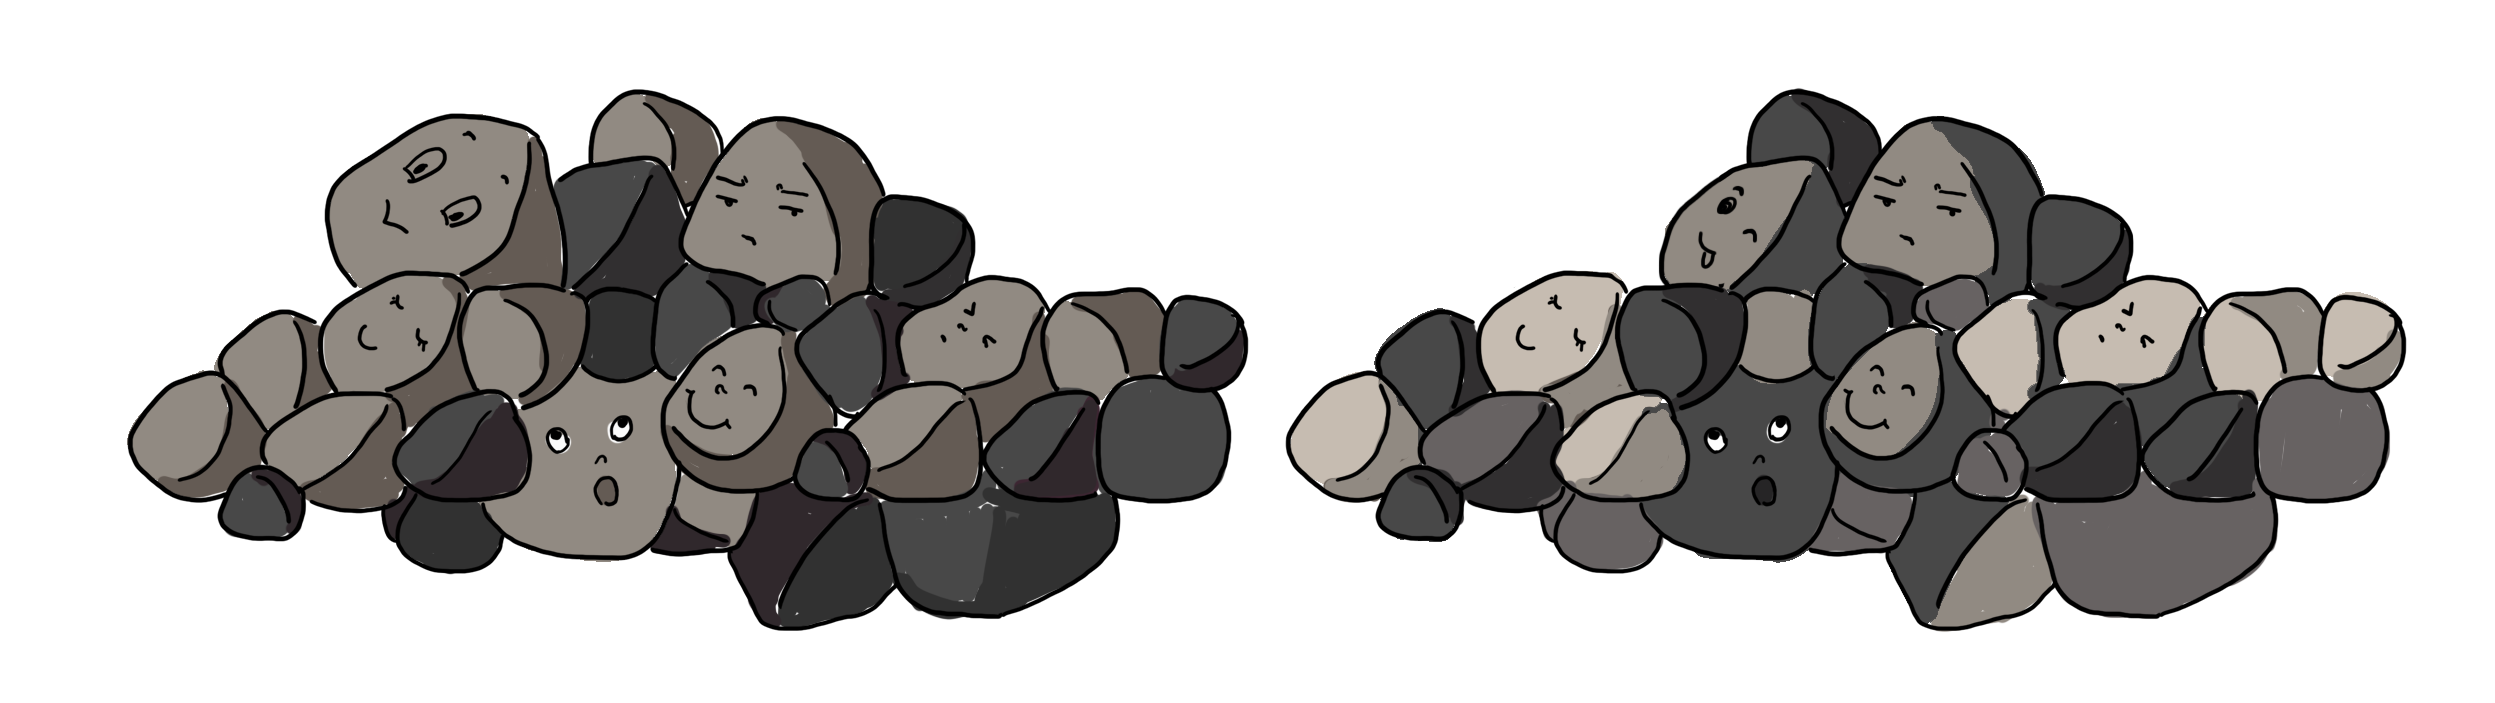
\includegraphics[width=1\linewidth]{bai5}
		\vspace*{-15pt}
	\end{figure}
	\textit{Lời giải.} 	Ta nhận thấy sau mỗi một bước, số đá trên bàn giảm đi $1$ viên nhưng số đống đá lại tăng thêm $1$. Vì vậy tổng số các viên đá và số các đống đá ở trên bàn không thay đổi sau mỗi lần nhặt bớt đi viên đá. Ban đầu tổng số này là $1001+1=1002$ không chia hết cho $4$. Vì thế, ta không thể nhận được tình huống khi trên bàn chỉ còn toàn các đống đá, mỗi đống có đúng $3$ viên, vì khi đó tổng số này sẽ bằng $3k+k=4k$ (chia hết cho $4$), ở đó $k$ là số các đống đá lúc đó ở trên mặt bàn. 
	\vskip 0.1cm
 	$\pmb{6.}$ Thạch Sanh chuẩn bị lên đường tiêu diệt Mãng xà -- con quái vật có tận $3$ cái đầu và $3$ cái đuôi gớm ghiếc. Ngài Thần Miếu đưa cho chàng một bảo bối và dặn dò: ``Đây là chiếc gươm thần thiêng liêng. Bằng một nhát gươm, con có thể chém đứt được một cái đầu, hoặc là hai cái đầu, hoặc là một cái đuôi, hoặc là hai cái đuôi của con Mãng xà. Nhưng con nên nhớ, nếu con chỉ chém đứt một cái đầu, thì một cái đầu khác của nó sẽ mọc lên, nếu chỉ chém đứt một cái đuôi, thì hai cái đuôi khác lại mọc ra, nếu chém đứt hai cái đuôi thì một cái đầu khác lại mọc ra, còn nếu con chém đứt được hai cái đầu thì không có gì mọc ra thêm nữa". Vậy Thạch Sanh có thể chém đứt tất cả đầu và đuôi của con Mãng xà sau bao nhiêu nhát gươm?
	\begin{figure}[H]
		\centering
		\vspace*{-5pt}
		\captionsetup{labelformat= empty, justification=centering}
		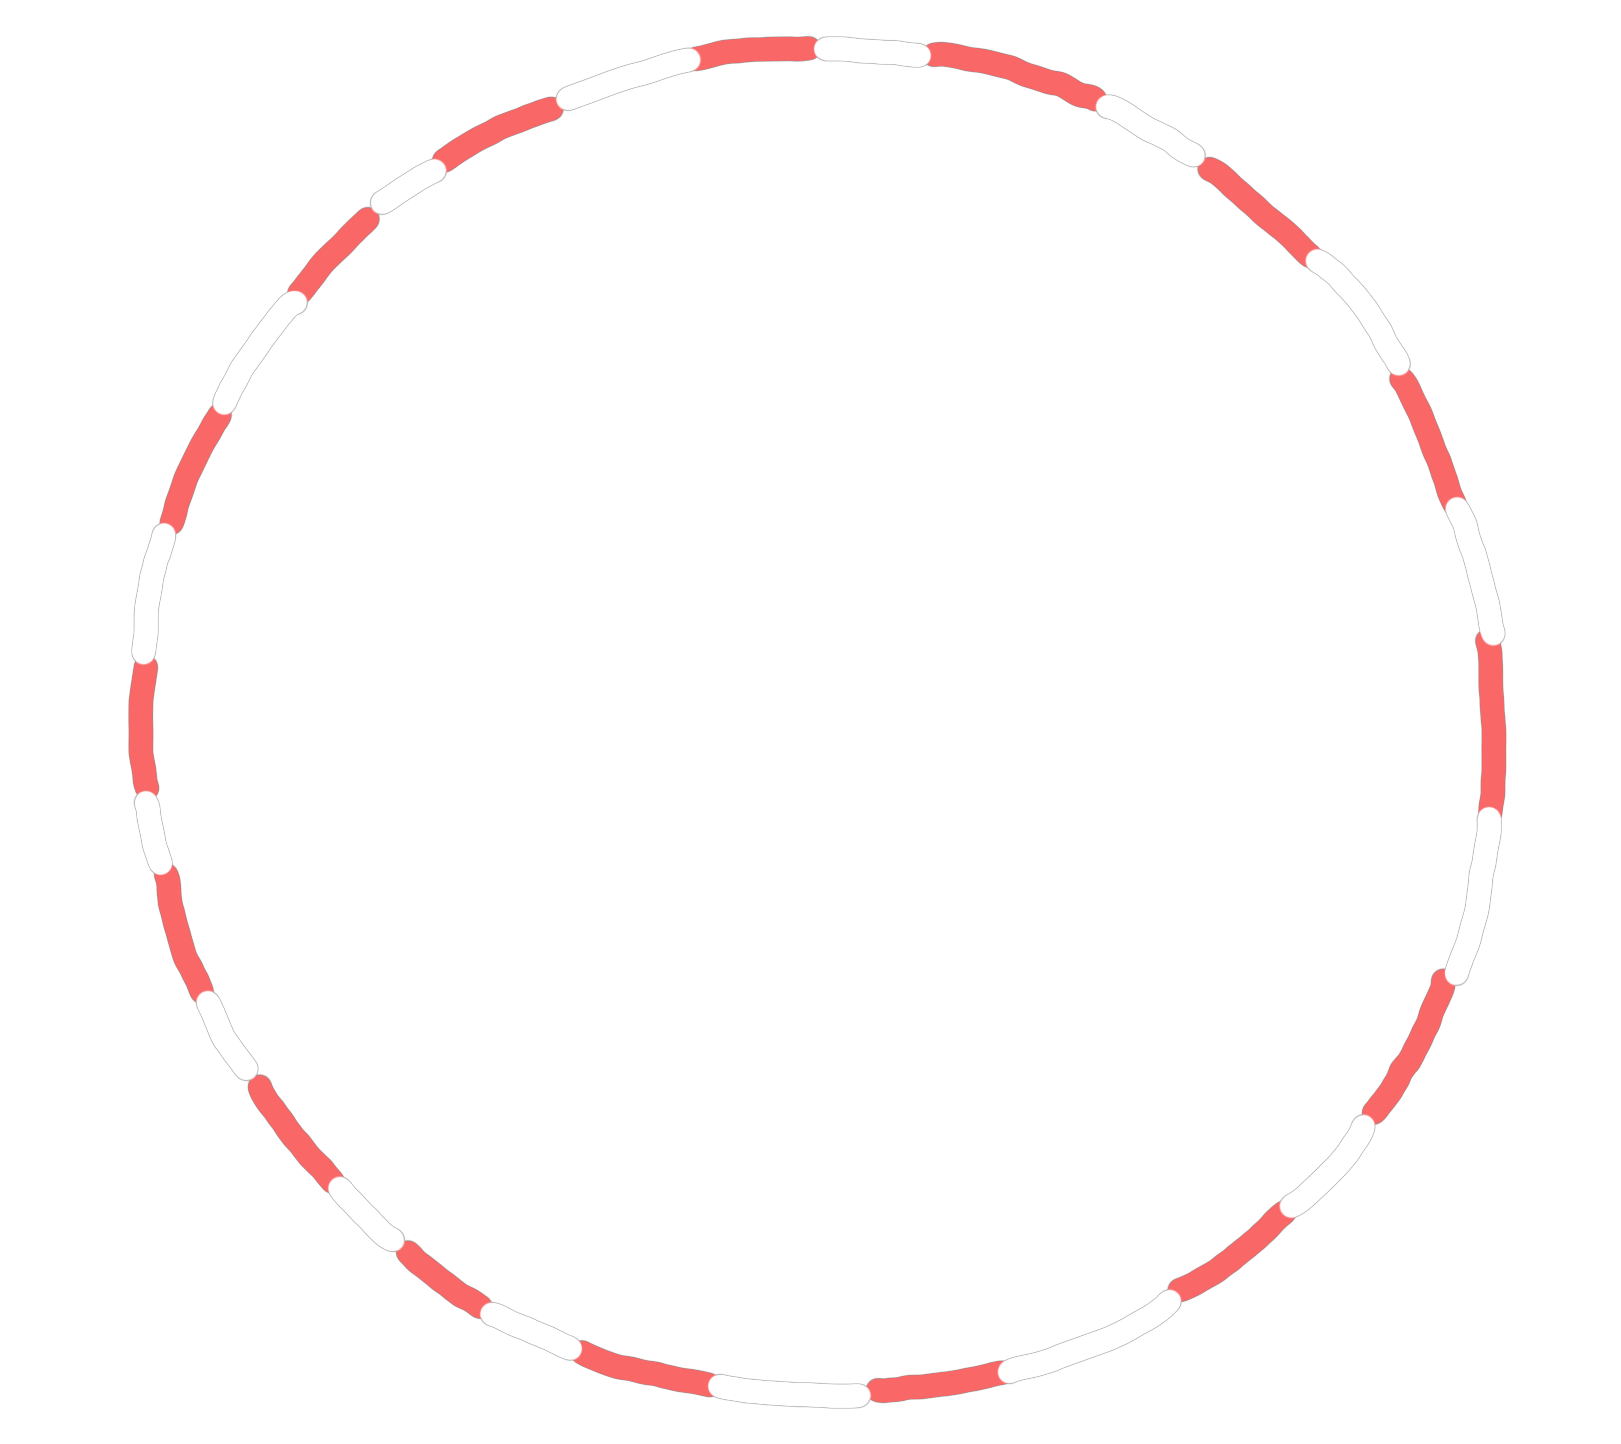
\includegraphics[width=1\linewidth]{bai6}
		\vspace*{-5pt}
	\end{figure}
	\textit{Lời giải.} Để chiến thắng được Mãng xà, Thạch Sanh phải chém đứt được một số chẵn cái đầu của nó. Số đầu mới của Mãng xà sẽ tăng thêm chỉ trong trường hợp nếu Thạch Sanh chém đứt một số cái đuôi nào của con  chằn tinh này. Do có tất cả $3$ cái đuôi, nên nếu chém đứt tất cả đuôi của Mãng xà, thì số đầu mới mọc ra không ít hơn  $2$ cái. Vì thế tổng số đầu mà Thạch Sanh cần phải chém để thắng không ít hơn $5$ cái. Do vậy, một số chẵn cái đầu cần chém đứt phải tối thiểu là $6$ cái. Đây là cách Thạch Sanh tiêu diệt Mãng xà với $6$ đầu: Đầu tiên, chàng sẽ lần lượt chặt đứt từng cái đuôi (với $3$ nhát gươm). Mãng xà giờ có $6$ đuôi mới và $3$ đầu. Sau đó chàng lần lượt sẽ chặt đứt từng cặp đuôi (với $3$ nhát gươm). Lúc này Mãng xà giờ có $6$ đầu và $0$ đuôi. Cuối cùng Thạch Sanh sẽ lần lượt chặt từng cặp $2$ cái đầu sau $3$ nhát chém. Tóm lại, với $9$ nhát gươm Thạch Sanh sẽ hạ được con chằn tinh.
\end{multicols}
\newpage
\begingroup
\thispagestyle{toancuabinone}
\blfootnote{$^1$\color{toancuabi}Canada.}
\AddToShipoutPicture*{\put(60,733){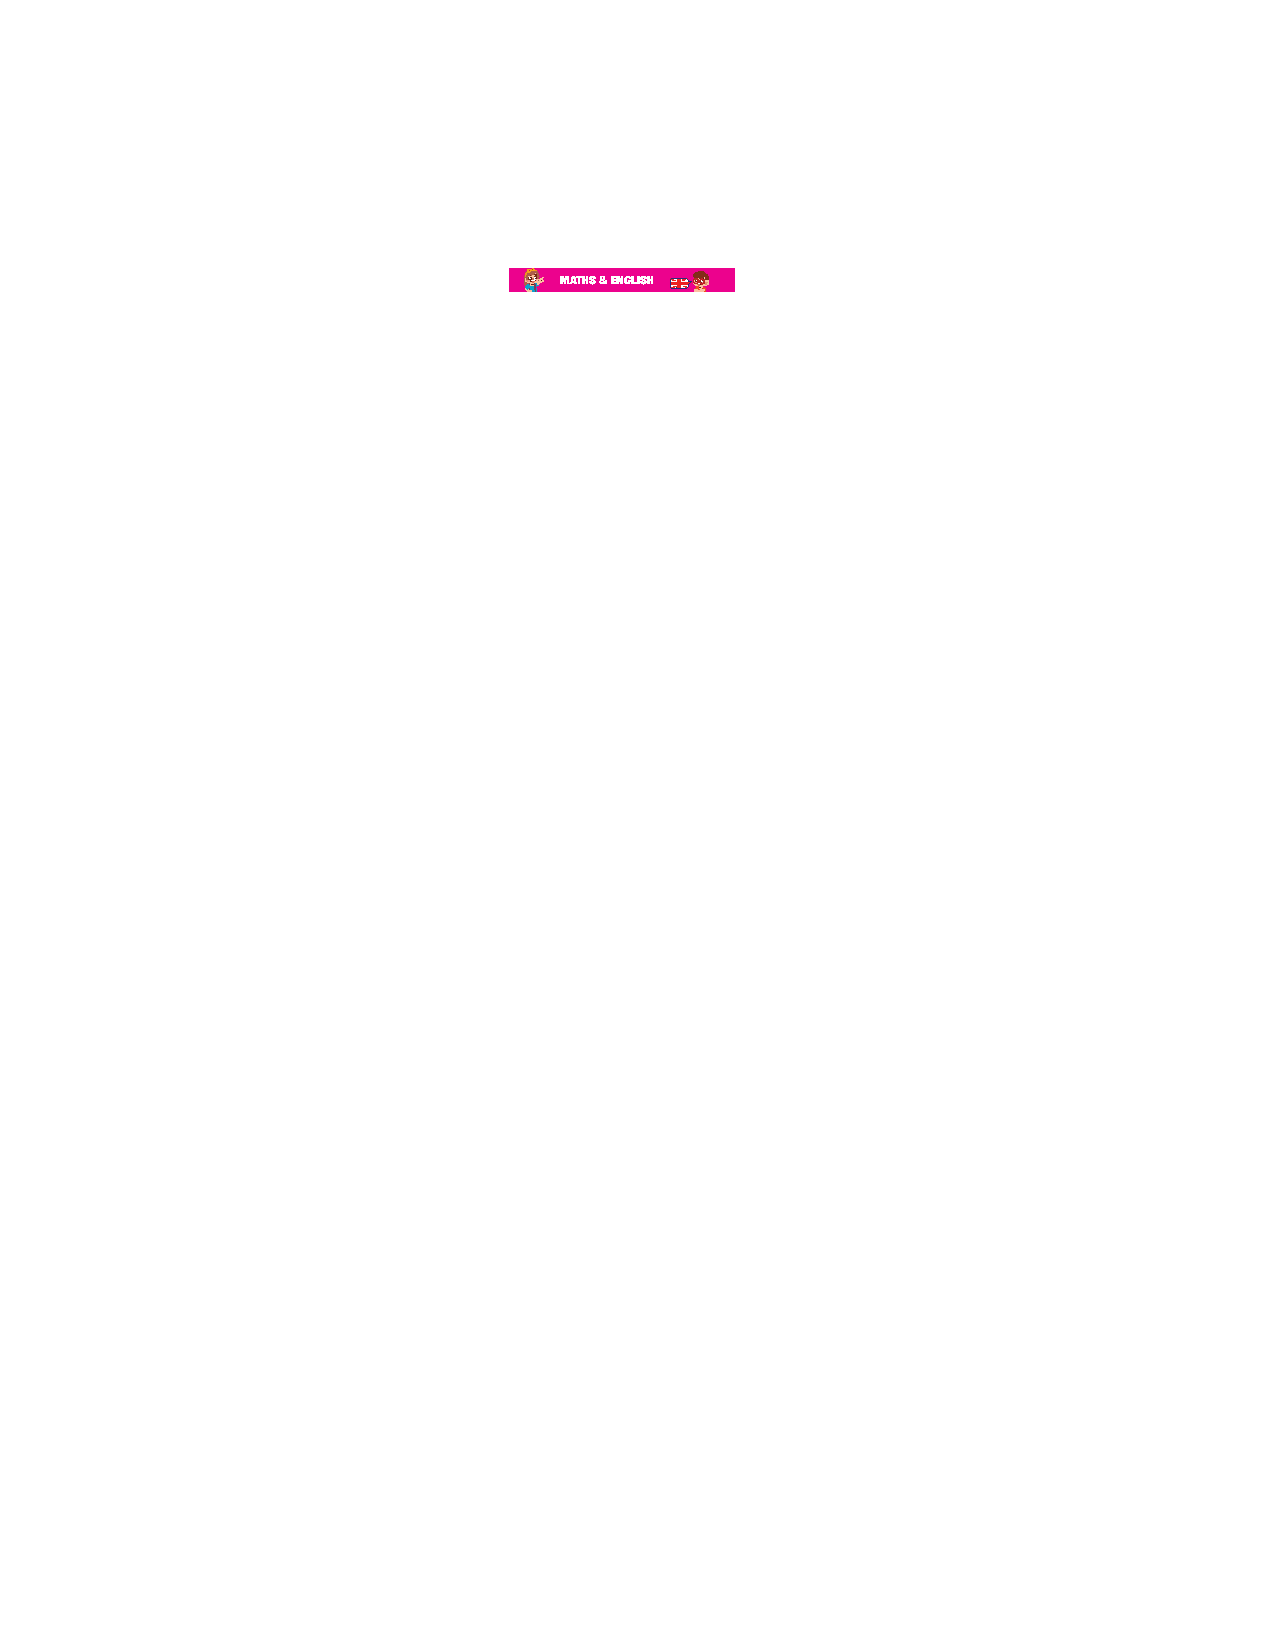
\includegraphics[width=17.2cm]{../mathc.pdf}}}
%\AddToShipoutPicture*{\put(-2,733){
\includegraphics[width=17.2cm]{../mathl.pdf}}} 
\AddToShipoutPicture*{\put(88,675){
\includegraphics[scale=1]{../tieude3.pdf}}} 
\centering
\endgroup
\graphicspath{{../toancuabi/pic/}}
\vspace*{35pt}

\begin{multicols}{2}
	Usually approaching a problem from different angles help to see different nature of the problem,
	more importantly of what we learned, and how to apply them.
	In this article, we shows five different approaches, or solutions, to a simple geometry problem.
	\vskip 0.2cm
	\PIbox{\textbf{\color{toancuabi}Example}
	\vskip 0.1cm
	Let $ABCD$ be a square, $E$ is the midpoint of side $AD,$
	and $F$ is the foot of the altitude from $C$ to $BE.$
	Prove that $DF = DA.$}
	\begin{figure}[H]
		\vspace*{-5pt}
		\centering
		\captionsetup{labelformat= empty, justification=centering}
		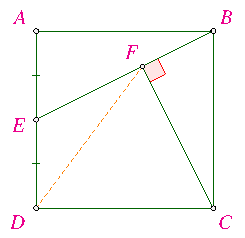
\includegraphics[width= 0.7\linewidth]{2022-2-ms-1-1.pdf}
		\vspace*{-15pt}
	\end{figure}
	\textit{First proof -- Using congruent triangles}.
	Extending $FE$ to intersect $CD$ at $G,$ see the diagram on the left. 
	Since $\angle AEB = \angle GED, AE = ED, \angle EAB = \angle EDA = 90^\circ,$
	by the angle-side-angle (ASA) rule, the triangles $ EAB$ and $EDG,$ are equal,
	thus the corresponding pair of sides are the same, or $DG=AB$. Therefore $DG=DC.$
	\begin{figure}[H]
		\vspace*{-5pt}
		\centering
		\captionsetup{labelformat= empty, justification=centering}
		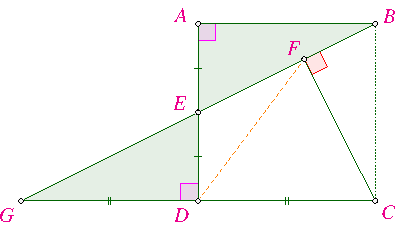
\includegraphics[width= 1\linewidth]{2022-2-ms-1-1-a.pdf}
		\vspace*{-15pt}
	\end{figure}
	\begin{figure}[H]
		\vspace*{-5pt}
		\centering
		\captionsetup{labelformat= empty, justification=centering}
		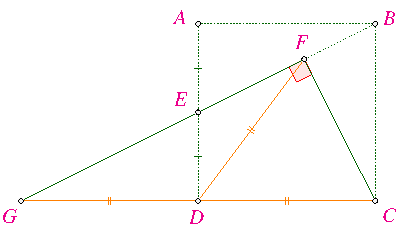
\includegraphics[width= 1\linewidth]{2022-2-ms-1-1-b.pdf}
		\vspace*{-15pt}
	\end{figure}	
	Now, it is a well--known fact that,
	\textit{the midpoint of the hypotenuse of a right triangle is at equidistance from all vertices.}
	Using this fact for $\triangle DGC$ in the diagram on the right in the figure above, $DG=DC,\ \angle{GFC} = 90^\circ,$ thus $DF=DG=DC.$
	\vskip 0.1cm
	\textit{Second proof -- Using median segment.}
	Let $G$ be the midpoint of $BC,$ and let $DG$ intersect $FC$ at $H.$
	By side--side--side (SSS) rule, the triangle $ EAB$ and $  GCD$ are equal,
	so $\angle ABE = \angle CDG$, implying $EB \parallel DG.$
	\begin{figure}[H]
		\vspace*{-15pt}
		\centering
		\captionsetup{labelformat= empty, justification=centering}
		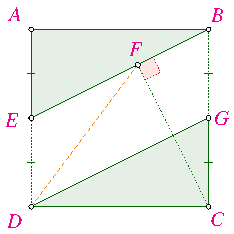
\includegraphics[width= 0.7\linewidth]{2022-2-ms-1-1-c.pdf}
		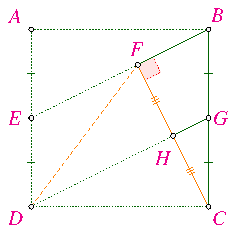
\includegraphics[width= 0.7\linewidth]{2022-2-ms-1-1-d.pdf}
		\vspace*{-5pt}
	\end{figure}	
	Furthermore, in $\triangle FBC,$ $GH \parallel BF,$ $G$ is midpoint of $BC,$
	so $H$ is midpoint of $FC.$
	Finally, in $\triangle DFC,$ $DH \perp FC,$ $H$ is midpoint of $FC,$
	thus by side--angle--side (SAS) rule, the triangles $ DHF$ and $DHC$ are equal, hence $DF = DC.$
	\begin{figure}[H]
		\vspace*{-10pt}
		\centering
		\captionsetup{labelformat= empty, justification=centering}
		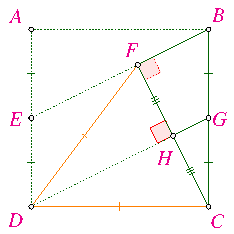
\includegraphics[width= 0.7\linewidth]{2022-2-ms-1-1-e.pdf}
		\vspace*{-15pt}
	\end{figure}		
	\textit{Third proof -- Using angles in circle}.
	The triangles $EDC$ and $ EFC$ are right at $D$ and $F.$ respectively. It follows that the points $C, D, E,$ and $F$ are on the circle centered at $G.$
	\begin{figure}[H]
		\vspace*{-15pt}
		\centering
		\captionsetup{labelformat= empty, justification=centering}
		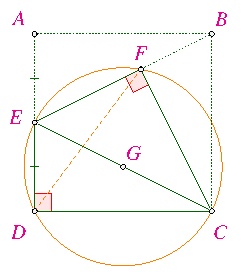
\includegraphics[width= 0.7\linewidth]{2022-2-ms-1-1-f.pdf}
		\captionsetup{labelformat= empty, justification=centering}
		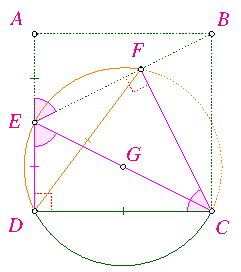
\includegraphics[width= 0.7\linewidth]{2022-2-ms-1-1-g.pdf}
		\vspace*{-5pt}
	\end{figure}	
	$\angle DEC = \angle AEB = 180^{\circ} - \angle DEF = \angle DCF.$ 
	$\angle DEC = \angle DFC$ (subtends arc $DC$).
	$\angle DCF = \angle DFC$, $\triangle DCF$ is isosceles, thus $DC = DF.$
	\vskip 0.1cm
	\textit{Fourth proof -- Using triangle trigonometry}.
	First, by Pythagorean theorem, $EB = \sqrt{AB^2 +AE^2} = \frac{a\sqrt{5}}{2}.$
	Then, let $\alpha = \angle DCF = \angle FBC = \angle AEB.$
	It is easy to see that $\cos{\alpha} = \frac{AE}{EB} = \frac{1}{\sqrt{5}},$
	and since $\triangle FCB \sim \triangle ABE$, $\frac{FC}{BC} = \sin{\alpha} = \frac{AB}{EB} = \frac{2}{\sqrt{5}},$
	so $FC = BC \sin{\alpha} = \frac{2a}{\sqrt{5}}.$
	\begin{figure}[H]
		\vspace*{-10pt}
		\centering
		\captionsetup{labelformat= empty, justification=centering}
		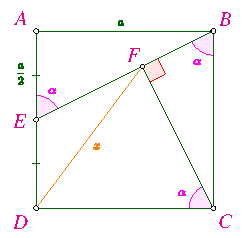
\includegraphics[width= 0.7\linewidth]{2022-2-ms-1-1-h.pdf}
		\vspace*{-15pt}
	\end{figure}	
	By the Law of Cosines,
	\begin{align*}
		DF &= \sqrt{DC^2 +  FC^2 - 2(DC)(FC)\cos{\alpha}}\\
		&= \sqrt{a^2 + \left(\frac{2a}{\sqrt{5}}\right)^2 - 2a \frac{2a}{\sqrt{5}} \frac{1}{\sqrt{5}}} = a.
	\end{align*}
	\textit{Fifth proof -- Using Ptolemy theorem}.
	Similar to the previous proof,
	let $DC = a \Rightarrow EB = EC = \frac{a\sqrt{5}}{2}.$ 
	$\frac{FC}{BC} = \frac{AB}{EB} \Rightarrow FC=\frac{2a}{\sqrt{5}}.$
	$\frac{FB}{BC} = \frac{AE}{EB} \Rightarrow FB=\frac{a}{\sqrt{5}}.$
	\begin{figure}[H]
		\vspace*{-15pt}
		\centering
		\captionsetup{labelformat= empty, justification=centering}
		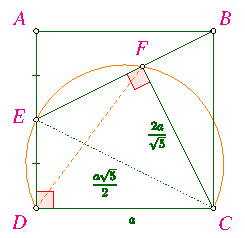
\includegraphics[width= 0.7\linewidth]{2022-2-ms-1-1-i.pdf}
		\vspace*{-15pt}
	\end{figure}	
	By Ptolemy theorem for the cyclic quadrilateral $CDEF,$
	$DF \cdot EC = ED \cdot FC + EF \cdot DC 
	= \frac{a}{2}\cdot \frac{2a}{\sqrt{5}} + \left(\frac{a\sqrt{5}}{2} - \frac{a}{\sqrt{5}} \right) \cdot a
	= \frac{a^2\sqrt{5}}{2} \Rightarrow DF = a.$
	\vskip 0.1cm
	Be open minded. Look for alternative approach. Try to use your own toolbox before looking for something else.
	Often you know more than you think you know.
\end{multicols}
%	\newpage
	
%	\setcounter{figure}{0}
%	\thispagestyle{thachthuctoanhocnone}
\pagestyle{thachthuctoanhoc}
\everymath{\color{thachthuctoanhoc}}
\graphicspath{{../thachthuctoanhoc/pic/}}
\begingroup
\AddToShipoutPicture*{\put(0,616){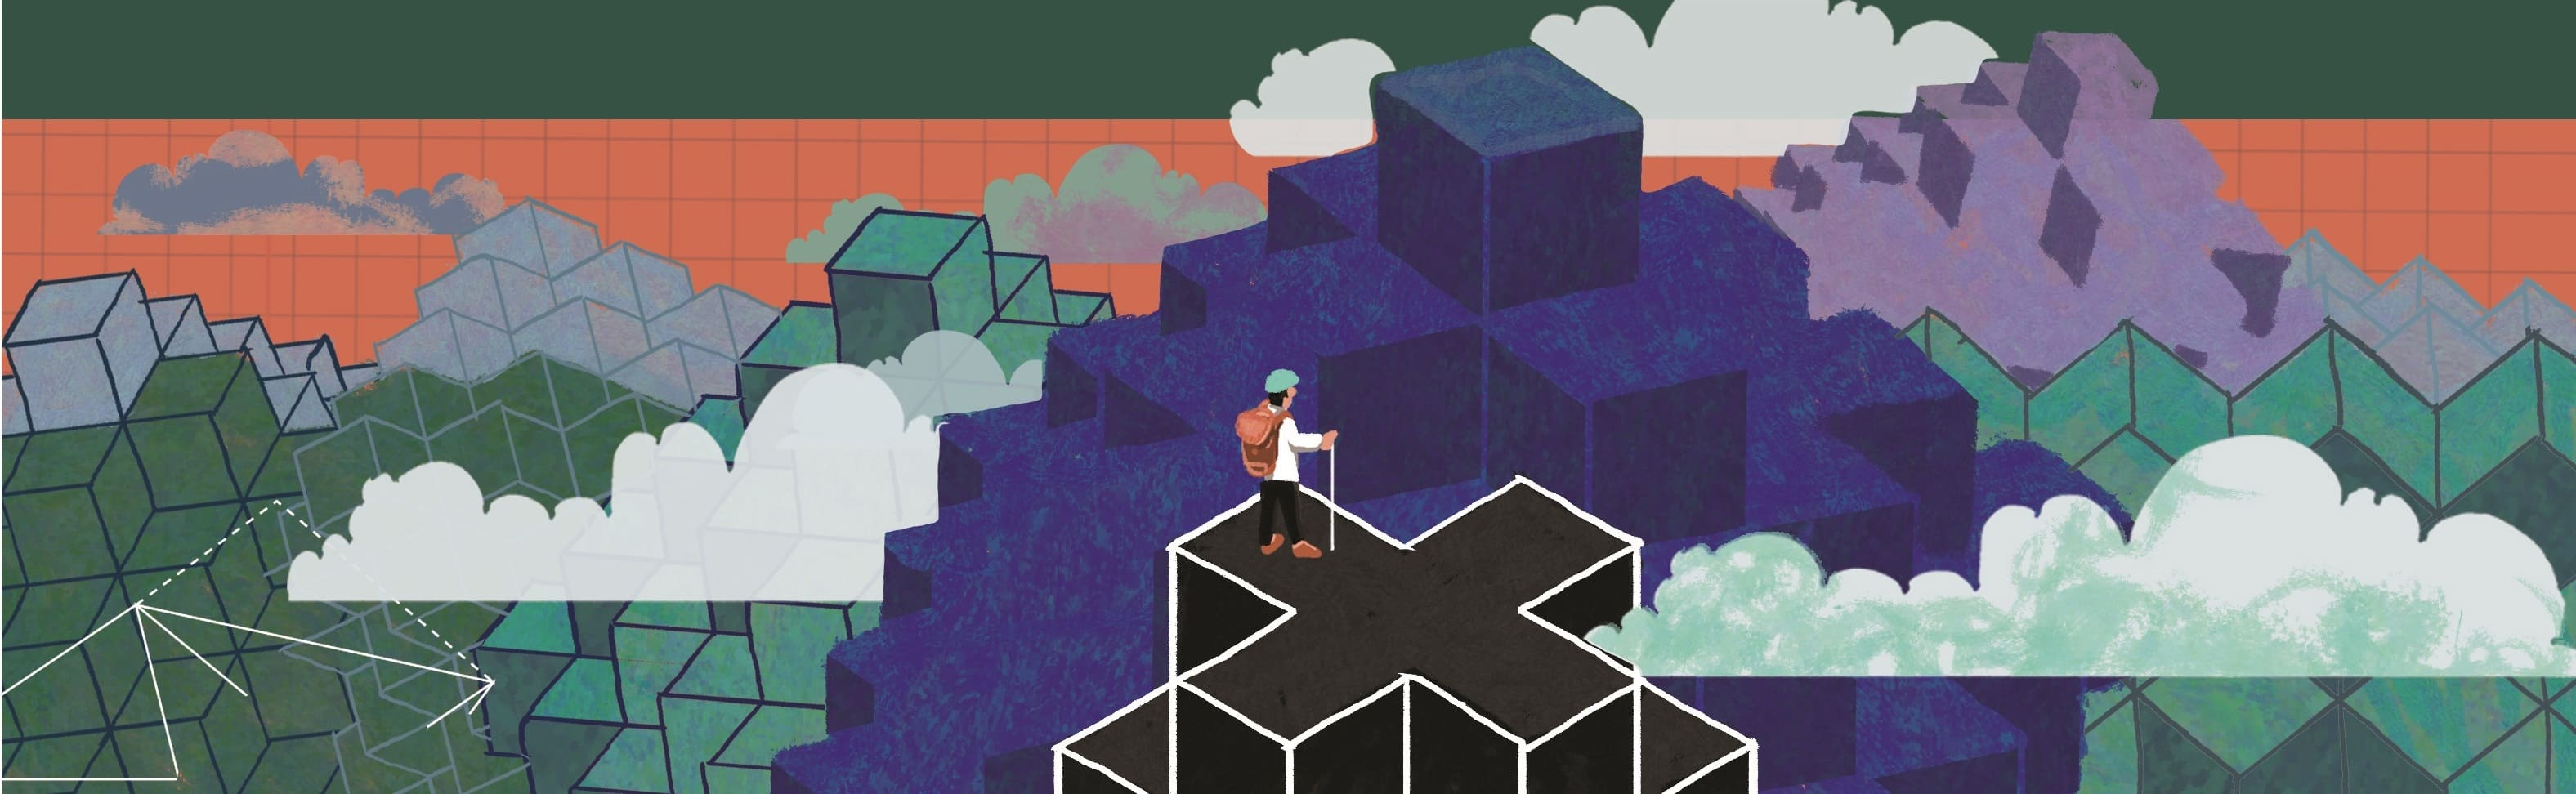
\includegraphics[width=19.3cm]{../thachthuctoanhoc/bannerthachthuc}}}
\centering
\vspace*{4cm}
\endgroup
\vspace*{-8pt}
\begin{tBox}
	\begin{itemize}[leftmargin = 13pt, itemsep = 1.0pt] 
		\item Mỗi bài toán đề xuất (kèm theo lời giải) cần được nêu rõ là bài sáng tác hay bài sưu tầm.
%		\item Mỗi bài toán đề xuất (kèm theo lời giải) cần được nêu rõ là bài sáng tác hay bài sưu tầm (nếu là bài sưu tầm, cần ghi rõ nguồn).
		\item Bài giải cho mỗi bài toán cần được trình bày trong một file riêng hoặc
		một tờ giấy riêng.
		\item  Người đề xuất bài toán hoặc gửi bài giải cho các bài toán trong mục ``Thách thức kỳ này" cần ghi rõ họ, đệm, tên và nơi làm việc/học tập, số điện thoại liên hệ. Nếu là học sinh (hoặc sinh viên) cần ghi rõ là học sinh lớp mấy (hoặc sinh viên năm thứ mấy).
		\item Các bài toán trong mục Thách thức kỳ này hướng tới các độc giả là học sinh phổ thông; được phân chia thành các mức độ $B$, $A$, và được sắp xếp theo độ khó tăng dần, theo đánh giá chủ quan của Ban biên tập. Các bài toán mức độ $B$ không đòi hỏi các kiến thức vượt quá chương trình môn Toán cấp THCS; các bài toán mức độ $A$ không đòi hỏi các kiến thức vượt quá chương trình môn Toán cấp THPT.
		\item Cách thức gửi bài toán đề xuất hoặc lời giải: gửi file thu được bằng cách scan, ảnh chụp (rõ nét) của bản viết tay, hoặc được soạn thảo bằng các phần mềm Latex, Word tới \url{bbt@pi.edu.vn} hoặc gửi qua đường bưu điện tới Tòa soạn (xem địa chỉ tại bìa $2$).
		\item Hạn gửi lời giải cho các bài toán P$651$--P$660$: trước ngày $15/12/2022$.
	\end{itemize}
\end{tBox}
%\begin{center}
%	\vspace*{-5pt}
%	\textbf{\color{thachthuctoanhoc}\color{thachthuctoanhoc}\color{thachthuctoanhoc}THÁCH THỨC KỲ NÀY}
%	\vspace*{-5pt}
%\end{center}
%\begin{multicols}{2}
%	\setlength{\abovedisplayskip}{4pt}
%	\setlength{\belowdisplayskip}{4pt}
%	{\color{thachthuctoanhoc}{\usefont{T5}{qag}{b}{n} P651.}}
%	(Mức $B$) Trong một hộp chứa $2$ loại bi: bi đỏ và bi xanh. Số bi đỏ chiếm $\dfrac4{15}$ số lượng bi. Sau khi người ta đổ thêm một túi gồm $200$ bi, thì số lượng bi đỏ chiếm $\dfrac{11}{25}$. Hỏi số lượng bi đỏ khi đó ít nhất là bao nhiêu?
%	\begin{flushright}
%		\textit{Đăng Hải, Hà Nội}
%	\end{flushright}
%	{\color{thachthuctoanhoc}{\usefont{T5}{qag}{b}{n} P652.}}
%	(Mức $B$) Xét các số nguyên dương $a,b$. Hãy tìm điều kiện cần và đủ của $a,b$ để tồn tại số nguyên dương $c$ sao cho $a^2\!+\!b^2\!+\!c^2$ là một số chính phương.
%	\begin{flushright}
%		\textit{Nguyễn Đức Tấn, Tp. Hồ Chí Minh}
%	\end{flushright}
%	{\color{thachthuctoanhoc}{\usefont{T5}{qag}{b}{n} P653.}}
%	(Mức $B$) Cho hình chữ nhật $ABCD$. Gọi $E$ là hình chiếu vuông góc của điểm $B$ trên đường thẳng $AC$; $F$ là trung điểm của đoạn $AE$. Các đường thẳng $BF,$ $AD$ cắt nhau tại $G$. Gọi $K$ là trung điểm của $AG$. Chứng minh rằng $DK+KF>CF$.
%	\begin{center}
%		\definecolor{qqwuqq}{rgb}{0,0.39215686274509803,0}
%		\definecolor{ffqqqq}{rgb}{1,0,0}
%		\definecolor{qqzzff}{rgb}{0,0.6,1}
%		\definecolor{qqqqff}{rgb}{0,0,1}
%		\definecolor{qqqqffa}{rgb}{1,1,1}
%		\begin{tikzpicture}[line cap=round,line join=round,>=triangle 45,x=1cm,y=1cm]
%			\draw[,color=qqwuqq] (0.5120224474090631,0.5610443487905639) -- (0.20582785007023013,0.7378065295886914) -- (0.029065669272102523,0.4316119322498584) -- (0.33526026661093555,0.2548497514517308) -- cycle; 
%			\draw [,color=qqzzff] (-4.42,3)-- (1.92,3);
%			\draw [,color=qqzzff] (-4.42,-0.66)-- (1.92,-0.66);
%			\draw [,color=qqzzff] (1.92,-0.66)-- (1.92,3);
%			\draw [] (-4.42,3)-- (1.92,-0.66);
%			\draw [] (-4.42,1.9019038377710236)-- (-2.042369866694532,1.6274248757258654);
%			\draw [] (-4.42,0.8038076755420471)-- (1.92,3);
%			\draw [,color=ffqqqq] (1.92,3)-- (0.33526026661093555,0.2548497514517308);
%			\draw [] (-4.42,3)-- (-2.042369866694532,1.6274248757258654);
%			\draw [] (-3.1861886281353815,2.391656857273683) -- (-3.276181238559151,2.235768018452182);
%			\draw [] (-2.042369866694532,1.6274248757258654)-- (0.33526026661093555,0.2548497514517308);
%			\draw [] (-0.8085584948299132,1.0190817329995472) -- (-0.8985511052536825,0.8631928941780476);
%			\draw [,color=qqzzff] (-4.42,3)-- (-4.42,1.9019038377710236);
%			\draw [,color=qqzzff] (-4.32,2.4909519188855116) -- (-4.52,2.4909519188855116);
%			\draw [,color=qqzzff] (-4.32,2.4109519188855115) -- (-4.52,2.4109519188855115);
%			\draw [,color=qqzzff] (-4.42,1.9019038377710236)-- (-4.42,0.8038076755420471);
%			\draw [,color=qqzzff] (-4.32,1.3928557566565354) -- (-4.52,1.3928557566565354);
%			\draw [,color=qqzzff] (-4.32,1.3128557566565353) -- (-4.52,1.3128557566565353);
%			\draw [,color=qqzzff] (-4.42,0.8038076755420471)-- (-4.42,-0.66);
%			\draw [fill=qqqqffa] (-4.42,3) circle (1.6pt);
%			\draw[color=qqqqff] (-4.54,3.45) node {$A$};
%			\draw [fill=qqqqffa] (1.92,3) circle (1.6pt);
%			\draw[color=qqqqff] (1.94,3.51) node {$B$};
%			\draw [fill=qqqqffa] (1.92,-0.66) circle (1.6pt);
%			\draw[color=qqqqff] (1.96,-0.95) node {$C$};
%			\draw [fill=qqqqffa] (-4.42,-0.66) circle (1.6pt);
%			\draw[color=qqqqff] (-4.54,-0.93) node {$D$};
%			\draw [fill=qqqqffa] (0.33526026661093555,0.2548497514517308) circle (1.6pt);
%			\draw[color=qqqqff] (0.12,0.07) node {$E$};
%			\draw [fill=qqqqffa] (-2.042369866694532,1.6274248757258654) circle (1.6pt);
%			\draw[color=qqqqff] (-2,2.07) node {$F$};
%			\draw [fill=qqqqffa] (-4.42,0.8038076755420471) circle (1.6pt);
%			\draw[color=qqqqff] (-4.74,0.93) node {$G$};
%			\draw [fill=qqqqffa] (-4.42,1.9019038377710236) circle (1.6pt);
%			\draw[color=qqqqff] (-4.74,1.95) node {$K$};
%		\end{tikzpicture}
%	\end{center}
%	\begin{flushright}
%		\textit{Trần Thanh Hưng, Phú Yên}
%	\end{flushright}
%	{\color{thachthuctoanhoc}{\usefont{T5}{qag}{b}{n} P654.}}
%	(Mức $B$) Xét hàm số $f(x)=2x^3-3x^2+4x-5$. Tính tổng
%	\begin{align*}
%		S=&f\left(\dfrac1{2023}\right)+f\left(\dfrac2{2023}\right)+f\left(\dfrac3{2023}\right)\\
%		&+\cdots+f\left(\dfrac{2022}{2023}\right).
%	\end{align*}
%	\begin{flushright}
%		\textit{Nguyễn Tường Thanh, Nghệ An}
%	\end{flushright}
%	{\color{thachthuctoanhoc}{\usefont{T5}{qag}{b}{n} P655.}}
%	(Mức $B$) Tại mỗi đỉnh của một đa giác đều $2023$ cạnh, người ta ghi một số thực sao cho các số được ghi là đôi một khác nhau. Chứng minh rằng, có thể tìm được một tam giác $ABC$ cân tại $A$, với $A,B,C$ là các đỉnh của đa giác lồi đã cho và sao cho số được ghi tại đỉnh $A$ nằm giữa hai số được ghi tại đỉnh $B$ và $C$. 
%	\begin{flushright}
%		\textit{Lưu Tiến Đức, Hà Nội}
%	\end{flushright}
%	{\color{thachthuctoanhoc}{\usefont{T5}{qag}{b}{n} P656.}}
%	(Mức $B$) Xét $2022$ số thực $x_1\leq x_2\leq \cdots\leq x_{2022}$ thoả mãn: tổng các số dương bằng $\dfrac12$ và tổng các số âm bằng $-\dfrac12$. Tìm giá trị lớn nhất có thể của $M=x_{999}-x_{32}$. 
%	\begin{flushright}
%		\textit{Bằng Linh, Phú Thọ (st)}
%	\end{flushright}
%	{\color{thachthuctoanhoc}{\usefont{T5}{qag}{b}{n} P657.}}
%	(Mức $A$) Cho $a,b$ là các số thực phân biệt thuộc đoạn $[0;\pi]$ và thoả mãn $e^a\cdot\sin a=e^b\cdot\sin b$. Chứng minh rằng, \linebreak$\pi\leq a+b\leq \dfrac{3\pi}2$. 
%	\begin{flushright}
%		\textit{Trần Quốc Luật, Tp. Hồ Chí Minh}
%	\end{flushright}
%	{\color{thachthuctoanhoc}{\usefont{T5}{qag}{b}{n} P658.}}
%	(Mức $A$) Cho số nguyên dương $n$. Giả sử $P(x)$ là một đa thức hệ số thực, có bậc nhỏ hơn $n$ sao cho đa thức $Q(x)=x^n\cdot P(x)+1$ nhận $x=2022$ là một nghiệm, với bội không nhỏ hơn $n$. Tính giá trị của $P(1011)$.
%	\begin{flushright}
%		\textit{Duy Minh, Hà Nội}
%	\end{flushright}
%	{\color{thachthuctoanhoc}{\usefont{T5}{qag}{b}{n} P659.}}
%	(Mức $A$) Cho tam giác $A B C$ cân tại $A$. Lấy điểm $P$ bất kì trên cạnh $B C$ ($P$ khác $B$, $C$ và trung điểm $BC$). Kẻ các đường thẳng $m$ và $n$  đi qua $P$ và đối xứng nhau qua đường thẳng $BC$. Đường thẳng $m$ cắt các đường thẳng $A B$, $A C$ lần lượt tại $E$, $N$. Đường thẳng $n$ cắt các đường thẳng $A C$, $A B$ lần lượt tại $F$, $M$. Chứng minh rằng, đường tròn ngoại tiếp tam giác tạo bởi ba đường thẳng cắt nhau $B C$,  $M N$, $E F$ tiếp xúc với đường tròn ngoại tiếp tam giác $A B C$.
%	\begin{center}
%		\definecolor{xfqqff}{rgb}{0.4980392156862745,0,1}
%		\definecolor{ffqqqq}{rgb}{1,0,0}
%		\definecolor{qqzzff}{rgb}{0,0.6,1}
%		\definecolor{qqqqff}{rgb}{0,0,1}
%		\definecolor{qqqqffa}{rgb}{1,1,1}
%		\begin{tikzpicture}[thick, scale=0.5, every node/.style={scale=0.9}, line cap=round,line join=round,>=triangle 45,x=1cm,y=1cm]
%			\draw [,color=qqzzff] (-2,-1.8)-- (3,-1.8);
%			\draw [,color=qqzzff] (-2,-1.8)-- (0.5,4.7);
%			\draw [,color=qqzzff] (0.5,4.7)-- (3,-1.8);
%			\draw [,color=qqzzff] (-3.335284691878354,-5.27174019888372)-- (-2,-1.8);
%			\draw [] (-1.2373124800510693,0.18298755186721993)-- (3.5416215015249546,-3.208215903964881);
%			\draw [,color=qqzzff] (3.5416215015249546,-3.208215903964881)-- (3,-1.8);
%			\draw [] (2.6906367890970206,-0.9956556516522528)-- (-3.335284691878354,-5.27174019888372);
%			\draw [,color=ffqqqq] (0.5,0.9692307692307693) circle (3.730769230769231cm);
%			\draw [dashed,color=xfqqff] (6.802921043005886,0.3708782072039446) circle (2.600489685342991cm);
%			\draw [] (-1.2373124800510693,0.18298755186721993)-- (6.8029210430058855,-2.2296114781390464);
%			\draw [,color=qqzzff] (8.234645322698828,-1.8)-- (3,-1.8);
%			\draw [] (8.234645322698828,-1.8)-- (-3.335284691878354,-5.27174019888372);
%			\draw [fill=qqqqffa] (-2,-1.8) circle (1.6pt);
%			\draw[color=qqqqff] (-2.52,-1.9) node {$B$};
%			\draw [fill=qqqqffa] (3,-1.8) circle (1.6pt);
%			\draw[color=qqqqff] (3.65,-2.2) node {$C$};
%			\draw [fill=qqqqffa] (0.5,4.7) circle (1.6pt);
%			\draw[color=qqqqff] (0.48,5.17) node {$A$};
%			\draw [fill=qqqqffa] (1.5571428571428578,-1.8) circle (1.6pt);
%			\draw[color=qqqqff] (1.52,-2.35) node {$P$};
%			\draw [fill=qqqqffa] (-1.2373124800510693,0.18298755186721993) circle (1.6pt);
%			\draw[color=qqqqff] (-1.56,0.49) node {$E$};
%			\draw [fill=qqqqffa] (2.6906367890970206,-0.9956556516522528) circle (1.6pt);
%			\draw[color=qqqqff] (3.02,-0.65) node {$F$};
%			\draw [fill=qqqqffa] (-3.335284691878354,-5.27174019888372) circle (1.6pt);
%			\draw[color=qqqqff] (-3.9,-5.49) node {$M$};
%			\draw [fill=qqqqffa] (3.5416215015249546,-3.208215903964881) circle (1.6pt);
%			\draw[color=qqqqff] (3.54,-3.8) node {$N$};
%			\draw [fill=qqqqffa] (5.371196763312944,-1.8) circle (1.6pt);
%			\draw [fill=qqqqffa] (6.8029210430058855,-2.2296114781390464) circle (1.6pt);
%			\draw [fill=qqqqffa] (8.234645322698828,-1.8) circle (1.6pt);
%		\end{tikzpicture}
%	\end{center}
%	\begin{flushright}
%		\textit{Trần Quang Hùng, Hà Nội}
%	\end{flushright}
%	{\color{thachthuctoanhoc}{\usefont{T5}{qag}{b}{n} P660.}}
%	(Mức $A$) Cho số nguyên $n\ge2$. Một giải bóng đá có $n$ đội tham dự, đá theo thể thức vòng tròn một lượt tính điểm (tức là hai đội bất kì sẽ gặp nhau đúng $1$ lần). Mỗi trận đấu, nếu hòa hai đội đều được $1$ điểm, nếu không hòa thì đội thắng được $3$ điểm, đội thua được $0$ điểm. Sau khi kết thúc giải đấu, người ta nhận thấy điểm số các đội không đồng thời bằng nhau. Các đội sẽ được xếp hạng theo điểm từ cao xuống thấp (các đội bằng điểm nhau được xếp cùng một hạng). Xét số điểm chênh lệch nhỏ nhất của hai đội xếp thứ hạng liền nhau. Hỏi số điểm này tối đa có thể bằng bao nhiêu?
%	\begin{flushright}
%		\textit{Trần Anh Tùng, Hà Nội}
%	\end{flushright}
%\end{multicols}
\newpage
\vspace*{-15pt}
\centerline{{\large{\textbf{\color{thachthuctoanhoc}GIẢI BÀI KỲ TRƯỚC}}}}
\vspace*{-5pt}
\begin{multicols}{2}
	\setlength{\abovedisplayskip}{4pt}
	\setlength{\belowdisplayskip}{4pt}
	{\color{thachthuctoanhoc}{\usefont{T5}{qag}{b}{n} P631.}}
	(Mức $B$) Các số tự nhiên, bắt đầu từ $20$, được viết liên tiếp nhau thành một hàng ngang, như sau:
	\begin{align*}
		2021222324252627\ldots.
	\end{align*}
	Hỏi chữ số ở vị trí thứ $2022$, kể từ trái qua phải, là chữ số nào?
	\vskip 0.05cm
	\textbf{\color{thachthuctoanhoc}Lời giải} (\textit{của bạn Võ Trần Tiến, lớp $8^5$, trường THCS Long Bình Điền, tỉnh Tiền Giang})\textbf{\color{thachthuctoanhoc}.}
	\vskip 0.05cm
	Gọi $a$ là chữ số ở vị trí thứ $2022$, kể từ trái qua phải.
	\vskip 0.05cm
	Nhận thấy:
	\vskip 0.05cm
	-- Từ $20$ đến $99$ có $(99-20 + 1) \cdot 2 = 160$ chữ số;
	\vskip 0.05cm
	-- Từ $100$ đến $999$ có  $(999 -100+1)\cdot 3 = 2700$ chữ số.
	\vskip 0.05cm
	Vì $160 < 2022 < 160 + 2700$ nên $a$ là chữ số của một số tự nhiên có ba chữ số.
	\vskip 0.05cm
	Từ đó, do
	\begin{align*}
		2022 - 160 = 3 \cdot 620 + 2
	\end{align*}
	nên $a$ là chữ số thứ hai (kể từ trái qua phải) của số tự nhiên có ba chữ số thứ $621$.
	\vskip 0.05cm
	Số tự nhiên có ba chữ số thứ $621$ là: $100 + 621 - 1 = 720$.
	\vskip 0.05cm
	Vì vậy, $a$ là chữ số $2$.
	\vskip 0.05cm
	Ta có điều phải tìm theo yêu cầu đề bài.
	\vskip 0.05cm
	\textbf{\color{thachthuctoanhoc}Bình luận và Nhận xét}
	\vskip 0.05cm	
	Tất cả các lời giải Tạp chí đã nhận được từ bạn đọc đều là lời giải đúng và hoàn chỉnh.
	\vskip 0.1cm
	\hfill	\textbf{\color{thachthuctoanhoc}Hà Thanh}
	\vskip 0.1cm
	{\color{thachthuctoanhoc}{\usefont{T5}{qag}{b}{n} P632.}}
	(Mức $B$) Cho $x,y,z$ là các số thực dương thoả mãn 
	\begin{align*}
		\dfrac{x^2}{(x+y)^2}+\dfrac{y^2}{(y+z)^2}+\dfrac z{z+x}=1.
	\end{align*}
	Chứng minh rằng $x=y=z$. 
	\vskip 0.05cm
	\textbf{\color{thachthuctoanhoc}Lời giải.}
	Do $x, y, z > 0$ nên hệ thức của đề bài tương đương với
	\begin{align*}
		\frac{1}{{{{\left( {1 + \frac{y}{x}} \right)}^2}}} + \frac{1}{{{{\left( {1 + \frac{z}{y}} \right)}^2}}} = \frac{1}{{1 + \frac{z}{x}}}.\tag{$1$}
	\end{align*}
	Đặt $a = \dfrac{y}{x}$  và  $b = \dfrac{z}{y}$, ta có $a, b > 0$, và ($1$) được viết lại dưới dạng:
	\begin{align*}
		\frac{1}{{{{\left( {1 + a} \right)}^2}}} + \frac{1}{{{{\left( {1 + b} \right)}^2}}} = \frac{1}{{1 + ab}}.\tag{$2$}
	\end{align*}
	Tiếp theo, có thể giải bài toán theo một trong hai cách sau:
	\vskip 0.05cm
	$\bullet$ \textbf{\color{thachthuctoanhoc}Cách} $\pmb{1}$ (\textit{của người đề xuất bài toán})\textbf{\color{thachthuctoanhoc}.}
	\vskip 0.05cm
	Ta có:
	\begin{align*}
		(2)\Leftrightarrow &{\left( {\frac{1}{{1 + a}} - \frac{1}{{1 + b}}} \right)^2} \\[-0.6ex]
		&= \frac{1}{{1 + ab}} - \frac{2}{{\left( {1 + a} \right)\left( {1 + b} \right)}}\\[-0.6ex]
		\Leftrightarrow &\frac{{{{\left( {a - b} \right)}^2}}}{{{{\left( {1 + a} \right)}^2}{{\left( {1 + b} \right)}^2}}} \\[-0.6ex]
		&= \frac{{a + b - ab - 1}}{{\left( {1 + ab} \right)\left( {1 + a} \right)\left( {1 + b} \right)}}\\[-0.6ex]
		\Leftrightarrow&\, \frac{{{{\left( {a - b} \right)}^2}}}{{\left( {1 + a} \right)\left( {1 + b} \right)}}= \frac{{ - \left( {1 - a} \right)\left( {1 - b} \right)}}{{1 + ab}}\\[-0.6ex]
		\Leftrightarrow &\left( {1 \!+\! ab} \right)\!{\left( {a \!-\! b} \right)^2} \!+\! \left(\!\! {1 \!-\! {a^2}} \right)\!\!\left(\!\! {1 \!-\! {b^2}} \right) \!=\! 0\\[-0.6ex]
		\Leftrightarrow &\,\,ab{\left( {a - b} \right)^2} + {\left( {ab - 1} \right)^2} = 0\\[-0.6ex]
		\Leftrightarrow &\,{\left( {a - b} \right)^2} = {\left( {ab - 1} \right)^2} = 0 \text{ (do $ab>0$)}\\[-0.6ex]
		\Leftrightarrow &\,\,a = b = 1.
	\end{align*} 
	Vì vậy
	\begin{align*}
		(1) \Leftrightarrow \frac{y}{x} = \frac{z}{y} = 1 \Leftrightarrow x = y =z.
	\end{align*}
	Ta có điều phải chứng minh theo yêu cầu đề bài.
	\vskip 0.05cm
	$\bullet$ Cách $2$ (\textit{của người chấm bài})\textbf{\color{thachthuctoanhoc}.}
	\vskip 0.05cm
	Do $a, b > 0$ nên áp dụng bất đẳng thức Cauchy -- Schwarz cho hai bộ số  $(1,\sqrt{ab})$ và  $\left(1, \sqrt{\dfrac{a}{b}}\right)$, ta được:
	\begin{align*}
		\frac{1}{{{{\left( {1 + a} \right)}^2}}} &= \frac{1}{{{{\left( {1 \cdot 1 + \sqrt {ab}  \cdot \sqrt {\frac{a}{b}} } \right)}^2}}} \\[-0.6ex]
		&\ge \frac{1}{{\left( {1 + ab} \right)\left( {1 + \frac{a}{b}} \right)}} \\[-0.6ex]
		&= \frac{b}{{\left( {1 + ab} \right)\left( {b + a} \right)}};
	\end{align*}
	đẳng thức xảy ra khi và chỉ khi $b = 1$.
	\vskip 0.05cm
	Bằng cách hoàn toàn tương tự, ta có:
	\begin{align*}
		\frac{1}{{{{\left( {1 + b} \right)}^2}}} \ge \frac{a}{{\left( {1 + ab} \right)\left( {a + b} \right)}};
	\end{align*}
	đẳng thức xảy ra khi và chỉ khi $a = 1$.
	\vskip 0.05cm
	Do đó
	\begin{align*}
		&\frac{1}{{{{\left( {1 + a} \right)}^2}}} + \frac{1}{{{{\left( {1 + b} \right)}^2}}} \\[-0.6ex]
		\ge &\frac{b}{{\left( {1 + ab} \right)\left( {b + a} \right)}} + \frac{a}{{\left( {1 + ab} \right)\left( {a + b} \right)}} \\[-0.6ex]
		= &\frac{1}{{1 + ab}};
	\end{align*}
	đẳng thức xảy ra khi và chỉ khi $b = a = 1$.
	\vskip 0.05cm
	Vì thế, $(2) \Leftrightarrow b = a = 1$; hay
	\begin{align*}
		(1)  \Leftrightarrow  \dfrac{z}{y} = \dfrac{y}{x} = 1  \Leftrightarrow  x = y = z.
	\end{align*}
	Ta có điều phải chứng minh theo yêu cầu đề bài.
	\vskip 0.05cm
	\textbf{\color{thachthuctoanhoc}Bình luận và Nhận xét}
	\vskip 0.05cm
	$\pmb{1.}$ Trong số các lời giải Tạp chí đã nhận được từ bạn đọc, rất tiếc, có một số lời giải không được chấp nhận là lời giải đúng, do người giải bài đã mắc một trong các lỗi sau:
	\vskip 0.05cm
	-- \textit{Ngộ nhận} rằng, nếu $a, b, c > 0$ và $abc = 1$, thì
	\begin{align*}
		\frac{1}{{{{\left( {1 \!+\! a} \right)}^2}}} \!+\! \frac{1}{{{{\left( {1 \!+\! b} \right)}^2}}} \!+\! \frac{1}{{1 \!+\! c}} \!=\! 1 \!\Leftrightarrow\! a \!=\!b \!=\!c.
	\end{align*}
	-- Mới chỉ chứng minh được rằng, nếu $x, y, z > 0$ thì
	\begin{align*}
		\frac{{{x^2}}}{{{{\left( {x + y} \right)}^2}}} + \frac{{{y^2}}}{{{{\left( {y + z} \right)}^2}}} + \frac{z}{{z + x}} \ge 1.
	\end{align*}
	-- Đưa ra lời giải cho một bài toán, \textit{khác với bài đã ra}: ``Hệ thức ở bài đã ra xảy ra \textit{khi} $x = y = z$".
	\vskip 0.05cm
	$\pmb{2.}$ Bên cạnh các lời giải không đúng nêu trên, có một số lời giải không được coi là hoàn chỉnh, do người giải bài đã mắc các lỗi ``chính tả" không thể châm chước; chẳng hạn như:
	\begin{align*}
		\frac{y}{x} = \frac{z}{y} = 1 \Leftrightarrow  x = y = z = 1.
	\end{align*}
	\hfill	\textbf{\color{thachthuctoanhoc}Lê Huy}
	\vskip 0.1cm
	{\color{thachthuctoanhoc}{\usefont{T5}{qag}{b}{n} P633.}}
	(Mức $B$) Chứng minh rằng, với mọi số nguyên dương $n$, số dư trong phép chia số $A=n^{2024}+n^{2025}$  cho số $B=n+n^2+n^3+\cdots+n^{2022}$ là một số chẵn. 
	\vskip 0.05cm
	\textbf{\color{thachthuctoanhoc}Lời giải} (\textit{phỏng theo ý giải của bạn Ngô Quang Bình, lớp $11$T$1$, trường THPT chuyên Lê Hồng Phong, tỉnh Nam Định})\textbf{\color{thachthuctoanhoc}.}
	\vskip 0.05cm
	Từ giả thiết của bài ra, ta có:
	\begin{align*}
		A = \,\,&{n^{2024}}\left( {1 + n} \right), \tag{$1$}\\[-0.6ex]
		B = \,\,&n\left( {1 + n} \right) + {n^3}\left( {1 + n} \right) +  \cdots  \\[-0.6ex]
		&+ {n^{2021}}\left( {1 + n} \right). \tag{$2$}
	\end{align*}
	Gọi $q$ và $r$ tương ứng là thương và số dư trong phép chia $A$ cho $B$, ta có:
	\begin{align*}
		A = Bq + r. \tag{$3$}
	\end{align*}
	Vì với mọi số nguyên dương $n, n(n + 1)$ là một số chẵn, nên từ ($1$) và ($2$) suy ra, với mọi số nguyên dương $n$, $A$ và $B$ là các số chẵn. Vì thế, từ ($3$) suy ra, với mọi số nguyên dương $n$, $r$ là một số chẵn.
	\vskip 0.05cm
	Ta có điều phải chứng minh theo yêu cầu đề bài.
	\vskip 0.05cm
	\textbf{\color{thachthuctoanhoc}Bình luận và Nhận xét}
	\vskip 0.05cm
	$\pmb{1.}$ Trong số các lời giải Tạp chí đã nhận được từ bạn đọc, rất tiếc, có một số lời giải sai, do người giải bài đã mắc một trong các lỗi dưới đây:
	\vskip 0.05cm
	-- \textit{Xác định sai số dư} trong phép chia $A$ cho $B$;
	\vskip 0.05cm
	--\textit{ Ngộ nhận rằng, $B = \frac{{{n^{2023}} - 1}}{{n - 1}}$  với mọi} $n \in \mathbb{N^*}$  và đồng thời, \textit{chưa đi đến điều phải chứng minh} theo yêu cầu đề bài.
	\vskip 0.05cm
	(\textit{\textbf{\color{thachthuctoanhoc}Lưu ý}: Với $a$, $b$, $m$ là các số nguyên dương, $m > 1$, đồng dư thức $a \equiv b\left( {\bmod m} \right)$  \textbf{\color{thachthuctoanhoc}không} tương đương với ``$b$ là số dư trong phép chia $a$ cho $m$".})
	\vskip 0.05cm
	$\pmb{2.}$ Bên cạnh các lời giải sai nêu trên, có một lời giải không được coi là lời giải hoàn chỉnh, do người giải bài chứng minh thiếu chặt chẽ, thiếu chính xác sự kiện $n^2 + m^3$  là số dư trong phép chia $A$ cho $B$.
	\vskip 0.05cm
	$\pmb{3.}$ Với các giả thiết của bài ra, có thể chứng minh được rằng, thương số trong phép chia $A$ cho $B$ là một số tự nhiên chia hết cho $6$.
	\vskip 0.1cm
	\hfill	\textbf{\color{thachthuctoanhoc}Lưu Thị Thanh Hà}
	\vskip 0.1cm
	{\color{thachthuctoanhoc}{\usefont{T5}{qag}{b}{n} P634.}}
	(Mức $B$) Bạn Pi ghi số $4$ vào hình tròn nhỏ, nằm ở tâm của đường tròn lớn trong Hình dưới đây. Sau đó, Pi muốn ghi tiếp vào mỗi hình tròn nhỏ còn lại một số nguyên, sao cho hai điều kiện sau được đồng thời thoả mãn: 
	\vskip 0.05cm
	$i)$ Tổng của tám số ở tám hình tròn nhỏ nằm trên đường tròn lớn bằng $66$. 
	\vskip 0.05cm
	$ii)$ Tổng của ba số ở ba hình tròn nhỏ, nằm trên cùng một đường kính của đường tròn lớn, đều bằng nhau. 
	\vskip 0.05cm
	Hỏi, Pi có thể thực hiện được ý muốn của mình hay không? Vì sao?
	\begin{figure}[H]
		\centering
		\vspace*{-10pt}
		\captionsetup{labelformat= empty, justification=centering}
		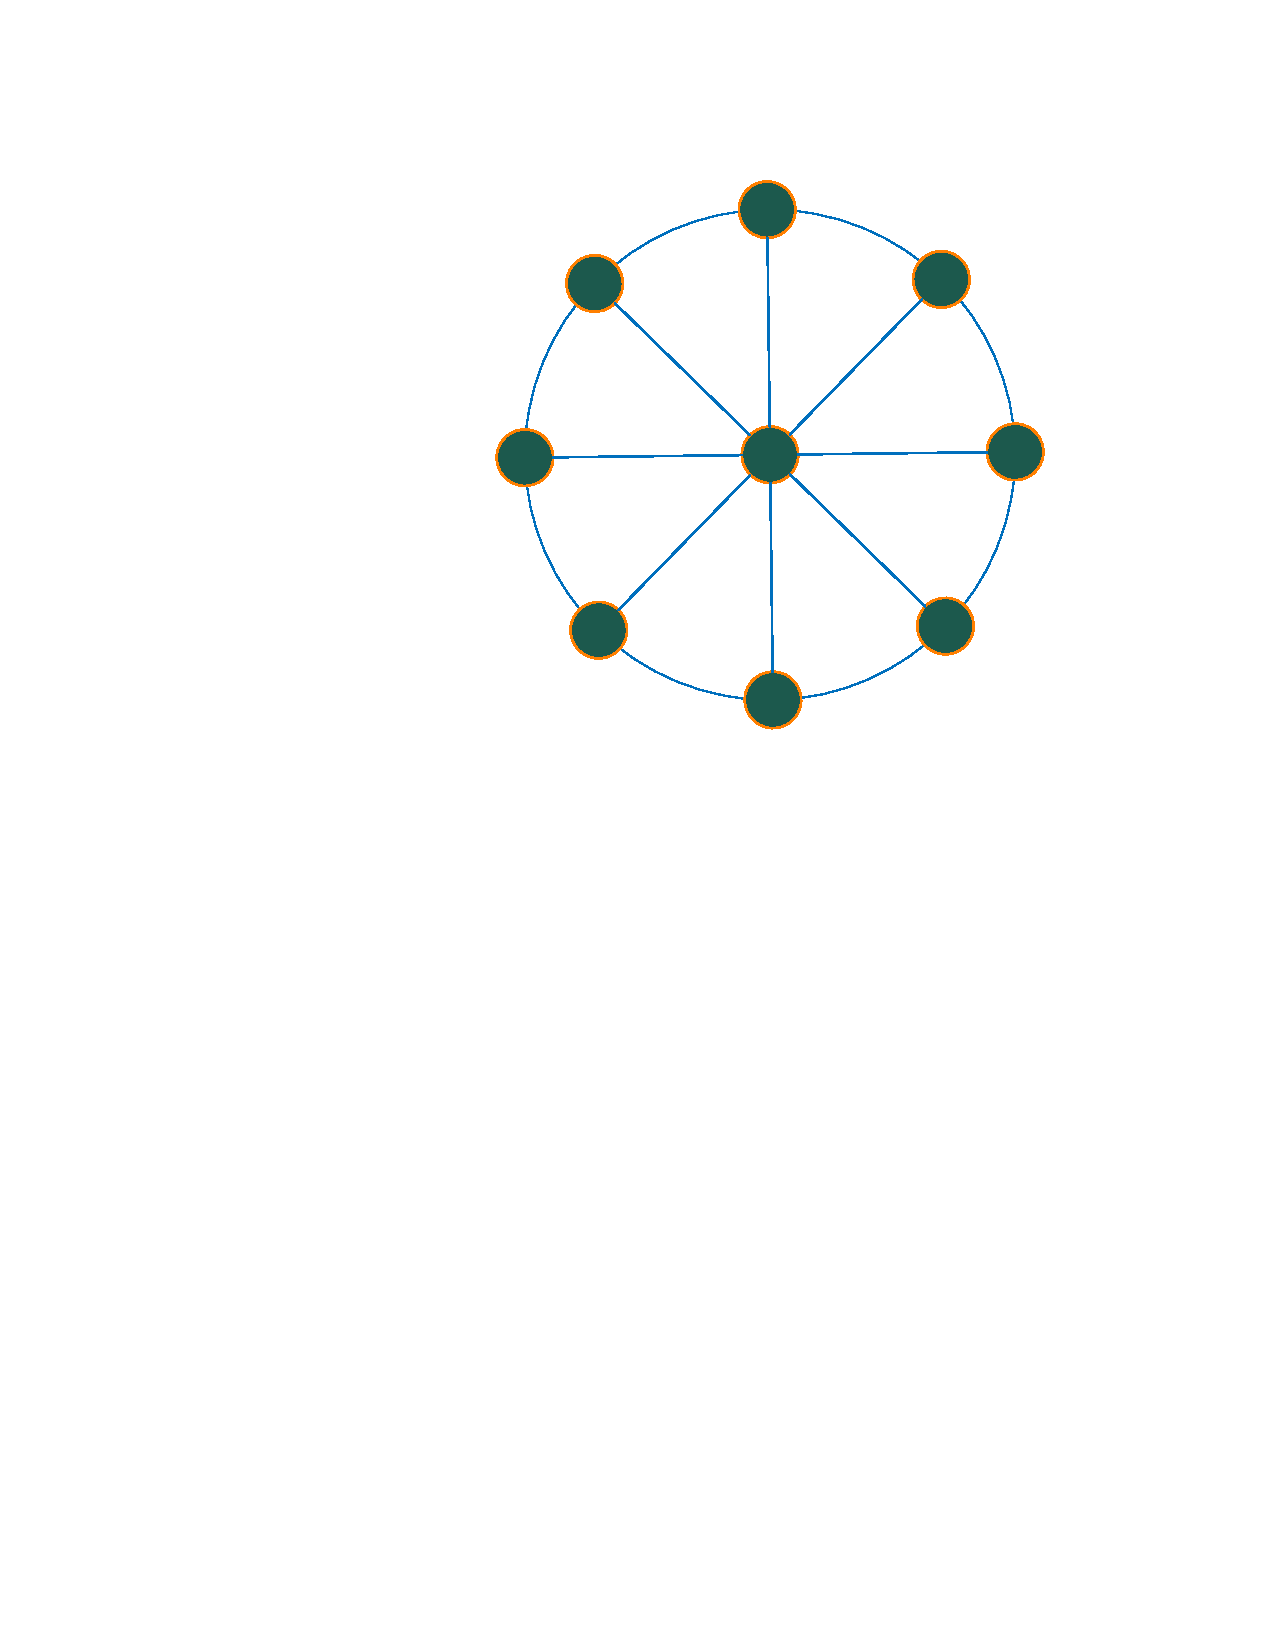
\includegraphics[width=0.65\linewidth]{P634}
		\vspace*{-10pt}
	\end{figure}
	\textbf{\color{thachthuctoanhoc}Lời giải} (\textit{dựa theo tất cả lời giải Tạp chí đã nhận được từ bạn đọc})\textbf{\color{thachthuctoanhoc}.}
	\vskip 0.05cm
	Giả sử Pi thực hiện được ý muốn của mình.
	\vskip 0.05cm
	Xét một cách điền bất kì của Pi, thỏa mãn các điều kiện $i)$ và $ii)$.
	\vskip 0.05cm
	Gọi $S$ là tổng của tám số ở tám hình tròn nhỏ, nằm trên đường tròn lớn. Theo $i)$, \linebreak $S = 66$.       \hfill              ($1$)
	\vskip 0.05cm
	Gọi $s$ là tổng của ba số ở ba hình tròn nhỏ, nằm trên cùng một đường kính tùy ý của đường tròn lớn. Do các số ở các hình tròn nhỏ là các số nguyên, nên $s$ là một số nguyên.
	\vskip 0.05cm
	Theo $ii)$, tổng của ba số ở ba hình tròn nhỏ, nằm trên mỗi đường kính, trong số ba đường kính còn lại của đường tròn lớn, cũng bằng $s$. Vì thế, từ quan sát hình đã cho ở đề bài, ta có:
	\begin{align*}
		4s = 4 \cdot 4 + S. \tag{$2$}
	\end{align*}
	Từ ($1$) và ($2$), suy ra $4s = 82$. Từ đây, vì $s$ là số nguyên nên $82$ chia hết cho $4$, là điều vô lý.
	\vskip 0.05cm
	Điều vô lý nhận được ở trên cho thấy, giả sử ở đầu lời giải là sai; nghĩa là, Pi \textit{không thể} thực hiện được ý muốn của mình.
	\vskip 0.05cm
	\textbf{\color{thachthuctoanhoc}Bình luận và Nhận xét}
	\vskip 0.05cm
	Tất cả lời giải Tạp chí đã nhận được từ bạn đọc đều là lời giải đúng và hoàn chỉnh.
	\vskip 0.15cm
	\hfill	\textbf{\color{thachthuctoanhoc}Nguyễn Khắc Minh}
	\vskip 0.15cm
	{\color{thachthuctoanhoc}{\usefont{T5}{qag}{b}{n} P635.}}
	(Mức $B$) Chứng minh rằng, với mọi số nguyên $n\ge2$, ta luôn có:
	\begin{align*}
		\dfrac{1}{2!}+\dfrac{2}{3!}+\ldots+\dfrac{2^{n-2}}{n!}\le\dfrac{3}{2}.
	\end{align*}
	(Với mỗi số nguyên dương $k$, $k!$ (đọc là, ``$k$ giai thừa") ký hiệu tích của $k$ số nguyên dương đầu tiên; tức là, $k!=1\cdot2\cdots k$.)
	\vskip 0.05cm
	\textbf{\color{thachthuctoanhoc}Lời giải} (\textit{phỏng theo ý giải của bạn Nguyễn Công Minh Đức, lớp $11$ Toán $1$, trường THPT chuyên Hưng Yên, tỉnh Hưng Yên})\textbf{\color{thachthuctoanhoc}.}
	\vskip 0.05cm
	Trước hết, ta chứng minh Nhận xét sau:
	\vskip 0.05cm
	\textbf{\color{thachthuctoanhoc}Nhận xét.} Với mọi số nguyên $k \ge 3$, ta có:
	\begin{align*}
		\frac{{{2^{k - 2}}}}{{k!}} \le 2\left( {\frac{1}{{k - 1}} - \frac{1}{k}} \right).
	\end{align*}
	\textit{Chứng minh.} Dễ thấy, bất đẳng thức cần chứng minh tương đương với bất đẳng thức
	\begin{align*}
		{2^{k - 3}} \le \left( {k - 2} \right)!. \tag{$*$}
	\end{align*}
	Với $k = 3$, hiển nhiên ($*$) là một bất đẳng thức đúng.
	\vskip 0.05cm
	Xét $k \ge 4$. Khi đó, $k - 2 \ge 2$. Do đó
	\begin{align*}
		\left( {k - 2} \right)! &= \left( {k - 2} \right)\left( {k - 3} \right) \cdots 2 \\
		&\ge \underbrace {2 \cdot 2 \cdot  \cdots  \cdot 2}_{k - 3\text{ thừa số }2} = {2^{k - 3}}.
	\end{align*}
	Bất đẳng thức ($*$) được chứng minh, và do đó, bất đẳng thức của Nhận xét được chứng minh.
	\vskip 0.05cm
	\textit{Trở lại bài toán.}
	\vskip 0.05cm
	Dễ thấy, với $n = 2$, bất đẳng thức của đề bài là một bất đẳng thức đúng.
	\vskip 0.05cm
	Xét $n \ge 3$. Khi đó, theo Nhận xét trên, ta có:
	\begin{align*}
			&\frac{1}{{2!}} + \frac{2}{{3!}} + \frac{{{2^2}}}{{4!}} +  \cdots  + \frac{{{2^{n - 2}}}}{{n!}} \\[-0.6ex]
			\le &\frac{1}{2} + 2\left( \left( {\frac{1}{2} - \frac{1}{3}} \right) + \left( {\frac{1}{3} - \frac{1}{4}} \right) +  \cdots \right. \\[-0.6ex]
				&\left.+ \left( {\frac{1}{{n - 1}} - \frac{1}{n}} \right) \right)\\[-0.6ex]
			 = &\frac{1}{2} + 2\left( {\frac{1}{2} - \frac{1}{n}} \right) = \frac{3}{2} - \frac{2}{n} < \frac{3}{2}.
	\end{align*}
	Vì vậy, bất đẳng thức của đề bài được chứng minh.
	\vskip 0.05cm
	\textbf{\color{thachthuctoanhoc}Bình luận và Nhận xét}
	\vskip 0.05cm
	Trong số các lời giải Tạp chí đã nhận được từ bạn đọc, rất tiếc, có hai lời giải không được chấp nhận là lời giải hoàn chỉnh, do người giải bài không chứng minh các đánh giá mang tính ``chìa khóa" trong lời giải.
	\vskip 0.05cm
	\hfill	\textbf{\color{thachthuctoanhoc}Lê Huy}
	\vskip 0.05cm
	{\color{thachthuctoanhoc}{\usefont{T5}{qag}{b}{n} P636.}}
	(Mức $B$) Cho tam giác nhọn $ABC$, nội tiếp đường tròn $(O)$. Xét lục giác lồi $MNPQRS$ có các đỉnh $M, N$ thuộc cạnh $BC$, các đỉnh $P, Q$ thuộc cạnh $CA$, các đỉnh $R, S$ thuộc cạnh $AB$, sao cho
	\begin{align*}
		\angle{ROQ} &=\angle{BAC},\; \angle{MOS} =\angle{CBA}\\[-0.6ex]
		&\text{\color{black}và}\;\angle{NOP}= \angle{ACB}.
	\end{align*}
	Chứng minh rằng 
	\begin{align*}
		MN + PQ + RS \leq NP + QR + SM.
	\end{align*}
	\textbf{\color{thachthuctoanhoc}Lời giải} (\textit{của bạn Trần Minh Hoàng, lớp $10$T$1$, trường THPT chuyên Hà Tĩnh, tỉnh Hà Tĩnh})\textbf{\color{thachthuctoanhoc}.}
	\begin{figure}[H]
		\centering
		\vspace*{-15pt}
		\captionsetup{labelformat= empty, justification=centering}
		\definecolor{qqwuqq}{rgb}{0.,0.39215686274509803,0.}
		\definecolor{uuuuuu}{rgb}{0.26666666666666666,0.26666666666666666,0.26666666666666666}
		\definecolor{ffqqqq}{rgb}{1.,0.,0.}
		\definecolor{xdxdff}{rgb}{0.49019607843137253,0.49019607843137253,1.}
		\definecolor{qqqqff}{rgb}{0.,0.,1.}
		\begin{tikzpicture}[scale=0.55,node font= \small]
			\draw [shift={(2.1249983220271007,1.0078498119199826)},,pattern color=qqwuqq,fill=qqwuqq,fill opacity=0.10000000149011612] (0,0) -- (-0.22029171081020696:0.4) arc (-0.22029171081020696:59.198829064869955:0.4) -- cycle;
			\draw [shift={(6.,2.)},,pattern color=qqwuqq,fill=qqwuqq,fill opacity=0.10000000149011612] (0,0) -- (169.1110677998218:0.4) arc (169.1110677998218:228.530188575502:0.4) -- cycle;
			\draw [shift={(6.,2.)},,pattern color=qqwuqq,fill=qqwuqq,fill opacity=0.10000000149011612] (0,0) -- (169.1110677998218:0.8) arc (169.1110677998218:194.3614146618134:0.8) -- cycle;
			\draw [shift={(6.,2.)},,pattern color=qqwuqq,fill=qqwuqq,fill opacity=0.10000000149011612] (0,0) -- (143.8607209378302:0.6) arc (143.8607209378302:169.1110677998218:0.6) -- cycle;
			\draw [shift={(6.,2.)},,pattern color=qqwuqq,fill=qqwuqq,fill opacity=0.10000000149011612] (0,0) -- (-165.63858533818663:0.8) arc (-165.63858533818663:-131.46981142449806:0.8) -- cycle;
			\draw [shift={(6.,2.)},,pattern color=qqwuqq,fill=qqwuqq,fill opacity=0.10000000149011612] (0,0) -- (-131.46981142449806:0.6) arc (-131.46981142449806:-97.30103751080952:0.6) -- cycle;
			\draw [shift={(6.,2.)},,pattern color=qqwuqq,fill=qqwuqq,fill opacity=0.10000000149011612] (0,0) -- (-14.801998083433794:0.6) arc (-14.801998083433794:104.0362434679265:0.6) -- cycle;
			\draw [] (6.,2.) circle (4.cm);
			\draw [,color=ffqqqq] (5.029857499854668,5.8805700005813275)-- (9.86725791928902,0.9780821042293271);
			\draw [] (5.029857499854668,5.8805700005813275)-- (2.769656915559922,4.359000541926636);
			\draw [,color=ffqqqq] (2.7696569155599233,4.359000541926637)-- (5.4916697208604015,-1.9675685661762485);
			\draw [] (2.1249983220271007,1.0078498119199826)-- (2.769656915559922,4.359000541926636);
			\draw [] (2.1249983220271007,1.0078498119199826)-- (5.4916697208604015,-1.9675685661762485);
			\draw (4.82,6.7) node[anchor=north west] {$A$};
			\draw (1.5,1.3) node[anchor=north west] {$B$};
			\draw (9.96,1.34) node[anchor=north west] {$C$};
			\draw [,color=qqqqff] (2.769656915559922,4.359000541926636)-- (3.054282279087836,2.566665720495411);
			\draw [,color=qqqqff] (2.9953665458938055,3.5115152528700584) -- (2.817594113369974,3.483284733311256);
			\draw [,color=qqqqff] (3.006345081277784,3.442381529110791) -- (2.8285726487539526,3.414151009551988);
			\draw [,color=qqqqff] (3.054282279087836,2.566665720495411)-- (5.112997902173607,0.9963614477074136);
			\draw [,color=qqqqff] (5.112997902173607,0.9963614477074136)-- (5.4916697208604015,-1.9675685661762485);
			\draw [,color=qqqqff] (5.382737068533431,-0.4047622562937149) -- (5.20418836232428,-0.4275736462346676);
			\draw [,color=qqqqff] (5.391608164621579,-0.4741978642639403) -- (5.213059458412428,-0.497009254204893);
			\draw [,color=qqqqff] (5.4004792607097265,-0.5436334722341657) -- (5.221930554500576,-0.5664448621751185);
			\draw [] (4.020312072968017,4.187120479685714)-- (7.151414984062024,3.730466848905957);
			\draw [] (7.320568549934373,0.9878737036679017)-- (8.521733569981919,2.341710554382787);
			\draw [] (6.,2.)-- (5.112997902173607,0.9963614477074136);
			\draw [] (6.,2.)-- (7.320568549934373,0.9878737036679017);
			\draw [] (6.,2.)-- (8.521733569981919,2.341710554382787);
			\draw [] (6.,2.)-- (7.151414984062024,3.730466848905957);
			\draw [] (6.,2.)-- (3.054282279087836,2.566665720495411);
			\draw [] (6.,2.)-- (2.1249983220271007,1.0078498119199826);
			\draw [] (6.,2.)-- (5.4916697208604015,-1.9675685661762485);
			\draw [] (6.,2.)-- (2.769656915559922,4.359000541926636);
			\draw [] (6.,2.)-- (4.020312072968017,4.187120479685714);
			\draw [] (6.,2.)-- (5.029857499854668,5.8805700005813275);
			\draw [] (6.,2.)-- (9.86725791928902,0.9780821042293271);
			\draw (4.3,1.) node[anchor=north west] {$M$};
			\draw (7.06,1.0) node[anchor=north west] {$N$};
			\draw (8.52,3.02) node[anchor=north west] {$P$};
			\draw (7.16,4.36) node[anchor=north west] {$Q$};
			\draw (3.52,4.94) node[anchor=north west] {$R$};
			\draw (2.44,3.14) node[anchor=north west] {$S$};
			\draw (5.75,1.9) node[anchor=north west] {$O$};
			\draw (2.3,5.06) node[anchor=north west] {$Y$};
			\draw (5.1,-1.95) node[anchor=north west] {$X$};
			\draw [,color=qqqqff] (3.054282279087836,2.566665720495411)-- (2.1249983220271007,1.0078498119199826);
			\draw [,color=qqqqff] (2.6848678641309616,1.7712355586239625) -- (2.5302569663172276,1.863406434052327);
			\draw [,color=qqqqff] (2.6490236347977087,1.711109098363066) -- (2.494412736983975,1.8032799737914305);
			\draw [] (3.054282279087836,2.566665720495411)-- (4.020312072968017,4.187120479685714);
			\draw [] (4.020312072968017,4.187120479685714)-- (5.029857499854668,5.8805700005813275);
			\draw [,color=qqqqff] (2.1249983220271007,1.0078498119199826)-- (5.112997902173607,0.9963614477074136);
			\draw [,color=qqqqff] (3.5493446620485978,1.0923741010308827) -- (3.5486525969333607,0.9123754314639203);
			\draw [,color=qqqqff] (3.619344144657972,1.0921049645971792) -- (3.618652079542735,0.912106295030217);
			\draw [,color=qqqqff] (3.6893436272673457,1.091835828163476) -- (3.6886515621521085,0.9118371585965136);
			\draw [] (5.112997902173607,0.9963614477074136)-- (7.320568549934373,0.9878737036679017);
			\draw [] (7.320568549934373,0.9878737036679017)-- (9.86725791928902,0.9780821042293271);
			\draw [shift={(6.,2.)},,color=qqwuqq] (169.1110677998218:0.8) arc (169.1110677998218:194.3614146618134:0.8);
			\draw[,color=qqwuqq] (5.2603397373977145,1.97757911850266) -- (5.140394829948694,1.9739432998814699);
			\draw [shift={(6.,2.)},,color=qqwuqq] (143.8607209378302:0.6) arc (143.8607209378302:169.1110677998218:0.6);
			\draw[,color=qqwuqq] (5.504840585513648,2.2154464068986366) -- (5.394805160072236,2.2633233862094446);
			\draw [shift={(6.,2.)},,color=qqwuqq] (-165.63858533818663:0.8) arc (-165.63858533818663:-131.46981142449806:0.8);
			\draw[,color=qqwuqq] (5.392811956659965,1.5770074704857064) -- (5.294349030712932,1.5084140873212266);
			\draw[,color=qqwuqq] (5.346794244564377,1.6522612459535508) -- (5.240868986926167,1.595871177729802);
			\draw [shift={(6.,2.)},,color=qqwuqq] (-131.46981142449806:0.6) arc (-131.46981142449806:-97.30103751080952:0.6);
			\draw[,color=qqwuqq] (5.806758084005368,1.4957604122019723) -- (5.7638154360065625,1.383707170469077);
			\draw[,color=qqwuqq] (5.748132023868733,1.522336391799061) -- (5.69216136250623,1.416188923309963);
			\draw [shift={(6.,2.)},,color=qqwuqq] (-14.801998083433794:0.6) arc (-14.801998083433794:104.0362434679265:0.6);
			\draw [shift={(6.,2.)},,color=qqwuqq] (-14.801998083433794:0.5) arc (-14.801998083433794:104.0362434679265:0.5);
			\draw [fill=qqqqff] (6.,2.) circle (1.5pt);
			\draw [fill=xdxdff] (5.029857499854668,5.8805700005813275) circle (1.5pt);
			\draw [fill=xdxdff] (9.86725791928902,0.9780821042293271) circle (1.5pt);
			\draw [fill=xdxdff] (2.769656915559922,4.359000541926636) circle (1.5pt);
			\draw [fill=xdxdff] (2.7696569155599233,4.359000541926637) circle (1.5pt);
			\draw [fill=xdxdff] (5.4916697208604015,-1.9675685661762485) circle (1.5pt);
			\draw [fill=xdxdff] (2.1249983220271007,1.0078498119199826) circle (1.5pt);
			\draw [fill=uuuuuu] (5.112997902173607,0.9963614477074136) circle (1.5pt);
			\draw [fill=uuuuuu] (3.054282279087836,2.566665720495411) circle (1.5pt);
			\draw [fill=xdxdff] (4.020312072968017,4.187120479685714) circle (1.5pt);
			\draw [fill=xdxdff] (7.151414984062024,3.730466848905957) circle (1.5pt);
			\draw [fill=xdxdff] (8.521733569981919,2.341710554382787) circle (1.5pt);
			\draw [fill=xdxdff] (7.320568549934373,0.9878737036679017) circle (1.5pt);
		\end{tikzpicture}
		\vspace*{-5pt}
	\end{figure}
	Gọi $X$ và $Y$, tương ứng, là điểm đối xứng với $B$ qua $OM$ và qua $OS$; ta có:
	\begin{align*}
		&OX = OB = OY; \tag{$1$}\\[-0.6ex]
		\text{và } &BM = XM, SB = SY. \tag{$2$}
	\end{align*}
	Từ ($1$) suy ra, $X, Y \in (O)$.
	\vskip 0.05cm
	Tiếp theo, ta có:
	\begin{align*}
		\angle XOY &= \angle XOB + \angle BOY \\[-0.6ex]
		&= 2\angle MOB + 2\angle BOS \\[-0.6ex]
		&= 2\angle MOS = 2\angle CBA = \angle COA.
	\end{align*}
	Mà $X, Y, A, C \in (O)$, nên $XY = CA$. \hfill ($3$)
	\vskip 0.05cm
  	Từ ($2$) suy ra
    \begin{align*}
    		BM + MS + SB &= XM + MS + SY \\[-0.6ex]
    		&\ge XS + SY \ge XY \\[-0.6ex]
    		&= CA \text{ (theo ($3$))}. \tag{$4$}  
    \end{align*}
    Bằng cách hoàn toàn tương tự, ta cũng chứng minh được:
	\begin{align*}
		&CP + PN + NC \ge AB,   \tag{$5$}\\[-0.6ex]
		&AR + RQ + QA \ge BC.  \tag{$6$}
	\end{align*}                      
	Cộng các bất đẳng thức ($4$), ($5$), ($6$), vế theo vế, ta được:
	\begin{align*}
		&(BM + MS + SB) + (CP + PN + NC) \\[-0.6ex]
		&+ (AR + RQ + QA) \ge CA + AB + BC.	
	\end{align*}
	Do đó
	\begin{align*}
		&NP + QR + SM\\[-0.6ex]
		 \ge &(BC - BM - NC) + (CA - CP - QA) \\[-0.6ex]
		 &+ (AB - AR - SB)\\[-0.6ex]
		  = \,&MN + PQ + RS.
	\end{align*}
	Ta có điều phải chứng minh theo yêu cầu đề bài.
	\vskip 0.05cm
	\textbf{\color{thachthuctoanhoc}Bình luận và Nhận xét}
	\vskip 0.05cm
	$\pmb{1.}$ Lời giải của bạn \textit{Trần Minh Hoàng} là lời giải duy nhất Tạp chí nhận được từ bạn đọc.
	\vskip 0.05cm
	$\pmb{2.}$ Một câu hỏi rất tự nhiên được đặt ra: \textit{Dấu đẳng thức ở bất đẳng thức của đề bài có thể xảy ra hay không?} Mời các bạn đọc có quan tâm cùng tìm hiểu.
	\vskip 0.05cm
	\hfill	\textbf{\color{thachthuctoanhoc}Hạ Vũ Anh}
	\vskip 0.05cm
	{\color{thachthuctoanhoc}{\usefont{T5}{qag}{b}{n} P637.}}
	(Mức $A$) Cho số thực $a\in(0;1)$. Cho dãy số $(x_n)$, xác định bởi: $x_1=a$  và 
	\columnbreak
	\begin{align*}
		x_{n+1}=x_n\left(1-\dfrac{x_n^3+x_n^4}2\right)\quad\text{\color{black}với mọi } n\ge 1.
	\end{align*}
	Chứng minh rằng, tồn tại vô số số nguyên dương $m$ sao cho 
	\begin{align*}
		\dfrac1{x_{m+1}}-\dfrac1{x_m}>\dfrac1{3\sqrt[3]{m^2}}.
	\end{align*}
	\textbf{\color{thachthuctoanhoc}Lời giải} (\textit{của người chấm bài})\textbf{\color{thachthuctoanhoc}.}
	\vskip 0.05cm
	Bằng phương pháp quy nạp theo $n \in \mathbb{N^*}$  dễ dàng chứng minh được rằng $x_n \in (0;1)$  với mọi $n\in\mathbb{N^*}$.  Vì thế, từ hệ thức xác định dãy $(x_n)$,  suy ra $x_{n+1} < x_n$  với mọi $n \in \mathbb{N^*}$.  Như vậy, $(x_n)$  là một dãy số giảm, bị chặn dưới bởi $0$; do đó, nó có giới hạn hữu hạn không âm, khi  $n \to + \infty$.
	\vskip 0.05cm
	Đặt $L = \lim {x_n}$.  Khi đó, chuyển hệ thức xác định dãy $(x_n)$  qua giới hạn, ta được:
	\begin{align*}
		L = L\left( {1 - \frac{{{L^3} + {L^4}}}{2}} \right);
	\end{align*}
	suy ra, $L = 0$ (do $L \ge 0$).
	\vskip 0.05cm
	Vì thế, đặt  ${y_n} = \frac{{x_n^3 + x_n^4}}{2}$, ta có  $\lim {y_n} = 0$ và  $\lim \frac{{{y_n}}}{{x_n^3}} = \frac{1}{2}$. \hfill ($1$)
	\vskip 0.05cm
	Từ hệ thức xác định dãy $(x_n)$  suy ra
	\begin{align*}
		\frac{1}{{x_{n \!+\! 1}^3}} \!-\! \frac{1}{{x_n^3}} &= \frac{1}{{x_n^3}}\left( {\frac{1}{{{{\left( {1 - {y_n}} \right)}^3}}} - 1} \right) \\[-0.6ex]
		&= \!\frac{{{y_n}}}{{x_n^3}} \!\cdot\! \frac{{3 \!-\! 3{y_n} \!+\! y_n^2}}{{{{\left( {1 \!-\! {y_n}} \right)}^3}}} \text{  với mọi } n \in \mathbb{N^*}
	\end{align*}
	Vì thế, do ($1$) nên
	\begin{align*}
		\lim \left( {\frac{1}{{x_{n + 1}^3}} - \frac{1}{{x_n^3}}} \right) = \frac{3}{2}.
	\end{align*}
	Do đó, theo định lý trung bình Cesaro, ta có $\lim \frac{1}{{nx_n^3}} = \frac{3}{2}$; suy ra,   $\lim nx_n^3 = \frac{2}{3}$. \hfill                                   ($2$)
	\vskip 0.05cm
	Tiếp theo, từ hệ thức xác định dãy $(x_n)$  ta có:
	\begin{align*}
		&\left( {\frac{1}{{{x_{n + 1}}}} - \frac{1}{{{x_n}}}} \right)\sqrt[3]{{{n^2}}}\\[-0.6ex]
		 = &\frac{1}{{{x_n}}} \cdot \left( {\frac{1}{{1 - {y_n}}} - 1} \right) \cdot \sqrt[3]{{{n^2}}} \\[-0.6ex]
		 = &\frac{1}{{{x_n}}} \cdot \frac{{{y_n}}}{{1 - {y_n}}} \cdot \sqrt[3]{{{n^2}}} \\[-0.6ex]
		 = &\frac{1}{{1 - {y_n}}} \cdot \frac{{{y_n}}}{{x_n^3}} \cdot {\left( {nx_n^3} \right)^{\frac{2}{3}}} \text{ với mọi } n\in \mathbb{N^*}.
	\end{align*}  
	Vì thế, từ ($1$) và ($2$), suy ra
	\begin{align*}
		\lim \left( {\left( {\frac{1}{{{x_{n + 1}}}} - \frac{1}{{{x_n}}}} \right)\sqrt[3]{{{n^2}}}} \right) = \frac{1}{2} \cdot {\left( {\frac{2}{3}} \right)^{\frac{2}{3}}}.
	\end{align*}
	Mà  $\frac{1}{3} < \frac{1}{2} \cdot {\left( {\frac{2}{3}} \right)^{\frac{2}{3}}}$, nên theo định nghĩa giới hạn hữu hạn, tồn tại số nguyên dương  $n_0$, sao cho với mọi $n \ge n_0$  ta có
	\begin{align*}
		\left( {\frac{1}{{{x_{n + 1}}}} - \frac{1}{{{x_n}}}} \right)\sqrt[3]{{{n^2}}} > \frac{1}{3}.
	\end{align*}
	Do đó, có vô số số nguyên dương $m$, sao cho
	\begin{align*}
		\frac{1}{{{x_{m + 1}}}} - \frac{1}{{{x_m}}} > \frac{1}{{3\sqrt[3]{{{m^2}}}}}.
	\end{align*}
	Ta có điều phải chứng minh theo yêu cầu đề bài.
	\vskip 0.05cm
	\textbf{\color{thachthuctoanhoc}Bình luận và Nhận xét}
	\vskip 0.05cm
	$\pmb{1.}$ Bài đã ra là một bài tập khá cơ bản, thuộc chủ đề ``Ứng dụng của định lí trung bình Cesaro trong việc nghiên cứu tiệm cận của các dãy số, được cho bởi hệ thức truy hồi dạng ${x_{n + 1}} = {x_n} + a \cdot x_n^\alpha .$". Việc có thêm số hạng $-\dfrac{1}{2}x_n^5$ trong hệ thức truy hồi của dãy $(x_n)$  ở đề bài chỉ gây thêm chút rắc rối về kĩ thuật. Trong lời giải trên, rắc rối này đã được xử lý bằng phép đặt  ${y_n} = \frac{{x_n^3 + x_n^4}}{2}$.
	\vskip 0.05cm
	$\pmb{2.}$ Với việc hiểu định nghĩa giới hạn hữu hạn của một dãy số, ở mức tối thiểu cần thiết, dễ thấy, điều phải chứng minh theo yêu cầu của bài toán có thể rút ra được từ việc khảo sát tính hội tụ của dãy $(u_n)$  xác định bởi
	\begin{align*}
		{u_n} = \left( {\frac{1}{{{x_{n + 1}}}} - \frac{1}{{{x_n}}}} \right)\sqrt[3]{{{n^2}}} \text{ với mọi } n \in \mathbb{N^*}
	\end{align*}
	Nhận xét nêu trên là một ``chìa khóa", giúp xác định hướng giải bài đã ra.
	\vskip 0.05cm
	$\pmb{3.}$ Tới thời điểm bản thảo vào Nhà in, Tạp chí mới chỉ nhận được đúng một lời giải từ bạn đọc. Đó là, lời giải của bạn \textit{Trần Minh Hoàng} (lớp $10$T$1$, trường THPT chuyên Hà Tĩnh, tỉnh Hà Tĩnh). Ý tưởng giải của bạn Trần Minh Hoàng, về cơ bản, giống ý tưởng của lời giải trên đây; điểm khác biệt nằm ở kĩ thuật xử lí. Bạn Hoàng đã xử lý bằng cách chuyển dãy $(x_n)$  về dãy  $\left(\dfrac{1}{x_n}\right)$, rồi khảo sát tính hội tụ của dãy này. Lời giải của bạn Hoàng là một lời giải đúng và hoàn chỉnh.
	\vskip 0.05cm
	\hfill	\textbf{\color{thachthuctoanhoc}Trần Nam Dũng}
	\vskip 0.05cm
	{\color{thachthuctoanhoc}{\usefont{T5}{qag}{b}{n} P638.}}
	(Mức $A$) Tìm hai chữ số tận cùng của số $T=22^{3^{2002}}+22^{4^{2003}}$.
	\vskip 0.05cm
	\textbf{\color{thachthuctoanhoc}Lời giải} (\textit{dựa theo cách giải của bạn Võ Trần Hiền, lớp $12$ Toán $1$, trường THPT chuyên Tiền Giang, tỉnh Tiền Giang})\textbf{\color{thachthuctoanhoc}.}
	\vskip 0.05cm
	Trước hết, dễ thấy, $T \equiv 0\left( {\bmod 4} \right)$. \hfill ($1$)
	\vskip 0.05cm
	Tiếp theo, do  $22 \equiv  - 3\left( {\bmod 25} \right)$ nên
	\begin{align*}
		T &\equiv {\left( { - 3} \right)^{{3^{2002}}}} + {\left( { - 3} \right)^{{4^{2003}}}} \\
		&\equiv  - {3^{{3^{2002}}}} + {3^{{4^{2003}}}}\left( {\bmod 25} \right). \tag{$2$}
	\end{align*}
	Do  ${3^3} \equiv 2\left( {\bmod 25} \right)$ nên
	\begin{align*}
		{3^{20}} &= {\left( {{3^3}} \right)^6} \cdot {3^2} \equiv {2^6} \cdot 9 \equiv 14 \cdot 9 \\
		&\equiv 1\left( {\bmod 25} \right). \tag{$3$}
	\end{align*}
	Vì
	\begin{align*}
		{3^{2002}} &\equiv {\left( { - 1} \right)^{2002}} = 1 \equiv 9\left( {\bmod 4} \right),\\
		{3^{2002}} &= {\left( {{3^2}} \right)^{1001}} \equiv {\left( { - 1} \right)^{1001}} =  - 1 \\
		&\equiv 9\left( {\bmod 5} \right),
	\end{align*}
	và $(4, 5) = 1$, nên ${3^{2002}} \equiv 9\left( {\bmod 20} \right)$.  Do đó, tồn tại số nguyên dương $k$, sao cho
	\begin{align*}
		{3^{2002}} = 20k + 9.
	\end{align*}
	Vì thế, theo ($3$), ta có:
	\begin{align*}
		{3^{{4^{2003}}}} \!\!=\!\! {\left( {{3^{20}}} \right)^m} \!\!\cdot\! {3^4} \!\equiv\! 1 \!\!\cdot\! 6 \!=\! 6\left(\! {\bmod 25} \right)\!\!. \tag{$4$}
	\end{align*}
	Do
	\begin{align*}
		{4^{2003}} \equiv 0 \equiv 4\left( {\bmod 4} \right),\\
		{4^{2003}} \equiv {\left( { - 1} \right)^{2003}} =  - 1 \equiv 4\left( {\bmod 5} \right),
	\end{align*}
	và $(4, 5) = 1$, nên ${4^{2003}} \equiv 4\left( {\bmod 20} \right)$.  Do đó, tồn tại số nguyên dương $m$, sao cho
	\begin{align*}
		{4^{2003}} = 20m + 4.
	\end{align*}
	Vì thế, theo ($3$), ta có:
	\begin{align*}
		{3^{{4^{2003}}}} \!\!=\!\! {\left(\! {{3^{20}}} \right)^m} \!\!\cdot\! {3^4} \!\equiv \!\!1 \!\!\cdot\! 6 \!=\! 6\left(\! {\bmod 25} \right). \tag{$5$}
	\end{align*}
	Từ ($2$), ($4$), ($5$) suy ra
	\begin{align*}
		T \equiv  - 8 + 6 =  - 2 \equiv 48\left( {\bmod 25} \right). \tag{$6$}
	\end{align*}
	Từ ($1$) và ($6$), với lưu ý $0 \equiv 48\left( {\bmod 4} \right)$ và $(4, 25) = 1$, ta có  $T \equiv 48\left( {\bmod 100} \right)$.
	\vskip 0.05cm
	Vì vậy, hai chữ số tận cùng của số $T$ là $48$.
	\vskip 0.05cm
	\textbf{\color{thachthuctoanhoc}Bình luận và Nhận xét}
	\vskip 0.05cm
	$\pmb{1.}$ Có thể phát hiện ra ($3$) (trong Lời giải trên) nhờ Định lý Euler. Định lí được phát biểu như sau:
	\vskip 0.05cm
	\textbf{\color{thachthuctoanhoc}Định lý Euler.} \textit{Nếu số nguyên $a$ và số nguyên $m > 1$ nguyên tố cùng nhau thì  ${a^{\varphi \left( m \right)}} \equiv 1\left( {\bmod m} \right);$ trong đó, $\varphi \left( m \right)$  là giá trị của Phi -- hàm Euler tại $m$}.
	\vskip 0.05cm
	$\pmb{2.}$ Bài đã ra là một bài toán cơ bản, có dạng quen thuộc, thích hợp cho việc luyện tập của các bạn học sinh, khi học về chủ đề ``Đồng dư".
	\vskip 0.05cm
	$\pmb{3.}$ Trong số các lời giải Tạp chí đã nhận được từ bạn đọc, rất tiếc, có hai lời giải cho kết quả sai, tuy cách giải đúng, do người giải bài đã thực hiện sai một số tính toán.
	\begin{flushright}
		\textbf{\color{thachthuctoanhoc}Lưu Thị Thanh Hà}
	\end{flushright}
	{\color{thachthuctoanhoc}{\usefont{T5}{qag}{b}{n} P639.}}
	(Mức $A$) Cho tam giác nhọn, không cân $A B C$, nội tiếp đường tròn $(O)$. Tiếp tuyến tại $B$ và $C$ của đường tròn $(O)$ cắt nhau tại $P$. Gọi $M$ là điểm chính giữa của cung $B C$ không chứa $A$ của đường tròn $(O)$. Đoạn thẳng $A M$ cắt đường tròn tâm $P$, bán kính $P B$ tại điểm $S$. Gọi $E, F$ tương ứng là hình chiếu vuông góc của $S$ trên $A C, A B$; $T, D$ tương ứng là giao điểm của $B C$ với các đường thẳng $E F$, $SO$.  Chứng minh rằng $ST \perp A D$.
	\vskip 0.05cm
	\textbf{\color{thachthuctoanhoc}Lời giải} (\textit{dựa theo đa số lời giải Tạp chí đã nhận được từ bạn đọc})\textbf{\color{thachthuctoanhoc}.}
	\begin{figure}[H]
		\centering
		\vspace*{-10pt}
		\captionsetup{labelformat= empty, justification=centering}
		\definecolor{qqwuqq}{rgb}{0.,0.39215686274509803,0.}
		\definecolor{ffqqqq}{rgb}{1.,0.,0.}
		\definecolor{uuuuuu}{rgb}{0.26666666666666666,0.26666666666666666,0.26666666666666666}
		\definecolor{xdxdff}{rgb}{0.49019607843137253,0.49019607843137253,1.}
		\definecolor{qqqqff}{rgb}{0.,0.,1.}
		\hspace*{-5pt}\begin{tikzpicture}[scale=0.5,node font= \small]
			\draw[,pattern color=qqwuqq,fill=qqwuqq,fill opacity=0.10000000149011612] (1.0642825181395839,-0.32600353184726816) -- (1.3841048658990907,-0.3888701734502005) -- (1.446971507502023,-0.06904782569069373) -- (1.1271491597425163,-0.00618118408776137) -- cycle; 
			\draw[,pattern color=qqwuqq,fill=qqwuqq,fill opacity=0.10000000149011612] (4.72405089162533,0.7919487597595202) -- (4.936002901027053,0.544330314438081) -- (5.183621346348492,0.7562823238398035) -- (4.9716693369467695,1.0039007691612427) -- cycle; 
			\draw[,pattern color=qqwuqq,fill=qqwuqq,fill opacity=0.10000000149011612] (3.3646529416171456,0.5816846837515599) -- (3.2818280504023267,0.8969283770240626) -- (2.9665843571298236,0.8141034858092435) -- (3.049409248344643,0.49885979253674073) -- cycle; 
			\draw[,pattern color=qqwuqq,fill=qqwuqq,fill opacity=0.10000000149011612] (0.005609615150715119,2.5823675329086995) -- (0.22914039673662048,2.3451491979587455) -- (0.46635873168657477,2.5686799795446507) -- (0.2428279501006694,2.805898314494605) -- cycle; 
			\draw[,pattern color=ffqqqq,fill=ffqqqq,fill opacity=0.10000000149011612] (2.334126191639962,-0.5574586416074678) -- (2.3763303729707674,-0.8806572737689158) -- (2.699529005132215,-0.8384530924381102) -- (2.6573248238014098,-0.5152544602766622) -- cycle; 
			\draw [shift={(3.294006890231521,-0.4321147353279945)},,pattern color=qqwuqq,fill=qqwuqq,fill opacity=0.10000000149011612] (0,0) -- (168.87930187504327:0.4609523809523809) arc (168.87930187504327:202.65380426003037:0.4609523809523809) -- cycle;
			\draw [shift={(7.118830083440415,-1.5045755949116524)},,pattern color=qqwuqq,fill=qqwuqq,fill opacity=0.10000000149011612] (0,0) -- (130.5622729252014:0.4609523809523809) arc (130.5622729252014:164.33677531018847:0.4609523809523809) -- cycle;
			\draw [shift={(3.294006890231521,-0.4321147353279945)},,pattern color=qqwuqq,fill=qqwuqq,fill opacity=0.10000000149011612] (0,0) -- (-15.663224689811544:0.4609523809523809) arc (-15.663224689811544:40.56227292520137:0.4609523809523809) -- cycle;
			\draw [shift={(0.8422859120970068,-1.4553699800761124)},,pattern color=qqwuqq,fill=qqwuqq,fill opacity=0.10000000149011612] (0,0) -- (22.653804260030366:0.4609523809523809) arc (22.653804260030366:78.87930187504327:0.4609523809523809) -- cycle;
			\draw [] (4.,1.) circle (4.cm);
			\draw [] (2.0066093828095735,4.467909146344115)-- (0.8422859120970068,-1.4553699800761124);
			\draw [] (2.0066093828095735,4.467909146344115)-- (7.118830083440415,-1.5045755949116524);
			\draw [] (3.968642551385718,-2.9998770869135973)-- (2.0066093828095735,4.467909146344115);
			\draw [,color=ffqqqq] (2.782073531884239,-1.4705771450185317)-- (2.0066093828095735,4.467909146344115);
			\draw [] (2.782073531884239,-1.4705771450185317)-- (4.,1.);
			\draw [] (-4.2371135399578375,-1.4155495046344224)-- (4.9716693369467695,1.0039007691612427);
			\draw [] (4.9716693369467695,1.0039007691612427)-- (3.294006890231521,-0.4321147353279945);
			\draw [] (1.1271491597425163,-0.00618118408776137)-- (3.294006890231521,-0.4321147353279945);
			\draw [] (-4.2371135399578375,-1.4155495046344224)-- (2.0066093828095735,4.467909146344115);
			\draw [,color=ffqqqq] (-4.2371135399578375,-1.4155495046344224)-- (3.294006890231521,-0.4321147353279945);
			\draw [] (0.2428279501006694,2.805898314494605)-- (3.294006890231521,-0.4321147353279945);
			\draw [] (7.118830083440415,-1.5045755949116524)-- (-4.2371135399578375,-1.4155495046344224);
			\draw [] (0.8422859120970068,-1.4553699800761124)-- (3.9494244691519036,-5.4512872040761735);
			\draw [] (7.118830083440415,-1.5045755949116524)-- (3.9494244691519036,-5.4512872040761735);
			\draw [shift={(3.9494244691519036,-5.4512872040761735)},]  plot[domain=0.4749087318452353:2.680215050056665,variable=\t]({1.*5.061784712312204*cos(\t r)+0.*5.061784712312204*sin(\t r)},{0.*5.061784712312204*cos(\t r)+1.*5.061784712312204*sin(\t r)});
			\draw (1.6105714285714284,5.560380952380956) node[anchor=north west] {$A$};
			\draw (0.3914285714285726,-1.5312380952380986) node[anchor=north west] {$B$};
			\draw (7.238095238095237,-0.9546666666666698) node[anchor=north west] {$C$};
			\draw (2.5899047619047614,-1.3851428571428604) node[anchor=north west] {$D$};
			\draw (5.025523809523809,1.788) node[anchor=north west] {$E$};
			\draw (0.4525714285714286,0.82) node[anchor=north west] {$F$};
			\draw (3.711809523809523,1.903238095238095) node[anchor=north west] {$O$};
			\draw (3.665714285714285,-5.241523809523817) node[anchor=north west] {$P$};
			\draw (3.3333333333327,-3.193333333333383) node[anchor=north west] {$M$};
			\draw (-5.061904761904761,-0.9546666666666698) node[anchor=north west] {$T$};
			\draw (-0.331428571428569,3.608761904761906) node[anchor=north west] {$Y$};
			\draw (3.1430476190476184,-0.1940952380952404) node[anchor=north west] {$S$};
			\draw (1.8910476190476189,1.374285714285702) node[anchor=north west] {$X$};
			\draw (3.043428571428571,0.82) node[anchor=north west] {$I$};
			\draw [] (3.294006890231521,-0.4321147353279945)-- (7.118830083440415,-1.5045755949116524);
			\draw [] (3.294006890231521,-0.4321147353279945)-- (0.8422859120970068,-1.4553699800761124);
			\draw [shift={(3.294006890231521,-0.4321147353279945)},,color=qqwuqq] (-15.663224689811544:0.4609523809523809) arc (-15.663224689811544:40.56227292520137:0.4609523809523809);
			\draw [shift={(3.294006890231521,-0.4321147353279945)},,color=qqwuqq] (-15.663224689811544:0.34571428571428564) arc (-15.663224689811544:40.56227292520137:0.34571428571428564);
			\draw [shift={(0.8422859120970068,-1.4553699800761124)},,color=qqwuqq] (22.653804260030366:0.4609523809523809) arc (22.653804260030366:78.87930187504327:0.4609523809523809);
			\draw [shift={(0.8422859120970068,-1.4553699800761124)},,color=qqwuqq] (22.653804260030366:0.34571428571428564) arc (22.653804260030366:78.87930187504327:0.34571428571428564);
			\draw [] (2.2744532672679885,2.4167669523695663) circle (2.0685561743265515cm);
				\draw [fill=qqqqff] (4.,1.) circle (1.5pt);
				\draw [fill=xdxdff] (2.0066093828095735,4.467909146344115) circle (1.5pt);
				\draw [fill=xdxdff] (0.8422859120970068,-1.4553699800761124) circle (1.5pt);
				\draw [fill=xdxdff] (7.118830083440415,-1.5045755949116524) circle (1.5pt);
				\draw [fill=uuuuuu] (3.968642551385718,-2.9998770869135973) circle (1.5pt);
				\draw [fill=uuuuuu] (3.9494244691519036,-5.4512872040761735) circle (1.5pt);
				\draw [fill=uuuuuu] (3.294006890231521,-0.4321147353279945) circle (1.5pt);
				\draw [fill=uuuuuu] (1.1271491597425163,-0.00618118408776137) circle (1.5pt);
				\draw [fill=uuuuuu] (4.9716693369467695,1.0039007691612427) circle (1.5pt);
				\draw [fill=uuuuuu] (-4.2371135399578375,-1.4155495046344224) circle (1.5pt);
				\draw [fill=uuuuuu] (2.782073531884239,-1.4705771450185317) circle (1.5pt);
				\draw [fill=uuuuuu] (0.2428279501006694,2.805898314494605) circle (1.5pt);
				\draw [fill=uuuuuu] (2.542297151726403,0.36562475839501835) circle (1.5pt);
				\draw [fill=uuuuuu] (3.049409248344643,0.49885979253674073) circle (1.5pt);
		\end{tikzpicture}
		\vspace*{-15pt}
	\end{figure}
	Vì $S$ nằm trong góc nhọn $BAC$ nên từ các giả thiết $SE \bot AC$, $SF \bot AB$, suy ra $AFSE$ là tứ giác nội tiếp. Do đó
	\begin{align*}
		\angle FSE = {180^{\circ}} - \angle BAC. \tag{$1$}
	\end{align*}
	Do $PB$, $PC$ tiếp xúc với $(O)$, tương ứng, tại $B$, $C$ nên $PB = PC$. Do đó, $C \in (P; PB)$; suy ra
	\begin{align*}
		\angle BSC = &\frac{1}{2}\!\left({{{360}^{\circ}} \!-\! \angle BPC} \right) \!=\! {180^{\circ}} \!-\! \frac{1}{2}\angle BPC\\[-0.5ex]
		 = \,&{180^{\circ}} - \frac{1}{2}\left( {{{180}^{\circ}} - \angle BOC} \right)\\[-0.5ex]
		&\,\text{(do $PBOC$ là tứ giác nội tiếp)}\\[-0.5ex]
		= \,&{90^{\circ}} + \angle BAC. \tag{$2$}
	\end{align*}
	Từ ($1$) và ($2$), suy ra
	\begin{align*}
		\angle FSE + \angle BSC = {270^{\circ}};
	\end{align*}
	do đó
	\begin{align*}
		\angle BSF + \angle CSE = {90^{\circ}}.
	\end{align*}
	Suy ra,  $\angle BSF = \angle SCE$. Vì vậy, tam giác vuông (tại $F$) $BFS$ đồng dạng với tam giác vuông (tại $E$) $SEC$. Suy ra
	\begin{align*}
		\frac{{SB}}{{CS}} = \frac{{SF}}{{CE}} = \frac{{FB}}{{ES}}. \tag{$3$}
	\end{align*}
	Áp dụng định lý Menelaus cho tam giác ABC với cát tuyến EFT, ta được:
	\begin{align*}
		\frac{{TB}}{{TC}} \cdot \frac{{EC}}{{EA}} \cdot \frac{{FA}}{{FB}} = 1;
	\end{align*}
	suy ra
	\begin{align*}
		\frac{{TB}}{{TC}} = \frac{{EA}}{{EC}} \cdot \frac{{FB}}{{FA}}. \tag{$4$}
	\end{align*}
	Vì $M$ là điểm chính giữa của cung $BC$ không chứa $A$ của $(O)$, nên $AM$ là tia phân giác của góc $BAC$. Do đó, từ các giả thiết $S \in AM$ và $SE \bot AC$, $SF \bot AB$, suy ra
	\begin{align*}
		SE = SF \text{ và } EA = FA.  \tag{$5$}
	\end{align*} 
	Từ ($4$), ($5$) và ($3$), ta được:
	\begin{align*}
		\frac{{TB}}{{TC}} \!=\! \frac{{FA}}{{EC}} \!\cdot\! \frac{{FB}}{{FA}} \!=\! \frac{{FB}}{{EC}} \!=\! \frac{{FB}}{{ES}} \!\cdot\! \frac{{FS}}{{EC}} \!=\! {\left( {\frac{{SB}}{{SC}}} \right)^2}.
	\end{align*}
	Do đó, $ST$ là đường đối trung ngoài của tam giác $SBC$. \hfill ($6$)
	\vskip 0.05cm
	Do $P$ là tâm đường tròn $(SBC)$ và $OB \bot PB$, $OC \bot PC$, nên $OB$, $OC$ là các tiếp tuyến tại $B$, $C$ của ($SBC$). Vì thế, $SD$ là đường đối trung của tam giác $SBC$. \hfill ($7$)
	\vskip 0.05cm
	Từ ($6$) và ($7$), suy ra  $\left( {TDBC} \right) =  - 1.$            ($8$)
	\vskip 0.05cm
	Gọi $I$ là giao điểm của $AS$ và $EF$. Do ($5$) nên $AS$ là trung trực của $EF$; vì thế,  $AI \bot EF$, hay $AS \bot TI$, và $I$ là trung điểm của $EF$. \hfill ($9$)
	\vskip 0.05cm
	Gọi $X$ là giao điểm của $AD$ và $EF$.
	\vskip 0.05cm
	Do phép chiếu xuyên tâm bảo toàn tỷ số kép, nên từ ($8$) suy ra $\left( {TXFE} \right) =  - 1$.  Vì thế, do ($9$) nên theo hệ thức Maclaurin, ta có:
	\begin{align*}
		\overline {TX}  \cdot \overline {TI}  = \overline {TF}  \cdot \overline {TE}  = {P_{{T \mathord{\left/
						{\vphantom {T {\left( {AFSE} \right)}}} \right.
						\kern-\nulldelimiterspace} {\left( {AFSE} \right)}}}}.\tag{$10$}
	\end{align*}
	Gọi $Y$ là hình chiếu vuông góc của $S$ trên $TA$; ta có, $Y$ thuộc đường tròn $(AFSE)$. Do đó
	\begin{align*}
		\overline {TY}  \cdot \overline {TA}  = {P_{{T \mathord{\left/
						{\vphantom {T {\left( {AFSE} \right)}}} \right.
						\kern-\nulldelimiterspace} {\left( {AFSE} \right)}}}}. \tag{$11$}
	\end{align*}
	Từ ($10$) và ($11$), suy ra
	\begin{align*}
		\overline {TX}  \cdot \overline {TI}  = \overline {TY}  \cdot \overline {TA} .
	\end{align*}
	Do đó, $AYXI$ là tứ giác nội tiếp. Mà $\angle AIX = {90^{\circ}}$  (theo ($9$)), nên $\angle XYA = {90^{\circ}}$.  Suy ra, ba điểm $S$, $X$, $Y$ thẳng hàng. Do đó, từ định nghĩa điểm $Y$ và ($9$) suy ra, $X$ là trực tâm tam giác $ATS$. Vì vậy, $AX \bot ST$; mà $X \in AD$, nên $AD \bot ST$.
	\vskip 0.05cm
	Ta có điều phải chứng minh theo yêu cầu đề bài.
	\vskip 0.05cm
	\textbf{\color{thachthuctoanhoc}Bình luận và Nhận xét}
	\vskip 0.05cm
	Tất cả các lời giải Tạp chí đã nhận được từ bạn đọc đều là lời giải đúng và hoàn chỉnh.
	\vskip 0.05cm
	\hfill	\textbf{\color{thachthuctoanhoc}Hạ Vũ Anh}
	\vskip 0.05cm
	{\color{thachthuctoanhoc}{\usefont{T5}{qag}{b}{n} P640.}}
	(Mức $A$) Ký hiệu $S$ là tập hợp $2022$ số nguyên dương đầu tiên. Hỏi, có tất cả bao nhiêu tập con khác rỗng của $S$ mà tổng tất cả các số thuộc mỗi tập con đều chia hết cho $1024$?
	\vskip 0.05cm
	\textbf{\color{thachthuctoanhoc}Lời giải} (\textit{của người chấm bài})\textbf{\color{thachthuctoanhoc}.}
	\vskip 0.05cm
	$\bullet$ Xét bài toán khái quát sau của bài đã ra:
	\vskip 0.05cm
	\textbf{\color{thachthuctoanhoc}Bài toán khái quát.} \textit{Cho các số nguyên dương $k$, $n$, thỏa mãn $2^k < n$. Ký hiệu $S$ là tập hợp $n$ số nguyên dương đầu tiên. Hỏi, có tất cả bao nhiêu tập con khác rỗng của $S$, mà tổng tất cả các số thuộc mỗi tập con đều chia hết cho  $2^k$?}
	\vskip 0.05cm
	\textbf{\color{thachthuctoanhoc}Lời giải bài toán khái quát.}
	\vskip 0.05cm
	Ở lời giải này, ta quy ước:
	\vskip 0.05cm
	$1/$ Coi $0$ là tổng các số thuộc tập rỗng.
	\vskip 0.05cm
	$2/$ Coi phép chia hết cho $2^k$  là phép chia có số dư bằng  $2^k$.
	\vskip 0.05cm
	Ta biết rằng, mỗi số nguyên dương m đều được biểu diễn một cách duy nhất dưới dạng:
	\begin{align*}
		m &= {a_s} \cdot {2^s} + {a_{s - 1}} \cdot {2^{s - 1}} + {a_{s - 2}} \cdot {2^{s - 2}} +  \cdots  \\
		&+ {a_0} \cdot {2^0},
	\end{align*}
	trong đó, $s$ là một số tự nhiên, và  ${a_i} \in \left\{ {0;1} \right\}$ với mọi  $i = 0,1, \ldots ,s, $ ${a_s} \ne 0.$
	\vskip 0.05cm  
	Do đó, mỗi số nguyên dương  $m \le {2^k} - 1$ đều được biểu diễn một cách \textit{duy nhất} dưới dạng:
	\begin{align*}
		m = {a_{k - 1}} \cdot {2^{k - 1}} + {a_{k - 2}} \cdot {2^{k - 2}} +  \cdots  + {a_0} \cdot {2^0},
	\end{align*}
	trong đó, ${a_i} \in \left\{ {0;1} \right\}$  với mọi  $i = 0,1, \ldots,$ $k - 1$.
	\vskip 0.05cm
	Vì thế, với qui ước $1/$, ta có:
	\vskip 0.05cm
	\textbf{\color{thachthuctoanhoc}Nhận xét} $\pmb{1.}$ Với mỗi số tự nhiên $m \le {2^k} - 1,$  có \textit{đúng một} tập con của tập
	\begin{align*}
		{S_1} = \left\{ {{2^0},{2^1}, \ldots ,{2^{k - 1}}} \right\},
	\end{align*}
	mà tổng tất cả các số thuộc tập con đó bằng $m$.
	\vskip 0.05cm
	Ký hiệu ${S_2} = {S \mathord{\left/
			{\vphantom {S {{S_1}}}} \right.
			\kern-\nulldelimiterspace} {{S_1}}}$.  Ta có:
		\vskip 0.05cm
	\textbf{\color{thachthuctoanhoc}Nhận xét} $\pmb{2.}$ Mỗi tập con $X$ của $S$ đều biểu diễn được một cách duy nhất dưới dạng:
	\begin{align*}
		X = {X_1} \cup {X_2},
	\end{align*}
	trong đó, $X_1$  là một tập con của  $S_1$, và $X_2$  là một tập con của $S_2$.
	\vskip 0.05cm 
	Vì
	\begin{align*}
		{2^0} + {2^1} +  \cdots  + {2^{k - 1}} = {2^k} - 1
	\end{align*}
	nên tổng tất cả các số thuộc một tập con khác rỗng tùy ý của $S_1$  là một số nguyên dương không vượt quá $2^k -1$.  Do đó, với các qui ước $1/$ và $2/$, từ Nhận xét $2$ suy ra:
	\vskip 0.05cm
	\textbf{\color{thachthuctoanhoc}Nhận xét} $\pmb{3.}$ Tập con $T$ khác rỗng của $S$ có tính chất đề bài yêu cầu khi và chỉ khi nó có dạng:
	\begin{align*}
		T = {T_1} \cup {T_2},
	\end{align*}
	trong đó, $T_2$ là một tập con \textit{khác rỗng} của $S_2$, và $T_1$ là một tập con của  $S_1$, mà tổng các số thuộc tập con đó bằng  $2^k -r$ với $r$ là số dư trong phép chia tổng các số thuộc $T_2$  cho  $2^k$.
	\vskip 0.05cm
	Với qui ước $2/$, nếu $r$ là số dư trong phép chia cho $2^k$  thì $2^k -r$ là một số tự nhiên không vượt quá  $2^k -1$. Do đó, từ Nhận xét $1$ suy ra, số tập con khác rỗng của $S$ có dạng nêu ở Nhận xét $3$ chính bằng số tập con khác rỗng của $S_2$. Do đó, theo Nhận xét $3$, số tập con khác rỗng, có tính chất đề bài yêu cầu, của $S$ bằng số tập con khác rỗng của  $S_2$.
	\vskip 0.05cm
	Vì ${S_1} \subset S$  và  ${S_2} = {S \mathord{\left/
			{\vphantom {S {{S_1}}}} \right.
			\kern-\nulldelimiterspace} {{S_1}}}$ nên
	\begin{align*}
		\left| {{S_2}} \right| = \left| S \right| - \left| {{S_1}} \right| = n - k.
	\end{align*}
	Do đó, số tập con khác rỗng của  $S_2$ bằng  ${2^{n - k}} - 1$.
	\vskip 0.05cm 
	Vì vậy, số tập con khác rỗng, có tính chất đề bài yêu cầu, của $S$ bằng ${2^{n - k}} - 1$.
	\vskip 0.05cm 
	$\bullet$ \textit{Bài đã ra} là một trường hợp đặc biệt của Bài toán khái quát, khi $k = 10$ và $n = 2022$. Vì thế, theo kết quả của Bài toán khái quát, đáp số của bài đã ra là $2^{2012} -1$.
	\vskip 0.05cm 
	\textbf{\color{thachthuctoanhoc}Bình luận và Nhận xét}
	\vskip 0.05cm
	$\pmb{1.}$ Cách đơn giản nhất, tự nhiên nhất, và cũng là ``thô" nhất, để tạo ra một tập con khác rỗng của $S$ có tính chất đề bài yêu cầu là: Lấy một tập con khác rỗng $X$ của $S$ ($X \ne S$); sau đó, kiểm tra tổng các số thuộc $X$. Nếu tổng này chia hết cho $1024$ thì ta có một tập con thỏa mãn yêu cầu đề bài. Trường hợp ngược lại, nếu tổng đó không chia hết cho $1024$, thì bổ sung vào $X$ các số (thuộc $S$) có tổng bằng $1024 - r$, với $r$ là số dư trong phép chia tổng các số thuộc $X$ cho $1024$.
	\vskip 0.05cm
	Lẽ dĩ nhiên, cách làm trên chỉ khả thi, nếu các số cần ``trưng dụng" để bổ sung vào $X$ không thuộc $X$. Nhận xét này dẫn ta tới ý nghĩ, có thể tạo ra tập con thỏa mãn yêu cầu đề bài, trên ``nền tảng" một phân hoạch tập $S$ thành hai tập con, mà một trong hai tập con đó có tính chất: mỗi số nguyên dương không vượt quá $1023$ đều có thể biểu diễn dưới dạng tổng của một số số thuộc tập con ấy. Tới đây, việc nhận ra  $1024 = 2^{10}$ sẽ là một gợi ý mạnh cho việc sử dụng biểu diễn nhị phân của một số nguyên dương để tạo ra phân hoạch vừa nêu.
	\vskip 0.05cm
	Những điều trình bày trên đây là cách tiếp cận, đã ``dẫn" người chấm bài tới Lời giải nêu trên.
	\vskip 0.05cm
	$\pmb{2.}$ Lời giải trên cho thấy, ràng buộc các phần tử thuộc $S$ phải là $2022$ số nguyên dương đầu tiên không có đóng góp toán học nào cho việc giải bài toán, ngoại trừ việc trong chúng có các số  $2^0, 2^1, \ldots, 2^9$. Từ đó, có thể suy đoán rằng, ràng buộc đó chỉ nhằm mục đích ``giấu" ``chìa khóa" mở ``cửa" vào Lời giải?
	\vskip 0.05cm
	$\pmb{3.}$ Bài đã ra cho thấy một khai thác thú vị đối với biểu diễn nhị phân của một số nguyên dương. Theo đánh giá của người chấm bài, đây là một bài toán khá khó, vì việc ``giấu" ``chìa khóa" rất có thể đã ``đẩy" người giải bài ra xa hướng tiếp cận mộc mạc, đã nêu ở mục $1$ trên đây, và ``hút" họ vào hướng tìm ra một điều kiện cần và đủ, để các số nguyên dương trong phạm vi từ $1$ đến $2022$ có tổng là một bội của $1024$. Phải chăng, do đang bị ``hút" vào hướng này, nên tới thời điểm bản thảo vào Nhà in, Tạp chí vẫn chưa nhận được một lời giải nào, từ bạn đọc?
	\begin{flushright}
		\textbf{\color{thachthuctoanhoc}Nguyễn Khắc Minh}
	\end{flushright}
\end{multicols}
\centerline{\textbf{\color{thachthuctoanhoc}DANH SÁCH HỌC SINH CÓ LỜI GIẢI HOÀN CHỈNH}}
\vskip 0.1cm
\textit{Trong các ngoặc đơn ở phần dưới đây, sau tên lớp là mã hiệu của các bài toán mà học sinh có lời giải hoàn chỉnh.}
\begin{multicols}{2}
	\textbf{\color{thachthuctoanhoc}KHỐI THCS}
	\vskip 0.05cm
	$\bullet$ Trường \textbf{\color{thachthuctoanhoc}THCS xã Pom Lót}, huyện Điện Biên, tỉnh Điện Biên: \textit{Nguyễn Ngọc Diệp} (lớp $9$D$3$; P$631$).
	\vskip 0.05cm
	$\bullet$ Trường \textbf{\color{thachthuctoanhoc}THCS Archimedes Academy Trung Yên}, Tp. Hà Nội: \textit{Nguyễn Thanh Bình} (lớp $7$C$1$; P$631$).
	\vskip 0.05cm
	$\bullet$ Trường \textbf{\color{thachthuctoanhoc}THCS Lê Quý Đôn}, Quận $3$, Tp. Hồ Chí Minh: \textit{Nguyễn Chánh Thiện} (lớp $8/14$; P$631$, P$632$).
	\vskip 0.05cm
	$\bullet$ Trường \textbf{\color{thachthuctoanhoc}THCS Long Bình Điền}, tỉnh Tiền Giang: \textit{Võ Trần Tiến} (lớp $8^5$;  P$631$).
	\vskip 0.05cm
	\textbf{\color{thachthuctoanhoc}KHỐI THPT}
	\vskip 0.05cm
	$\bullet$ Trường \textbf{\color{thachthuctoanhoc}THPT chuyên Nguyễn Quang Diêu}, tỉnh Đồng Tháp: \textit{Lư Gia Hưng} (lớp $11$T$1$; P$634$, P$635$), \textit{Đỗ Duy Quang} (lớp $11$T$1$; P$634$).
	\vskip 0.05cm
	$\bullet$ Trường \textbf{\color{thachthuctoanhoc}THCS \& THPT Nguyễn Tất Thành}, Tp. Hà Nội: \textit{Nguyễn Gia Huy} (lớp $10$A$2$; P$634$).
	\vskip 0.05cm
	$\bullet$ Trường \textbf{\color{thachthuctoanhoc}THPT chuyên Hà Tĩnh}, tỉnh Hà Tĩnh: \textit{Trần Minh Hoàng} (lớp $10$T$1$; P$636$, P$637$, P$639$).
	\vskip 0.05cm
	$\bullet$ Trường \textbf{\color{thachthuctoanhoc}THPT Gia Định}, Tp. Hồ Chí Minh: \textit{Lê Nam Khánh} (lớp $11$CT; P$639$).
	\vskip 0.05cm
	$\bullet$ Trường \textbf{\color{thachthuctoanhoc}THPT chuyên Hưng Yên}, tỉnh Hưng Yên: \textit{Trần Hữu Dương} (lớp $11$ Toán $1$; P$631$, P$632$, P$634$, P$638$), \textit{Nguyễn Công Minh Đức} (lớp $11$ Toán $1$; P$635$, P$639$), \textit{Nguyễn Gia Khánh} (lớp $10$ Toán $1$; P$639$).
	\vskip 0.05cm
	$\bullet$ Trường \textbf{\color{thachthuctoanhoc}THPT chuyên Lê Hồng Phong}, tỉnh Nam Định: \textit{Ngô Quang Bình} (lớp $11$ Toán $1$; P$633$), \textit{Phạm Danh Thái} (lớp $11$ Toán $1$; P$632$)\textbf{\color{thachthuctoanhoc}.}
	\vskip 0.05cm
	$\bullet$ Trường \textbf{\color{thachthuctoanhoc}THPT chuyên Tiền Giang}, tỉnh Tiền Giang: \textit{Võ Trần Hiền} (lớp $12$ Toán $1$; P$638$).
	\vskip 0.05cm
	$\bullet$ Trường \textbf{\color{thachthuctoanhoc}THPT chuyên Quốc học Huế}, tỉnh Thừa Thiên -- Huế: \textit{Nguyễn Đình Khải Nguyên} (lớp $11$ Toán $2$; P$638$), \textit{Nguyễn Thị Nhật Thảo} (lớp $11$ Toán $2$; P$631$, P$634$), \textit{Đặng Quỳnh Bảo Uyên} (lớp $11$ Toán $2$; P$634$).
	\vskip 0.05cm
	$\bullet$ Trường \textbf{\color{thachthuctoanhoc}THPT chuyên Khoa học tự nhiên}, ĐH Khoa học tự nhiên -- ĐHQG Hà Nội: \textit{Vương Khánh Toàn} (lớp $10$A$1$ Toán; P$631$, P$633$, P$634$, P$635$).
	\vskip 0.05cm
	$\bullet$ Trường \textbf{\color{thachthuctoanhoc}THPT chuyên Sư phạm}, ĐH Sư phạm Hà Nội: \textit{Hồ Trần Khánh Linh} (lớp $12$ Toán $2$; P$639$).
\end{multicols}


%	\newpage 
%	
%	\setcounter{figure}{0}
%	\thispagestyle{hoccungpinone}
\pagestyle{hoccungpi}
\everymath{\color{hoccungpi}}
\graphicspath{{../hoccungpi/pic/}}
\blfootnote{$^{1}$\color[named]{hoccungpi}Hà Nội.}
\begingroup
\AddToShipoutPicture*{\put(0,616){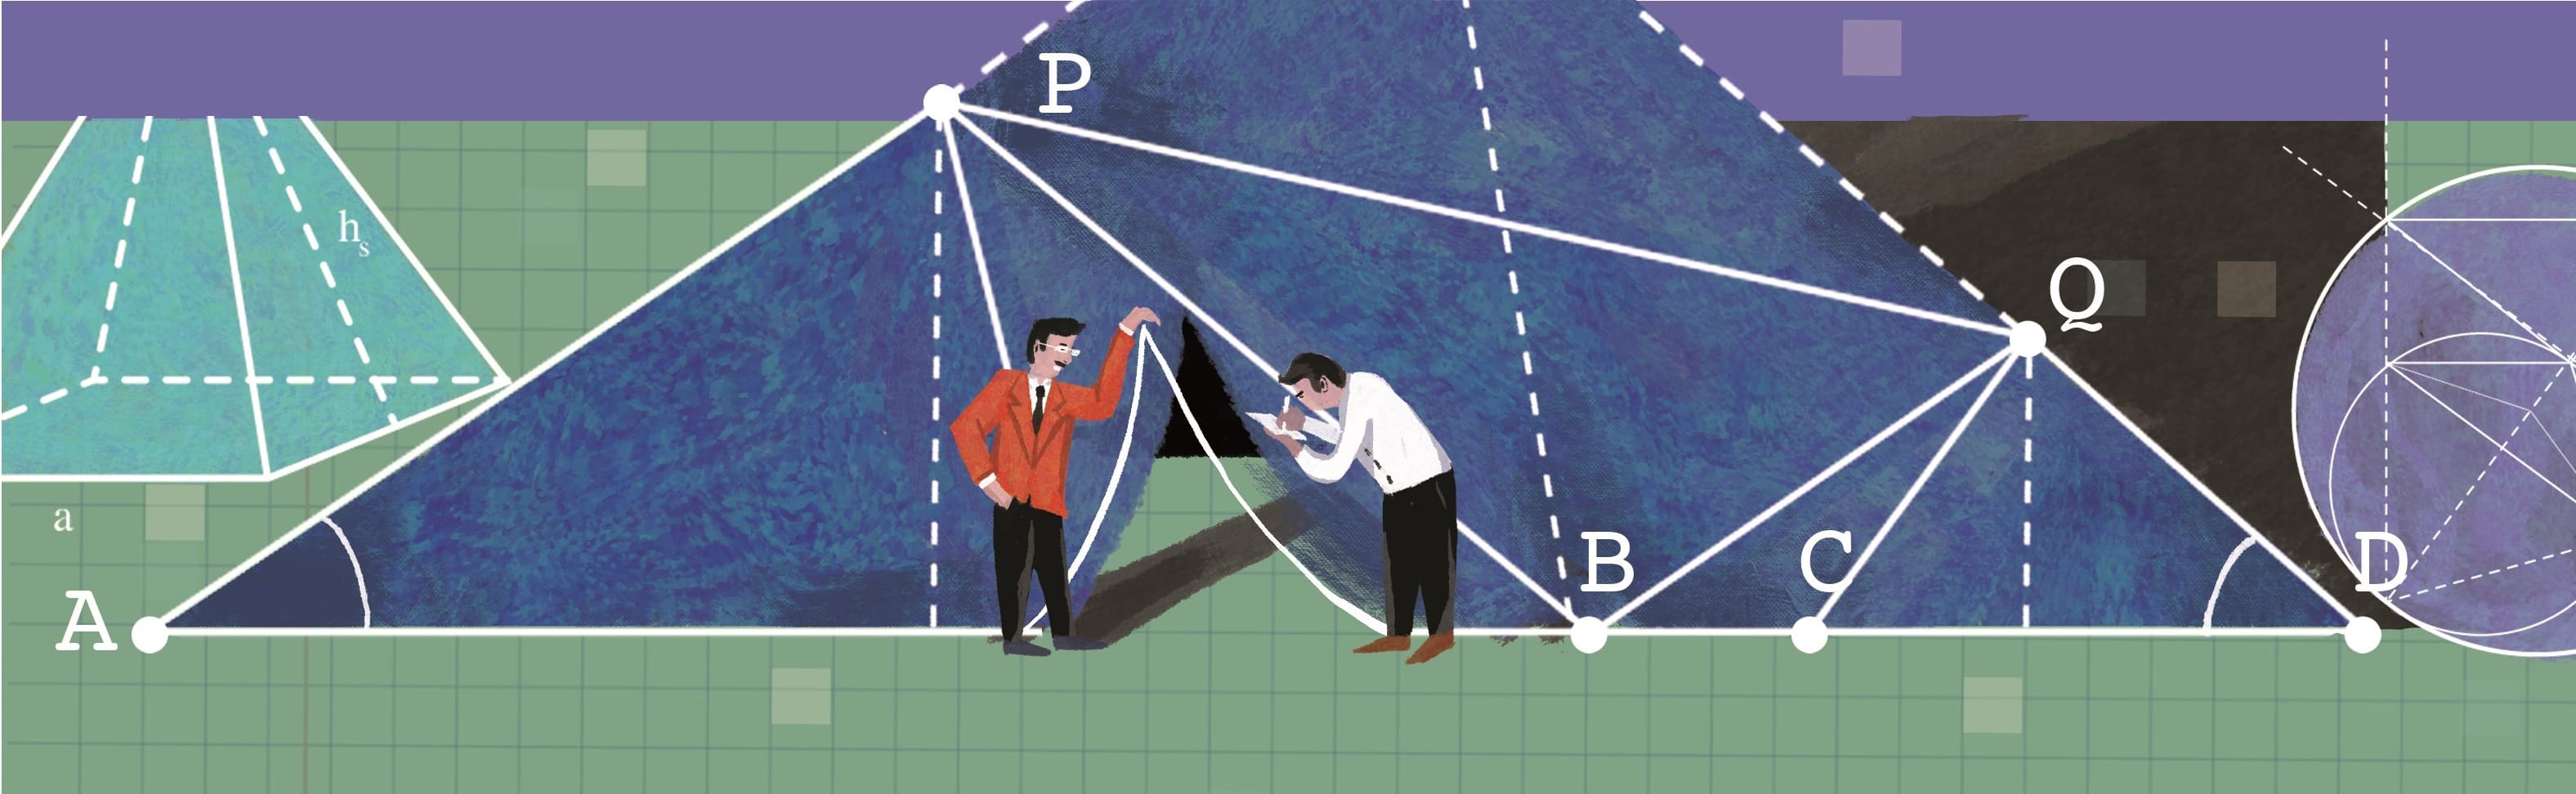
\includegraphics[width=19.3cm]{../bannerhoccungpi}}}
\AddToShipoutPicture*{\put(90,520){
\includegraphics[scale=1]{../tieude.pdf}}}
\centering
\endgroup
\vspace*{185pt}

\begin{multicols}{2}
	Bài toán hai cái can là một loại bài toán rất quen thuộc ở bậc tiểu học. Trong đó, ta cần tìm cách để sử dụng hai cái can với dung tích $a$ và $b$ lít để đong được $k$ lít nước từ bể. Trong bài viết này, chúng ta hãy tìm hiểu mối liên hệ giữa bài toán trên và lý thuyết số.
	\vskip 0.1cm
	$\pmb{1.}$ \textbf{\color{hoccungpi}Bổ đề Bézout và vấn đề tồn tại nghiệm}
	\vskip 0.1cm
	Trong lời giải của bài toán hai cái can nêu trên, ta có những loại thao tác sau:
	\vskip 0.1cm
	$\bullet$ Loại $1$: Đổ đầy một can rỗng hoặc đổ hết nước trong một can đầy trở lại bể
	\vskip 0.1cm
	$\bullet$ Loại $2$: Đổ từ một can đầy sang can rỗng
	\vskip 0.1cm
	$\bullet$ Loại $3$: Đổ toàn bộ nước trong một can (không đầy) sang can rỗng còn lại
	\vskip 0.1cm
	$\bullet$ Loại $4$: Đổ từ một can đầy sang một can đã có một lượng nước nhất định. 
	\vskip 0.1cm
	Trong các loại thao tác trên, lượng nước trong các can sau các thao tác loại $1$ hoặc $2$ đều có thể  biểu diễn bởi các số $a$, $b$ hoặc hiệu của chúng. Thao tác loại $3$ chỉ chuyển vị trí lượng nước. Thao tác loại $4$ bắt đầu từ một trạng thái sau một thao tác loại $4$ khác hoặc từ lượng nước sau một thao tác loại $2$. Do đó, lượng nước ở các can sau thao tác loại $4$ cũng có thể được biểu diễn bằng tổng, và hiệu của nhiều số hạng có giá trị $a$ hoặc $b$. Lượng nước cuối cùng mà ta đong được cũng phải thuộc dạng này.
	\vskip 0.1cm
	Nói cách khác, lượng nước cuối cùng mà ta đong được có dạng theo biểu thức: 
	\begin{align*}
		s\cdot a+ t\cdot b
	\end{align*}
	với $s,t$ là các số nguyên (dạng biểu thức này còn được gọi là một tổ hợp tuyến tính của $a$ và $b$). Để trả lời câu hỏi với các giá trị nào của k thì bài toán có nghiệm, chúng ta sẽ sử dụng bổ đề Bézout trong lý thuyết số.
	\begin{figure}[H]
		\centering
		\vspace*{-5pt}
		\captionsetup{labelformat= empty, justification=centering}
		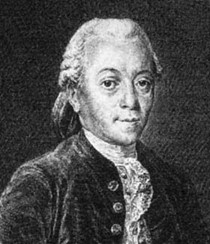
\includegraphics[width=0.75\linewidth]{1}
		\caption{\small\textit{\color{hoccungpi}Étienne Bézout $(1730 - 1783)$.}}
		\vspace*{-10pt}
	\end{figure}
	Bổ đề Bézout (đặt tên theo nhà toán học Pháp, Étienne Bézout ) được phát biểu như sau:
	\vskip 0.1cm
	\textit{Ước chung lớn nhất $d$ của hai số dương $a$ và $b$ luôn có thể được viết dưới dạng $d=s\cdot a+t\cdot b$ với $s,t$ là các số nguyên. Đồng thời, bất kỳ số nguyên nào có dạng $m\cdot a+n\cdot b$ đều là một bội số của $d$.}
	\vskip 0.1cm
	Bổ đề này cho phép ta nhận xét như sau về bài toán hai can nước: với $k$ là số lít nước cần đong, bài toán hai can nước có cách giải khi và chỉ khi $k$ là một bội số của ước chung lớn nhất của $a$ và $b$. Chẳng hạn, với hai can $8$ lít và $12$ lít, do ước chung lớn nhất là $4$ nên ta chỉ có lời giải cho các giá trị cần đong là bội của $4$.
	\vskip 0.1cm 
	Phần sau của bổ đề Bézout có thể được chứng minh một cách dễ dàng từ phần trước. Vì $d$ là ước chung lớn nhất của $a$ và $b$ nên $a=a_0\cdot d$, $b=b_0\cdot d$. Do đó ta luôn có $m\cdot a+n\cdot b=(ma_0+nb_0)\cdot d$.
	\vskip 0.1cm
	Phần trước của bổ đề có một số cách chứng minh khác nhau. Chúng ta hãy cùng tìm hiểu cách chứng minh xuất phát từ thuật toán Euclid. 
	\vskip 0.1cm
	$\pmb{2.}$ \textbf{\color{hoccungpi}Thuật toán Euclid}
	\vskip 0.1cm
	Thuật toán Euclid cho phép chúng ta tìm ước chung lớn nhất của hai số một cách nhanh chóng mà không cần phải tiến hành phân tích ra thừa số nguyên tố. Ban đầu, nó được Euclid phát biểu cho các độ dài đoạn thẳng. Sau đây, chúng ta sẽ mô tả thuật toán này theo ngôn ngữ toán học hiện đại.
	\vskip 0.1cm
	Thuật toán Euclid được xây dựng dựa trên các nhận định sau cho hai số dương $a$ và $b$:
	\vskip 0.1cm
	$\bullet$ $\text{ƯCLN}(a,b) = \text{ƯCLN}(b,a)$					\hfill ($1$)
	\vskip 0.1cm
	$\bullet$ Nếu $a>0$ và $b \,\vdots \,a$ thì $\text{ƯCLN}(a,b) = a$			\hfill ($2$)
	\vskip 0.1cm
	$\bullet$ Nếu $a$ chia cho $b$ dư $c$ thì $\text{ƯCLN}(a,b) = \text{ƯCLN}(c,b)$		\hfill ($3$)
	\vskip 0.1cm
	Hai nhận định đầu tiên ($1$) và ($2$) có thể dễ dàng được chứng minh. Để chứng minh nhận định ($3$), ta sử dụng một số tính chất của phép chia hết. 
	\vskip 0.1cm
	Vì $c$ là số dư trong phép chia cho $b$ nên $a=c+b\cdot y$ với $y$ là một số dương. Gọi $t$ là một ước chung của $b$ và $c$. Do $b\,\vdots\, t$ nên $b\cdot y\, \vdots\,t$. Đồng thời, $c\,\vdots\,t$ nên $a=c+b\cdot y\,\vdots\,t$. Nói cách khác, mọi ước chung của $b$ và $c$ cũng đều là ước chung của $a$ và $b$. 
	\vskip 0.1cm
	Tương tự, khi viết $c=a-b\cdot y$, ta cũng có thể chứng minh mọi ước chung của $a$ và $b$ cũng là ước chung của $b$ và $c$. 
	\vskip 0.1cm
	Do đó, hai tập hợp ước chung này là như nhau nên phần tử lớn nhất của chúng cũng như nhau hay hai cặp số sẽ có chung ước chung lớn nhất.
	\vskip 0.1cm
	Với những nhận định trên, ta có thể tìm ước chung lớn nhất của hai số bằng cách lập một dãy số. Giả sử $a>b$. Đặt $r_0=a,r_1=b$. Sử dụng quy tắc từ ($3$):
	\begin{align*}
		r_{n+1}=r_{n-1}  \mod r_n
	\end{align*}
	(ở đây $\mod$ là toán tử cho ra số dư của phép chia hai số), ta xây dựng được một dãy số giảm dần: $r_0>r_1>r_2>r_3>\cdots$ và do đó sẽ tồn tại một giá trị $N$ sao cho $r_N=0$ (dãy số không thể nhận giá trị âm). Khi đó, $r_{N-2}\,\vdots\,r_{N-1}$. Từ ($2$) và ($3$), ta có $r_{N-1}$ chính là ước chung lớn nhất của hai số ban đầu.
	\vskip 0.1cm
	Ví dụ, với $a=30,b=18$, thuật toán Euclid sinh ra dãy số:
	\begin{align*}
		30&	&&\\
		18&	&&\text{($30$ và $18$ là hai số ban đầu)}\\	
		12&	&&\text{($30$ chia $18$ dư $12$)}\\
		6&	&&\text{($18$ chia $12$ dư $6$)}\\
		0&	&&\text{($12$ chia hết cho $6$)}
	\end{align*}
	và trả về giá trị $6$ (phần tử $r_{N-1}$) cho ước chung lớn nhất.
	\vskip 0.1cm
	Tiếp theo, ta sẽ giải thích xem thuật toán Euclid liên hệ đến bổ đề Bézout như thế nào. Như đã nói ở trên, dãy luôn không âm và giảm dần nên sẽ luôn có giá trị kết thúc $r_N=0$. Đồng thời, ta có thể viết $r_{n+1}=r_{n-1}-q_n r_n$ với $q_n$ là thương số trong phép chia $r_{n-1}$ cho $r_n$. Có thể thấy, mỗi \,phần \,tử của \,dãy là
	\end{multicols}
	\begin{figure}[H]
		\centering
		\vspace*{5pt}
		\captionsetup{labelformat= empty, justification=centering}
		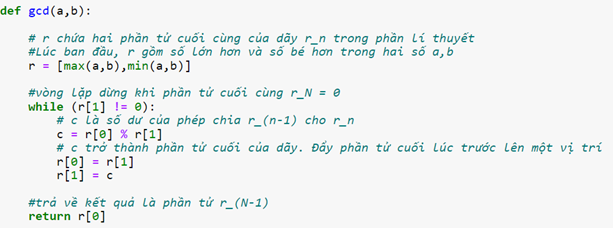
\includegraphics[width=1\linewidth]{2}
		%		\caption{\small\textit{\color{}.}}
		\vspace*{-15pt}
	\end{figure}
	\begin{multicols}{2}
	một tổ hợp tuyến tính của hai phần tử đúng trước nó và do đó cũng là tổ hợp tuyến tính của hai phần tử đầu tiên. Điều này dẫn đến việc ước chung lớn nhất $(r_{N-1})$ mà ta tìm được cũng là một tổ hợp tuyến tính của hai số ban đầu. Đến đây, ta cũng đã chứng minh được phần trước của bổ đề Bézout.
	\vskip 0.1cm
	Ta có thể lập trình một hàm trong Python để tính ước chung lớn nhất sử dụng thuật toán Euclid như trên đây (ý nghĩa của các dòng lệnh được giải thích trong phần comment):
	\vskip 0.1cm
	Khi gọi hàm trên, ta sẽ nhận được kết quả là ước chung lớn nhất của hai số.
	\begin{figure}[H]
		\centering
		\vspace*{-10pt}
		\captionsetup{labelformat= empty, justification=centering}
		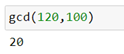
\includegraphics[width=0.4\linewidth]{3}
%		\caption{\small\textit{\color{}.}}
		\vspace*{-15pt}
	\end{figure}
	$\pmb{3.}$ \textbf{\color{hoccungpi}Thuật toán Euclid mở rộng}
	\vskip 0.1cm
	Đến đây thì ta đã giải quyết được vấn đề khi nào bài toán hai can nước có nghiệm. Tuy nhiên, để có thể đưa ra được lời giải cho bài toán, ta cần mở rộng thuật toán Euclid để tính cả các hệ số của tổ hợp tuyến tính biểu diễn ước chung lớn nhất. Với mỗi phần tử $r_n$, ta còn phải tính cả các hệ số $s_n$ và $t_n$ sao cho $r_n=s_n\cdot a+t_n\cdot b$.
	\vskip 0.1cm
	Với hai giá trị đầu của dãy,
	\begin{align*}
		r_0=a=1\cdot a+0\cdot b\\
		r_1=b=0\cdot a+1\cdot b
	\end{align*}
	nên $s_0=1$, $t_0=0$, $s_1=0$, $t_1=1$.
	\vskip 0.1cm
	Đồng thời, do
	\begin{align*}
		r_{n+1}&=r_{n-1}-q_n r_n\\
		&=\left(s_{n\!-\!1}\!\cdot\! a+t_{n-1}\!\cdot\! b\right)-q_n \left(s_n\!\cdot\! a+t_n\!\cdot \!b\right)\\
		&=\left(s_{n-1}-q_n s_n \right)\cdot a+\left(t_{n-1}-q_n t_n \right)\cdot b. 
	\end{align*}
	nên:
	\begin{align*}
		s_{n+1}=s_{n-1}-q_n s_n
		t_{n+1}=t_{n-1}-q_n s_n.
	\end{align*}
	Do ước chung lớn nhất cần tìm là $r_{N-1}$ (khi đã tính ra $r_N=0$), nên ta cũng chỉ cần tính đến $s_{N-1}$ và $t_{N-1}$.
	\vskip 0.1cm
	Ví dụ với $a=48,b=18$ ta có bảng sau:
	\begin{table}[H]
		\vspace*{-5pt}
		\centering
		\captionsetup{labelformat= empty, justification=centering}
		\setlength{\tabcolsep}{8pt}
		\renewcommand{\arraystretch}{1.15}
		\begin{tabular}{|c|c|c|c|c|}
			\hline
			$n$	&$r_n$&	$q_n$&	$s_n$&	$t_n$\\
			\hline
			$0$	&$48$&	&	$1$&	$0$\\
			\hline
			$1$	&$18$&	$2$&	$0$&	$1$\\
			\hline
			$2$&	$12$&	$1$&	$1$&	$-2$\\
			\hline
			$3$&	$6$&	$2$&	$-1$&	$3$\\
			\hline
			$4$&	$0$ & & &\\
			\hline	
		\end{tabular}
		\vspace*{-5pt}
	\end{table}		
	Từ bảng này, ta có ước chung lớn nhất của $48$ và $18$ là $6=-1\cdot 48+3\cdot 18$.
	\vskip 0.1cm
	Đồng thời, kết quả này cũng cho phép ta xác định tổ hợp tuyến tính cho bất kỳ một bội số nào của ước chung lớn nhất. Ví dụ:
	\begin{align*}
		&12=2\cdot 6=-2\cdot 48+6\cdot 18 \\
		&18=3\cdot 6=-3\cdot 48+9\cdot 18 \\
		&\vdots\\
		&72=12\cdot 6=-12\cdot 48+36\cdot 18 \\
		&\vdots
	\end{align*}
	Ta có thể bổ sung vào hàm Python tính ước chung lớn nhất theo thuật toán Euclid để được thuật toán Euclid mở rộng như trong hình dưới:
	\begin{figure}[H]
		\centering
		\vspace*{-5pt}
		\captionsetup{labelformat= empty, justification=centering}
		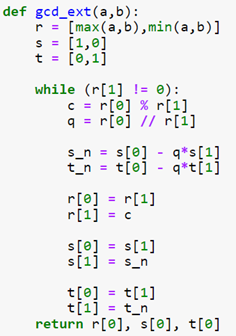
\includegraphics[width=0.75\linewidth]{4}
%		\caption{\small\textit{\color{}.}}
		\vspace*{-10pt}
	\end{figure}
	Ở đây, ta đã thêm hai danh sách $s$ và $t$ để lưu hai phần tử cuối của các dãy $s_n$ và $t_n$ như trong phần lý thuyết. Các giá trị của hai dãy này được tính theo công thức của chúng. Cần lưu ý rằng toán tử // là phép chia cho ra thương số của phép chia có dư. Việc đẩy các giá trị mới vào các danh sách $s,t$ cũng tương tự như với $r$.
	\vskip 0.1cm
	Hàm trên trả ra một bộ ba số gồm ước chung lớn nhất và các tham số s,t gắn với nó.
	\begin{figure}[H]
		\centering
		\vspace*{-5pt}
		\captionsetup{labelformat= empty, justification=centering}
		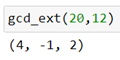
\includegraphics[width=0.4\linewidth]{5}
		%		\caption{\small\textit{\color{}.}}
		\vspace*{-10pt}
	\end{figure}
	Ví dụ với $a=20,b=12,$ ta có: $4=(-1)\cdot 20+2\cdot 12$
	\vskip 0.1cm
	Tổ hợp tuyến tính cho lượng nước cần đong $k$ có thể cho ta cách giải của bài toán hai can nước. Do $k$ sẽ nhỏ hơn giá trị lớn nhất trong hai số $a,b$ nên sẽ luôn có một trong hai hệ số của tổ hợp tuyến tính nhận giá trị âm và hệ số còn lại nhận giá trị dương. Can ứng với hệ số dương là can đầu vào (đổ từ bể vào can) còn can ứng với hệ số âm là can đầu ra (đổ từ can vào lại bể).
	\vskip 0.1cm
	Cách đong của ta được tiến hành như sau:
	\vskip 0.05cm
	$\bullet$ Nếu can đầu vào rỗng thì đổ đầy nó.
	\vskip 0.05cm
	$\bullet$ Nếu can đầu vào không rỗng thì đổ sang can đầu ra cho đến khi nó đầy hoặc can đầu vào hết nước.
	\vskip 0.05cm
	$\bullet$ Nếu can đầu ra đầy thì đổ hết nước bên trong trở lại bể.
	\vskip 0.05cm
	Giá trị tuyệt đối của các hệ số trong tổ hợp tuyến tính sẽ cho ta biết số lần phải đổ đầy can đầu vào cũng như số lần đổ hết nước ở can đầu ra trở lại bể.
	\vskip 0.05cm
	Ta hãy xét trường hợp lượng nước cần đong bằng với ước chung lớn nhất của dung tích hai can. Ví dụ, đong $1$ lít từ hai can $5$ lít và $8$ lít. Thuật toán Euclid cho ta $1=2\cdot 8-3\cdot 5$. Ta có can $8$ lít là can đầu vào còn can $5$ lít là can đầu ra.
	\vskip 0.05cm
	Quy trình đong như sau:
	\begin{table}[H]
		\vspace*{-5pt}
		\centering
		\captionsetup{labelformat= empty, justification=centering}
		\setlength{\tabcolsep}{7pt}
		\renewcommand{\arraystretch}{1.1}
		\begin{tabular}{|l|c|c|}
			\hline
			Bước làm&	Can $8$ lít&	Can $5$ lít\\
			\hline
			Đổ đầy can $8$ lít&	$8$&	$0$\\
			\hline
			Đổ sang can $5$ lít&	$3$&	$5$\\
			\hline
			Đổ hết can $5$ lít&	$3$&	$0$\\
			\hline
			Đổ sang can $5$ lít&	$0$&	$3$\\
			\hline
			Đổ đầy can $8$ lít&	$8$&	$3$\\
			\hline
			Đổ sang can $5$ lít&	$6$&	$5$\\
			\hline
			Đổ hết can $5$ lít&	$6$&	$0$\\
			\hline
			Đổ sang can $5$ lít&	$1$&	$5$\\
			\hline
			Đổ hết can $5$ lít&	$1$	&$0$\\
			\hline
		\end{tabular}
		\vspace*{-10pt}
	\end{table}
	Trong lời giải trên, ta đã đổ đầy can $8$ lít $2$ lần và đổ hết can $5$ lít $3$ lần đúng như các hệ số tương ứng. Nói cách khác, biểu thức theo dạng bổ đề Bézout cho ta một biểu diễn của lời giải bằng một tổ hợp tuyến tính của $a$ và $b$.
	\vskip 0.1cm
	Vậy nếu ta muốn đong một lượng lớn hơn thì sao? Giả sử thay vì $1$ lít, ta muốn đong $2$ lít từ các can trên thì ta sử dụng $2=2\cdot 1=4\cdot 8-6\cdot 5$ và làm tương tự.
	\vskip 0.1cm
	\textbf{\color{hoccungpi}Bài tập}
	\vskip 0.1cm
	$a)$ Hãy lập bảng như trên cho trường hợp đong $2$ lít từ hai can $8$ lít và $5$ lít.
	\vskip 0.1cm
	$b)$ Làm tương tự cho trường hợp muốn đong $4$ lít.
	\vskip 0.1cm
	$\pmb{4.}$ \textbf{\color{hoccungpi}Phương trình Diophantine tuyến tính}
	\vskip 0.1cm
	Quay lại bảng cho trường hợp $1$ lít, ta nhận thấy chỉ cần ngay trong lượt đong đầu tiên, ta đã thu được $3$ lít và lượng nước 6 lít cũng xuất hiện luôn ở cuối lượt đong thứ hai. Trong khi đó, nếu ta giải theo dạng bội của ước chung lớn nhất như cách làm ở phần trước thì số lượt đong sẽ nhiều hơn nhiều ($3=6\cdot 8-9\cdot 5$; $6=12\cdot 8-18\cdot 5$).
	\vskip 0.1cm
	Để giải thích việc này, ta hãy nhìn lại phương trình cần giải cho trường hợp $3$ lít:
	\begin{align*}
		8x+5y=3.	\tag{$4$}
	\end{align*}
	Phương trình trên thuộc dạng phương trình Diophantine tuyến tính: 
	\begin{align*}
		ax+by=c.
	\end{align*}
	Trong các phương trình dạng này, người ta quan tâm đến các nghiệm x,y là số nguyên. Một nghiệm của phương trình đã được cung cấp bằng cách lấy bội của kết quả từ thuật toán Euclid cho hai số $8$ và $5$ như ở trên:
	\begin{align*}
		8\cdot 6+5\cdot (-9)=3
	\end{align*}
	Các phương trình Diophantine được đặt tên theo nhà toán học Hy Lạp, Diophantus. Ông sống ở Alexandria vào khoảng thế kỷ thứ $3$ sau Công nguyên. Các phương trình mà ông nghiên cứu chỉ cho phép các nghiệm là số nguyên. Ngày nay, chúng vẫn là đề tài của nhiều nghiên cứu toán học hiện đại.
	\vskip 0.1cm
	Chúng ta hãy thử tìm xem còn có nghiệm nào khác của phương trình này không. Không mất tính tổng quát, giả sử phương trình còn có nghiệm $x=6+u$, $y=-9+v$ với $u,v$ là các số nguyên. Thay vào phương trình ban đầu ta được:
	\begin{align*}
		8\cdot (6+u)+5\cdot (-9+v)&=3\\
		(8u+5v)+(8\cdot 6-5\cdot 9)&=3\\
		8u+5v&=0		\tag{$5$}
	\end{align*}
	Phương trình ($5$) là phương trình Diophantine thuần nhất (vế phải bằng $0$) tương ứng với phương trình ($4$). Viết lại ($5$) dưới dạng $8u=-5v$, ta thấy vì $8$ và $5$ là hai số nguyên tố cùng nhau nên $u$ phải chia hết cho $5$. Đặt $u=5p$, ta được $v=-8p$ với $p$ là số nguyên. Do $p$ có thể nhận vô số giá trị, phương trình thuần nhất của ta có vô số nghiệm. 
	\vskip 0.1cm
	Phương trình ($4$) cũng sẽ có vô số nghiệm xác định bởi: 
	\begin{align*}
		x&=6+5p\\
		y&=-9-8p.
	\end{align*}
	Chú ý rằng phương trình ($4$) có nghiệm là do vế phải là một bội của ước chung lớn nhất của hai số $8$ và $5$, theo bổ đề Bézout. Trong trường hợp phương trình thuần nhất có hai hệ số không nguyên tố cùng nhau, ta cần chia cả hai vế cho ước chung lớn nhất của hai hệ số rồi tiến hành giải tương tự như trên.
	\vskip 0.1cm
	\textbf{\color{hoccungpi}Bài tập}
	\vskip 0.1cm
	Hãy giải các phương trình nghiệm nguyên sau:
	\vskip 0.1cm
	$a)$ $6x+9y=24$
	\vskip 0.1cm
	$b)$ $4x+12y=44$
	\vskip 0.1cm
	Từ họ nghiệm cho phương trình ($4$), ta hãy nhìn lại trường hợp đong $3$ lít từ hai can $8$ lít và $5$ lít. Ta sẽ có vô số nghiệm để chọn bằng cách thay đổi $p$. Giả sử ta muốn số lần đổ đầy can $8$ lít là ít nhất. Khi đó $p=-1$, ta được nghiệm $x=1$; $y=-1$ hay $8-5=3$ ứng với việc đổ đầy can $8$ lít rồi rót trực tiếp từ can $8$ lít sang can $5$ lít. Trong trường hợp muốn chọn can $5$ lít làm can đầu vào và can $8$ lít làm can đầu ra, ta cần cho y nhận giá trị dương. Giá trị dương nhỏ nhất của $y$ ứng với $p=-2$ hay $x=-4$; $y=7$. Độc giả có thể thử lập bảng các thao tác cho trường hợp này.
	\vskip 0.1cm
	Đến đây, ta đã có thể liệt kê tất cả các lời giải của bài toán hai cái can bằng cách sử dụng thuật toán Euclid mở rộng và giải phương trình Diophantine. Tiếp theo, chúng ta sẽ tìm hiểu một số biến thể của bài toán hai cái can.
	\vskip 0.1cm
	$\pmb{5.}$ \textbf{\color{hoccungpi}Một số biến thể của bài toán hai cái can}
	\vskip 0.1cm 
	Ta hãy xét một bài toán khác cũng với hai cái can. 
	\vskip 0.1cm
	Giả sử có hai bể nước. Bể $1$ đầy nước còn bể $2$ không có nước. Với hai can có dung tích $a$ và $b$ lít, hãy đong $k$ lít từ bể $1$ vào bể $2$.
	\vskip 0.1cm
	Bài toán này cũng quy về giải phương trình Diophantine tuyến tính:
	\begin{align*}
		ax+by=k.
	\end{align*}
	Vẫn theo bổ đề Bézout, bài toán có nghiệm khi $k$ là một bội của ước chung lớn nhất $d$ của $a$ và $b$.
	\vskip 0.1cm
	Khi viết lời giải, ta cần không sử dụng thao tác đong từ can nọ sang can kia mà chỉ cần $s$ lần đong đầy can $a$ và $t$ lần đong đầy can $b$ từ bể $1$ đổ sang bể $2$. Các trường hợp hệ số $s$ hoặc $t$ âm ứng với việc đổ ngược lại từ bể $2$ sang bể $1$.
	\vskip 0.1cm
	Vẫn xét trường hợp hai can $8$ lít và $5$ lít nhưng phải đong $36$ lít sang bể $2$. Từ thuật toán Euclid mở rộng, $8\cdot 2+5\cdot (-3)=1$ nên $8\cdot 72+5\cdot (-108)=36$. Phương trình Diophantine $8x+5y=36$ sẽ có họ nghiệm 
	\begin{align*}
		&x=72+5p\\
		&y=-108-8p
	\end{align*}
	với $p$ là số nguyên.
	\vskip 0.1cm
	Ta hãy nhìn nhận các nghiệm từ khía cạnh thực tế. Nếu cả $x$ và $y$ đều dương thì ta chỉ cần vận chuyển đúng $36$ lít. Nếu có một trong hai giá trị $x$ và $y$ âm thì ta phải đổ nhiều hơn $36$ lít vào bể $2$ và đổ lại phần thừa ra vào bể $1$. Khi đó tổng lượng nước phải vận chuyển sẽ nhiều hơn $36$ lít. Do đó, nếu muốn tiết kiệm công sức, ta chỉ nên xét các nghiệm $x$, $y$ dương. 
	\vskip 0.1cm
	Giải hệ
	\begin{align*}
		72+5p \ge 0\\
		-108-8p\ge 0
	\end{align*}
	ta thấy chỉ có $p=-14$ thỏa mãn. Khi đó $x=2$; $y=4$. Ta cần đổ $2$ lần can $8$ lít và $4$ lần can $5$ lít từ bể $1$ vào bể $2$. Với các giá trị $a,b,k$ khác, có thể có nhiều hơn một giá trị $p$ để cho $x,y$ dương.
	\vskip 0.1cm
	Mặt khác, nếu khoảng cách giữa hai bể là tương đối xa, thì tổng số lượt đi lại có thể quan trọng hơn tổng lượng nước phải vận chuyển do mỗi một lượt ta chỉ có thể vận chuyển một can (giả sử chỉ có một người thao tác). Xét ví dụ $a=9$, $b=2$, $k=34$. Các nghiệm $x,y$ dương của trường hợp này bao gồm: $9\cdot 0+2\cdot 17=34$ và $9\cdot 2+2\cdot 16=34$.
	\vskip 0.1cm
	Trong khi đó, nếu ta chấp nhận nghiệm âm, số lượt phải đi ít nhất khi một trong hai giá trị $x,y$ âm sẽ ứng với nghiệm $9\cdot 4-2\cdot 1=34$. Tuy ta phải vận chuyển tổng cộng $38$ lít nước trong trường hợp này, số lượt di chuyển chỉ có $5$ lượt, ít hơn nhiều so với hai nghiệm nêu trên.
	\vskip 0.1cm
	\textbf{\color{hoccungpi}Bài tập}
	\vskip 0.1cm
	Hãy giải các bài toán sau và tìm phương án với số lần di chuyển hai can ít nhất:
	\vskip 0.1cm
	$a)$ Dùng hai can $6$ lít và $11$ lít đong $51$ lít vào bể $2$.
	\vskip 0.1cm
	$b)$ Dùng hai can $7$ lít và $10$ lít đong $43$ lít vào bể $2$.
	\vskip 0.1cm
	Ta còn có thể mở rộng bài toán ra trường hợp có nhiều can. Để cho đơn giản, ta hãy xét trường hợp sử dụng $3$ can dung tích $a,b,c$ để đong $k$ lít nước từ bể $1$ sang bể $2$, phương trình Diophantine tuyến tính của ta có dạng:
	\begin{align*}
		ax+by+cz=k.
	\end{align*}
	Về điều kiện tồn tại nghiệm của phương trình này, ta cần mở rộng định lý Bézout cho trường hợp $3$ số.
	\vskip 0.1cm
	Gọi $d$ là ước chung lớn nhất của $a$ và $b$. Ta sử dụng thuật toán Euclid mở rộng hai lần: 
	\vskip 0.1cm
	$\bullet$ Biểu diễn $d$ theo $a$ và $b$.
	\vskip 0.1cm 
	$\bullet$ Biểu diễn ước chung lớn nhất $g$ của theo $c$ và $d$ theo hai số này. Hãy nhớ rằng ước chung lớn nhất $g$ của $c$ và $d$ cũng là ước chung lớn nhất của ba số $a,b,c$.
	\vskip 0.1cm
	Thế biểu diễn của $d$ theo $a,b$ vào biểu diễn của $g$ theo $c,d$ để cho ra biểu diễn cuối cùng của $g$ theo $a,b,c$.
	\vskip 0.1cm 
	Theo cách này, ta luôn có thể tìm được biểu diễn của ước chung lớn nhất của ba số theo một tổ hợp tuyến tính của chúng.
	\vskip 0.1cm
	\textbf{\color{hoccungpi}Bài tập}
	\vskip 0.1cm
	$a)$ Chứng minh rằng $\text{ƯCLN}(a,b,c) = \text{ƯCLN}(\text{ƯCLN}(a,b), c)$
	\vskip 0.1cm
	$b)$ Dùng nhận định trên để tìm ước chung lớn nhất của $48$, $72$ và $81$.
	\vskip 0.1cm
	Điều kiện tồn tại nghiệm vẫn là $k$ phải chia hết hết cho ước chung của cả ba số $a,b,c$. Cách chứng minh tương tự như trường hợp bổ đề Bézout cho hai số.
	\vskip 0.1cm
	Để giải phương trình Diophantine cho $3$ số, ta cần tiến hành theo hai bước, mỗi bước giải một phương trình Diophantine cho $2$ số. Cách làm được minh họa cho ví dụ sau:
	\begin{align*}
		8x+6y+7z=20. \tag{$6$}
	\end{align*}
	Trước hết, vì ước chung lớn nhất của $8$ và $6$ là $2$ nên $8x+6y$ sẽ luôn chia hết cho $2$ theo bổ đề Bézout. Do đó, ta đặt $8x+6y=2u$. Thế vào ($6$), ta được:
	\begin{align*}
		2u+7z=20.
	\end{align*}
	Thuật toán Euclid mở rộng cho ta $1=2\cdot (-3)+7\cdot 1$. Do đó $20=2\cdot (-60)+7\cdot 20$. Kết hợp với phương trình thuần nhất ta được:
	\begin{align*}
		&u=-60+7p\\
		&z=20-2p
	\end{align*}
	với $p$ là số nguyên.
	\vskip 0.1cm
	Ta có:
	\begin{align*}
		8x+6y=2u=-120+14p.
	\end{align*}
	Thuật toán Euclid mở rộng cho ta: $2=8\cdot 1+6\cdot (-1)$. Do đó 
	\begin{align*}
		-120+14p&=2\!\cdot\! (\!-\!60\!+\!7p)\\
		&=8\!\cdot\! (\!-\!60\!+\!7p)\!+\!6\!\cdot\! (60\!-\!7p).
	\end{align*}
	Kết hợp với phương trình thuần nhất, ta được:
	\begin{align*}
		x&=-60+7p+6q\\
		y&=60-7p-8q
	\end{align*}
	với $q$ là số nguyên.
	\vskip 0.1cm
	Nghiệm cuối cùng của bài toán có dạng:
	\begin{align*}
		x&=-60+7p+6q\\
		y&=60-7p-8q\\
		z&=20-2p
	\end{align*}
	với $p,q \in \mathbb{Z}$.
	\vskip 0.1cm
	Đến đây ta đã hoàn toàn có thể giải được bài toán cho trường hợp $3$ cái can.
	\vskip 0.1cm
	Cho trường hợp $n>3$ cái can, các chứng minh lý thuyết cùng việc giải phương trình cũng tương tự trường hợp $3$ cái can. Chú ý rằng khi giải phương trình Diophantine tuyến tính cho $n$ ẩn số, ta cần thế từng bước, hai ẩn số một lần.
	\vskip 0.1cm
	\textbf{\color{hoccungpi}Bài tập}
	\vskip 0.1cm
	Hãy giải phương trình nghiệm nguyên sau:
	\begin{align*}
		5x+9y+12z=136.
	\end{align*}
	$\pmb{6.}$ \textbf{\color{hoccungpi}Kết luận}
	\vskip 0.1cm
	Bài toán hai cái can là một bài toán quen thuộc ở bậc tiểu học nhưng đồng thời cũng có những liên hệ thú vị đến các kiến thức phép chia hết và số nguyên tố ở lớp $6$. Tác giả hy vọng bài viết có thể giúp cho việc giảng dạy về lý thuyết số ở bậc trung học cơ sở cho những học sinh muốn tìm hiểu sâu hơn về toán học trở nên dễ dàng hơn.
	\vskip 0.1cm
	\textbf{\color{hoccungpi}Tài liệu tham khảo}
	\vskip 0.1cm
	[$1$] Apostol, T.M. ($2010$). \textit{Introduction to analytic number theory}. New York: Springer.
	\vskip 0.1cm
	[$2$] Titu Andreescu, D Andrica and Ion Cucurezeanu ($2010$). \textit{An introduction to diophantine equations : a problem-based approach}. New York: Birkhäuser.
\end{multicols}
%	\newpage
%	
%	\setcounter{figure}{0}
%	\thispagestyle{cackithitoannone}
\pagestyle{cackithitoan}
\everymath{\color{cackithi}}
\graphicspath{{../cackithi/pic/}}
\blfootnote{{\color[named]{cackithi}$^1$Trường Đại học Mỏ--Địa chất.}}
\begingroup
\AddToShipoutPicture*{\put(0,616){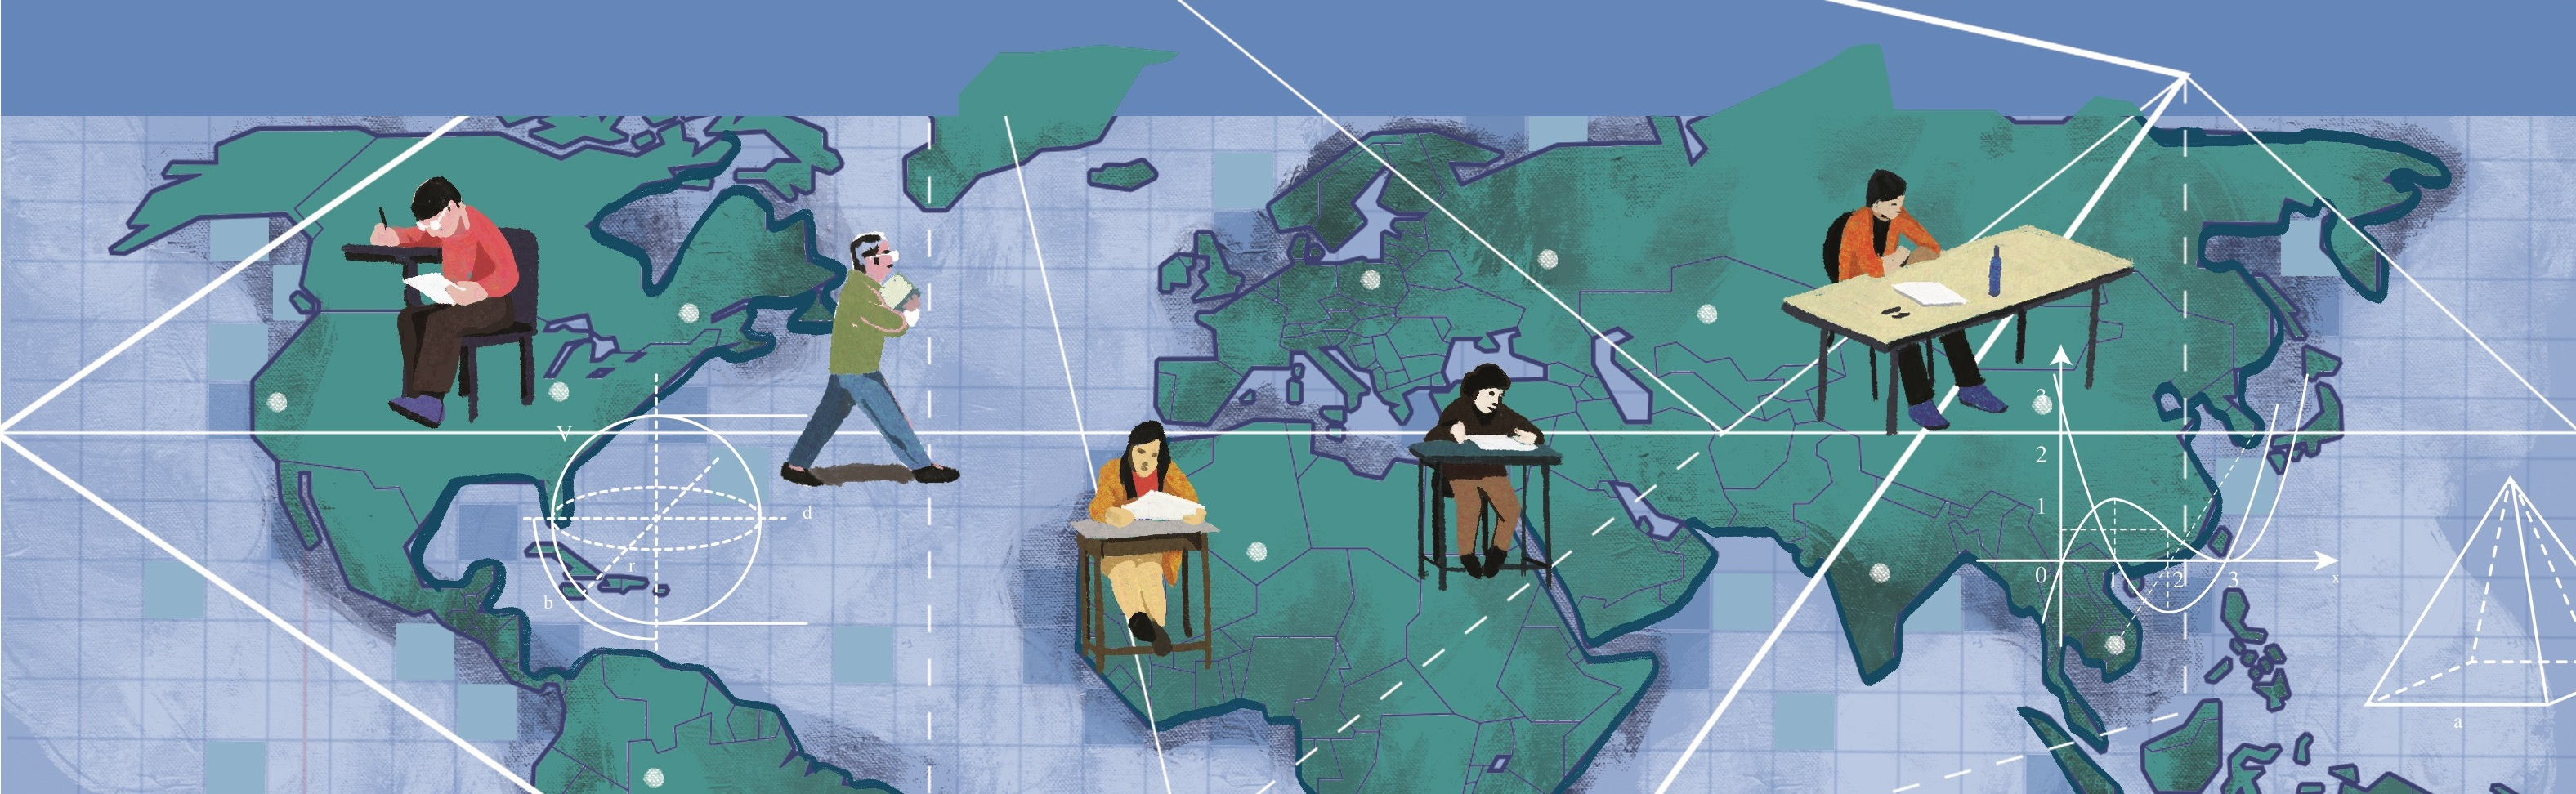
\includegraphics[width=19.3cm]{../bannercackithi}}} 
\AddToShipoutPicture*{\put(64,526){\includegraphics[scale=1]{../tieude3.pdf}}}
\centering
\endgroup
\vspace*{180pt}

%\begin{multicols}{2}
%	Xin được giới thiệu với bạn đọc về kỳ thi ``chinh phục đồi chim sẻ". Đây là kỳ thi do Trường đại học tổng hợp Moscow và nhà xuất bản thanh niên Moscow cùng phối hợp tổ chức từ năm $2005$ nhằm tuyển chọn sinh viên cho trường Đại học tổng hợp Moscow. Xin được nói thêm Trường Đại học tổng hợp Moscow là trường đại học lâu đời nhất và cũng là trường đại học nổi tiếng nhất nước Nga. Nơi đây đã đào tạo ra rất nhiều nhà khoa học danh tiếng. Thi đỗ vào trường là niềm mơ ước của rất nhiều học sinh Nga. Tham gia kỳ thi này là học sinh các lớp từ $9$ tới $11$. Trong đó có kỳ thi riêng dành cho lớp $11$ và cho các bạn lớp $9$ và $10$. Năm $2009$ có $500$ bạn học sinh đã được giải thưởng kỳ thi này và khoảng $400$ bạn đã trở thành sinh viên của trường. Sau đây là bài kiểm tra của năm $2021$.
%	\vskip 0.1cm
%	Kỳ thi ``Chinh phục đồi chim sẻ" năm học $2020/2021$ gồm hai vòng và đều tiến hành thi online. Vòng tuyển loại (diễn ra vào tháng $11-12$ năm $2020$) kéo dài $24$h gồm hai vòng nhỏ hơn: vòng loại có $6$ bài toán và kéo dài $3$ giờ, phần sáng tạo gồm $3$ bài toán và cần phải gửi lời giải trong khoảng thời gian còn lại. Vượt qua vòng tuyển loại, các bạn trẻ sẽ được tham gia vào vòng chung kết diễn ra vào tháng $4$ năm $2021$.
%	\vskip 0.1cm
%	\textbf{\color{cackithi}Vòng loại}
%	\vskip 0.1cm
%	\textit{Mỗi học sinh sẽ nhận được danh sách các bài toán riêng khác biệt. Sau đây là một ví dụ về sáu bài toán của vòng loại.}
%	\vskip 0.1cm
%	$\pmb{1.}$ Giải bất phương trình
%	\setlength{\abovedisplayskip}{5pt}
%	\setlength{\belowdisplayskip}{5pt}
%	\begin{align*}
%		\dfrac{{\sqrt {x + 5}  - x - 3}}{{{x^2} - 15x + 54}} \ge 0
%	\end{align*}
%	Trong đó hãy tìm số lượng nghiệm nguyên của bất phương trình trên.
%	\vskip 0.1cm
%	$\pmb{2.}$ Giải phương trình $\cos 2x + \cos 6x + 2\sin^2 x = 1$.
%	\vskip 0.1cm
%	Trong đó hãy chỉ ra tổng các nghiệm thuộc đoạn $\left[ {\dfrac{{5\pi }}{6};\;\pi } \right]$, làm tròn tới hai chữ số sau dấu phảy.
%	\vskip 0.1cm
%	$\pmb{3.}$ Từ điểm $M$ nằm trong tam giác $ABC$ hạ các đường vuông góc xuống các cạnh $BC$, $AC$, $AB$. Các đường vuông góc này có độ dài tương ứng là $k$, $l$ và $m$. Tìm diện tích của tam giác $ABC$, biết rằng $\angle CAB = \alpha$ và  $\angle ABC = \beta$. Nếu kết quả thu được không là số nguyên, hãy làm tròn nó tới số nguyên gần nhất.
%	\vskip 0.1cm
%	Cho biết các giá trị số là:  $\alpha = \dfrac{\pi}{6}, \beta = \dfrac{\pi}{4},k=3  ,l=2  ,m=4$.
%	\vskip 0.1cm 
%	$\pmb{4.}$ Giải hệ sau
%	\begin{align*}
%		\begin{cases}
%			x^3 + 3y^2 = 11,\\
%			x^2y + xy^2 = 6.
%		\end{cases}
%	\end{align*}
%	Với mỗi nghiệm $(x,y)$ của hệ, hãy tính giá trị của biểu thức $\dfrac{x}{y}$; sau đó tìm giá trị nhỏ nhất trong các giá trị thu được -- lấy xấp xỉ tới hai chữ số sau dấu phảy.
%	\vskip 0.1cm
%	$\pmb{5.}$ Có hai hợp kim. Hợp kim thứ nhất chứa $p\%$ tạp chất, hợp kim thứ hai chứa $q\%$ hợp chất. Hỏi rằng cần phải nung chảy hai hợp kim theo một tỷ lệ nào để thu được một hợp kim mới chứa $r\%$ tạp chất. Trong đáp án khi tính xấp xỉ tỷ lệ khối lượng của hợp kim thứ nhất với khối lượng của hợp kim thứ hai thì làm tròn tới hai chữ số sau \linebreak dấu phảy.
%	\vskip 0.1cm
%	Các dữ liệu số: $p = 70, q = 5, r = 40$.
%	\vskip 0.1cm
%	$\pmb{6.}$ Hãy tìm tất cả các số nguyên $a$ có giá trị tuyệt đối không vượt quá $15$ sao cho bất đẳng thức 
%	\begin{align*}
%		\dfrac{{4x - a - 4}}{{6x + a - 12}} \le 0
%	\end{align*}
%	thỏa mãn với mọi $x$ thuộc khoảng  $[2,3]$. Sau đó hãy tính tổng tất cả các giá trị $a$ vừa tìm được.
%	\vskip 0.1cm
%	\textbf{\color{cackithi}Vòng tuyển chọn (phần sáng tạo)}
%	\vskip 0.1cm
%	$\pmb{7.}$ Tìm tất cả các số tự nhiên $n$ không vượt quá $100$ sao cho tổng ${1^2} + {2^2} + {3^2} + ... + {n^2}$  chia hết cho $50$.
%	\vskip 0.1cm
%	Với những giá trị $n$ vừa tìm được, hãy sắp xếp chúng theo thứ tự tăng dần:  ${n_1} < {n_2} < ... < {n_k}$. Từ đó hãy cho biết $n_{k-2}$ là số nào?
%	\vskip 0.1cm
%	$\pmb{8.}$ Cho trước một đường tròn, trong tất cả các tam giác nội tiếp đường tròn có tổng bình phương của các góc là $\alpha^2 + \beta^2 = \gamma^2 = \dfrac{\pi^2}{2}$ (các góc  $\alpha$,  $\beta$, $\gamma$ được tính bằng radian) hãy tìm tất cả các tam giác có diện tích \linebreak lớn nhất.
%	\vskip 0.1cm
%	Với mỗi tam giác tìm được, hãy tìm giá trị nhỏ nhất của tích các cặp góc. Giá trị nhỏ nhất được làm tròn tới hai chữ số sau dấu phảy. 
%	\vskip 0.1cm
%	$\pmb{9.}$ Hãy tìm tất cả các cặp số dương $x$, $y$ thỏa mãn đẳng thức
%	\begin{align*}
%		&\dfrac{{4{x^2}y + 6{x^2} + 2xy - 4x}}{{3x - y - 2}} \\
%		&+ \sin \left( {\dfrac{{3{x^2} + xy + x - y - 2}}{{3x - y - 2}}} \right)\\
%		= &\,2xy + {y^2} + \dfrac{{{x^2}}}{{{y^2}}} + \dfrac{{2x}}{y} + \dfrac{{2xy({x^2} + {y^2})}}{{{{(3x - y - 2)}^2}}} + \\
%		&+ \dfrac{1}{{{{(x + y)}^2}}}\left( {x^2}\sin \dfrac{{{{(x + y)}^2}}}{x}\right. \\
%		&\left.+ {y^2}\sin \dfrac{{{{(x + y)}^2}}}{{{y^2}}} + 2xy\sin \dfrac{{{{(x + y)}^2}}}{{3x - y - 2}} \right).
%	\end{align*}
%	Trong đáp án hãy viết tổng $x^2 + y^2$ của tất cả các nghiệm  $(x,y)$. Kết quả được làm tròn tới hai chữ số sau dấu phảy. 
%	\vskip 0.1cm
%	\textbf{\color{cackithi}Vòng chung kết}
%	\vskip 0.1cm
%	\textbf{\color{cackithi}Đề $\pmb{1}$}
%	\vskip 0.1cm
%	$\pmb{10.}$ Viết các số tự nhiên bắt đầu từ $20$ thành một dòng: $20212223\ldots$ Hỏi rằng trong dãy kỹ tự thu được, chữ số nào đứng ở vị trí $2021$?
%	\vskip 0.1cm
%	$\pmb{11.}$ Hãy tìm tất cả các giá trị của $a$ sao cho phương trình
%	\begin{align*}
%		|x| \!-\! \arcsin x \!+\! b \!\cdot\! (\arccos x\, \!+\! |x| \!-\! 1) \!+\! a \!=\! 0
%	\end{align*}
%	có ít nhât một nghiệm với mọi giá trị của $b$.
%	\vskip 0.1cm
%	$\pmb{12.}$ Phương trình sau có bao nhiêu nghiệm
%	\begin{align*}
%		{2^{\lg ({x^2} - 3)}} = \lg {2^{{x^2} - 2}}?
%	\end{align*}
%	$\pmb{13.}$ Giải hệ sau
%	\begin{align*}
%		\begin{cases}
%			2x - 3y + \dfrac{1}{xy} = 6,\\
%			3z - 6x + \dfrac{1}{xz} = 2,\\
%			6y - 2z + \dfrac{1}{yz} = 3.
%		\end{cases}
%	\end{align*}
%	$\pmb{14.}$ Gấp một tờ giấy hình vuông có diện tích là $17$ theo đường thẳng đi qua tâm. Sau đó dính các mảnh lại với nhau. Hãy tìm diện tích lớn nhất trong các hình có thể tạo được.
%	\vskip 0.1cm
%	Trong khuôn khổ có hạn của bài báo, chúng tôi chỉ trình bày lời giải chi tiết đối với một số bài chọn lọc.  
%	\vskip 0.1cm 
%	\textbf{\color{cackithi}Đáp án và lời giải}
%	\vskip 0.1cm
%	\textbf{\color{cackithi}Vòng loại}
%	\vskip 0.1cm
%	$\pmb{1.}$ Đáp án: $7$.
%	\vskip 0.1cm
%	$\pmb{2.}$ Đáp án: $2{,}88$ (giá trị chính xác: $\dfrac{11\pi}{12}$).
%	\vskip 0.1cm
%	$\pmb{3.}$ Đáp án: $67$.
%	\vskip 0.1cm
%	$\pmb{4.}$ Đáp án: $-1{,}31$ (giá trị chính xác:  $-\dfrac{1+ \sqrt{217}}{12}$).
%	\vskip 0.1cm
%	$\pmb{5.}$ Đáp án: $1{,}17$ (giá trị chính xác:  $\dfrac{7}{6}$).
%	\vskip 0.1cm
%	$\pmb{6.}$ Đáp án:  $-7$.
%	\vskip 0.1cm
%	\textbf{\color{cackithi}Vòng tuyển chọn (phần sáng tạo)}
%	\vskip 0.1cm
%	$\pmb{7.}$ Đáp án: $87$.
%	\vskip 0.1cm
%	$\pmb{8.}$ Đáp án: $0{,}27$ (giá trị chính xác: $\dfrac{\pi^2}{36}$).
%	\vskip 0.1cm
%	$\pmb{9.}$ Đáp án: $4{,}33$ ($x = \dfrac{9 + \sqrt{17}}{8}$, $y = \dfrac{1+ \sqrt{17}}{4}$ và  $x^2 + y^2 = \dfrac{85 + 13\sqrt{17}}{32} \approx 4{,}33$).
%	\vskip 0.1cm
%	\textbf{\color{cackithi}Vòng chung kết}
%	\vskip 0.1cm
%	\textbf{\color{cackithi}Đề $\pmb{1}$}
%	\vskip 0.1cm
%	$\pmb{10.}$ Đáp án: $7$.
%	\vskip 0.1cm 
%	$\pmb{11.}$ Đáp án:  $\dfrac{\pi}{2} -1$.
%	\vskip 0.1cm 
%	\textit{Lời giải}. Khi  $b = -1$, phương trình có dạng $|x| - \arcsin x - \arccos x - |x| + 1 + a = 0$. Với $x \in [-1;1]$ phương trình tương đương với $1 + a - \dfrac{\pi}{2} = 0$. Như vậy, khi $b = -1$  nghiệm chỉ tồn tại khi $a = \dfrac{\pi}{2} - 1$.
%	\vskip 0.1cm
%	Mặt khác, khi $a = \dfrac{\pi}{2} -1$ phương trình $|x| - \arcsin x + b \cdot (\arccos x\, + |x| - 1) + \dfrac{\pi }{2} - 1 = 0$ có nghiệm $x =1$ với bất kỳ giá trị nào của~$b$.
%	\vskip 0.1cm
%	\textit{Chú thích.} Các bạn thí sinh có nhiều lời giải không đúng vì dựa trên suy luận sau: câu văn từ điều kiện của bài toán ``với mọi giá trị của $b$ có ít nhất một nghiệm" thì bị hiểu nhầm là ``có cùng một nghiệm với mọi trí trị của $b$" (Đây là một bài toán khác, đơn giản hơn mặc dù đáp áp của nó trùng với đáp án của bài toán đã cho). 
%	\vskip 0.1cm
%	$\pmb{12.}$ Đáp án: $4$.
%	\vskip 0.1cm 
%	\textit{Lời giải.} Phương trình được biến đổi về dạng 
%	\begin{align*}
%		{t^\alpha } = \alpha (t + 1),
%	\end{align*}
%	với $\alpha  = \lg 2 \in (0,1)$, $t = {x^2} - 3 > 0$.
%	\vskip 0.1cm
%	Vì vế trái của phương trình $f\left( t \right) = {t^\alpha }$ là hàm lũy thừa với miền xác định $t \ge 0$; và với $\alpha \in  (0,1)$ thì đây là hàm lõm. Trong khi đó vế phải của phương trình $g(t) = \alpha(t+1)$ là hàm tuyến tính với hệ số góc dương nên đồ thị của hai hàm số $f(t)$ và $g(t)$ sẽ cắt nhau tại không quá hai điểm.
%	\vskip 0.1cm
%	Vì $f\left( 0 \right) = 0 < \alpha  = g\left( 0 \right)$ và  $f\left( 1 \right) = 1 = \lg 10 > \lg 4 = 2\alpha  = g\left( 1 \right)$, nên trong khoảng $(0;1)$ tồn tại ít nhất một điểm.
%	\vskip 0.1cm
%	Vì $f(1) > g(1)$, $f\left( {10} \right) = {10^{\lg 2}} = 2 = \lg 100 < \lg {2^{11}} = 11\alpha  = g\left( {10} \right)$, nên trong khoảng $(1;10)$ cũng tồn tại ít nhất một nghiệm.
%	\vskip 0.1cm
%	Điều đó có nghĩa là đồ thị hai hàm số cắt nhau tại đúng hai điểm (một điểm nằm giữa $0$ và $1$, một điểm khác nằm giữa $1$ và $10$).
%	\vskip 0.1cm 
%	Mỗi nghiệm dương $t$ lại sinh ra hai nghiệm $х$ của phương trình đầu. Vì vậy, có cả thảy là $4$ nghiệm.
%	\vskip 0.1cm
%	$\pmb{13.}$ Đáp án:  $x = \dfrac{1}{2}, y = \dfrac{1}{3}, z= 1$  và  $x = -\dfrac{1}{2}, y = - \dfrac{1}{3}  , z= -1$.
%	\vskip 0.1cm 
%	\textit{Lời giải.} Nhân phương trình đầu với  $(2x - 3y)$, phương trình hai với $(3z-6x)$, phương trình thứ ba với $(6y-2z)$. Sau đó cộng chúng lại và thu được phương trình hệ quả:
%	\begin{align*}
%		&{\left( {2x - 3y} \right)^2} + {\left( {3z - 6x} \right)^2} + {\left( {6y - 2z} \right)^2} \\
%		&+ \dfrac{{2x - 3y}}{{xy}} + \dfrac{{3z - 6x}}{{xz}} + \dfrac{{6y - 2z}}{{yz}}\\
%		&= 6\left( {2x \!-\! 3y} \right) \!+\! 2\left( {3z \!-\! 6x} \right) \!+\! 3\left( {6y \!-\! 2z} \right)\\
%		\Leftrightarrow &\,\,{\left( {2x \!-\! 3y} \right)^2} \!+\! {\left( {3z \!-\! 6x} \right)^2} \!+\! {\left( {6y \!-\! 2z} \right)^2} \!=\! 0\\
%		\Leftrightarrow &\,\,2x = 3y = z
%	\end{align*}
%	Thế $2x = 3y = z$ vào hệ, ta được:  $x = \dfrac{1}{2}$, $y = \dfrac{1}{3}$, $z =1$ hoặc $x = - \dfrac{1}{2}$, $y = - \dfrac{1}{3}$,  $z = -1$.
%	\vskip 0.1cm 
%	Chú thích. Dễ dàng nhận thấy là nếu  $2x = 3y = z$, thì tất cả các nhân tử nhân thêm vào phương trình đều bằng $0$. Thế nhưng nó không làm xuất hiện nghiệm ngoại lai vì phương trình tổng vẫn là phương trình hệ quả của hệ đã cho.
%	\vskip 0.1cm
%	$\pmb{14.}$ Đáp án:  $17\left( {2 - \sqrt 2 } \right)$.
%	\vskip 0.1cm 
%	\textit{Lời giải.} Gọi cạnh của hình vuông là $a$. Giả sử đường thẳng cắt và tạo trên cạnh hình vuông $AD$ một đoạn $AP = x < \dfrac{a}{2}$  (Hình $2$).
%	\begin{figure}[H]
%		\vspace*{-5pt}
%		\centering
%		\captionsetup{labelformat= empty, justification=centering}
%		\includegraphics[width= 1\linewidth]{1a.pdf}
%		\caption{\small\textit{\color{cackithi}Hình $2$}}
%		\vspace*{-10pt}
%	\end{figure}
%	Hình vẽ thu được đối xứng qua đường thẳng $PR$. Mặt khác, hình vuông $A_1B_1C-1D_1$ là ảnh của hình vuông $ABCD$ qua phép quay quanh tâm của hình vuông. Khi đó  $x = AP = P{A_1} = {C_1}R = RC = BM = M{D_1}$. Vì vậy các tam giác vuông  $AQP$,  $MBN$,  $NC_1R$, $QD_1M$ là bằng nhau. 
%	\vskip 0.1cm
%	Như vậy diện tích của hình thu được bằng tổng diện tích của hình thang vuông $PD_1C_1R$ và diện tích của hai tam giác vuông bằng nhau  $AQP$,  $MBN$. Diện tích hình thang vuông bằng  $\dfrac{a^2}{2}$. Vì vậy ta cần tìm diện tích lớn nhất của tam giác vuông $AQP$. Chu vi của nó là $AP + AQ + QP = BM + AQ + QM = AB = a$. Trong số các tam giác vuông có chu vi không đổi, thì tam giác vuông cân có diện tích lớn nhất.
%	\vskip 0.1cm
%	Ta sẽ chứng minh khẳng định trên. Gọi $a$, $b$ là các cạnh của tam giác vuông còn $c$ là độ dài của cạnh huyền. Chu vi tam giác là $P = a + b + c$. Sử dụng bất đẳng thức Cauchy có $P = a + b + \sqrt {{a^2} + {b^2}}  \ge 2\sqrt {ab}  + \sqrt {2ab}  = \sqrt {ab} \left( {2 + \sqrt 2 } \right)$. Từ đó suy ra $S = \dfrac{{ab}}{2} \le \dfrac{1}{2}{\left( {\dfrac{P}{{2 + \sqrt 2 }}} \right)^2}$. Đẳng thức xảy ra khi và chỉ khi $a = b$.
%	\vskip 0.1cm 
%	Ta cũng có thể chứng minh khẳng định trên thuần túy bằng hình học: nếu trong góc vuông $ABC$ dựng một đường tròn nội tiếp có bán kính là $\dfrac{P}{2}$, thì đường tròn này sẽ là đường tròn bàng tiếp của tất cả các tam giác vuông có chu vi là $P$ và các cạnh góc vuông $BX$, $BY$ nằm trên hai cạnh của góc. Vì chu vi cho trước, cho nên tam giác có diện tích lớn nhất là tam giác có bán kính đường tròn nội tiếp lớn nhất. Bán kính này đạt giá trị lớn nhất khi đường tròn nội tiếp tiếp xúc với đường tròn bang tiếp (nếu bán kính lớn hơn nữa thì hai đường tròn này sẽ cắt nhau, đó là điều không thể), tức là khi tam giác cân. 
%	Như vậy  $\angle QPA = 45^\circ$, $\angle RPD = \angle QPR = \dfrac{180^\circ - 45^\circ}{2} = 67,5^\circ$. Khi đó $a = AB = 2x + x\sqrt 2 $. Từ đây rút ra được $x = \dfrac{a}{{2 + \sqrt 2 }} = \dfrac{{a\left( {2 - \sqrt 2 } \right)}}{2}$, diện tích tam giác $\Delta QPA$  bằng $\dfrac{{{x^2}}}{2} = \dfrac{{{a^2}\left( {4 + 2 - 4\sqrt 2 } \right)}}{8} = \dfrac{{{a^2}\left( {3 - 2\sqrt 2 } \right)}}{4}$. Điều đó có nghĩa là diện tích cần tìm là $\dfrac{{{a^2}}}{2} + 2 \cdot \dfrac{{{a^2}\left( {3 - 2\sqrt 2 } \right)}}{4} = \dfrac{{{a^2}\left( {1 + 3 - 2\sqrt 2 } \right)}}{2} = {a^2}\left( {2 - \sqrt 2 } \right)$.
%	\vskip 0.1cm 
%	Vẫn tồn tại một lời giải khác hoàn toàn bằng đại số. Giả sử cạnh của hình vuông bằng $a$, đường thẳng cắt cạnh $AD$ của hình vuông một đoạn  $AP = x < \dfrac{a}{2}$. Ta sẽ đi tìm $AQ$. Ký hiệu các góc $\angle RPS = \angle RPQ = \alpha $, $\angle QPA = \beta$. Từ tam giác $PRS$ (với $S$ là hình chiếu của điểm $R$ lên cạnh $AD$), ta tìm được ${\rm{tg}}\,\alpha  = \dfrac{a}{{a - 2x}}$. Do đó  ${\rm{tg}}\,(2\alpha ) = \dfrac{{a(a - 2x)}}{{2x(x - a)}}$,  $AQ = x \cdot {\rm{tg}}\,\beta  = x{\rm{tg}}\,( - 2\alpha ) = \dfrac{{a(a - 2x)}}{{2(a - x)}}$.
%	\vskip 0.1cm
%	Từ đó suy ra, các cạnh của tam giác vuông bằng $x$ và  $\dfrac{{a(a - 2x)}}{{2(a - x)}}$. Khi đó diện tích cần tìm bằng $\dfrac{{{a^2}}}{2} + \dfrac{{ax(a - 2x)}}{{2(a - x)}}$. Bằng cách tính đạo hàm, ta có thể suy ra rằng hàm số $f(x) = \dfrac{{x(a - 2x)}}{{(a - x)}}$  đạt cực đại tại  $x = \dfrac{{a(2 - \sqrt 2 )}}{2}$. Nó tương ứng với các góc  $\beta = \dfrac{\pi}{4}, 2\alpha = \dfrac{3\pi}{4}, \alpha = \dfrac{3\pi}{8}$.
%	%	\vskip 0.1cm
%	%	\textbf{\color{cackithi}Tài liệu tham khảo}
%	%	\vskip 0.1cm
%	%	[$1$] Олимпиада по математике «Покори Воробьевы горы!» -- $2019-2020$ / \textit{Б. А. Будак и др.} // Математика в школе. -- $2021$. -- № 1. С. $28 - 39$.
%	%	\vskip 0.1cm
%	%	[$2$] Олимпиада по математике «Покори Воробьевы горы!» -- $2018-2019$ / \textit{Б. А. Будак и др.} // Математика в школе. -- $2020$. -- № $4$. С. $11 - 23$.
%	%	\vskip 0.1cm
%	%	[$3$] Олимпиада по математике «Покори Воробьевы горы!» -- $2017-2018$ / \textit{Б. А. Будак и др.} // Математика в школе. -- $2018$. -- № $5$. С. $20 - 32$.
%	%	\vskip 0.1cm
%	%	[$4$] Олимпиада по математике «Покори Воробьёвы горы!» -- $2016-2017$ / \textit{Д. В. Горяшин и др.} // Математика в школе. -- $2017$. -- № 8. $С$. $31- 40$.
%	%	\vskip 0.1cm
%	%	[$5$] Олимпиада «Покори Воробьёвы горы!» / \textit{В. В. Галатенко и др.} // Математика в школе. -- $2017$. -- № $2$. С. $12 - 23$.
%	%	\vskip 0.1cm
%	%	[$6$] Олимпиада «Покори Воробьёвы горы!» / \textit{А. С. Зеленский и др.} // Математика в школе. -- $2016$. -- № $4$. С. $10 - 25$.
%	%	\vskip 0.1cm
%	%	[$7$] Олимпиада «Покори Воробьёвы горы!» по математике ($2013 - 2018$) / \textit{А. С. Зеленский и др.} -- М.: МЦНМО, $2019$. -- $192$ С. 
%\end{multicols}
\newpage
\begingroup
\AddToShipoutPicture*{\put(150,697){\includegraphics[scale=1]{../tieude1.pdf}}}
\centering
\endgroup
\vspace*{10pt}

\begin{multicols}{2}
	Trong phần đầu chuyên mục, chúng tôi sẽ trình bày lời giải của các bài toán trong kỳ thi Olympic Toán thành phố Kiev (Ukraina), năm $2022$,   đăng trong số báo $8/2022$. 
	\vskip 0.1cm
	{\bf\color{cackithi} OC$\pmb{19.}$}  Viết phân số $\dfrac{1}{2021}$ thành hiệu của hai phân số tối giản có mẫu số nhỏ hơn.
	\vskip 0.1cm
	\textit{Lời giải.} Chú ý rằng $2021$ là tích của hai số nguyên tố: $2021=43\times 47$.
	\vskip 0.1cm
	Ta cần tìm $a, b$ để $\dfrac{a}{43} - \dfrac{b}{47}= \dfrac{1}{2021}$. Điều này tương đương với $47a-43b=1$. Như vậy $47a\equiv 1 \pmod{43}$, hay $4a\equiv 1\pmod{43}$. Dễ thấy ngay rằng giá trị $a=11$ thỏa mãn. Giá trị tương ứng của $b$ là $12$. Ta có 
	\begin{align*}
		\dfrac{11}{43} - \dfrac{12}{47}= \dfrac{1}{2021}.
	\end{align*} 
	Bằng cách tương tự ta cũng tìm được một cách viết khác 
	\begin{align*}
		\dfrac{35}{47} - \dfrac{32}{43}= \dfrac{1}{2021}.
	\end{align*}
	{\bf\color{cackithi} OC$\pmb{20.}$} Có $n$ tấm thẻ, trên đó viết lần lượt các số thực (không nhất thiết phân biệt): $a_1, a_2, \ldots, a_n $.  Xét tất cả $ 2^n-1 $ cách chọn ra một tập khác rỗng các tấm thẻ và tính tổng các số trên mỗi tập thẻ đã chọn. Hỏi trong số $2^n-1$ tổng nhận được có thể có nhiều nhất bao nhiêu số bằng $1$?
	\vskip 0.1cm
	Ví dụ: với $3$ tấm thẻ có số $-1$, $2$, $2$, thì các tổng thu được là $4$, $3$, $2$, $2$, $1$, $1$, $-1$. Do đó có hai tổng bằng $1$.
	\vskip 0.1cm
	\textit{Lời giải.} Trường hợp cả $n$ số trên thẻ đều bằng $0$ thì không có tổng nào bẳng $1$. Ta chỉ cần xét trường hợp có một số, giả sử là $a_1$ khác $0$. Ta có thể chia tất cả $2^n$ tập con của tập $n$ tấm thẻ thành $2^{n-1}$ cặp bằng cách ghép một tập $A$ không chứa thẻ $a_1$ với tập $A\cup \{\ \text{thẻ chứa}\ a_1\}$. Do trong mỗi cặp hai tổng nhận được có chênh lệch bằng $a_1$ nên chỉ có nhiều nhất một tập có tổng bằng $1$ (quy ước tập rỗng có tổng bằng $0$).
	\vskip 0.1cm
	Như vậy trong mọi trường hợp đều có không quá $2^{n-1}$ tổng bằng $1$. Ta dễ dàng chỉ ra ví dụ có đúng $2^{n-1}$ tổng bằng $1$:  có  $1$ tấm thẻ ghi số $1$, các tấm thẻ khác đều ghi số $0$. Như vậy có thể có nhiều nhất là $2^{n-1}$ tổng bằng $1$.
	\vskip 0.1cm
	{\bf\color{cackithi} OC$\pmb{21.}$} Trong tam giác $ ABC$, đường trung tuyến $BM$ bằng một nửa cạnh $BC$. Chứng minh rằng $ \angle ABM = \angle BCA + \angle BAC$.
	\vskip 0.1cm
	\textit{Lời giải.}
	\begin{center}
		\definecolor{qqwuqq}{rgb}{0.,0.39215686274509803,0.}
		\definecolor{uuuuuu}{rgb}{0.26666666666666666,0.26666666666666666,0.26666666666666666}
		\definecolor{xdxdff}{rgb}{0.49019607843137253,0.49019607843137253,1.}
		\definecolor{ududff}{rgb}{0.30196078431372547,0.30196078431372547,1.}
		\begin{tikzpicture}[cackithi,node font= small]
			\draw [shift={(3.,0.)},color=qqwuqq] (0,0) -- (116.56505117707799:0.5) arc (116.56505117707799:180.:0.5) -- cycle;
			\draw [shift={(2.,2.)},color=qqwuqq] (0,0) -- (-63.43494882292201:0.5) arc (-63.43494882292201:0.:0.5) -- cycle;
			\draw [shift={(4.,2.)},color=qqwuqq] (0,0) -- (180.:0.5) arc (180.:243.43494882292202:0.5) -- cycle;
			\draw [shift={(-1.,0.)},color=qqwuqq] (0,0) -- (0.:0.6) arc (0.:33.690067525979785:0.6) -- cycle;
			\draw [shift={(2.,2.)},color=qqwuqq] (0,0) -- (0.:0.6) arc (0.:33.690067525979785:0.6) -- cycle;
			\draw  (4.,2.)-- (2.,2.);
			\draw  (2.,2.)-- (3.,0.);
			\draw  (2.5849705831449925,1.0983869910099906) -- (2.370308057305012,0.9910557280900002);
			\draw  (2.6296919426949894,1.0089442719099997) -- (2.4150294168550084,0.9016130089900094);
			\draw  (-1.,0.)-- (3.,0.);
			\draw  (-1.,0.)-- (5.,4.);
			\draw  (5.,4.)-- (4.,2.);
			\draw  (4.62969194269499,2.991055728090001) -- (4.415029416855009,3.0983869910099915);
			\draw  (4.584970583144993,2.901613008990009) -- (4.370308057305012,3.0089442719099995);
			\draw  (4.,2.)-- (3.,0.);
			\draw  (3.6296919426949894,0.9910557280900002) -- (3.4150294168550084,1.0983869910099906);
			\draw  (3.584970583144993,0.9016130089900094) -- (3.370308057305012,1.0089442719099997);
			\draw [shift={(-1.,0.)},color=qqwuqq] (0.:0.6) arc (0.:33.690067525979785:0.6);
			\draw[color=qqwuqq] (-0.49752668609324713,0.15213667806142553) -- (-0.35396288211988924,0.1956043003646903);
			\draw [shift={(2.,2.)},color=qqwuqq] (0.:0.6) arc (0.:33.690067525979785:0.6);
			\draw[color=qqwuqq] (2.5024733139067536,2.1521366780614257) -- (2.646037117880111,2.1956043003646903);
				\draw [fill=white] (5.,4.) circle (1.5pt);
				\draw[color=ududff] (5.2,4.33) node {$C$};
				\draw [fill=white] (3.,0.) circle (1.5pt);
				\draw[color=xdxdff] (3.2,-0.31) node {$B$};
				\draw [fill=white] (4.,2.) circle (1.5pt);
				\draw[color=uuuuuu] (4.28,1.97) node {$N$};
				\draw [fill=white] (2.,2.) circle (1.5pt);
				\draw[color=ududff] (1.7,2.35) node {$M$};
				\draw [fill=white] (-1.,0.) circle (1.5pt);
				\draw[color=uuuuuu] (-1.2,-0.23) node {$A$};
		\end{tikzpicture}
	\end{center}
	Gọi $N$ là trung điểm $BC$, ta nối đường trung bình $MN$. Khi đó ta có hai góc so le trong bằng nhau:
	\begin{align*}
		\angle ABM = \angle BMN. \tag{$1$}
	\end{align*}	
	Từ giả thiết ta có $BM= BN$ nên tam giác $BMN$ cân tại $B$.
	\vskip 0.1cm
	Như vậy $\angle BMN =\angle BNM$. \hfill ($2$)
	\vskip 0.1cm
	Từ ($1$) và ($2$) ta nhận được
	\begin{align*}
		\angle ABM= \angle BNM. \tag{$3$}
	\end{align*}
	Mặt khác ta cũng có hai góc đồng vị bằng nhau: $\angle BAC=\angle NMC$. Do đó 
	\begin{align*}
		\angle BNM&= \angle NCM + \angle NMC\\
		&= \angle BCA + \angle BAC. \tag{$4$}
	\end{align*}
	Từ ($3$) và ($4$) ta có đẳng thức cần chứng minh.
	\vskip 0.1cm
	Trong phần cuối của chuyên mục kỳ này, chúng tôi sẽ giới thiệu với bạn đọc các bài toán trong kỳ thi Olympic Toán học vùng Cáp--ca năm $2022$ (Caucasus Math Olympiad). Các bài toán này phù hợp với trình độ học sinh lớp $8-9$.
	\vskip 0.1cm
	{\bf\color{cackithi} OC$\pmb{28.}$} Cho trước các số nguyên dương $a$, $b$, $c$. Biết rằng $\dfrac{c}{b} = \dfrac{b}{a}$, và $b^2 - a - c + 1$ là số nguyên tố. Chứng minh rằng $\dfrac{a}{2}$ và $\dfrac{c}{2}$ là các số chính phương.
	\vskip 0.1cm
	{\bf\color{cackithi} OC$\pmb{29.}$} Cho hình bình hành $ABCD$, các điểm $E$ và $F$ lần lượt nằm trên các đoạn $AD$ và $CD$ sao cho $\angle BCE = \angle BAF.$ Các điểm $K$ và $L$ lần lượt nằm trên các đoạn $AD$ và $CD$ sao cho $AK = ED$ và $CL = FD$. Chứng minh rằng $\angle BKD = \angle BLD$.
	\vskip 0.1cm
	{\bf\color{cackithi} OC$\pmb{30.}$} Peter viết ra $21$ số nguyên dương đôi một phân biệt, mỗi số không lớn hơn $10^6$. Đối với mỗi cặp số $(a, b)$ được Peter viết ra, Nick  viết  số
	\begin{align*}
		F(a, b) = a + b - \gcd (a, b)
	\end{align*}
	trên mảnh giấy của mình (ở đây $\gcd$ ký hiệu ước chung lớn nhất). 
	\vskip 0.1cm
	Chứng minh rằng một trong những số mà Nick viết khác với tất cả những số mà Peter viết. 
\end{multicols}
%	\newpage
%	
%	\setcounter{figure}{0}
%	\thispagestyle{diendandayvahoctoannone}
\pagestyle{diendandayvahoctoan}
\everymath{\color{diendantoanhoc}}
\graphicspath{{../diendantoanhoc/pic/}}
\blfootnote{$^{1}$\color[named]{diendantoanhoc}Tòa soạn Hà Nội, Báo Thanh Niên.}
\begingroup
\AddToShipoutPicture*{\put(0,616){\includegraphics[width=19.3cm]{../bannerdiendan}}}
\AddToShipoutPicture*{\put(56,525){\includegraphics[scale=1]{../tieude.pdf}}}
\centering
\endgroup
\vspace*{195pt}

\textit{\textbf{\color{diendantoanhoc}LTS.} Phan Thành Nam dành giải thưởng của Hội toán học châu Âu năm $2020$. Giải thưởng này được trao bốn năm một lần trong Đại hội Toán học Châu Âu (ECM) cho các nhà khoa học trẻ (không quá $35$ tuổi) nhằm ghi nhận những đóng góp xuất sắc trong lĩnh vực toán học. Nhân dịp Phan Thành Nam về công tác tại Việt Nam, anh đã có những chia sẻ với Pi về con đường học tập của mình.}
\begin{multicols}{2}
	Dù ẵm giải nhì học sinh giỏi văn cấp tỉnh dành cho học sinh THCS nhưng cậu học trò Phan Thành Nam lại ước mơ trở thành nhà vật lý. Vậy là anh quyết tâm thi chuyên toán vì nghe nói muốn hiểu vật lý thì phải giỏi toán. Giấc mơ thưở thiếu thời đó đã dẫn dắt anh đến với giải thưởng chính của Hội toán học châu Âu EMS, bởi những thành tựu dùng toán để giải quyết các vấn đề vật lý lượng tử~...
	\begin{figure}[H]
		\centering
		\vspace*{-5pt}
		\captionsetup{labelformat= empty, justification=centering}
		\includegraphics[width=1\linewidth]{1}
		\caption{\small\textit{\color{diendantoanhoc}GS. Phan Thành Nam tại Viện nghiên cứu cao cấp về Toán. Ảnh: Quang Huy.}}
		\vspace*{-5pt}
	\end{figure}
	\textbf{\color{diendantoanhoc}Ước mơ khởi đầu: trở thành nhà vật lý}
	\vskip 0.1cm
	\textit{Xin chào Phan Thành Nam, anh có thể chia sẻ với Pi về hành trình dẫn anh đến với toán học? Hẳn là anh đã từng là học sinh chuyên toán từ nhỏ, vào ĐH cũng học toán?}
	\vskip 0.1cm
	Đúng là hồi lớp $6$ thì tôi học chuyên toán trường Lương Văn Chánh ở Phú Yên. Gọi là lớp chuyên toán nhưng cũng chỉ khác lớp thường là mỗi tuần chúng tôi được bồi dưỡng thêm vài buổi với nội dung học vượt ra ngoài sách giáo khoa, còn giờ học chính khóa thì cũng học như các bạn lớp thường. Nhưng sau đó mô hình chuyên cấp THCS không còn, lên lớp $7$ tôi trở về học lớp thường. Tôi học đều và thích nhiều môn, năm lớp $9$ còn được giải nhì học sinh giỏi cấp tỉnh môn văn.
	\vskip 0.1cm
	\textit{Ơ, sao tự nhiên anh lại đi thi học sinh giỏi môn văn?}
	\vskip 0.1cm 
	Ban đầu tôi thi học sinh giỏi toán, nhưng bị trượt, không được chọn vào đội tuyển của trường để đi thi tiếp. Vì thế mà cô giáo dạy văn khích lệ tôi thi học sinh giỏi môn văn. Tôi thấy đây là một gợi ý hay, môn văn là môn ``truyền thống" của gia đình tôi, mẹ tôi là giáo viên văn, ba tôi vốn học cử nhân văn ở Trường ĐH Tổng  hợp Huế và sau này làm nhà báo. Trong nhà tôi có rất nhiều sách văn học, lúc rảnh rỗi tôi đọc hết nên cũng rất thích môn văn.  
	\vskip 0.1cm
	\textit{Giải nhì văn cấp tỉnh là một thành tựu ngọt ngào, sao anh không tiếp tục đầu tư cho môn văn mà lại trở thành nhà toán học?}
	\vskip 0.1cm 
	Thật ra khi đó tôi lại ôm ấp một giấc mơ khác, đó là trở thành nhà vật lý. Ấy là do ảnh hưởng của cuốn sách \textbf{\color{diendantoanhoc}\textit{``Các nhà vật lý đi tiên phong"}}, mà hồi đó tôi vừa đọc xong. Tuy nhiên trong sách đó viết rằng để hiểu vật lý thì phải giỏi toán, nên khi vào cấp $3$, tôi chọn thi vào lớp chuyên toán ở Trường THPT chuyên Lương Văn Chánh. 
	\vskip 0.1cm
	\textit{Thi vào đội tuyển toán của trường THCS mà còn bị trượt, vậy mà lại tiếp tục mơ mộng thi vào chuyên toán trường chuyên của tỉnh. Xem ra anh cũng ``liều"?} 
	\vskip 0.1cm
	Đúng là có một chút liều. Nhưng vì nhờ việc trượt đội tuyển toán ở lớp $9$ mà tôi nhận ra mình còn thiếu kiến thức nào để bổ sung trong quá trình ôn thi vào lớp $10$ chuyên toán sau này. Trước đó tôi gần như không học nội dung gì ngoài SGK. Khi ôn thi chuyên toán, tôi mới bắt đầu đào sâu một số nội dung ngoài SGK.
	\vskip 0.1cm
	Thật may là tôi đã đỗ chuyên toán, tuy với mức điểm trung bình nhưng đó là một sự khởi đầu tuyệt vời bởi từ đó tôi được học các thầy dạy toán rất giỏi, họ gieo vào tôi tình yêu, niềm đam mê với toán. 
	\vskip 0.1cm
	\textbf{\color{diendantoanhoc}Học để thỏa mãn đam mê chứ không vì thi thố}
	\vskip 0.1cm
	\textit{Đỗ chuyên toán với mức điểm trung bình, vậy việc học sau đó của anh có chật vật để theo kịp các bạn trong lớp không?}
	\vskip 0.1cm
	Tôi thấy việc học cũng nhẹ nhàng. Cuối năm lớp $10$ tôi còn được chọn đi dự kỳ thi Olympic $30.4$, nhờ đó mà tôi được giao lưu với các bạn học sinh giỏi toán các địa phương khác. Chúng ta vẫn nói về tầm quan trọng của việc được học với các thầy giỏi, nhưng từ trải nghiệm của chính mình, tôi thấy việc được học chung với các bạn giỏi cũng quan trọng không kém. 
	\vskip 0.1cm
	Hồi đó lớp tôi có một bạn rất giỏi, tên là Phùng Trọng Thực (hiện là GV Trường ĐH Bách khoa TP.HCM). Có lần Thực đưa cho tôi một bài toán rất hay và lạ, hỏi có giải được không? Thực cho biết bài toán đó có trong tờ tạp chí Toán học và Tuổi trẻ, đây là lần đầu tôi biết tới tạp chí này. Từ đó, $2$ đứa cùng có thêm một niềm vui chung là ngóng chờ tạp chí \textbf{\color{diendantoanhoc}\textit{Toán học và Tuổi trẻ}} về hàng tháng để ngồi giải bài. Chúng tôi áng chừng thời gian tạp chí về đến Phú Yên (thường chậm hơn thời điểm phát hành ở Hà Nội vài ngày), những ngày đó lảng vảng quanh bưu điện liên tục để hễ tạp chí về đến nơi là mua được ngay. 
	\vskip 0.1cm
	Thời gian đầu, gần như chúng tôi chẳng giải được bài toán nào đăng trong tạp chí đó. Lúc đó chúng tôi mới vào lớp $10$, nhưng có nhiều bài thuộc chương trình lớp $11-12$, nên chúng tôi tự học các kiến thức liên quan trong SGK các lớp trên để có đủ nền tảng cần thiết. Nhờ sự ``máu mê" đó mà chúng tôi bắt đầu giải được bài đầu tiên, rồi bài thứ  hai, thứ ba ...
	\vskip 0.1cm 
	Lên lớp $11$ thì tôi đạt giải nhì HSG quốc gia, được ra Hà Nội thi chọn đội tuyển quốc tế. Có khoảng $40$ bạn dự thi, để chọn ra $6$ bạn. Đề thi rất khó, có những dạng toán tôi chưa gặp bao giờ. Tôi nhớ một kỷ niệm vui là nhờ được mang đồ ăn vào phòng thi, mà tôi có việc để làm lúc thi, tức là tôi chủ yếu ngồi ăn chứ toán thì không làm được bao nhiêu.  
	\vskip 0.1cm
	Lớp $12$ tôi cũng được đi thi quốc gia, nhưng chỉ đạt giải khuyến khích. Lúc đó tôi cảm thấy rất tự tin, vì đã học thêm được rất nhiều kiến thức so với năm lớp $11$, nhưng khi vào phòng thi lại làm bài không tốt.  
	\vskip 0.1cm
	\textit{Không được ``hái quả ngọt" vào năm học lớp $12$ mà anh không nản lòng à, để lại vẫn tiếp tục học toán khi lên ĐH?}   
	\vskip 0.1cm
	Lúc đó tình yêu toán đã bén rễ sâu đậm trong tôi, tôi học là để thỏa mãn đam mê chứ không phải để thi thố. 
	\vskip 0.1cm
	Nhờ đạt giải học sinh giỏi quốc gia, tôi được tuyển thẳng vào ĐH. Lúc đó tôi có nhiều lựa chọn. Ngành CNTT của Trường ĐH Bách khoa TP.HCM là ngành thời thượng. Các trường y dược cũng là mục tiêu phấn đấu của nhiều bạn học sinh giỏi. Còn khoa toán tin Trường ĐH Khoa học tự nhiên, ĐH Quốc gia TP.HCM có điểm chuẩn rất thấp, khoảng $15$ điểm/$3$ môn là đỗ. Tuy nhiên tôi chẳng bận tâm, vì thích toán quá rồi, cứ được học toán tiếp là tôi học. 
	\vskip 0.1cm
	Lúc đó tôi rất thích cuốn sách \textbf{\color{diendantoanhoc}\textit{``Tìm tòi để học giỏi toán"}} của anh Lê Quang Nẫm. Biết anh Nẫm là sinh viên Trường ĐH Khoa học tự nhiên, ĐH Quốc gia TP.HCM, tôi muốn vào đó học, với hy vọng có cơ hội được gặp anh, hoặc được học với các thầy của anh. 
	\vskip 0.1cm
	Anh Lê Quang Nẫm hơn tôi khoảng $5$ tuổi, lúc là học sinh đã rất nổi tiếng. Anh là con nhà nghèo, khi anh trúng tuyển vào lớp $10$ Trường Phổ thông Năng khiếu của ĐH Quốc gia TP.HCM thì ba của anh phải từ Quảng Ngãi vào TP.HCM để đạp xích lô nuôi anh ăn học. Học xong cấp $3$ anh vào khoa Toán tin Trường ĐH Khoa học tự nhiên, và tốt nghiệp thủ khoa. Nhưng đó là những thông tin về sau tôi mới biết. Còn khi đọc cuốn sách của anh Nẫm tôi cảm thấy ngưỡng mộ vì anh viết hấp dẫn quá. 
	\vskip 0.1cm
	\textit{Ba mẹ anh có ý kiến thế nào khi anh chọn học toán?}
	\vskip 0.1cm 
	Ba mẹ tôi dân chủ lắm, chỉ cung cấp thông tin về một số trường/ngành mà ba mẹ nghĩ là tốt, còn quyết định là do tôi. Thật sự lúc đó tôi cũng không mường tượng con đường học Toán ở ĐHKHTN TPHCM là như thế nào. Tôi chỉ nghĩ là có thể nó sẽ giúp mình trở thành giáo viên dạy toán, mà như thế cũng tốt. Thời đó sinh viên tốt nghiệp các ngành khoa học cơ bản mà có chứng chỉ sư phạm là cũng được dạy phổ thông. 
	\vskip 0.1cm
	Đó là một quyết định sáng suốt. Vì khi vào học đại học thì tôi rất may mắn gặp được các thầy giỏi, tâm huyết. Thầy này giúp tôi đến với thầy khác, nhờ thế mà hành trình giúp tôi đến với toán học khá suôn sẻ. 
	\vskip 0.1cm
	\textbf{\color{diendantoanhoc}Dùng toán để hiểu vật lý và khám phá thế giới}
	\vskip 0.1cm 
	\textit{Anh được Hội toán học châu Âu trao giải thưởng chính là bởi thành tựu nào trong nghiên cứu toán học của anh?}
	\vskip 0.1cm 
	Họ xét giải trên cơ sở một cụm công trình, cụ thể là ghi nhận đóng góp của tôi cho lĩnh vực vật lý lượng tử đa hạt. Thông thường trong vật lý lượng tử, để biết tính chất của một hệ thì mình phải giải một phương trình Schrödinger (phương trình đươc đặt theo tên nhà vật lý học người Áo, người đầu tiên thiết lập phương trình này và được giải Nobel vật lý năm $1933$). Nếu hệ chỉ có một hạt, thì phương trình Schrödinger chỉ có một biến trong không gian ba chiều. Nếu hệ có $N$ hạt thì phương trình có $N$ biến, và trong nhiều ứng dụng số lượng biến số rất lớn tới mức mình không thể giải được, kể cả giải chính xác hoặc giải số bằng máy tính. 
%	\vskip 0.1cm
	\begin{figure}[H]
		\centering
		\vspace*{-5pt}
		\captionsetup{labelformat= empty, justification=centering}
		\includegraphics[width=1\linewidth]{3}
		\caption{\small\textit{\color{diendantoanhoc}GS. Phan Thành Nam và một sinh viên. Anh: Quang Huy.}}
		\vspace*{-10pt}
	\end{figure}
	Vì đó là một bài toán rất phức tạp, mình cần sẽ tiếp cận bằng các phương pháp xấp xỉ, thường là thay phương trình tuyến tính nhiều biến bằng phương trình phi tuyến một biến. Đây là phương pháp mà các nhà vật lý học đã phát triển trong một thời gian dài. Câu hỏi đặt ra là làm sao chứng minh được phương pháp xấp xỉ đó là đúng, nghĩa là khi số hạt N tiến về vô cùng thì mô hình xấp xỉ trở thành chính xác. Bằng cách sử dụng và phát triển các công cụ trong toán giải tích, tôi chứng minh được rằng trong những điều kiện cụ thể thì một số mô hình xấp xỉ sẽ đúng với những nguyên lý căn bản trong cơ học lượng tử. 
	\vskip 0.1cm
	\textit{Ở trên anh kể chuyện hồi lớp $9$ anh từng mơ ước trở thành nhà vật lý nên nên mới cố gắng học giỏi toán. Vậy việc sau này anh chọn nghiên cứu sâu về toán trong vật lý lượng tử, việc này có liên quan gì tới ước mơ hồi đó?}
	\vskip 0.1cm 
	Đúng là có liên quan. Sau khi làm thạc sĩ, tôi xin được một số học bổng tiến sĩ khác nhau, có cả toán lý thuyết và toán ứng dụng. Tình cờ trong thời gian này, tôi đọc một cuốn sách rất thú vị là \textbf{\color{diendantoanhoc}\textit{``Lưới trời ai dệt"}} của tác giả Nguyễn Tường Bách. Trong cuốn đó, tác giả trình bày về vật lý lượng tử một cách rất cuốn hút, với nhiều mối liên quan tới triết học Phật giáo. Điều này làm sống lại uớc mơ hồi năm lớp $9$, vốn vẫn quanh quẩn trong tâm trí tôi, đó là học về Vật lý Toán.  
	\vskip 0.1cm
	Vì thế mà tôi chọn GS Jan Philip Solovej ở ĐH Copenhaghen để xin học lên tiến sĩ. Khi đó, tôi vào trang khoa toán tìm các giáo sư, và cảm thấy các công trình nghiên cứu của GS Solovej về vật lý lượng tử là vô cùng hấp dẫn. Mặc dù tôi không hiểu rõ các công trình đó, nhưng cảm thấy các kiến thức toán này nếu cố gắng mình sẽ học được, nên quyết định xin theo thầy. Tôi rất may mắn là được thầy đồng ý. 
	\vskip 0.1cm
	Tôi nghĩ môn vật lý ở chương trình phổ thông là một môn học thú vị, nó giúp cho những đứa trẻ thỏa mãn sự tò mò khi tìm hiểu các hiện tượng tự nhiên. Sau này, nhờ sử dụng các công cụ bên toán mà tôi hiểu được chính xác các khái niệm vật lý, điều này kiến tôi thấy rất sung sướng. Mặc dù có thể đó là những điều nhân loại hiểu ra từ cách đây hàng trăm năm, nhưng khi được đi lại trên con đường khám phá thế giới mà nhân loại đã từng đi, tôi vẫn thấy thật hạnh phúc. 
	\vskip 0.1cm
	\textbf{\color{diendantoanhoc}Sẽ cùng các đồng nghiệp người Việt ở nước ngoài giúp VN lấp khoảng trống vật lý toán...}
	\vskip 0.1cm
	\textit{Anh có biết, ở Việt Nam, có những ai làm việc trong lĩnh vực nghiên cứu của anh không?}
	\vskip 0.1cm 
	Tôi gần như không biết có ai làm về lĩnh vực này ở VN! Có một số nhóm vật lý lý thuyết làm việc trực tiếp với những mô hình xấp xỉ phi tuyến, và một số nhóm vật lý thực nghiệm kiểm tra các mô hình xấp xỉ đó có đúng hay không. Nhưng có vẻ như không có nhà toán học nào nghiên cứu những phương trình nhiều hạt từ các nguyên lý cơ \linebreak bản nhất.  
	\vskip 0.1cm
	\textit{Có nghĩa là lĩnh vực này đang có một khoảng trống lớn ở VN?}
	\vskip 0.1cm 
	Vâng, đúng rồi. Nhưng tôi nghĩ tôi có thời gian để giúp cải thiện việc này. 
%	\vskip 0.1cm
	\begin{figure}[H]
		\centering
		\vspace*{-5pt}
		\captionsetup{labelformat= empty, justification=centering}
		\includegraphics[width=1\linewidth]{4}
		\caption{\small\textit{\color{diendantoanhoc}GS. Phan Thành Nam báo cáo tại Viện Toán học. Ảnh: Viện Toán học.}}
		\vspace*{-10pt}
	\end{figure}
	Đầu tháng $8$ vừa rồi, tôi cùng anh Nguyễn Trọng Toán (GS ở ĐH bang Pennsylvania, Mỹ) tổ chức một trường hè về vật lý toán bên Viện Nghiên cứu cao cấp về Toán (nơi GS Ngô Bảo Châu là Giám đốc khoa học -- PV). Chúng tôi bất ngờ trước sự say mê học hỏi của các bạn trẻ. Trong cả buổi sáng họ nghe chúng tôi giảng bài, tới buổi chiều vẫn kiên trì ngồi lại lớp học làm bài tập. Sau đó tôi dự hội thảo về phương trình đạo hàm riêng kỷ niệm ngày sinh GS Đinh Nho Hào ở Viện toán học VN. Tôi thấy nhiều báo cáo đạt chất lượng rất cao, ngang tầm chất lượng các hội thảo đẳng cấp quốc tế. Điều đặc biệt là có nhiều báo cáo của các bạn trẻ. Do đó, tôi thấy rất lạc quan với sự phát triển của ngành này ở trong nước, và trước mắt tôi có thể dùng các công cụ của ngành phương trình đạo hàm riêng để tương tác với các nhà toán học trong nước. 
	\vskip 0.1cm
	Để xây dựng ngành của mình ở VN, tôi cần phải tiếp tục tổ chức một số trường hè, tổ chức dạy học một số môn học trong các khoa toán của các trường ĐH. Tôi đã trao đổi với một số nhà toán học trong nước và được các anh ủng hộ. Trước hết các thầy trong nước sẽ dạy trước cho sinh viên một số kiến thức tổng quát, sau đó tôi sẽ dạy phần tiếp theo, đi sâu hơn vào lĩnh vực nghiên cứu hiện đại. Bằng các giải pháp đồng thời như trên, tôi hy vọng sẽ có một số bạn trẻ sẽ nảy sinh đam mê về vật lý toán.
	\vskip 0.1cm 
	Một thuận lợi là với riêng ngành giải tích -- phương trình đạo hàm riêng, tôi có nhiều ``đồng minh" là các anh chị người Việt xuất thân từ trường ĐH Khoa học tự nhiên, ĐH Quốc gia TP.HCM và đã đạt được vị trí vững vàng trong các trường đại học hàng đầu trên thế giới. Ở Châu Âu có anh Nguyễn Hoài Minh (GS ĐH Paris Sorbonne ở Pháp); anh Nguyễn Lê Lực (GS ĐH ở Anh); anh Trương Trung Tuyến (GS ĐH Oslo, Na Uy). Ở Mỹ có anh  Nguyễn Trọng Toán (GS ĐH bang Pennsylvania), anh Lê Quang Nẫm (GS ĐH Indiana), anh Trần Vĩnh Hưng (GS ĐH Wisconsin–Madison), anh Phan Văn  Tuộc (GS ĐH Tennessee), anh Trần Minh Bình (GS ĐH Texas A\&M) ... và rất nhiều anh chị khác. Đó là những người trẻ trên dưới $40$ tuổi, đang làm việc rất tích cực, và mọi người đều đồng lòng hướng về VN với mong muốn tham gia vào sự phát triển toán học trong nước.
	\vskip 0.1cm
	\textit{Xin cảm ơn GS Phan Thành Nam!} 
\end{multicols}
\vspace*{-10pt}
\rule{1\linewidth}{0.1pt}

\vspace*{10pt}
\centerline{\LARGE{\textbf{\color{diendantoanhoc}LỜI GIẢI, ĐÁP ÁN}}}
\begin{multicols}{2}
	\textbf{\color{diendantoanhoc}Đố vui}
	\vskip 0.1cm
	Vì không có nhãn nào là đúng, nên sẽ có hai trường hợp:
	\vskip 0.1cm
	-- \textit{Trường hợp} $1$: XĐ có nhãn là XX, XX có nhãn là ĐĐ, ĐĐ có nhãn là XĐ.
	\vskip 0.1cm
	-- \textit{Trường hợp} $2$: XĐ có nhãn là ĐĐ, ĐĐ có nhãn là XX, XX có nhãn là XĐ. 
	\vskip 0.1cm
	Vì vậy chỉ cần $1$ lần bốc, chọn $1$ quả bóng từ hộp XĐ là xác nhận được các bi trong cách hộp.
	\vskip 0.1cm
	\textbf{\color{diendantoanhoc}Góc cờ}
	\vskip 0.1cm
	Đối với những ai có một chút kiến thức về cờ tàn căn bản thì sẽ không mấy khó khăn để tìm ra đáp án trong $2$ hình cờ trên. Nếu đôi bên đi chính xác thì Hình $4$ sẽ có kết quả thắng và Hình $5$ có kết quả hòa, cụ thể như sau: 
	\vskip 0.1cm
	Hình $4$: $\pmb{1)}$ M$6.7$ S$4.5$\quad $2)$ P$9/5$ S$5.4$\quad $3)$ P$9-3$ T$7.9$\quad $4)$ P$3-6$ S$6.5$\quad $5)$ T$5/3$ Tg$-4$\quad $\pmb{6)}$ P$6-7$ T$3.1$ \quad $\pmb{7)}$ M$7/9$. Đen mất Tượng chắc chắn thua cuộc ($1-0$).
	\vskip 0.1cm
	Hình $5$: $\pmb{1)}$ M$7/8$ S$5.6$\quad $\pmb{2)}$ T$7/5$ S$s.5$\quad $\pmb{3)}$ S$6/5$ P$4.5$\quad $\pmb{4)}$ P$9.4$ P$4-8$\quad $\pmb{5)}$ M$8.7$ Tg$-4$\quad $\pmb{6)}$ P$9-5$ P$8/3$\quad $\pmb{7)}$ M$7/6$ P$8/2$\quad $\pmb{8)}$ T$5/7$ T$5/3$\quad $\pmb{9)}$ T$3/5$ P$8-6$\quad $\pmb{10)}$ M$6/8$ T$3.5$\quad $\pmb{11)}$ M$8.6$ P$6-7$\quad $\pmb{12)}$ P$5-6$ Tg$-5$\quad $\pmb{13)}$ P$6-4$ T$5/3$. Mặc dù Đỏ hơn quân nhưng Đen phòng thủ vô cùng chắc chắn, hòa cuộc ($1/2$).
	\vskip 0.1cm
	\textbf{\color{diendantoanhoc}Ông chủ quán kỳ lạ}
	\vskip 0.1cm
	Các em thấy ngay để xác định được đường đi, Xuân Phong phải đưa ra câu hỏi không chỉ chứa thông tin của con đường mà còn chứa cả thông tin cần biết về chính ông chủ quán nước.
	\vskip 0.1cm
	\hfill(\textit{Xem tiếp trang} $63$.)
\end{multicols}
%	\newpage
%	
	\setcounter{figure}{0}
	\thispagestyle{lichsutoanhocnone}
\pagestyle{lichsutoanhoc}
\graphicspath{{../lichsutoanhoc/pic/}}
\everymath{\color{lichsutoanhoc}}
\blfootnote{$^1$\color{lichsutoanhoc}Cộng tác viên Viện Toán học.}
\begingroup
\AddToShipoutPicture*{\put(0,616){\includegraphics[width=19.3cm]{../bannerlichsu}}}
\AddToShipoutPicture*{\put(100,515){\includegraphics[scale=1]{../tieude.pdf}}}
\centering
\endgroup

\vspace*{200pt}

\begin{multicols}{2}
	\textbf{Lời dẫn:} Tiếp thu những thành tựu thiên văn học và toán học của người Babylon và người Ai Cập, người Hy Lạp đã đẩy toán học lên thành một ngành khoa học độc lập, với các triết lí và phương pháp riêng. Toán học Hy Lạp đã phát triển rực rỡ trong $1000$ năm, từ năm $600$ trước Công nguyên đến năm $400$ Công nguyên. Người đặt nền móng cho toán học Hy Lạp là nhà toán học, thiên văn học và triết học Thales. Ông là người đứng đầu và là nhà toán học duy nhất trong \textit{Bảy nhà thông thái Hy Lạp} (Seven Sages of Greece).
		\begin{figure}[H]
		\centering
		\vspace*{-5pt}
		\captionsetup{labelformat= empty, justification=centering}
		\includegraphics[width=1\linewidth]{1}
		\caption{\small\textit{\color{lichsutoanhoc}Hình $1$: Bảy nhà thông thái Hy Lạp.}}
		\vspace*{-10pt}
	\end{figure}
	\textbf{Tiểu sử}
	\vskip 0.1cm
	Thales (khoảng $625 - 547$ trước Công nguyên) là người gốc Phoenicia, sinh ra ở Miletus, một thành phố của Ionia, khi đó thuộc Hy Lạp, hiện nay thuộc Thổ Nhĩ Kỳ. 
		\begin{figure}[H]
		\centering
		\vspace*{-5pt}
		\captionsetup{labelformat= empty, justification=centering}
		\includegraphics[width=1\linewidth]{2}
		\caption{\small\textit{\color{lichsutoanhoc}Hình $2$: Bản đồ đế chế Hy Lạp.}}
		\vspace*{-10pt}
	\end{figure}
	Hồi trẻ ông theo nghề buôn. Ông được coi là người sắc sảo và thông minh trong nghề. Và trong các chuyến đi của mình, Ông đã học toán từ người Ai Cập và thiên văn từ người Babylon.
	\vskip 0.1cm
	\textbf{Thales -- nhà toán học} 
	\vskip 0.1cm
	Toán học Ai Cập về cơ bản là tập hợp các công cụ và kĩ thuật được định hình để giải các bài toán thực tế. Dựa trên những nguyên liệu thô nhưng phong phú này của người Ai Cập, người Hy Lạp đã tái tạo lại thành các nguyên tắc chung, qua đó làm cho kiến thức toán học trở nên tổng quát và dễ hiểu hơn, đồng thời khám phá ra nhiều điều mới. Thí dụ, “diện tích cánh đồng ngũ cốc hình tam giác” cụ thể đã được trừu tượng và tổng quát thành “diện tích hình tam giác”.
		\begin{figure}[H]
		\centering
		\vspace*{-5pt}
		\captionsetup{labelformat= empty, justification=centering}
		\includegraphics[width=0.65\linewidth]{3}
		\caption{\small\textit{\color{lichsutoanhoc}Hình $3$:  Thales (Khoảng $625 - 547$ trước Công nguyên).}}
		\vspace*{-10pt}
	\end{figure}
	\textbf{Phương pháp suy diễn}
	\vskip 0.1cm
	Thales được công nhận là người đầu tiên chứng minh các khẳng định toán học nhờ logic dựa trên lập luận suy diễn thay cho thực nghiệm và trực giác. Nhà triết học Proclus (khoảng $412 - 485$) trong cuốn \textit{Commentary on the First Book of Euclid’s Elements}  (Chú giải cuốn sách \textit{Cơ sở}  của Euclid) đã viết: \textit{“Thales là người đầu tiên  đưa hình học Ai Cập vào Hy Lạp. Ông còn tự mình tìm ra nhiều mệnh đề [...], trong một số trường hợp, các phương pháp của ông là tổng quát, trong những trường hợp khác mang tính thực nghiệm.”}
	Thales đã đóng góp cho hình học những định lý sau đây, được đưa vào \textit{Cơ sở} của Euclid:
	\vskip 0.1cm
	$1)$  Hai đường thẳng cắt nhau tạo nên các góc đối đỉnh bằng nhau.\footnote[2]{Mệnh đề $I.15$, $[1]$ trang $131$; $[6]$ trang $41$.}
	\vskip 0.1cm
	$2)$  Đường tròn bị chia làm hai phần bằng nhau bởi đường kính của nó.\footnote[3]{$[1]$, trang $131$}
	\vskip 0.1cm 
	$3)$ Góc nội tiếp chắn nửa đường tròn là góc vuông.\footnote[4]{$[1]$, trang $131$}
	\vskip 0.1cm 
	$4)$ Hai góc ở đáy của tam giác cân bằng nhau.\footnote[5]{Mệnh đề $I.5$, $[1]$, trang $131$ hoặc $[6]$, trang $27$}
	\vskip 0.1cm
	$5)$ Các cạnh của hai tam giác đồng dạng tương ứng tỉ lệ.\footnote[6]{Mệnh đề $VI.4$, $[1]$ trang $131$; $[6]$, trang $294$} 
	\vskip 0.1cm
	$6)$ Hai tam giác bằng nhau nếu chúng có một cạnh và hai góc kề với nó tương ứng bằng nhau. \footnote[7]{Mệnh đề $I.26$, $[1]$ trang $131$; $[6]$, trang $56$).
	\vskip 0.1cm 
	Định lí đảo của Định lí $3)$ cũng đúng. Định lí $3)$ có nhiều ứng dụng. Dưới đây là hai Thí dụ.
	\vskip 0.1cm
	\textbf{Thí dụ} $\pmb{1.}$ \textit{Xác định tâm hình  tròn nhờ sử dụng một thước thợ (thước vuông) và một thước thẳng.}
	\vskip 0.1cm
	\textbf{Lời giải:}
	\textbf{Bước $\pmb{1}$:} Đặt đỉnh của thước vuông trên đường tròn. Hai cạnh của thước vuông cắt đường tròn tại hai điểm. 
	\vskip 0.1cm
	\textbf{Bước $\pmb{2}$:} Lấy thước kẻ nối hai điểm vừa nhận được. Đây chính là một đường kính của đường tròn. 
	\vskip 0.1cm
	\textbf{Bước $\pmb{3}$:} Đặt đỉnh thước thợ vào một điểm khác và làm lại Bước $1$ và Bước $2$, được đường kính thứ hai. Giao của hai đường kính chính là tâm đường tròn (Hình $4$). 
	\begin{figure}[H]
		\centering
		\vspace*{-5pt}
		\captionsetup{labelformat= empty, justification=centering}
		\includegraphics[width=1\linewidth]{4}
		\caption{\small\textit{\color{lichsutoanhoc}Hình $4$: Xác định tâm hình tròn.}}
		\vspace*{-10pt}
	\end{figure}
	\textbf{Thí dụ $\pmb{2}$.} Từ một điểm $P$ cho trước kẻ tiếp tuyến tới đường tròn tâm  $O$ cho trước.
	\vskip 0.1cm
	\textbf{Lời giải:} Đường tròn đường kính $OP$  cắt đường tròn tâm $O$  tại hai điểm $T$   và $T'$.  Khi ấy $PT$  và $PT'$  là hai tiếp tuyến cần tìm (Hình $5$).
	\begin{figure}[H]
		\centering
		\vspace*{-5pt}
		\captionsetup{labelformat= empty, justification=centering}
		\includegraphics[width=1\linewidth]{5}
		\caption{\small\textit{\color{lichsutoanhoc}Hình $5$: Kẻ tiếp tuyến tới đường tròn.}}
		\vspace*{-10pt}
	\end{figure}
	Đóng góp quan trọng nhất của Thales trong toán học là ông đã đưa ra một phương pháp chứng minh thống nhất: phương pháp suy diễn logic, tức là từ giả thiết, nhờ một dãy các suy luận logic dựa trên những điều đã được công nhận (các định nghĩa và tiên đề) và các điều đã được chứng minh (các định lí và mệnh đề), dẫn đến điều cần chứng minh. Điều này đã giúp người Hy Lạp đưa toán học, đặc biệt là hình học lên một tầm cao mới, thành một hệ thống chặt chẽ và thống nhất. Do đó, nhiều học giả coi Thales là \textit{nhà hình học đầu tiên} và định lí \textit{Một đường thẳng song song với cạnh đáy của tam giác tạo ra một tam giác mới có các cạnh tỉ lệ với các cạnh của tam giác cũ} (Hình $6$) được mang tên \textit{Định lí Thales}.
	\vskip 0.1cm
	\textbf{Giả thiết:} $BC \parallel B'C'$.
	\vskip 0.1cm    
	Kết luận: $\frac{AB}{AB'} = \frac{AC}{AC'} = \frac{BC}{B'C'}$.
	\vskip 0.1cm
	Tỉ lệ trên vẫn được bảo toàn khi ta tịnh tiến hoặc quay tam giác $ABC$ (Hình $6$, bên phải). Tức là, \textit{nếu hai tam giác có các góc bằng nhau, thì các cạnh của chúng tương ứng tỉ lệ}. Các tam giác như vậy được gọi là \textit{tam giác đồng dạng}.
	\begin{figure}[H]
		\centering
		\vspace*{-5pt}
		\captionsetup{labelformat= empty, justification=centering}
		\includegraphics[width=1\linewidth]{6}
		\caption{\small\textit{\color{lichsutoanhoc}Hình $6$: Định lí Thales.}}
		\vspace*{-10pt}
	\end{figure}
	Christopher Clavius (1538-1612) và  François Viète (1540-1603) đã phát triển khái niệm tam giác đồng dạng của Thales thành khái niệm hình đồng dạng:. 
	
	Hình 7: Hình đồng dạng phối cảnh.
	Hai hình   và   được gọi là đồng dạng (phối cảnh) với nhau theo tâm     tỉ số   nếu với mỗi điểm    có thể tìm được điểm   (và ngược lại, với mỗi điểm    có thể tìm được điểm  ) sao cho  
	Từ Định lí Thales suy ra, nếu các hình   và   và   đồng dạng phối cảnh với nhau tâm   tỉ số   thì với mỗi cặp điểm, thí dụ,  , có thể tìm được các cặp điểm   và  sao cho  
	và  
	Tương tự,    (Hình 7).
	
	Ứng dụng tam giác đồng dạng 
	đĐĐo chiều cao của Đại Kim tự tháp 
	Có hai giai thoại nói về chuyện Thales đã đo chiều cao của Đại Kim tự tháp. Giai thoại thứ nhất kể rằng Thales đã cắm một cây gậy dưới bóng nắng mặt trời. Khi bóng của cây gậy dài bằng chiều cao của nó, ông đo bóng của kim tự tháp và suy ra chiều cao của nó. Giai thoại thứ hai do nhà thơ, nhà viết sử Hy Lạp Plutarch  (46 - -120) viết trong tác phẩm Convivium (Bữa tiệc): “Mặc dù ông ta [Vua Hy Lạp] ngưỡng mộ anh [Thales] về rất nhiều điều, nhưng ông đặc biệt ngưỡng mộ anh bởi cái cách anh đo Đại Kim tự tháp mà không cần dụng cụ nào.”
	
	Hình 8: Đại Kim tự tháp Giza (Cheops).
	Cả hai giai thoại đều dựa trên một mệnh đề hình học (của Thales): Hai tam giác có các góc tương ứng  bằng nhau (nói cách khác, hai tam giác đồng dạng) thì các cạnh của chúng tương ứng tỉ lệ. Tức là:    
	,
	trong đó    và    là chiều cao và chiều dài bóng (tính từ tâm) của kim tự tháp, còn    và    là chiều cao và chiều dài bóng của cây gậy (xem Hhình bên 9dưới). 
	Thales đã biết cạnh đáy của Đại Kim tự tháp   foot nên khoảng cách từ tâm kim tự tháp ra đến cửa bằng    foot. Cây gậy dài 6 foot, bóng của cây gậy bằng 9 foot. Khoảng cách từ cửa đến bóng của đỉnh Kim tự tháp bằng 342 foot. Suy ra  foot. Vậy chiều cao kim tự tháp là 
	foot.
	Hình 9: Đo chiều cao Đại Kim tự thápThales đã biết cạnh đáy của Đại Kim tự tháp bằng.  foot (1 foot = 0,3048 m) nên khoảng cách từ tâm kim tự tháp ra đến cửa bằng  foot. Cây gậy dài 6 foot, bóng của cây gậy bằng 9 foot. Khoảng cách từ cửa đến bóng của đỉnh Kim tự tháp bằng 342 foot. Suy ra foot. Vậy chiều cao kim tự tháp là foot.
	
	
	
	Đo khoảng cách tới tàu biển 
	Một ứng dụng khác của tam giác đồng dạng là đo khoảng cách từ bờ tới tàu đang ở ngoài biển. 
	
	Hình 10: Tính khoảng cách đếên tàu.
	Giả sử    là vị trí của tàu,  tháp có đáy là điểm  chiều cao tháp là   chiều cao của người quan sát đứng trên đỉnh tháp có chiều cao là là    điểm   (mắt người), vị trí   của tàu và điểm  thẳng hàng,     là các khoảng cách có thể đo được và điểm   (mắt người), vị trí   của tàu và điểm   thẳng hàng. Từ hai tam giác đồng dạng    và     ta có  :  Suy ra khoảng cách
	từ bờ tới tàu bằng   
	Một cách khác để đo khoảng cách từ điểm   trên bờ biển tới con tàu   là dựng một đoạn   trên bờ biển vuông góc với  Mắt người đặt ở điểm  trên đường vuông góc với   tại   Đường thẳng   cắt  tại   Như vậy,   thẳng hàng.Từ hai tam giác vuông đồng dạng   và   ta có   
	Vì      đo được nên  (Hình 11)
	
	
	Hình 11: Tính khoảng cách đến tàu, đồn địch
	Bài toán trên còn được áp dụng trong quân sự, khi cần đo khoảng cách từ trận địa pháo đến điểm  là đồn địch (điểm không tới được).
	Thales - nhà thiên văn 
	Đương thời, Thales nổi tiếng là một nhà thiên văn hơn là một nhà toán học. Ông đã tính được một năm có 365 ngày. Ông giải thích hiện tượng nhật thực diễn ra là do mặt trăng che khuất mặt trời. Một truyền thuyết hay được nhắc lại là người Hy Lạp rất ngạc nhiên khi Thales đã tiên đoán đúng nhật thực vào ngày 28 tháng 5 năm 585 trước Công nguyên. Nhà sử học Hy Lạp Herodotus (khoảng 484 - 425 trước Công nguyên) đã ghi lại rằng sự kiện này diễn ra trong một trận chiến giữa người Lydia và người Media. Và khi ngày chuyển sang đêm (do nhật thực), cuộc chiến chấm dứt. Các vị vua đã kinh hoàng đến mức họ đã kí kết một nền hòa bình lâu dài.
	
	Một số giai thoại vui về Thales 
	Mọi người đều nhất trí đánh giá Thales là một người sắc sảo và thông minh không chỉ trong khoa học, mà cả trong chính trị và thương mại. Nhiều giai thoại, một số là nghiêm túc, một số là huyền ảo, kể về sự thông minh của ông. Dưới đây là một vài giai thoại về Thales.   
	
	Chuyện buôn ô liu 
	Theo Aristotle (nhà triết học và bác học Hy Lạp, 384 - 322 trước Công nguyên), có một lần, sau nhiều năm liền cây ô liu không ra quả. B, bằng kiến thức thiên văn của mình, Thales đã dự đoán mùa tới sẽ bội thu. Ông liền mua tất cả các máy ép ô liu xung quanh Miletus, quê ôÔng. Khi mùa thu hoạch đến, do có độc quyền quản lí máy ép, ông đã đưa ra giá thuê chúng theo ý ông, và do đó đã thu được một khoản tiền lớn. Một số người cho rằng, Thales muốn chứng minh quan điểm của mình là, các triết gia, nếu họ muốn, rất dễ trở nên giàu có.
	Chuyện buôn muối 
	Thales có một đàn la chở muối đi bán. Ông tình cờ quan sát thấy một số con la dìm mình xuống nước khi qua suối, do đó muối bị tan ra và la được chở nhẹ hơn. Lần sau, ông cho những con la đó chở những tấm bọt biển. Khi la dìm mình xuống nước, bọt biển thấm nước làm la phải chở nặng hơn. Từ đó trở đi, la thông minh không dám dìm mình xuống nước nữa.
	
	Chuyện mải ngắm sao vấp ngã 
	
	Theo Plato (nhà triết học Hy Lạp, khoảng 424 - 348 trước Công nguyên), một lần vào buổi đêm, Thales ra ngoài đi dạo, do mải ngắm sao, ông đã ngã xuống một con mương. Một bà già, sau khi đã giúp Thales lên được bờ, đã nói với ông: “Làm sao ông có thể nói được gì đang diễn ra trên bầu trời, trong khi ông không nhìn thấy gì dưới chân?” Câu chuyện này thường được nhắc tới trong thời cổ đại để minh họa bản chất thiếu thực tế của các học giả. Và có lẽ nó vẫn phần nào còn đúng trong thời đại ngày nay.
	
	Thay lời kết 
	Các bạn học sinh có thể băn khoăn ngạc nhiên khi thấy bài viết chỉ liệt kê 6 mệnh đề đơn giản trong hình học được gán tên Thales,, vì bạn cũng có thể tự phát hiện và chứng minh chúng, và các mệnh đề này cũng đã có trong các sách giáo khoa hình học.. Nhưng bạn hãy trở về 2600 năm trước, khi toán học mới chỉ là một mớ các công cụ nhằm giải quyết các bài toán thực tế cụ thể, các bạn sẽ thấy sự vĩ đại của Thales. Vấn đề không chỉ ở kĩ thuật chứng minh một định lí hay một khẳng định toán học cụ thể, mà quan trọng là ý tưởng và phương pháp chung giải các lớp bài toán tổng quát. 
	Mặc dù các công trình của ông không còn được lưu giữ, các kết quả của Ôông chủ yếu do người đời sau viết lại, Thales vẫn giữ một vị trí rất cao trong toán học. Ông là người tiên phong đưa vào trong toán phép chứng minh bằng diễn dịch (từ một số giả thiết ban đầu và những điều đã biết suy ra một dãy các khẳng định đúng, và cuối cùng suy ra điều cần chứng minh), góp phần phát triển hình học thành một ngành khoa học độc lập. Ngoài ra, ông cũng là một nhà thiên văn và nhà triết học duy vật nổi tiếng cho đến tận ngày nay.
	Người Trung Quốc cũng đã biết đến ứng dụng của tam giác đồng dạng từ thế kỉ III (xem [7]). Người Việt Nam đầu tiên biết đến đồng dạng là Lương Thế Vinh (1441 - 1496). Ông đã có bài toán đo chiều cao của cây theo bóng của nó (xem  [8]). Kĩ thuật đo chiều cao, đo độ sâu và đo khoảng cách nhờ tam giác đồng dạng, tương tự bài toán tính khoảng cách từ bờ đến con tàu ngoài khơi của Thales, nhưng tiện dụng hơn trong thực tế nhờ sử dụng hai cột biểu, cũng đã được Ý Trai Nguyễn Hữu Thận (1757 - 1831) và một số tác giả Việt Nam khác đề cập (xem  [8]). 
	Mặc dù các công trình của Ôông không còn được lưu giữ, Thales vẫn giữ một vị trí rất cao trong toán học, vì Ôông là người tiên phong đưa vào trong toán phép chứng minh bằng diễn dịch, góp phần phát triển hình học thành một ngành khoa học độc lập. Ngoài ra, Ôông cũng là một nhà thiên văn và nhà triết học duy vật nổi tiếng cho đến tận ngày nay.
	
	Hình 12: Một số tem kỉ niệm và tôn vinh Thales.
	
	Lương Thế Vinh (1441 - -1496) cũng đã biết đến bài toán đo chiều cao của cây theo bóng của nó (xem [3]). Kĩ thuật đo chiều cao, đo độ sâu và đo khoảng cách nhờ tam giác đồng dạng, tương tự bài toán tính khoảng cách từ bờ đến con tàu ngoài khơi của Thales, nhưng tiện dụng hơn trong thực tế nhờ sử dụng hai cột biểu, cũng đã được Ý Trai Nguyễn Hữu Thận (1757 - -1831, [6]) và một số tác giả khác đề cập tới (xem [3], [5]). 
	Tài liệu tham khảo chính:
	[1] Thomas Heath, A History of Greek Mathematics, Oxford at the Clarendon Press, 1921, Volume 1: From Thales to Euclid, Chapter 4: The Earliest Greek Geometry. Thales, pp. 118-140.   
	[2] David M. Burton, The History of Mathematics, An Introduction, Seventh Edition, McGraw-Hill, 2011. Chapter 3: The Beginnings of Greek Mathematics, 3.1 The Geometrical Discoveries of Thales, pp. 83-90.
	[3] George J. Allman, Greek Geometry, From Thales to Euclid, Dublin, 1877, pp. 164-175.
	[4] James Gow,  A Short History of Greek Mathematics, Cambrige University Press, 1884, pp. 134-147.
	[5] Ivon Thomas, Selections Illustrating the History of Greek Mathematics, Vol. 1: From Thales to Euclid, Cambrige, Massachusetts, London, 1957, pp. 164-169.
	Tài liệu trích dẫn:
	[6] Euclid, Cơ sở của Hình học, Nhà xuất bản Trí thức, 2016.
	[7]  劉徽 Lưu Huy, 海島算經  Hải đảo toán kinh  (thế kỉ III).  Bản dịch tiếng Anh: Swetz Frank (1992), The sea island mathematical manual: survering and mathematics in ancient China, The Pennsylvania State University, USA.
	[83] Trần Đại An, Phạm Văn Hoằng, Đoàn Thị Lệ, Tạ Duy Phượng, Cung Thị Kim Thành, Phan Ánh Tuyết, Bài toán đo chiều cao, đo độ sâu và đo khoảng cách mà người đo không tới được trong các sách toán Hán Nôm, trong Nghiên cứu Hán Nôm 2021 (Sino-Nom Studies in 2021 Conference papers), Nhà xuất bản Thế giới, 2021, trang 199-220. 
	Tre Pennsylvania State University, USA.ring and mathematics in ancient China]). Kĩ thu220. h Bài toán đo chinia State University, USA.ring and mathematics in ancient Chi-na]). Kĩ thusách toán Hán Nôm, trong Nghiên c đo chinia Stat (Sino-Nom Studies in 2021 Conference papers), Nhà xuhematics in an-cient China]). Kĩ thus. 
	[4] Euclid, Cơ sclid,  Studies, Nhà xu,  Studies in 2021 Con
	[5] Đoàn Th  Studies in 2021 Confere Phượng, Cung Th,   Studies in 2021 ConferencChính câu cStudies in 2021 Conferenai toán pháp nh xuhematic, Tnh câu Toán Tuâu cSt 2, số 224+225 (tháng 11-2021), trang 54-57.   
	[6] 阮有慎 Nguý 224+225 (, 意齋算法一得錄 Ý Trai toán pháp nhng 11-2021, Thư vioán pháp nhng 11-2021), trang 54-57.    nhất đắc lụcs in ancie
	
	
	
	
\end{multicols}

	\newpage

%	 \setcounter{figure}{0}
%	 \thispagestyle{timhieukhoahocnone}
\pagestyle{timhieukhoahoc}
\everymath{\color{timhieukhoahoc}}
\blfootnote{$^1$\text{\color{timhieukhoahoc}Viện Khoa học Vật liệu, Viện Hàn lâm Khoa học và Công nghệ Việt Nam.}}
\graphicspath{{../timhieukhoahoc/pic/}}
\begingroup
\AddToShipoutPicture*{\put(0,616){\includegraphics[width=19.3cm]{../bannertimhieu}}}
\AddToShipoutPicture*{\put(130,555){\includegraphics[scale=1]{../tieude.pdf}}}
\centering
\endgroup
\vspace*{155pt}

\begin{multicols}{2}
	Trái đất nơi chúng ta sống bao gồm không gian, vật thể, năng lượng, tất cả đều tương tác với nhau và biến đổi theo thời gian. Để có thể sống sót, sinh vật nào cũng cần nhận thông tin về thế giới bên ngoài thông qua các giác quan, trong đó thị giác là phức tạp và tinh vi nhất. Mắt là cửa ngõ của hệ thống thị giác, mắt có chức năng thu nhận hình ảnh thế giới bên ngoài nhờ có ánh sáng.
	\vskip 0.1cm
	Thật đáng ngạc nhiên và vô lý khi chúng ta hiểu biết quá ít về ánh sáng và mắt. Bạn thử nhớ lại xem, chúng ta đã học cách sử dụng ánh sáng, hệ thống thị giác và mắt được bao nhiêu? 
	\vskip 0.1cm
	$\pmb{1.}$ \textbf{\color{timhieukhoahoc}Ánh sáng là gì?}
	\vskip 0.1cm
	Trong bài này, chúng ta hiểu ánh sáng là cảm thụ khi chùm photon với bước sóng thích hợp rơi vào võng mạc. 
	\begin{figure}[H]
		\vspace*{-5pt}
		\centering
		\captionsetup{labelformat= empty, justification=centering}
		\includegraphics[width= 1\linewidth]{1}
		\caption{\small\textit{\color{timhieukhoahoc}Hình $1$. Bầu trời ban ngày có góc khối bằng $2\pi sr$.}}
		\vspace*{-10pt}
	\end{figure}
	Ánh sáng từ nguồn sáng chiếu vào các vật thể, tương tác với chúng, sau khi đi vào mắt, đem thông tin về thế giới bên ngoài cho chúng ta. Não bộ tiếp nhận, xử lý và ghi nhận luồng thông tin thị giác này để đảm bảo cuộc sống của chúng ta. Thị giác của chúng ta đã tiến hóa qua hàng triệu năm trong môi trường chiếu sáng tự nhiên, nhưng chiếu sáng nhân tạo đang tạo ra các biến đổi sâu sắc đến hệ thống thị giác.
	\vskip 0.1cm
	$\pmb{2.}$	\textbf{\color{timhieukhoahoc}Môi trường chiếu sáng.}
	\vskip 0.1cm
	Ánh sáng tự nhiên chủ yếu đi từ mặt trời, và được tán xạ trên bầu trời, tạo ra một quang cảnh đẹp lộng lẫy và một hệ sinh thái vô cùng hiếm hoi cho muôn loài phát triển.
	\vskip 0.1cm
	Bầu trời trên trái đất có góc khối $2\pi sr$, và có sự trùng hợp kỳ lạ, võng mạc của chúng ta cũng có góc thu sáng khoảng $2\pi sr$. Mặc dù bầu trời không chói lóa, nhưng độ rọi xuống đất rất cao. Mặt trời rất chói, nhưng có góc phát sáng rất nhỏ. Tương tự như vậy, hốc mắt (\textit{fovea}) rất nhạy sáng trong góc thu sáng rất nhỏ. Trái đất tự quay nên ánh sáng thay đổi cường độ, màu sắc theo nhịp ngày đêm.
	\vskip 0.1cm
	$\pmb{3.}$	\textbf{\color{timhieukhoahoc}Mắt để làm gì?}
	\vskip 0.1cm
	Ai cũng biết mắt là để nhìn! Tuyệt đối đúng! Nhưng chưa đủ. Mắt có những $3$ chức năng.  
	\vskip 0.1cm
	Mắt nhìn là chức năng thị giác: phân biệt hình dạng, màu sắc, chất liệu, độ sáng, chuyển động và vị trí. Mắt còn điều chỉnh nhịp sinh học: ánh sáng gửi tín hiệu qua mắt đến đồng hồ trung tâm trong não, rồi ra lệnh cho hệ thống hormone điều chỉnh tâm trạng, sinh lý và giấc ngủ của chúng ta. Lạc nhịp sinh học gây ra rất nhiều bệnh tật, từ trầm cảm đến ung thư, từ mất ngủ đến béo phì. 
	\begin{figure}[H]
		\vspace*{-5pt}
		\centering
		\captionsetup{labelformat= empty, justification=centering}
		\includegraphics[width= 1\linewidth]{2}
		\caption{\small\textit{\color{timhieukhoahoc}Hình $2$. Mắt là của ngõ hệ thống thị giác.}}
		\vspace*{-10pt}
	\end{figure}
	Mắt còn là cửa sổ tâm hồn! đó là chức năng trao đổi cảm xúc? Giống loài nào cũng cần chọn bạn tình để sinh sôi. Họ thường nhìn vào mắt nhau. Không thích ai thì đừng cho họ nhìn sâu vào mắt mình nhé!
	\vskip 0.1cm
	$\pmb{4.}$ Mắt tinh vì có cấu trúc buồng tối. Phần lớn các loài động vật sở hữu một trong $2$ loại mắt, đó là mắt kép và mắt đơn với cấu trúc buồng tối. 
	\begin{figure}[H]
		\vspace*{-5pt}
		\centering
		\captionsetup{labelformat= empty, justification=centering}
		\includegraphics[width= 0.9\linewidth]{3}
		\caption{\small\textit{\color{timhieukhoahoc}Hình $3$. Mặt cắt nhãn cầu.}}
		\vspace*{-10pt}
	\end{figure}
	Mắt người có hai bộ phận quan trọng nhất, đó là nhãn cầu tạo ảnh và võng mạc thu ảnh. Nhãn cầu có đường kính khoảng $25$ mm được bao bọc bởi lớp củng mạc chắn ánh sáng. Phần trong suốt hơi lồi phía trước của nhãn cầu là giác mạc (Hình $3$). Lực khúc xạ của giác mạc là $40$ D, còn thủy tinh thể là $20$ D, nhỏ hơn lực khúc xạ của giác mạc nhưng lại đảm nhận vai trò điều tiết, tức là lấy nét. Phía trước thủy tinh thể là đồng tử, đồng tử điều chỉnh lượng ánh sáng rơi vào võng mạc.
	\vskip 0.1cm
	$\pmb{5.}$ \textbf{\color{timhieukhoahoc}Võng mạc.}
	\vskip 0.1cm
	Võng mạc là lớp phủ bên trong nhãn cầu, được cấu tạo bởi nhiều lớp tế bào với nhiều chức năng khác nhau. Võng mạc thu ảnh nhờ các loại tế bào quang thụ chuyển đổi kích thích thành tín hiệu thần kinh, gửi về não bộ. Có $120$ triệu tế bào que nhạy với ánh sáng yếu đề nhìn ban đêm và $7$ triệu tế bào nón, nhạy với $3$ dải bước sóng khác nhau khi ánh sáng mạnh. Tế bào nón tập trung chủ yếu tại hố mắt, nằm giữa hoàng điểm (Hình $4$). Tế bào nón gửi thông tin qua bó thần kinh thị giác cho não sau khi đã được xử lý sơ bộ. Võng mạc thực hiện việc nén tín hiệu khoảng $1000$ lần.
	\begin{figure}[H]
		\vspace*{-5pt}
		\centering
		\captionsetup{labelformat= empty, justification=centering}
		\includegraphics[width= 0.75\linewidth]{4}
		\caption{\small\textit{\color{timhieukhoahoc}Hình $4$. Ảnh chụp đáy mắt.}}
		\vspace*{-10pt}
	\end{figure}
	Bó thần kinh thị giác có hơn $1$ triệu sợi, truyền tín hiệu vào não bộ. Số lượng lớn các sợi thần kinh là rào cản cho việc thay thế võng mạc bằng các cảm biến nhân tạo vì không ghép nối được hết các điện cực trong một không gian nhỏ hẹp. 
	\begin{figure}[H]
		\vspace*{-5pt}
		\centering
		\captionsetup{labelformat= empty, justification=centering}
		\includegraphics[width= 1\linewidth]{5}
		\caption{\small\textit{\color{timhieukhoahoc}Hình $5$. Phân bố tế bào quang thụ.}}
		\vspace*{-5pt}
	\end{figure}	
	Ban đêm, tín hiệu từ nhiều tế bào que tập hợp lại với nhau để tăng độ nhạy, nhưng giảm độ phân giải. Ta thấy trên Hình $5$, mật độ tế bào que phân bố rộng trên toàn bộ võng mạc, nhưng không có trong hốc mắt. Vì vậy bạn muốn rõ trong đêm thì đừng nhìn thẳng vào đối tượng! Tế bào nón tập trung chủ yếu trong hốc mắt nằm trong vùng hoàng điểm, là nơi có độ phân giải cao nhất. Khi đọc chữ, mắt luôn điều chỉnh sao cho ảnh của các chi tiết nhỏ nhất rơi vào hố mắt.
	\vskip 0.1cm
	$\pmb{6.}$ \textbf{\color{timhieukhoahoc}Mắt tạo ảnh thế nào?}
	\vskip 0.1cm
	Các tia sáng đi từ vật thể bên ngoài được khúc xạ bởi các bộ phận quang học của nhãn cầu, tạo hình ảnh lên võng mạc. Hình ảnh trên võng mạc là ảnh thực nhưng có chiều lộn ngược. Não sẽ làm nhiệm vụ đảo chiều. 
	\begin{figure}[H]
		\vspace*{-5pt}
		\centering
		\captionsetup{labelformat= empty, justification=centering}
		\includegraphics[width= 1\linewidth]{6}
		\caption{\small\textit{\color{timhieukhoahoc}Hình $6$. Sơ đồ tạo ảnh lên võng mạc.}}
		\vspace*{-10pt}
	\end{figure}
	Phần ngoại vi rộng khắp võng mạc có phân giải thấp, nhưng lại đóng góp chủ yếu vào việc điều chỉnh nhịp sinh học và kích thước đồng tử. 
	\vskip 0.1cm
	$\pmb{7.}$ \textbf{\color{timhieukhoahoc}Thị lực.}
	\vskip 0.1cm
	Khả năng phân giải theo góc của mắt gọi là thị lực, được đo bằng bảng thử thị lực. Thị lực $10/10$ có tương đương với khả năng phân biệt được $1$ phút cung ($1$ min). 
	\begin{figure}[H]
		\vspace*{-5pt}
		\centering
		\captionsetup{labelformat= empty, justification=centering}
		\includegraphics[width= 1\linewidth]{7}
		\caption{\small\textit{\color{timhieukhoahoc}Hình $7$. Phổ hấp thụ tế bào quang thụ.}}
		\vspace*{-5pt}
	\end{figure}
	Thị lực là thước đo chất lượng thị giác của mỗi cá nhân, nhưng thị lực phụ thuộc vào môi trường chiếu sáng. Chiếu sáng tốt không những nâng cao thị lực, mà còn có tác dụng bảo vệ hoàng điểm khỏi tác động có hại của ánh sáng xanh. 
	\vskip 0.1cm
	$\pmb{8.}$ \textbf{\color{timhieukhoahoc}Màu sắc.}
	\vskip 0.1cm
	Khả năng phân biệt màu sắc của thị giác gọi là sắc giác. Nhờ có $3$ loại tế bào nón mà não bộ cảm nhận và phân biệt được rất nhiều màu và sắc (Hình $7$). Màu thay đổi chủ yếu do bước sóng đỉnh vùng thay đổi. Sắc độ tăng lên khi dải sóng kích thích hẹp lại.
	\vskip 0.1cm
	Khả năng phân biệt màu trong vùng tím cao hơn trong vùng xanh lá cây. 
	\begin{figure}[H]
		\vspace*{-5pt}
		\centering
		\captionsetup{labelformat= empty, justification=centering}
		\includegraphics[width= 1\linewidth]{8}
		\caption{\small\textit{\color{timhieukhoahoc}Hình $8$. Không gian màu HSV.}}
		\vspace*{-10pt}
	\end{figure}
	Để thuận tiện cho việc ghi nhận và xử lý màu sắc, người ta đã xây dựng các không gian màu số hóa dựa trên kết quả cảm nhận của các người quan sát chuẩn. Ví dụ về không gian màu HSV được thể hiện trên Hình $8$.
	\vskip 0.1cm
	Tương phản màu sắc cũng đóng góp vào việc nâng cao nhận biết hình ảnh.
	\vskip 0.1cm
	$\pmb{9.}$ \textbf{\color{timhieukhoahoc}Trường nhìn.}
	\vskip 0.1cm 
	Mắt bồ câu và mắt các động vật bị săn mồi nằm ở hai bên đầu, có trường nhìn $2$D rất rộng, chủ yếu để phát hiện kẻ săn mồi. Mắt cú vọ tập trung ở phía trước, tạo ra trường nhìn lập thể $3$D, hẹp nhưng xác định khoảng cách rất chính xác để vồ mồi. 
	\vskip 0.1cm
	Mắt người có trường nhìn ngang vừa rộng, vừa sâu (Hình $9$), nhưng chỉ nhìn rõ ở khu vực trung tâm. Con người vừa là kẻ săn mồi, vừa là con mồi. Có nhiều người bị hỏng thị giác ngoại vi, trường nhìn thu hẹp, tham gia giao thông rất nguy hiểm. 
	\begin{figure}[H]
		\vspace*{-5pt}
		\centering
		\captionsetup{labelformat= empty, justification=centering}
		\includegraphics[width= 1\linewidth]{9}
		\caption{\small\textit{\color{timhieukhoahoc}Hình $9$. Trường nhìn $2$D và $3$D của mắt.}}
		\vspace*{-10pt}
	\end{figure}
	$\pmb{10.}$ \textbf{\color{timhieukhoahoc}Chộp hình tốc độ cao.}
	\vskip 0.1cm 
	Nhờ có cơ vận nhãn mắt người có thể chộp hình rất nhanh, tức là bắt lấy đối tượng cần chú ý. Tốc độ chộp hình mắt người là $700$ độ/giây, mắt máy khó so được. 
	\vskip 0.1cm
	Mắt người và động vật có đặc tính hướng quang, tức là hướng tới nguồn sáng chói nhất xuất hiện, sau đó mới tránh đi.  
	\vskip 0.1cm
	$\pmb{11.}$ \textbf{\color{timhieukhoahoc}Lưu ảnh võng mạc.}
	\vskip 0.1cm
	Hiện tượng lưu ảnh trong võng mạc làm giảm khả năng quan sát những vật chuyển động nhanh, nhưng lại làm cho hình ảnh chuyển động rời rạc trở thành liên tục. Trong phòng tối, thời gian lưu ảnh lâu hơn, chỉ cần $24$ hình/giây bạn thấy chuyển động là liên tục. Nhưng khi xem TV và nhìn màn vi tính, ít nhất màn hình phải chớp $50$ hình/giây mới không thấy nhấp nháy.  
	\vskip 0.1cm
	$\pmb{12.}$ \textbf{\color{timhieukhoahoc}Xử lý bậc cao.} Mắt nhìn và truyền tín hiệu thị giác về cho não bộ để xử lý ở bậc cao hơn, thông qua các bước:
	\vskip 0.1cm
	$1$. \textit{Thấy} là cảm thụ, nhận biết.
	\vskip 0.1cm
	$2$. \textit{Làm} là ra quyết định và đáp ứng. 
	\vskip 0.1cm
	$3$. \textit{Biết} là trải nghiệm và hồi tưởng thị giác.
	\vskip 0.1cm
	Thông thường, bạn chỉ thấy những cái bạn muốn thấy, và bỏ qua những cái khác.  
	\vskip 0.1cm
	$\pmb{13.}$ \textbf{\color{timhieukhoahoc}Thấy to hay nhỏ.}
	\vskip 0.1cm Hãy quan sát Hình $10$, hình tròn đen nào to? 
	\begin{figure}[H]
		\vspace*{-5pt}
		\centering
		\captionsetup{labelformat= empty, justification=centering}
		\includegraphics[width= 1\linewidth]{10}
		\caption{\small\textit{\color{timhieukhoahoc}Hình $10$. So sánh kích thước hình tròn đen.}}
		\vspace*{-10pt}
	\end{figure}
	Bây giờ bạn hãy đo kiểm tra: chẳng hình tròn đen nào to hơn cả! 
	\vskip 0.1cm
	Cái thấy là so sánh thôi! để cạnh vật to thấy nhỏ, để cạnh vật nhỏ thấy to? Để cạnh vật tối thấy sáng, để cạnh vật sáng thấy tối. Màu sắc cũng bị ảnh hưởng tương tự bởi màu của các vật bên cạnh và xuất hiện trước đó.  
	\vskip 0.1cm
	\textbf{\color{timhieukhoahoc}Chiếu sáng bảo vệ mắt}
	\vskip 0.1cm
	$\pmb{14.}$ \textbf{\color{timhieukhoahoc}Ô nhiễm ánh sáng.}
	\vskip 0.1cm
	Ngày nay, các bệnh không lây nhiễm như đột quỵ, tai biến, ung thư, béo phì, tiểu đường, hiếm muộn được biết đến là nguyên nhân gây tử vong hàng đầu. Tất cả điều liên quan trực tiếp hoặc gián tiếp đến ô nhiễm môi trường ánh sáng. 
	\begin{figure}[H]
		\vspace*{-5pt}
		\centering
		\captionsetup{labelformat= empty, justification=centering}
		\includegraphics[width= 1\linewidth]{11}
		\caption{\small\textit{\color{timhieukhoahoc}Hình $11$. Chiếu sáng nội thất ô nhiễm.}}
		\vspace*{-10pt}
	\end{figure}
	Sự khác biệt của môi trường chiếu sáng nhân tạo với chiếu sáng tự nhiên về lượng sáng, phân bố, cấu trúc phổ, chói lóa và nhịp điệu là tác nhân gây ô nhiễm. Giải pháp phù hợp nhất cho chiếu sáng nhân tạo, lấy con người làm trung tâm (HCL) là giả lập bầu trời tự nhiên.   
	\vskip 0.1cm
	$\pmb{15.}$ \textbf{\color{timhieukhoahoc}Chiếu sáng SkyLighting.} 
	\vskip 0.1cm
	Là tên gọi giải pháp chiếu sáng nâng cao thị lực, bảo vệ mắt và sức khỏe.
	Bản chất của SkyLighting là giả lập ánh sáng bầu trời tự nhiên, sử dụng đèn SkyLED, lựa chọn màu trần, tường phù hợp và điều khiển thông minh. 
	\begin{figure}[H]
		\vspace*{-5pt}
		\centering
		\captionsetup{labelformat= empty, justification=centering}
		\includegraphics[width= 1\linewidth]{12}
		\caption{\small\textit{\color{timhieukhoahoc}Hình $12$. Hình ảnh SkyLighting nội thất.}}
		\vspace*{-10pt}
	\end{figure}
	Một ví dụ SkyLighting trên Hình $10$ sử dụng $8$ đèn SkyLED giả lập bầu trời, $1$ đèn ốp trần giả lập mặt trời và $1$ đèn chiếu tranh giả lập cửa sổ. Ánh sáng thay đổi cường độ và nhiệt độ màu theo nhịp ngày đêm với độ rọi $900$ lux vào buổi trưa. 
	\vskip 0.1cm
	$\pmb{16.}$ \textbf{\color{timhieukhoahoc}Hạn chế nguy cơ ánh sáng xanh.}
	\vskip 0.1cm
	\vskip 0.1cm
	Ngày nay, thời gian làm việc với màn hình công nghệ rất dài nên cần có giải pháp hạn chế ánh sáng xanh. Tuy nhiên, các nghiên cứu cho thấy, chỉ cần bảo vệ tế bào nón tập trung ở vùng hoàng điểm. 
	\vskip 0.1cm
	Giải pháp hạn chế ánh sáng xanh bằng cách chuyển sang chế độ ánh sáng vàng chỉ giảm bớt được khoảng $30\%$ lượng ánh sáng xanh, nhưng lại gây buồn ngủ. 
	\vskip 0.1cm
	Nghiên cứu của chúng tôi cho thấy, bật đèn chiếu sáng xung quanh màn hình sẽ giảm độ chói của hình ảnh rơi vào vùng hoàng điểm $4$ lần, như được minh họa trên Hình $13$. Đó là vì đường đồng tử co lại khi chiếu sáng vùng ngoại vi. Hơn nữa khi bật đèn, thị lực tăng lên và người dùng còn tỉnh táo hơn.
	\begin{figure}[H]
		\vspace*{-5pt}
		\centering
		\captionsetup{labelformat= empty, justification=centering}
		\includegraphics[width= 1\linewidth]{13a}
		
		\vspace*{2pt}
		\includegraphics[width= 1\linewidth]{13b}
		\caption{\small\textit{\color{timhieukhoahoc}Hình $13$. Ảnh chụp bảng thử mắt dưới $2$ điều kiện chiếu sáng xung quanh.}}
		\vspace*{-10pt}
	\end{figure}
	$\pmb{18.}$ \textbf{\color{timhieukhoahoc}Lời khuyên cho người dùng màn hình.} 
	\vskip 0.1cm
	Khi phải làm việc nhiều với màn hình công nghệ, để giảm lượng ánh sáng xanh rơi vào hoàng điểm, cần phải tăng lượng sáng xung quanh màn hình bằng cách tăng độ rọi, và/hoặc sử dụng các màu sáng cho nền tường phía sau màn hình.
	\vskip 0.1cm
	Không được tắt đèn khi xem TV, khi dùng màn hình điện tử, tránh dùng mặt bàn hoặc quần áo sẫm màu.
	\vskip 0.1cm
	$\pmb{19.}$ \textbf{\color{timhieukhoahoc}Bảo vệ mắt khi ra ngoài trời.}
	\vskip 0.1cm
	Ánh sáng ngoài trời rất mạnh và chứa nhiều tia cực tím. Ra ngoài cần đeo kính râm cắt hết tia cực tím và giảm ít nhất $5$ lần tia khả kiến. Các bạn cận thị không dùng kính cận râm sẽ bị đục thủy tinh thể và giác mạc do tia cực tím, hỏng võng mạc do ánh sáng xanh. 
	\vskip 0.1cm
	$\pmb{20.}$ \textbf{\color{timhieukhoahoc}Tật cận thị với vòng xoáy bẩn.}
	\vskip 0.1cm
	Tật cận thị ngày càng phổ biến với nguyên nhân trực tiếp là nhìn gần quá nhiều, trong môi trường ánh sáng yếu.
	\begin{figure}[H]
		\vspace*{-5pt}
		\centering
		\captionsetup{labelformat= empty, justification=centering}
		\includegraphics[width= 1\linewidth]{14}
		\caption{\small\textit{\color{timhieukhoahoc}Hình $14$. Nhãn cầu dài do áp lực nhìn gần.}}
		\vspace*{-10pt}
	\end{figure}
	Khi nhìn gần nhiều, hình ảnh hội tụ sau võng mạc tạo áp lực làm nhãn cầu dài ra, không hồi phục được nữa (Hình $14$). Nếu bạn đeo kính cận $-2$ D (f=$0{,}5$ m), khi không đeo kính, bạn vẫn nhìn rõ trong khoảng cách nhỏ hơn $50$ cm. Tuy nhiên, khi đeo kính để nhìn màn hình ở khoảng cách $O=0{,}4$ m, hình ảnh sẽ thu gần lại theo công thức Gauss: 
	\begin{align*}
		O&=i*O/(f+O) \\
		&= 0{,}4*0{,}5/(0,4+0,5) = 0,22 (m).
	\end{align*}
	Khoảng cách $0{,}22$ m là yếu tố kích thích độ cận lên tới $-4{,}5$ D, nếu bạn sử dụng màn hình thường xuyên. Đó là lý do tại sao từ ngày đeo kính thường xuyên, bạn tăng số liên tục.
	\vskip 0.1cm
	Giải pháp phù hợp là, bạn phải bỏ kính ra khi làm việc gần. Bạn phải đeo kính giảm $2$ số khi bạn đọc sách. 
	\vskip 0.1cm
	$\pmb{21.}$ \textbf{\color{timhieukhoahoc}Chiếu sáng lớp học.}
	\vskip 0.1cm
	Tiêu chuẩn TCVN--$7118$ của Việt nam quy định độ rọi mặt bàn học sinh $300$ lux, mặt bảng $500$ lux và hệ số chói lóa UGR < $19$. Phần lớn các lớp học ở Việt nam không đạt được $2$ tiêu chuẩn sau và là một trong các nguyên nhân tăng nguy cơ mắc tật khúc xạ.
	\begin{figure}[H]
		\vspace*{5pt}
		\centering
		\captionsetup{labelformat= empty, justification=centering}
		\includegraphics[width= 1\linewidth]{15}
		\caption{\small\textit{\color{timhieukhoahoc}Hình $15$. Chiếu sáng lớp học SkyLighting.}}
		\vspace*{-10pt}
	\end{figure}
	Mô hình do đề tài cấp Nhà nước ĐTĐLCN.$30/18$ xây dựng đã đáp ứng vượt mức tất cả các tiêu chuẩn quốc gia và quốc tế về chiếu sáng lớp học, sử dụng hệ thống SkyLED và đèn chiếu bảng, đã được cấp nhiều bằng sáng chế (Hình $15$).
	\vskip 0.1cm
	$\pmb{22.}$ \textbf{\color{timhieukhoahoc}Bàn học ở nhà.}
	\vskip 0.1cm
	Nguy cơ mắc tật khúc xạ của học sinh ở nhà còn cao hơn trên lớp, vì bạn không nhìn bảng. Hộp sáng SkyBox giả lập bầu trời trên Hình $16$ tạo ra môi trường sáng gần với bầu trời, độ rọi cao, đồng đều, không chói lóa. 
	\begin{figure}[H]
		\vspace*{-5pt}
		\centering
		\captionsetup{labelformat= empty, justification=centering}
		\includegraphics[width= 1\linewidth]{16}
		\caption{\small\textit{\color{timhieukhoahoc}Hình $16.$ Bàn học với hộp sáng Skybox.}}
		\vspace*{-5pt}
	\end{figure}
	Ánh sáng tán xạ góc khối rộng hơn $\pi sr$ sẽ xóa hết bóng đổ. Nền sáng phía sau không những làm tăng thị lực, mà còn bảo vệ vùng điểm vàng do đồng tử thu hẹp. 
	\vskip 0.1cm
	\textbf{\color{timhieukhoahoc}Kết luận:}
	\vskip 0.1cm
	Môi trường chiếu sáng định hình hệ thống thị giác của chúng ta. Chúng ta cũng đang thay đổi môi trường chiếu sáng. Sử dụng giải pháp chiếu sáng SkyLighting và thay đổi hành vi sẽ nâng cao hiệu quả học tập và chất lượng cuộc sống. 
\end{multicols}




%	 \newpage
%	
%	\setcounter{figure}{0}
%	 \thispagestyle{gocconone}
\pagestyle{gocco}
\everymath{\color{gocco}}
\graphicspath{{../gocco/pic/}}
\blfootnote{$^1${\color[named]{gocco}Trung tâm Quy hoạch và Điều tra tài nguyên -- môi trường biển khu vực phía Nam.}}
\begingroup
\AddToShipoutPicture*{\put(0,616){\includegraphics[width=19.3cm]{../bannergocco}}}
\AddToShipoutPicture*{\put(141,550){\includegraphics[scale=1]{../tieude2.pdf}}} 
\centering
\endgroup

\vspace*{160pt}
\begin{multicols}{2}
	Tàn cuộc Pháo--Mã--Chốt, thường được gọi với những cái tên khác như: Cờ tàn không Xe hay cờ tàn đi bộ ... Đó là loại hình tàn cuộc rất thường hay gặp trong thực chiến. Lúc này ván đấu đã đi đến giai đoạn cuối cùng, đôi bên đã đổi hết $2$ quân Xe chủ lực, và đây chính là thời điểm các kỳ thủ cần phải vận dụng hết nội lực cờ tàn, đặc biệt là kỹ năng sử dụng những quân ``nhẹ" nhằm giành lấy  kết quả có lợi nhất.
	\vskip 0.1cm
	Tuy nhiên, đối với các kỳ thủ nghiệp dư, chưa có nhiều kinh nghiệm và kiến thức về cờ Tàn thường cảm thầy rằng Pháo Mã Chốt rất khó sử dụng nếu thiếu đi quân Xe trợ chiến. Vì lẽ đó, khi đối diện với những hình cờ không Xe thường gặp không ít lúng túng, điều quân thiếu kế hoạch làm cục diện trở nên rối ren và phức tạp hơn, đi những nước đi tự làm khó, bỏ qua những cơ hội chiến thắng, thậm chí còn có thể để thua trong những tình huống hòa cơ bản.
	\vskip 0.1cm
	Ngày nay, trình độ chung của các kỳ thủ ngày càng được cải thiện, những cuộc chiến đỉnh cao xuất hiện càng nhiều, tàn cuộc không xe lại càng đóng vai trò quan trọng hơn bao giờ hết. Để xử lý tốt loại hình này, đòi hỏi các kỳ thủ phải có nền móng kiến thức cờ tàn thật sự vững chắc, đồng thời cũng cần sở hữu kỹ năng điều động các quân khéo léo và uyển chuyển, nhạy bén trong nghệ thuật chuyển đổi hình trận.
	\vskip 0.1cm
	Trong bài viết kỳ này, tác giả sẽ gửi đến bạn đọc Pi những ván cờ tàn sử dụng những nước đi Pháo Mã Chốt đặc sắc. Mong rằng sau những ví dụ này, bạn đọc sẽ rút ra được những kinh nghiệm bổ ích khi xử lý những hình cờ tàn không Xe, một trong những vẻ đẹp của nghệ thuật Tượng Kỳ.
	\begin{figure}[H]
		\centering
		\vspace*{-5pt}
		\captionsetup{labelformat= empty, justification=centering}
		\includegraphics[width=0.4\textwidth]{1}
		\caption{\small\textit{\color{gocco}Hình $1$.}}
		\vspace*{-10pt}
	\end{figure}
	$1.$ Hình $1$, nhìn qua có vẻ như hình cờ đang cân bằng, đôi bên đều còn Pháo Mã Chốt và đầy đủ Sỹ Tượng. Thậm chí Đen có lợi thế hơn vì hơn $1$ Chốt qua sông và hệ thống Sỹ Tượng của Đỏ ở vị trí không ổn định. Nhưng Đỏ được quyền đi trước và tung ra những đòn đánh để kết thúc ván cờ như sau:
	\vskip 0.1cm
	$\pmb{1)}$ M$8.7$ Tg$-4$\quad $\pmb{2)}$ P$4/1$ Tg$.1$$(*)$\quad $\pmb{3)}$ P$4-6$ S$5.4$\quad $\pmb{4)}$ C$6.1$ Tg$-5$\quad $\pmb{5)}$ P$6-8$ Tg$-6$$(**)$\quad $\pmb{6)}$ C$6-5$ S$6.5$\quad $\pmb{7)}$ M$7/6$ S$5.4$\quad $\pmb{8)}$ P$8-4$ ($1-0$)
	\vskip 0.1cm
	\textit{$(*)$: Nhận thấy các quân đang ở vị trí thuận lợi Đỏ ngay lập tức có $2$ nước liên tục điều quân đến vị trí thuận lợi, trước tấn Mã chiếu ngọa tào, sau thoái Pháo dọa sát. Do đó, bắt buộc Đen phải di chuyển  Tướng đến vị trí kém an toàn.
	\vskip 0.1cm
	$(**)$: Liên tục là những nước quấy rối và dọa sát của Đỏ, tạo điều kiện cho quân Chốt ngang nhiên áp sát trận địa, bẻ bớt Sỹ Tượng nhưng Đen chỉ biết chống trả một cách bị động. Thắng lợi giành cho Đỏ chỉ còn là vấn đề\linebreak thời gian.}
	\begin{figure}[H]
		\centering
		\vspace*{-5pt}
		\captionsetup{labelformat= empty, justification=centering}
		\includegraphics[width=0.4\textwidth]{2}
		\caption{\small\textit{\color{gocco}Hình $2$.}}
		\vspace*{-10pt}
	\end{figure}
	$2$. Hình $2$, đây là một trong những dạng căn bản của cờ tàn Pháo, Mã. Đỏ đang có lợi thế khi hơn $1$ quân chủ lực. Tuy nhiên, bên Đen còn Pháo và song Tượng phòng thủ cũng rất dẻo dai, nếu bên cầm Đỏ thiếu kinh nghiệm sẽ không dễ gì giành chiến thắng. Đỏ cần phải chơi như sau:
	\vskip 0.1cm 
	$\pmb{1)}$	M$5.7$ P$5-3$$(*)$\quad $\pmb{2)}$ P$5.3$ T$g.1$\quad $\pmb{3)}$ T$5.3$ T$5.3$\quad  $\pmb{4)}$ P$5-4$ T$3/5$\quad $\pmb{5)}$ Tg$4-5$$(**)$ T$7/9$\quad $\pmb{6)}$ P$4/5$ Tg$/1$\quad $\pmb{7)}$P$4-7$ T$5.7$\quad $\pmb{8)}$ P$7-6$$(***)$ ($1-0$)
	\vskip 0.1cm
	\textit{$(*)$: Tấn Mã vừa chiếu Tướng, vừa dùng Pháo bắt Mã một nước đi cần thiết để khóa quân đối phương, để tránh mất quân, Đen phải bình Pháo cản Mã Đỏ.
	\vskip 0.1cm
	$(**)$ Liên tiếp là những nước đi rất có ý đồ của Đỏ, nhằm dùng mặt Tướng chiếm lấy trung lộ, chuẩn bị thoái Pháo phối hợp với Sỹ để lấy mạng tướng đối phương.
	\vskip 0.1cm
	$(***)$: Đỏ thoái pháo về cung Tướng, vừa dọa P$4-6$ sát cục lại vừa có thể đi P$4-7$ khi cần~thiết. 
	\vskip 0.1cm
	Nhìn chung, với dạng cờ tàn này, Mã tấn công tầm gần còn Pháo uy hiếp tầm xa; $2$ quân này sẽ luân phiên đổi vai trò cho nhau, Mã khống chế thì Pháo sẽ là quân tìm cách chiếu hết và ngược lại.}
	\begin{figure}[H]
		\centering
		\vspace*{-5pt}
		\captionsetup{labelformat= empty, justification=centering}
		\includegraphics[width=0.4\textwidth]{3}
		\caption{\small\textit{\color{gocco}Hình $3$.}}
		\vspace*{-10pt}
	\end{figure}
	$3.$ Hình $3$, đôi bên đang có quân lực khá đồng đều, nhưng chỉ cần ưu thế $1$ Chốt và $3$ quân tấn công đang tập trung bên cánh phải, Đỏ đã kết thúc ván đấu như sau:
	\vskip 0.1cm
	$\pmb{1)}$ C$3.1$$(*)$ M$7/9$\quad $\pmb{2)}$ P$2.1$ P$8-9$\quad $\pmb{3)}$ P$2.2$ Tg$-5$$(**)$\quad $\pmb{4)}$ M$4.2$ P$9.2$\quad $\pmb{5)}$ C$3-4$ P$9-8$\quad $\pmb{6)}$ M$2.3$$(***)$  S$5/6$\quad $\pmb{7)}$ P$2-1$ P$8/3$\quad $\pmb{8)}$ M$3/4$ T$3/1$\quad $\pmb{9)}$ P$1/1$$(****)$ ($1-0$)
	\vskip 0.1cm
	\textit{$(*)$: Nhận thấy Pháo Đen đang ở vị trí khá xấu, Đỏ ngay lập tức tấn Chốt chiếm tiên thủ, cũng vừa để áp sát cung Tướng đối \linebreak phương.
	\vskip 0.1cm
	$(**)$: Ý muốn đổi quân cầu hòa của Đen được bộc lộ rất rõ ở nước M$7/9$, tất nhiên Đỏ không dễ gì chấp nhận điều đó. Sau khi tấn Pháo ép buộc Pháo Đen phải né tránh, Đỏ ngay lập tức tấn Pháo xuống tuyến đáy, đe dọa sát cuộc ngay lập tức.
	\vskip 0.1cm
	$(***)$: Sau một loạt nước điều quân, hệ thống Pháo Mã Chốt của Đỏ đã tập trung tại vị trí đắc địa, sẵn sàng lấy mạng Tướng địch bất cứ lúc nào.
	\vskip 0.1cm
	$(****)$: Mặc dù Đen rất tích cực trong việc phòng thủ, hết thoái Sỹ rồi lùi Pháo về làm dày tuyến đáy nhưng đều vô ích. Sau khi Đỏ đi P$1/1$, Đen nhìn thấy trước nước bình Chốt sát cục nhưng không có cách nào phòng thủ, Đen chấp nhận đầu hàng.}
	\vskip 0.1cm
	\textit{Chú thích}: C: Chốt, X: Xe, M: Mã, P: Pháo, Tg: Tướng, S: Sỹ, T: Tượng, s: Sau.
	\vskip 0.1cm
	\textbf{\color{gocco}Câu đố kỳ này}
	\vskip 0.1cm
	Cả $2$ hình cờ dưới đây đều có đặc điểm là Đỏ đều hơn $1$ quân chủ lực, đôi bên đều còn đầy đủ Sỹ Tượng, điểm khác biệt duy nhất là tại hình $4$ Đen còn Mã và hình $5$ còn Pháo. Chính sự khác biệt này tạo ra kết quả khác biệt. Câu hỏi đặt ra là, nếu đôi bên đi những nước đi chính xác, hình nào bên Đỏ giành chiến thắng và hình nào có kết quả hòa ?
	\begin{figure}[H]
		\centering
		\vspace*{4pt}
		\captionsetup{labelformat= empty, justification=centering}
		\includegraphics[width=0.4\textwidth]{4}
		\caption{\small\textit{\color{gocco}Hình $4$.}}
		
		\vspace*{5pt}
		\includegraphics[width=0.4\textwidth]{5}
		\caption{\small\textit{\color{gocco}Hình $5$.}}
		\vspace*{-5pt}
	\end{figure}
\end{multicols}
\vspace*{-10pt}
\rule{1\linewidth}{0.1pt}

\vspace*{10pt}
\centerline{\LARGE{\textbf{\color{gocco}LỜI GIẢI, ĐÁP ÁN}}}
\begin{multicols}{2}
	Vậy Xuân Phong có thể hỏi như sau: ``Ông chủ ơi, giả dụ lúc này là hôm qua thì ông  trả lời cho tôi câu hỏi  ``đường nào dẫn tới làng Đoài?" như thế nào?"
	\vskip 0.1cm
	Như vậy, cho dù ngày hôm nay ông chủ nói đúng hay nói thật, câu trả lời cho câu hỏi trên sẽ luôn chỉ  sai đường. 
	Ví dụ như hôm nay ông chủ nói thật thì hôm qua ông nói dối, câu trả lời đúng của ông ta ngày hôm nay sẽ chỉ ra con đường sai theo cách trả lời của hôm qua. Còn ngược lại, nếu hôm nay ông ấy nói dối, thì hôm qua ông đã chỉ đường đúng, và hôm nay ông ta sẽ lại trả lời Xuân Phong trái với cách trả lời đúng của ngày hôm qua.
	\vskip 0.1cm
	Sau khi nhận được câu trả lời sai, Xuân Phong chỉ đi trái với chỉ dẫn của ông chủ quán là tìm được đường đi tiếp tới làng Đoài.
	\vskip 0.1cm
	Các em cũng thấy rất thú vị là, nếu như thay ``hôm qua" bằng ``hôm kia", có nghĩa là Xuân Phong đặt câu hỏi ``Ông chủ ơi, nếu như lúc này là hôm kia thì ông  trả lời cho tôi câu hỏi  ``đường nào dẫn tới làng Đoài?" như thế nào?" thì sẽ nhận được câu trả lời chỉ đúng đường, cho dù hôm nay hay hôm qua là ngày nói thật của ông chủ quán.
\end{multicols}
%	\newpage
	
%	\thispagestyle{empty}
%	\begingroup 
%	\AddToShipoutPicture*{\put(0,0){\includegraphics[width=19.3cm]{dovui.pdf}}}
%	\centering
%	\vspace*{0cm}
%	\endgroup
%	\newpage	
%	\pagestyle{empty}
\end{document} 



%
%	\setcounter{figure}{0}
%	\thispagestyle{doisongtoanhocnone}
\pagestyle{doisongtoanhoc}
\everymath{\color{doisongtoanhoc}}
\graphicspath{{../doisongtoanhoc/pic/}}
%\blfootnote{$^1$\color{doisongtoanhoc}Trung tâm Thông tin -- Tư liệu, Viện Hàn lâm Khoa học và Công nghệ Việt Nam.}
\begingroup
\AddToShipoutPicture*{\put(0,616){\includegraphics[width=19.3cm]{../bannerdoisong}}}
\AddToShipoutPicture*{\put(43,527){\includegraphics[scale=0.95]{../tieude.pdf}}}\centering
\endgroup

\vspace*{185pt}


\begin{multicols}{2}	
	Đại hội Toán học Quốc tế (International Congress of Mathematicians, sau đây sẽ viết tắt là ICM) là sự kiện khoa học quan trọng hàng đầu của các nhà toán học trên thế giới. Nhiều người trong chúng ta đã quen thuộc với Kỳ thi Olympic Toán quốc tế (IMO). Vậy ICM có gì giống và khác với IMO? Mục đích của ICM là gì? Những hoạt động chính tại một kỳ ICM là gì? ICM $2022$ có những dấu ấn gì đặc biệt? Chúng tôi sẽ thử giải đáp các câu hỏi này.
	\vskip 0.1cm
	$\pmb{1.}$ \textbf{\color{doisongtoanhoc}ICM có gì giống và khác với IMO?}
	\vskip 0.1cm
	Cũng giống như IMO, ICM là một hoạt động cộng đồng hướng đến mục tiêu phát triển sự quan tâm đến toán học. Có lịch sử lâu đời hơn IMO một chút, ICM đầu tiên được tổ chức từ năm $1897$ tại Z\"urich, Thụy Sĩ, nhưng trong khi IMO được tổ chức hầu như hằng năm, thì ICM được tổ chức bốn năm một lần. Nếu IMO tập trung vào việc giải các bài toán, thì ICM hướng đến trình bày những thành tựu nghiên cứu toán học đáng kể nhất gần đây. Không có sự khác biệt đáng kể giữa nghiên cứu toán học và giải các bài toán Olympic, vì cả hai công việc đều đòi hỏi kỹ năng giải quyết vấn đề. Chúng ta biết rằng có những bài toán mở nổi tiếng trong toán học, như  định lý lớn Fermat (là bài toán mở đến trước $1994$), giả thuyết về số nguyên tố sinh đôi, hay giả thuyết Riemann (cả hai hiện vẫn chưa được giải quyết). Những tiến bộ về các bài toán mở nổi tiếng, nếu có, cũng là một điểm nhấn quan trọng của những kỳ ICM. Nhưng so với việc thi olympic, có thể nói các nhà toán học có nhiều tự do hơn trong việc làm nghiên cứu của mình, họ không nhất thiết phải làm việc với một vấn đề có sẵn. Có những nhà toán học lớn theo đuổi một vấn đề  hàng năm, thậm chí hàng chục năm trời. Việc một nhà số học ngồi nghe một bài giảng hình học đại số, hay một nhà đại số dự một bài giảng vật lý toán, để mở mang kiến thức, cũng là một việc thường xảy ra và được ICM khuyến khích.
	\vskip 0.1cm
	$\pmb{2.}$ \textbf{\color{doisongtoanhoc}Vì sao cần tổ chức ICM?}
	\vskip 0.1cm
	Mục đích chính của ICM là để tạo điều kiện cho các nhà toán học từ khắp nơi trên thế giới gặp gỡ những chuyên gia hàng đầu, và để tôn vinh những thành tựu toán học nổi bật nhất gần đây.
	\vskip 0.1cm
	Các nhà toán học gặp gỡ nhau? Chẳng phải các nhà toán học chỉ cần có giấy bút (và máy tính) để làm việc đó sao? Đúng là phần lớn các nhà toán học  có thiên hướng lý thuyết,  không cần nhiều trang thiết bị để làm việc. Nhưng ngoài giấy bút và máy tính, họ cũng thường cần một người đồng nghiệp ăn ý để thử nghiệm những ý tưởng chợt đến, tranh cãi về một chứng minh trong một bài báo, hay đơn giản tán gẫu về trận bóng tối qua. 
	\vskip 0.1cm
	Như bất cứ ngành khoa học có truyền thống nào, toán học ngày càng đa dạng hóa và chuyên môn hóa cao độ, với rất nhiều phân ngành khác nhau. ICM đầu tiên năm $1897$ chỉ có năm tiểu ban, mỗi tiểu ban phụ trách một chuyên môn, gồm có số học và đại số, giải tích và lý thuyết hàm, hình học, cơ học và vật lý toán, lịch sử và thư mục toán học. Nửa thế kỷ sau, ICM $1958$ mới có tám tiểu ban\footnote{\color{doisongtoanhoc}Xem Guillermo P. Curbera, \emph{Mathematicians of the World, Unite!}, Wellesley, Massachusetts: A.K. Peters, Ltd ($2009$), trang $14$ và $141$.}. Đến ICM $2022$, ta có đến hai mươi tiểu ban: logic, đại số, hình học đại số và hình học phức, tôpô, lý thuyết Lie và các mở rộng, giải tích, động lực học, phương trình vi phân, vật lý toán... Mỗi tiểu ban ngày nay lại có nhiều tiểu mục nhỏ hơn, ví dụ tiểu ban đại số có bốn tiểu mục.  Ngay từ ICM năm $1908$ ở Rome, Poincar\'e đã nhận ra: ``Khi một khoa học càng phát triển, ta càng khó nắm bắt được toàn bộ khoa học đó. Từ đó người ta phải chia nhỏ khoa học ấy ra nhiều phần, và bằng lòng với việc chỉ quan tâm tới đúng một trong các phần đó, nói cách khác là phải chuyên môn hóa. Chuyên môn hóa quá sâu sẽ làm cản trở nghiêm trọng đến tiến bộ chung của khoa học (...) Chính nhờ những tương tác bất ngờ giữa các hướng nghiên cứu khác nhau mà khoa học mới có thể phát triển."\footnote{\color{doisongtoanhoc}``In proportion as the science develops, it becomes more difficult to take it in its entirety. Then an attempt is made to
		cut it in pieces and to be satisfied with one of these pieces -- in
		a word, to specialize. Too great a movement in this direction
		would constitute a serious obstacle to the progress of science. As I have said, it is by unexpected concurrences
		between its different parts that it can make progress." Xem The Mathematical Intelligencer, Tập $34$, số $2$ ($2012$), trang $15-29$.} Nhà toán học nổi tiếng Hoàng Tụy ($1927-2019$) sinh thời thường cảnh báo về nguy cơ của chủ nghĩa tỉnh lẻ, khi một nhà khoa học làm việc trong tinh thần bế quan tỏa cảng và khiến bản thân thui chột. Gặp gỡ và tương tác với những chuyên gia hàng đầu tại những sự kiện lớn như ICM là cách giúp một nhà khoa học ``mở con mắt hướng ra những bờ cõi khoa học nơi những người khác đang chiếm cứ, và buộc ta phải so sánh thành tựu của mình với họ, qua đó nhận ra ngôi làng mình đang sống nhỏ bé chừng nào", theo lời của Poincar\'e\footnote{\color{doisongtoanhoc}Tài liệu đã dẫn, trang $20$.}.
	\vskip 0.1cm
	$\pmb{3.}$ \textbf{\color{doisongtoanhoc}Hoạt động chính ở các ICM là gì?}
	\vskip 0.1cm
	Hoạt động chính của ICM là các bài giảng của các chuyên gia, và phần trao giải thưởng ghi nhận những thành tựu toán học cao nhất đã đạt được giữa hai kỳ đại hội. Các bài giảng của chuyên gia gồm hai loại là các bài giảng toàn thể (khoảng $20$ bài) và các bài giảng tiểu ban (khoảng 180 bài). Được đọc bài giảng tại một ICM là một vinh dự lớn, nếu ta biết rằng mỗi năm có khoảng gần một trăm nghìn công trình toán học được xuất bản trên các tạp chí chuyên ngành. Các giải thưởng được trao ở các kỳ ICM gần đây là huy chương Fields (cho nhà toán học trẻ xuất sắc), giải thưởng Nevanlinna (khía cạnh toán học trong tin học), giải Gauss (toán ứng dụng), huy chương Chern (những người có thành tựu toán học xuất chúng, không hạn chế tuổi tác), và giải Leelavati (phổ biến kiến thức và quảng bá toán học). Trong số này, huy chương Fields nói chung được coi là giải thưởng danh giá nhất.
	\vskip 0.1cm
	$\pmb{4.}$ \textbf{\color{doisongtoanhoc}Ai có thể giành được huy chương Fields?}
	\vskip 0.1cm
	Huy chương Fields được trao cho những nhà toán học dưới $40$ tuổi với thành tựụ xuất sắc và tiềm năng phát triển lớn. Nhìn vào những người đoạt huy chương Fields gần đây, ta thấy họ nói chung là những người tài năng, được đào tạo bài bản (có bằng tiến sĩ), và theo đuổi những lĩnh vực quan trọng hoặc những bài toán quan trọng trong một thời gian dài. Có lẽ cách chắc chắn nhất để \emph{không} giành được giải Fields là lao vào những bài toán nổi tiếng, nhiều người biết, như giả thuyết Collatz, hay giả thuyết Riemann, bằng tay không, không quan tâm đến việc tích lũy kiến thức và các kỹ thuật cơ bản dần dần. Những huy chương Fields, ngoài sự dũng cảm tấn công những vấn đề khó khăn, còn ghi dấu ấn cụ thể, thuyết phục với những bài báo với nhiều người đọc, được bình duyệt chặt chẽ, trên những tạp chí toán học uy tín. Thông thường họ đã có một công chúng rộng lớn, những ý tưởng của họ đã có ích lợi đáng kể cho công việc của nhiều người khác, \emph{trước khi} được vinh danh với huy chương Fields, chứ không phải ngược lại. Tất nhiên không có quy tắc chung cho những tài năng đặc biệt, họ thường  phá vỡ những quy tắc mà chúng ta coi như hiển nhiên.
	\vskip 0.1cm
	$\pmb{5.}$ \textbf{\color{doisongtoanhoc}Đại hội Toán học Quốc tế $2022$ có gì đặc biệt?}
	\vskip 0.1cm
	ICM $2022$ được tổ chức từ ngày mùng $6$ đến $14/7/2022$. Lễ trao các giải thưởng được tổ chức trực tiếp tại Helsinki, Phần Lan vào ngày $5/7$. Về hình thức, sau $125$ năm lịch sử, đây là lần đầu tiên chương trình khoa học của ICM được tổ chức theo hình thức trực tuyến. Tại ICM năm nay, huy chương Fields đã được trao cho Hugo Dominil--Copin (Pháp), June Huh (Hàn Quốc), James Maynard (Vương quốc Anh), và Maryna Viazovska (Ukraina). Đây đều là những tên tuổi hàng đầu của toán học đương đại, những người sẽ còn tiếp tục ảnh hưởng lâu dài đến toán học. Nếu bạn nghĩ một bài giảng toán học là đối cực của một tiểu thuyết hấp dẫn/một bộ phim hay? Mời bạn xem bài giảng hết sức sáng sủa với đoạn cao trào tuyệt vời của June Huh, một người làm toán (những bài toán không hề đơn giản!) với hồn thơ đặc biệt. Nếu bạn, sau khi sở hữu một cỗ máy tiêu diệt hàng loạt các loại bài toán khó muôn hình vạn trạng, nghĩ quảng bá toán học là một việc nhàm chán và không cần công phu gì? Mời bạn xem bài giảng của Nikolai Andreev (giải Leelavati $2022$) và trang mạng độc đáo của ông\footnote{\color{doisongtoanhoc}https://etudes.ru/}.
	\vskip 0.1cm
	Trong một thế giới còn rất nhiều xung đột và đối kháng, các kỳ ICM và Liên đoàn Toán học Quốc tế (IMU) hướng đến gắn kết con người bằng toán học và tinh thần quốc tế, vượt qua những giới hạn về tư tưởng, ngôn ngữ, văn hóa, mặc cảm thượng đẳng/mặc cảm thấp kém thường ám ảnh con người. Từ khi kỳ ICM đầu tiên được tổ chức đến nay, toán học đã gánh chung tác động của hai thế chiến, chiến tranh lạnh, kỳ thị và phân biệt đối xử, với những hoạt động khác của con người. Vượt qua những khó khăn đó, cộng đồng toán học đã tiếp tục đi tới với lý tưởng bình đẳng, nhân văn, và chủ nghĩa quốc tế, di sản to lớn của những nhà toán học hàng đầu trong quá khứ. Chúng ta hy vọng vào thành công trong tương lai của toán học và của những lý tưởng này.
\end{multicols}

%	\newpage

%	\setcounter{figure}{0}
%	\thispagestyle{toanhocvadoisongnone}
\pagestyle{toanhocvadoisong}
\everymath{\color{toanhocdoisong}}
\graphicspath{{../toanhocdoisong/pic/}}
\begingroup
\blfootnote{$^1$\color{toanhocdoisong}Nguồn: Accromath, vol. $17$, $2022$.}
\blfootnote{$^2$\color{toanhocdoisong}Đại học McGill, Canada.}
\blfootnote{$^3$\color{toanhocdoisong}École Polytechnique Fédérale de Lausanne, Thụy Sỹ.}
\blfootnote{$^4$\color{toanhocdoisong}Viện Toán học.}
\blfootnote{$^5$\color{toanhocdoisong}Giải đấu để chọn ra người thách đấu với nhà vô địch -- Pi.}
\AddToShipoutPicture*{\put(0,616){\includegraphics[width=19.3cm]{../bannertoanhocdoisong}}}
\AddToShipoutPicture*{\put(104,530){\includegraphics[scale=1]{../tieude.pdf}}}
\centering
\endgroup

\vspace*{175pt}

\begin{multicols}{2}
	\textit{Khi các đấu thủ hoặc các đội thi đấu với nhau, cơ hội chiến thắng của mỗi bên phụ thuộc vào thực lực của họ. Hệ thống tính điểm Elo là một phương pháp tính toán trình độ tương đối của những người chơi trong một trò chơi có tổng bằng không, cho phép đánh giá khả năng về kết cục của một trận đấu.}
	\vskip 0.05cm
	Từ ngày $24$ tháng $11$ đến ngày $16$ tháng $12$ năm $2021$, tại Dubai đã diễn ra giải vô địch thế giới môn cờ vua. Kỳ thủ Nauy Magnus Carlsen, nhà vô địch từ năm $2013$, đấu với kỳ thủ Nga Ian Nepomniachtchi, người giành chiến thắng ở Giải đấu các ứng viên$^{\small{5}}$. Người chiến thắng giành được $1{,}2$ triệu euro tiền thưởng.
	\vskip 0.05cm
	Trận đấu gồm $14$ ván. Mỗi ván thắng được $1$ điểm, thua $0$ điểm và nếu hòa thì mỗi đấu thủ được $\frac{1}{2}$ điểm. Chung cuộc, Carlsen giành chiến thắng $7\frac{1}{2} - 3\frac{1}{2}$, với $4$ thắng, $0$ thua và $7$ hòa sau $11$ ván ($3$ ván cuối cùng không cần thiết vì không làm thay đổi kết quả cuối cùng). Và như vậy Carlsen giành danh hiệu vô địch thế giới lần thứ $5$ liên tiếp.
	\vskip 0.05cm
	Kết quả này phù hợp với hệ thống tính điểm Elo mà Liên đoàn Cờ vua Thế giới (FIDE) sử dụng từ năm $1970$ để đánh giá trình độ tương đối của các kỳ thủ. Quả thực, khi đó Carlsen được xếp hạng số một thế giới với số điểm Elo $2856$, trong khi đối thủ của anh, kỳ thủ số một của Nga, xếp thứ năm với số điểm Elo $2782$.
	\vskip 0.05cm
	Khi hai đấu thủ $A$ và $B$ với Elo $\theta_A$ và $\theta_B$ đấu với nhau, phương pháp Elo dự đoán $A$ sẽ giành được số điểm trung bình là
	\setlength{\abovedisplayskip}{4pt}
	\setlength{\belowdisplayskip}{5pt}
	\begin{align*}
		s_{AB} = \frac{1}{1+ 10^{-(\theta_A - \theta_B) /400}} \tag{$1$}
	\end{align*}
	biết rằng $A$ được $1$ điểm nếu thắng, $0$ nếu thua và $\frac{1}{2}$ nếu hòa. Điểm số trung bình B giành được là $s_{BA} = 1 – s_{AB}$.
	\vskip 0.05cm
	Trước trận tranh ngôi vô địch, ta có $\theta_A = 2856$ với Carlsen và $\theta_B = 2782$ với Nepomniachtchi, do đó $s_{AB} \approx 0{,}60$, tiên đoán chiến thắng của kỳ thủ Nauy vì trung bình anh sẽ giành được $8\frac{1}{2}$ điểm sau $14$ ván, so với số điểm $5\frac{1}{2}$ của kỳ thủ Nga.
	\vskip 0.05cm
	\textbf{\color{toanhocdoisong}Cơ sở toán học của phương pháp tính điểm Elo}
	\vskip 0.05cm
	Để xác định số điểm trung bình $s_{AB}$ của kỳ thủ $A$ khi đấu với kỳ thủ $B$, phương pháp ngây thơ là lấy số điểm trung bình của $A$ trong các trận đã đấu giữa hai người. Nhưng trong một trò chơi như cờ vua, phần lớn trong số hàng trăm nghìn người chơi chưa từng gặp nhau, và ngay cả khi họ đã từng gặp nhau, số trận họ đã đấu với nhau là quá ít để có một đánh giá chất lượng. Hệ thống tính điểm Elo giải quyết khó khăn này dựa vào một mô hình toán học cho phép xếp hạng các đấu thủ và qua đó ước tính kết quả có thể xảy ra khi họ đối đầu nhau.
	\vskip 0.02cm
	Biểu thức ($1$) lấy cảm hứng từ một mô hình được thiết lập từ những năm $1920$ bởi nhà toán học người Đức Ernst Zermelo và sau đó được cải tiến bởi nhà thống kê người Canada Ralph Bradley và người đồng nghiệp Milton Terry. Trong các công trình này, cũng như trong phần còn lại của bài viết, ta giả sử mọi ván đấu đều phân định thắng thua. Như vậy đây là một mô hình đơn giản hóa, nhất là đối với môn cờ vua, khi hòa là kết quả thường xảy ra nhất giữa các kỳ thủ đỉnh cao.
	\vskip 0.02cm
	Khi một ván đấu kết thúc với kết quả thắng $(1)$ hoặc thua $(0)$, điểm số trung bình chính là xác suất $p_{AB}$ để $A$ thắng $B$. Mô hình Bradley--Terry--Elo giả sử rằng xác suất này có dạng
	
	\vspace{-15pt}
	\begin{align*}
		p_{AB} = G(\theta_A - \theta_B)\tag{$2$}
	\end{align*}
	ở đó $G: \mathbb R \rightarrow (0, 1)$ là một hàm liên tục, tăng ngặt sao cho $G(x) + G(-x) = 1$ với mọi số thực $x$ và $G(x) \rightarrow 1$ khi $x \rightarrow \infty$. Một thí dụ về hàm như thế được cho trong Hình $1$. Ta có $p_{AB} + p_{BA} = G(\theta_A - \theta_B) + G(\theta_B - \theta_A) = 1$, không có kết quả hòa. Vì $G(0) = 1/2$, hai đấu thủ có trình độ ngang nhau có xác suất thắng như nhau; hiệu $\theta_A - \theta_B$ càng tăng thì xác suất để $A$ thắng càng lớn, và tiến tới giới hạn bằng $1$, nghĩa là chiến thắng chắc chắn của $A$.
	Lựa chọn phổ biến nhất của $G$ là luật logistic với tham số $\beta > 0$, được định nghĩa bởi
	
	\vspace{-15pt}
	\begin{align*}
		L(x) = \frac{ 1 }{ (1 + e^{-\beta x}) }\tag{$3$}
	\end{align*}
	với mọi $x \in \mathbb R$.
	\begin{figure}[H]
%		\vspace*{5pt}
		\centering
		\captionsetup{labelformat= empty, justification=centering}
		\includegraphics[width= 0.8\linewidth]{pic1}
		\caption{\small\textit{\color{toanhocdoisong}Hình $1$. Đồ thị hàm logistic $L(x)$ với $\beta = \ln(10) / 400$.}}
		\vspace*{-10pt}
	\end{figure}
	Chọn $G = L$ với tham số $\beta = \ln(10) / 400$, ta thu được công thức ($1$) mà FIDE sử dụng. Ban đầu, nhà vật lý người Mỹ gốc Hungary Arpad Elo, người đưa phương pháp mô hình hóa này vào thế giới cờ vua, sử dụng một hàm phân phối chuẩn, khi đó $s_{AB}$ không có công thức tường minh như trên.
	\vskip 0.05cm
	\textbf{\color{toanhocdoisong}Tính chất của mô hình xác suất}
	\vskip 0.05cm
	Mô hình Bradley--Terry--Elo có ưu điểm là nó cho phép xếp hạng tất cả người chơi của một trò chơi theo trình độ tương đối, ngay cả khi họ chưa từng đối đầu trực tiếp. Do đó, ta có thể dùng nó để dự đoán, đặc biệt là dựa vào các mô phỏng.
	Tuy nhiên, giả định rằng xác suất để $A$ thắng $B$ có dạng ($2$) không hề là một điều vô tình. Như đã đề cập, nó ngầm cho rằng không có ván hòa. Nếu có kết quả hòa, mô hình sẽ cần phải được điều chỉnh.
	\vskip 0.05cm
	Biểu thức ($2$) cũng ngầm giả định rằng kết quả một trận đấu giữa $A$ và $B$ chỉ phụ thuộc vào trình độ tương đối $\theta_A - \theta_B$. Đặc biệt, những yếu tố như đi trước (cầm quân trắng trong cờ vua), được nghỉ ngơi nhiều hơn đối thủ, hay thi đấu trước các cổ động viên không ảnh hưởng đến kết quả cuối cùng (một điều không hợp lý đối với thể thao chuyên nghiệp).
	\vskip 0.05cm
	Hơn nữa, cần phải hiểu rằng điểm số Elo của một đấu thủ không hề có giá trị nội tại: ý nghĩa của nó phụ thuộc vào điểm số Elo của các đối thủ, vì ta có thể cộng tất cả với cùng một hằng số tùy ý, hiệu số giữa chúng vẫn giữ nguyên. Tương tự, nếu ta nhân tất cả các Elo với một hằng số $c > 0$ và thay hàm $G(x)$ bởi $G(x / c)$, các xác suất thắng cũng không thay đổi.
	\vskip 0.05cm
	Trong trường hợp công thức ($1$), được biểu diễn trong Hình $1$ với các giá trị $\theta_A - \theta_B$ từ $-400$ đến $+400$, tham số $\beta$ được chọn sao cho chênh lệch $100$ điểm cho xác suất thắng $64\%$ đối với người mạnh hơn. Nếu chênh lệch là $200$ điểm, xác suất là $75\%$, và nó vào khoảng $91\%$ khi chênh lệch là $400$ điểm.
	\vskip 0.05cm
	Trong cờ vua, điểm Elo của hầu hết các kỳ thủ có trong xếp hạng của FIDE nằm trong khoảng từ $1000$ đến $3000$. Phân phối của chúng nói chung không đối xứng và thay đổi tùy theo từng nước. Hơn nữa, có nhiều phiên bản khác nhau của hệ thống xếp hạng, ngoài ra nó còn được điều chỉnh để áp dụng cho nhiều trò chơi và môn thể thao khác, trong đó có cờ vây, \textit{scrabble}, nhiều trò chơi trên mạng, bóng đá, tennis và khúc côn cầu trên băng.
	\vskip 0.05cm
	\textbf{\color{toanhocdoisong}Cập nhật xếp hạng}
	\vskip 0.05cm
	Tất nhiên là trình độ tương đối của các đấu thủ thay đổi theo thời gian. Một số người mạnh lên khi tích lũy thêm kinh nghiệm, một số khác yếu đi do tuổi tác, hoặc, trong trường hợp các môn thể thao đồng đội, do chấn thương, do giải nghệ hoặc do chuyển nhượng không tốt.
	\vskip 0.05cm
	Để thể hiện sự thay đổi này, phương pháp tính điểm Elo đưa ra một quy tắc cập nhật điểm xếp hạng sau mỗi trận đấu. Gọi $\theta_{A, n}$ và $\theta_{B, n}$ là điểm xếp hạng (Elo) của hai đấu thủ A và B ngay trước lần gặp nhau thứ $n$. Elo đề xuất rằng sau trận đấu này, chênh lệch $\theta_{A, n} - \theta_{B, n}$ được phân phối lại cho hai người theo ``độ bất ngờ" của kết quả và một số thực dương $k$, gọi là \textit{hệ số phát triển}.
	\vskip 0.05cm
	Gọi $s$ là kết quả của ván đấu giữa $A$ và $B$, với $s = 1$ nếu $A$ thắng, $s = 0$ nếu $A$ thua và $s = 1/2$ nếu ván đấu hòa. Elo mới của $A$ sẽ là
	\begin{align*}
		\theta_{A, n + 1} = \theta_{A, n} + k (s – s_{AB, n}),
	\end{align*}
	ở đó $s_{AB, n}$ là kết quả dự đoán được tính theo công thức ($1$) với các giá trị $\theta_{A, n}$ và $\theta_{B, n}$. Dễ thấy điểm số Elo của $A$ tăng nếu $s = 1$, và $s_{AB, n}$ càng nhỏ thì điểm số tăng càng nhiều. Như vậy, chiến thắng trước một đối thủ mạnh hơn thì có giá trị hơn. Tương tự, điểm số Elo của $A$ giảm khi thua, tức là khi $s = 0$. Cuối cùng, khi ván đấu hòa, điểm số Elo của $A$ tăng nếu điểm số Elo ban đầu của $B$ lớn hơn, tức là $s_{AB, n} < 1/2$.
	Đối với các kỳ thủ chuyên nghiệp, hệ thống tính điểm Elo cố định giá trị $k = 10$, do đó tại giải vô địch thế giới, mỗi ván thắng mang lại cho Carlsen $10 \times (1 – 0{,}60) \approx 4$ điểm Elo, trong khi mỗi ván hòa khiến anh mất $10 \times (0{,}5 – 0{,}60) \approx 1$ điểm. Sau giải đấu, điểm số Elo mới của anh là
	\begin{align*}
		2856 + 4 \times 4{,}0 - 7 \times 1{,}0 = 2865,
	\end{align*}
	trong khi đó điểm số Elo của Nepomniachtchi giảm từ $2782$ xuống $2773$.
	\vskip 0.05cm
	Các giá trị khác của $k$ được dùng cho các trình độ khác nhau của các kỳ thủ. Chẳng hạn, người ta dùng $k = 40$ cho các kỳ thủ mới chơi chưa quá $30$ ván hoặc các kỳ thủ trẻ dưới $18$ tuổi, giúp họ nhanh chóng đạt đến trình độ thực. Sau đó, $k$ được quy định bằng $20$ chừng nào điểm Elo của họ vẫn ở dưới $2400$.
	\vskip 0.05cm
	\textbf{\color{toanhocdoisong}Tính chất của phương pháp cập nhật}
	\vskip 0.05cm
	Trong trường hợp đặc biệt khi tất cả các ván đấu đều phân thắng bại, ta thấy rằng một cách tổng quát, phương pháp cập nhật mà Elo đề xuất sử dụng một hàm $M: \mathbb R \rightarrow (0, \infty)$ liên tục, giảm ngặt sao cho $M(x) \rightarrow 0$ khi $x \rightarrow \infty$. Hàm này cho phép cập nhật điểm xếp hạng của các đấu thủ $A$ và $B$ như sau.
	\vskip 0.05cm
	Nếu $A$ thắng:
	\begin{align*}
		&\theta_{A, n  +1} = \theta_{A, n} + M(\theta_{A, n} - \theta_{B, n}),\\
		&\theta_{B, n  +1} = \theta_{B, n} - M(\theta_{A, n} - \theta_{B, n}).
	\end{align*}
	Nếu $B$ thắng:
	\begin{align*}
		&\theta_{A, n  +1} = \theta_{A, n} - M(\theta_{B, n} - \theta_{A, n}),\\
		&\theta_{B, n  +1} = \theta_{B, n} + M(\theta_{B, n} - \theta_{A, n}).
	\end{align*}
	Trong công thức của FIDE, $M(x) = k L(-x)$ với mọi số thực $x$.
	\vskip 0.01cm
	Công thức cập nhật này có ý nghĩa tìm kiếm xác suất. Thực vậy, gọi $\theta_A$ và $\theta_B$ là trình độ tương đối thực sự nhưng chưa biết của hai đấu thủ $A$ và $B$. Giả sử $G(\theta_A - \theta_B)$ là xác suất thực sự để $A$ thắng $B$. Kỳ vọng của thay đổi xếp hạng của $A$ tại thời điểm $n$ được cho bởi biểu thức sau:
	\begin{align*}
		&M(\theta_{A, n} - \theta_{B, n}) G(\theta_A - \theta_B)\\
		 &- M(\theta_{B, n} - \theta_{A, n}) G(\theta_B - \theta_A).
	\end{align*}
	Nếu phương pháp cập nhật là tốt, ta mong muốn rằng kỳ vọng này bằng $0$ khi $\theta_{A, n} - \theta_{B, n} = \theta_A - \theta_B$. Do $M$ là hàm giảm, ta cũng hy vọng rằng sau ván đấu, hiệu $(\theta_{A, n + 1} - \theta_{B, n + 1}) - (\theta_A - \theta_B)$ gần $0$ hơn so với hiệu $(\theta_{A, n} - \theta_{B, n}) - (\theta_A - \theta_B)$.
	\vskip 0.01cm
	Lập luận tương tự cũng đúng đối với $B$, và ta có thể kiểm tra rằng những tính chất mong muốn này được đạt nếu các hàm $G$ và $M$ thỏa mãn, với mọi số thực $x$:
	\begin{align*}
		M(x) / M(-x) = G(-x) / G(x). \tag{$4$}
	\end{align*}
	Từ phương trình cân bằng này, với một chút nỗ lực, ta có thể chứng minh rằng với mỗi hàm $M$ cho trước, hàm $G$ duy nhất thỏa mãn được cho bởi
	\begin{align*}
		G(x) = \frac { M(-x) }{ M(x) + M(-x) },
	\end{align*}
	với mọi $x \in \mathbb R$.
	\vskip 0.01cm
	Do đó, quy tắc cập nhật mà Elo đề xuất ngầm cho rằng xác suất ban đầu là xác suất logistic, tức là $G = L$.
	\vskip 0.01cm
	Có một lưu ý tinh tế: nếu ta cố định hàm $G$ trước thì tồn tại vô số hàm $M$ thỏa mãn quan hệ ($4$). Thật vậy, với mọi hằng số $k > 0$, $M(x) = k G(-x)$ là một nghiệm. Nhưng ta cũng có thể chọn $M(x) = k G(-x) S(|x|)$, ở đó $S$ là một hàm thỏa mãn $S(0) = 1$ và $S(x) = S(-x)$ với mọi số thực $x$. Tất nhiên là hàm $S$ được chọn phải đảm bảo tính đơn điệu giảm của $M$.
	\vskip 0.05cm
	\textbf{\color{toanhocdoisong}Kết quả về sự hội tụ}
	\vskip 0.05cm
	Có thể liên hệ phương pháp cập nhật của Elo với thuật toán giảm gradient ngẫu nhiên trong học máy trong một mô hình hồi quy logistic.
	\vskip 0.05cm
	Ta hãy tưởng tượng có $N$ đấu thủ và trình độ của họ được biểu diễn bởi vector $(\theta_1, \dots, \theta_N)$ ẩn nhưng cố định. Ta cũng giả sử rằng ban đầu, ta có một ước lượng $(\theta_{1, 0}, \dots, \theta_{N, 0})$, và các đấu thủ sẽ tham gia một dãy vô hạn các ván đấu, mỗi ván diễn ra 
	\end{multicols}
	\vspace*{-8pt}
	\begin{tBox}
		\begin{wrapfigure}{l}{0.18\linewidth}
			\vspace*{-15pt}
			\centering
			\captionsetup{labelformat= empty, justification=centering}
			\hspace*{3pt}\includegraphics[width= 1.1\linewidth]{pic2}
			\caption{\small\textit{\color{toanhocdoisong}\hspace*{15pt}Arpad Elo.}}
			\vspace*{-20pt}
		\end{wrapfigure}
		Sinh ngày $25$ tháng $8$ năm $1903$ tại Egyházaskeszö, Áo--Hung trong một gia đình khiêm tốn, Arpad Elo (Élö Árpád trong tiếng Hungary) di cư sang Mỹ năm $1913$ cùng cha mẹ. Ông học vật lý tại Đại học Chicago, sau đó giảng dạy tại Đại học Marquette Milwaukee, Wisconsin.
		\vskip 0.05cm
		Ông là một kỳ thủ tài ba, từng tám lần vô địch bang và là chủ tịch Liên đoàn Cờ vua Mỹ từ $1935$ đến $1937$. Ông nổi tiếng thế giới vì đã đưa vào sử dụng hệ thống mang tên mình, được xây dựng trong những năm $1950$ sau khi hệ thống xếp hạng đầu tiên, do Kenneth Harkness phát triển, bị chỉ ra những nhược điểm. Phương pháp mới được FIDE thông qua vào năm $1970$, và Elo trở thành thành viên danh dự của tổ chức này từ năm $1981$.
		\vskip 0.05cm
		Một phân tích chi tiết đầu tiên về hệ thống tính điểm Elo (có khi bị viết sai thành ELO như thể một từ viết tắt) được chính Elo đưa ra trong cuốn sách năm $1978$ của mình, The Rating of Chessplayers, Past and Present. Ngày nay, phương pháp của ông là một phần không thể tách rời của thế giới cờ vua. Nó được dùng để xác định cách các kỳ thủ đối đầu với nhau tại các giải cờ vua trên toàn thế giới, và mọi kỳ thủ đều theo dõi sát sao sự thay đổi điểm số Elo của mình để đo mức độ tiến bộ và biết được thứ bậc của mình trong cờ vua.
		\vskip 0.05cm
		Arpad Elo qua đời ngày $5$ tháng $11$ năm $1992$ (thọ $89$ tuổi) tại Brookfield, Wisconsin.
		\vspace*{-3pt}
	\end{tBox}
	\begin{multicols}{2}
	giữa hai đấu thủ được chọn ngẫu nhiên theo phân phối đều. Cuối cùng, tưởng tượng rằng sau mỗi ván, vector trình độ được cập nhật theo phương pháp của Elo tại hai tọa độ $i$ và $j$ của hai đấu thủ vừa thi đấu.
	\vskip 0.05cm
	Dưới giả thiết các hàm $G$ và $M$ thỏa mãn các điều kiện đã nói đến ở trên, và hơn nữa $M$ có đạo hàm bị chặn, nhà toán học người Anh David Aldous đã chứng minh được rằng khi $n$ tiến ra vô cùng, dãy các vector $(\theta_{1, n}, \dots, \theta_{N, n})$ đạt đến một phân phối dừng. Liệu phân phối dừng này có phải là một xấp xỉ tốt của $(\theta_1, \dots, \theta_N)$ hay không vẫn là một câu hỏi lý thuyết mở, mặc dù nó đã được khẳng định bởi nhiều mô phỏng và thực tế hàng chục năm sử dụng hệ thống xếp hạng Elo của các kỳ thủ cờ vua.
	\vskip 0.05cm
	Trong khi đó, mặc dù kết quả hội tụ như của Aldous tạo niềm tin đối với phương pháp của Elo, chưa chắc đã tồn tại một vector ẩn $(\theta_1, \dots, \theta_N)$ phản ánh trình độ thực sự của các đấu thủ. Rốt cuộc thì các đấu thủ thay đổi theo thời gian, và các đội thể thao cũng liên tục thay đổi. Vector trình độ thực, nếu tồn tại, là một vector động.
	\vskip 0.05cm
	Thành công của phương pháp tính điểm Elo nằm ở khả năng theo được sự thay đổi này mà không phải phụ thuộc vào một mô hình ngẫu nhiên chính xác. Đây là một thực tế được xác nhận trong môn cờ vua, và trong cả nhiều tình huống khác, trong đó tham số $\beta$ và hệ số phát triển $k$ cần được lựa chọn một cách thích hợp.
	\vskip 0.05cm
	\textbf{\color{toanhocdoisong}Hệ thống Elo trong khúc côn cầu}
	\vskip 0.05cm
	Để minh họa phương pháp tính điểm Elo và khả năng dự đoán của nó ở ngoài môn cờ vua, ta hãy cùng xem xét ứng dụng của nó trong môn khúc côn cầu trên băng\footnote[6]{\color{toanhocdoisong}Accromath là tạp chí Canada, nơi khúc côn cầu trên băng là môn thể thao phổ biến nhất -- Pi.}, trong đó nhiều điều chỉnh đã được thực hiện để tận dụng kết quả của tất cả các trận trong vòng đấu thường và vòng đấu loại trực tiếp của giải National Hockey League (NHL) kể từ khi nó ra đời vào năm $1917$. Các dữ liệu này được lưu tại trang \url{hockey-reference.com}.
	\vskip 0.05cm
	Thí dụ, các nhà phân tích Ryan Best và Neil Paine của trang \textit{FiveThirtyEight} đề xuất một hệ thống xếp hạng Elo tính đến các tham số sau:
	\vskip 0.05cm
	$a)$ Mỗi đội có số diểm Elo ban đầu là $1380$.
	\vskip 0.05cm
	$b)$ Quy tắc cập nhật sử dụng hệ số phát triển $k = 6$.
	\vskip 0.05cm
	$c)$ Ta tính đến lợi thế sân nhà, tức là nếu hai đội có cùng Elo, đội chủ nhà có xác suất thắng là $57{,}1\%$ thay vì $50\%$.
	\vskip 0.05cm
	$d)$ Thay đổi điểm Elo tăng thêm $25\%$ đối với những trận loại trực tiếp.
	\vskip 0.05cm
	$e)$ Đầu mỗi mùa giải, điểm Elo của mỗi đội được tính lại, bằng
	\begin{align*}
		0{,}7 \!\times\!\text{điểm xếp hạng mùa trước} + 0{,}3 \!\times\!\! 1505.
	\end{align*}
	Như vậy, điểm số Elo trung bình của cả mùa giải dao động hàng năm xung quanh $1500$.
	\begin{figure}[H]
		\vspace*{-5pt}
		\centering
		\captionsetup{labelformat= empty, justification=centering}
		\includegraphics[width= 1\linewidth]{pic3}
		\caption{\small\textit{\color{toanhocdoisong}Hình $2$. Xếp hạng Elo của đội Montreal Canadiens từ năm $1917$ đến nay.}}
		\vspace*{-10pt}
	\end{figure}
	Ngoài ra, mô hình của Best và Paine tính đến cả hiệu số bàn thắng -- bàn thua của mỗi trận đấu và sự phụ thuộc lẫn nhau (hay tự tương quan) giữa các trận đấu liên tiếp.
	\vskip 0.05cm
	Hình $2$ cho thấy sự thay đổi của xếp hạng Elo của đội Montreal Canadiens theo mô hình của Best và Paine. Đỉnh cao nhất của đồ thị nằm ở nửa sau của thập niên $1970$, giai đoạn mà họ giành được bốn cúp Stanley\footnote[7]{\color{toanhocdoisong}Danh hiệu vô địch hàng năm của NHL -- Pi.}  liên tiếp.
	\vskip 0.05cm
	Ta cũng có thể thấy các đỉnh khác trong nửa sau thập niên $1940$ và giữa những năm $1990$, cũng như thời kỳ xuất sắc ổn định cuối những năm $1950$, khi họ vô địch năm lần liên tiếp (từ $1956$ đến $1960$). Trái lại, xếp hạng Elo của đội dao động quanh mức trung bình kể từ đầu những năm $2000$. Sự hiện diện của họ tại trận chung kết cúp Stanley năm $2021$, bởi vậy, có ít khả năng lặp lại trong tương lai gần.
	\vskip 0.05cm
	Vì xếp hạng Elo có tính tương đối, sẽ bổ ích hơn nếu ta so sánh sự thay đổi xếp hạng của các câu lạc bộ khác nhau. Hình $3$ so sánh các đội Montreal Canadiens (đường màu đỏ), Toronto Maple Leafs (xanh nước biển) và năm đội giành cúp Stanley từ $2008$ đến $2017$, gồm Boston Bruins (da cam), Detroit Red Wings (xanh lá cây), Chicago Blackhawks (đen), Los Angeles Kings (tím) và Pittsburgh Penguins (vàng).
	\begin{figure}[H]
		\vspace*{-10pt}
		\centering
		\captionsetup{labelformat= empty, justification=centering}
		\includegraphics[width= 1\linewidth]{pic4}
		\caption{\small\textit{\color{toanhocdoisong}Hình $3$. Xếp hạng Elo của bảy đội NHL từ $2008$ đến $2018$; đội vô địch mỗi năm từ $2008$ đến $2017$ được đánh dấu bằng hình tròn.}}
		\vspace*{-10pt}
	\end{figure}
	Trong Hình $3$, các đội vô địch được đánh dấu bằng hình tròn. Đội vô địch năm $2018$, Washington Capitals, không được xét đến trong hình. Có thể thấy rõ là đội hay nhất không phải lúc nào cũng vô địch.
	\vskip 0.05cm
	\textbf{\color{toanhocdoisong}Kết luận}
	\vskip 0.05cm
	Là một yếu tố không thể thiếu trong thế giới cờ vua đồng thời có thể được áp dụng cho các trò chơi hai người có tổng bằng không nói chung, hệ thống tính điểm Elo cho phép đánh giá trình độ tương đối của các đấu thủ ngay cả khi họ chưa từng đối đầu nhau. Sự cập nhật liên tục dần dần qua từng trận đấu đem lại một cách đơn giản và hiệu quả để nắm bắt quá trình thay đổi của các đấu thủ hoặc của các đội, như được minh họa trong thí dụ về NHL.
	\vskip 0.05cm
	\PIbox{\textbf{\color{toanhocdoisong}Xếp hạng Elo của các kỳ thủ cờ vua}
		\vskip 0.05cm
		Ngày nay, một người mới chơi có điểm số Elo khoảng $1000$, còn một người chơi nghiệp dư giỏi có điểm số Elo khoảng $2000$. Các đại kiện tướng quốc tế cần đạt được điểm số Elo tối thiểu $2500$. Nhóm này gần như trùng với nhóm các kỳ thủ chuyên nghiệp, ngày nay có hơn $1000$ người trên toàn thế giới. Cho đến nay chỉ có khoảng mười lăm kỳ thủ từng đạt đến mức điểm Elo $2800$ trong sự nghiệp của mình.
		\vskip 0.05cm
		Các phần mềm cờ vua cũng có xếp hạng điểm Elo. Chương trình tốt nhất hiện nay, Stockfish, có điểm số Elo khoảng $3700$, cho thấy trong cờ vua máy tính đã vượt xa con người như thế nào: xác suất $p_{AB}$ giữa Stockfish ($A$) và Magnus Carlsen ($B$) là khoảng $0{,}992\ldots$ (tức là trung bình $992$ trận thắng và $8$ trận thua cho máy tính sau $1000$ trận đấu không có hòa). Đó cũng là khoảng cách giữa Carlsen và một kỳ thủ nghiệp dư giỏi có điểm số Elo $2000$, mức đạt được bởi khoảng $30000$ người.
		\vskip 0.05cm
		Ta cũng có thể đặt câu hỏi liệu xếp hạng Elo có thể g  iúp so sánh các kỳ thủ thuộc các thời đại khác nhau. Chẳng hạn, một kỳ thủ có điểm Elo $2700$ trong thập niên $1980$ liệu có trình độ tương đương với một kỳ thủ có điểm Elo $2700$ ngày nay? Đây là một câu hỏi phức tạp, nhất là khi bản thân môn cờ vua cũng đã thay đổi. Chẳng hạn, các kỳ thủ, từ những người chuyên nghiệp đến những người nghiệp dư hăng hái nhất, đều dùng phần mềm để luyện tập. Nhưng người ta cũng quan sát được hiện tượng ``lạm phát", được gây ra bởi chính cách tính điểm Elo. Từ đầu những năm $2000$, điểm Elo trung bình của $50$ kỳ thủ mạnh nhất đã tăng hàng chục điểm, do đó điểm Elo cỡ $2700$ ở năm $2010$ rất có thể kém giá trị hơn so với ở năm $2000$.}
\end{multicols}
%	\newpage

%	\setcounter{figure}{0}
%	\thispagestyle{duongvaotoanhocnone}
\pagestyle{duongvaotoanhoc}
\everymath{\color{duongvaotoanhoc}}
\graphicspath{{../duongvaotoanhoc/pic/}}
\blfootnote{$^1$\color{duongvaotoanhoc}Images des Mathématiques, http://images.math.cnrs.fr/Les-tresses-de-la-topologie-a-la-cryptographie.html.}
\blfootnote{$^2$\color{duongvaotoanhoc}Giáo sư, Đại học Bourgogne, Pháp.}
\blfootnote{$^3$\color{duongvaotoanhoc}Viện Toán học.}
\begingroup
\AddToShipoutPicture*{\put(0,616){\includegraphics[width=19.3cm]{../bannerduongvao}}}
\AddToShipoutPicture*{\put(78,532){\includegraphics[scale=1]{../tieude.pdf}}}
\centering
\endgroup

\vspace*{175pt}

\tikzstyle{start} = [rectangle, rounded corners, minimum height=1cm,text centered, draw=black, fill=red!30]

\tikzstyle{end} = [rectangle, rounded corners, minimum height=1cm,text centered, draw=black, fill=blue!30]

\tikzstyle{mid} = [rectangle, rounded corners, minimum height=1cm,text centered, draw=black, fill=green!30]

\begin{multicols}{2}	
	$\pmb{1.}$ \textbf{\color{duongvaotoanhoc}Mở đầu}
	\vskip 0.1cm
	\textbf{\color{duongvaotoanhoc}Từ dải bện...}
	\vskip 0.1cm
	Dải bện đã tồn tại từ nhiều thế kỷ và được sử dụng khắp nơi vì mục đích trang trí cũng như trong đời sống, chẳng hạn trong sản xuất dây thừng hoặc dây cáp. Một dải bện có thể gồm ba sợi, hay cọng, được tết với nhau: cọng trái được vắt qua cọng giữa, rồi đến cọng phải, rồi lại cọng trái, rồi lại cọng phải, cứ thế lặp đi lặp lại (xem Hình $1$). Nhưng ``dải bện" cũng được dùng để chỉ mọi sự đan hay tết của nhiều cọng dây theo một cách nhất định. Trong Hình $2$ và Hình $3$ là một số thí dụ về các dải bện trang trí.
	\begin{figure}[H]
		\vspace*{-5pt}
		\centering
		\captionsetup{labelformat= empty, justification=centering}
		\includegraphics[width= 1\linewidth]{fig_01}
		\caption{\small\textit{\color{duongvaotoanhoc}Hình $1$. Dải bện cổ điển với ba cọng dây.}}
		\vspace*{-10pt}
	\end{figure}
	\begin{figure}[H]
		\vspace*{-10pt}
		\centering
		\captionsetup{labelformat= empty, justification=centering}
		\includegraphics[width= 1\linewidth]{fig_02}
		\caption{\small\textit{\color{duongvaotoanhoc}Hình $2$. Một dải bện trang trí.}}
		\vspace*{-5pt}
	\end{figure}
	\textbf{\color{duongvaotoanhoc}... đến lý thuyết bện}
	\vskip 0.1cm
	Các nhà toán học mô tả các dải bện bằng các mô hình trừu tượng, những đối tượng trung tâm của một lý thuyết toán học có tên ``lý thuyết bện". Lý thuyết này đóng một vai trò trung tâm trong toán học và len lỏi vào trong nhiều ngành toán học, cũng như các khoa học khác như vật lý, sinh học, tin học và mật mã.
	\begin{figure}[H]
		\vspace*{-10pt}
		\centering
		\captionsetup{labelformat= empty, justification=centering}
		\includegraphics[width= 0.75\linewidth]{fig_03a}
		\caption{\small\textit{\color{duongvaotoanhoc}Hình $3$. Một dải bện trang trí khác.}}
		\vspace*{-10pt}
	\end{figure}
	Bài viết này nhằm đem đến cho độc giả không làm toán một cái nhìn bao quát về lý thuyết bện. Chúng tôi sẽ đưa ra định nghĩa bện trong toán học, sau đó minh họa ứng dụng của chúng trong ba lĩnh vực: lý thuyết nút (toán học), lý thuyết thuật toán (toán học và tin học), và lý thuyết mật mã (toán học, tin học và viễn thông). Ngoài ra, chúng còn nhiều ứng dụng và tương tác qua lại khác với các phần khác của toán học, và với cả, chẳng hạn, vật lý thiên văn. Thực vậy, các đường từ trường trong khí quyển Mặt Trời tạo thành các dải bện mà độ phức tạp có liên hệ trực tiếp đến cường độ của từ trường.
	\vskip 0.1cm
%	Lý thuyết bện là một lĩnh vực nghiên cứu rất tích cực ở Pháp, được tổ chức xung quanh nhóm nghiên cứu GDR TRESSES được thành lập năm $2020$ bởi Patrick Dehornoy.
%	\begin{tBox}
%		\begin{wrapfigure}{l}{0.4\linewidth}
%			\vspace*{-15pt}
%			\centering
%			\captionsetup{labelformat= empty, justification=centering}
%			\hspace*{2pt}\includegraphics[width= 1.05\linewidth]{fig_Dehornoy}
%			\caption{\small\textit{\color{duongvaotoanhoc}Patrick Dehornoy.}}
%			\vspace*{-10pt}
%		\end{wrapfigure}
%		Patrick Dehornoy ($1952-2019$) là nhà toán học Pháp được biết đến vì những công trình trong lý thuyết tập hợp và lý thuyết bện. Ông nguyên là giáo sư tại Đại học Caen và là thành viên kỳ cựu của Viện Đại học Pháp (Institut Universitaire de France).
%	\end{tBox}
	\vskip 0.1cm
	$\pmb{2.}$ \textbf{\color{duongvaotoanhoc}Dải bện trong toán học}
	\vskip 0.1cm
	\textbf{\color{duongvaotoanhoc}Thế nào là một dải bện trong toán học?}
	\vskip 0.1cm
	\textit{Lý thuyết bện} tách khái niệm bện khỏi những dải bện mà ta vẫn thường nghĩ đến. Trước tiên, ta cố định một số tự nhiên $n$. Để tiện trình bày, ta sẽ lấy $n = 4$, mặc dù tất cả những gì được mô tả tiếp theo đây đúng với mọi giá trị của $n$. Chúng ta lấy hai tập hợp, mỗi tập hợp có $4$ vật (chẳng hạn những cái đinh) và để chúng trên bàn thành hai hàng dọc đối diện nhau (các chấm đen trong hình). Sử dụng bốn sợi dây, mà ta gọi là cọng, ta nối mỗi vật trong tập hợp thứ nhất với một vật trong tập hợp thứ hai. Một kết nối như vậy được gọi là một dải bện. Các cọng có thể vắt qua nhau, nhưng không được vòng ngược lại. Kết nối trong Hình $5$ không phải là một dải bện (theo nghĩa toán học).
	\begin{figure}[H]
		\vspace*{-7pt}
		\centering
		\captionsetup{labelformat= empty, justification=centering}
		\includegraphics[width= 0.465\linewidth]{fig_04}\quad
		\includegraphics[width= 0.465\linewidth]{fig_05}
		\caption{\small\textit{\color{duongvaotoanhoc}Hình $4$. Một dải bện \hspace*{18pt} Hình $5$. Đây không \hspace*{10pt}\\
				\hspace*{20pt}toán học.\hspace*{45pt} phải một dải bện. }}
		\vspace*{-10pt}
	\end{figure}	
	Trong Hình $6$ là hai dải bện khác nhau. Trong khi đó, hai dải bện trong Hình $7$ là giống nhau, vì chúng có thể nhận được từ nhau bằng cách ``xê dịch" các cọng.
	\begin{figure}[H]
		\vspace*{-5pt}
		\centering
		\captionsetup{labelformat= empty, justification=centering}
		\includegraphics[width= 1\linewidth]{fig_06}
		\caption{\small\textit{\color{duongvaotoanhoc}Hình $6$. Hai dải bện khác nhau.}}
		\vspace*{-5pt}
	\end{figure}
	\begin{figure}[H]
		\vspace*{5pt}
		\centering
		\captionsetup{labelformat= empty, justification=centering}
		\includegraphics[width= 1\linewidth]{fig_07}
		\caption{\small\textit{\color{duongvaotoanhoc}Hình $7$. Hai dải bện giống nhau.}}
		\vspace*{-10pt}
	\end{figure}
	Một dải bện cũng có thể được coi như một chuỗi các đường đi của $4$ hạt không gặp nhau. Ở đây, tập hợp các điểm xuất phát trùng với tập hợp các điểm đến. Thí dụ, các quỹ đạo của $4$ hạt được thể hiện ở nửa trên của Hình $8$ tương ứng với dải bện ở nửa dưới. Một cách nôm na, các dải bện có thể được xem như những điệu nhảy mà ở đó, mỗi vũ công kết thúc ở vị trí của một vũ công khác.
	\begin{figure}[H]
		\vspace*{-8pt}
		\centering
		\captionsetup{labelformat= empty, justification=centering}
		\includegraphics[width= 0.45\linewidth]{fig_08}
		\caption{\small\textit{\color{duongvaotoanhoc}Hình $8$. Hai cách nhìn của cùng một dải bện.}}
		\vspace*{-10pt}
	\end{figure}
	\textbf{\color{duongvaotoanhoc}Ghép các dải bện}
	\vskip 0.05cm
	Từ hai dải bện $\alpha$ và $\beta$, ta có thể xây dựng một phép thứ ba, ký hiệu là $\alpha \beta$ và được gọi là dải bện hợp thành của $\alpha$ và $\beta$, bằng cách ghép chúng với nhau. Trong Hình $9$ là hai dải bện (bên trên) và hợp thành của chúng (bên dưới).
	\begin{figure}[H]
		\vspace*{-8pt}
		\centering
		\captionsetup{labelformat= empty, justification=centering}
		\includegraphics[width= 1\linewidth]{fig_09}
		\caption{\small\textit{\color{duongvaotoanhoc}Hình $9$. Hợp thành của hai dải bện.}}
		\vspace*{-5pt}
	\end{figure}
	Một thí dụ khác về phép hợp thành được minh họa trong Hình $10$.
	\begin{figure}[H]
		\vspace*{-8pt}
		\centering
		\captionsetup{labelformat= empty, justification=centering}
		\includegraphics[width= 0.97\linewidth]{fig_10}
		\caption{\small\textit{\color{duongvaotoanhoc}Hình $10$. Hợp thành của hai dải bện khác.}}
		\vspace*{-10pt}
	\end{figure}
	Bạn đọc có kinh nghiệm hẳn đã để ý rằng dải bện $\alpha \beta$ có thể khác với dải bện $\beta \alpha$: điều này xảy ra với thí dụ trong Hình $9$, nhưng không đúng với thí dụ trong Hình $10$.
	
	Dải bện trong Hình $11$ được gọi là \textit{dải bện tầm thường}. Dễ thấy hợp của một dải bện $\alpha$ bất kỳ với dải bện tầm thường, từ bên trái hay từ bên phải, vẫn là $\alpha$.
	\begin{figure}[H]
		\vspace*{-5pt}
		\centering
		\captionsetup{labelformat= empty, justification=centering}
		\includegraphics[width= 0.46\linewidth]{fig_11}
		\caption{\small\textit{\color{duongvaotoanhoc}Hình $11$. Dải bện tầm thường.}}
		\vspace*{-10pt}
	\end{figure}
	Nếu ta đặt một tấm gương vuông góc với mặt bàn ở cạnh hàng đinh thứ hai, ảnh phản chiếu trong gương của dải bện $\alpha$ được gọi là dải bện đối xứng của $\alpha$ (xem Hình $12$). Hợp thành của một dải bện với dải bện đối xứng của nó là dải bện tầm thường. Bạn đọc có thể dễ dàng kiểm chứng với thí dụ trong Hình~$12$.
	\begin{figure}[H]
		\vspace*{-8pt}
		\centering
		\captionsetup{labelformat= empty, justification=centering}
		\includegraphics[width= 0.97\linewidth]{fig_12}
		\caption{\small\textit{\color{duongvaotoanhoc}Hình $12$. Một dải bện và dải bện đối xứng của~nó.}}
		\vspace*{-5pt}
	\end{figure}
	\textbf{\color{duongvaotoanhoc}Từ dải bện đến nhóm bện}
	\vskip 0.1cm
	Những dải bện, như chúng ta vừa định nghĩa, cùng với phép hợp thành tạo thành cái mà các nhà toán học gọi là \textit{nhóm bện}. Chúng ta có một nhóm bện [gồm các dải bện có] hai cọng, một nhóm bện ba cọng, v.v. Nhóm bện một cọng chỉ gồm dải bện tầm thường, vì một cọng thì không thể được bện, dù nó có thể được buộc thắt nút (xem Hình $13$).
	\begin{figure}[H]
		\vspace*{-5pt}
		\centering
		\captionsetup{labelformat= empty, justification=centering}
		\includegraphics[width= 0.5\linewidth]{fig_13}
		\caption{\small\textit{\color{duongvaotoanhoc}Hình $13$. Cọng buộc thắt nút.}}
		\vspace*{-10pt}
	\end{figure}
	Phép hợp thành của các dải bện tuân theo một số quy tắc mà đối với các nhà toán học cũng quan trọng không kém, nếu không nói là hơn, chính các dải bện.
	Nguồn gốc của lý thuyết bện.
	\begin{tBox}
		\begin{wrapfigure}{l}{0.4\linewidth}
			\vspace*{-15pt}
			\centering
			\captionsetup{labelformat= empty, justification=centering}
			\includegraphics[width= 1.1\linewidth]{fig_Artin}
			\caption{\small\textit{\color{duongvaotoanhoc}Emil Artin}}
			\vspace*{-15pt}
		\end{wrapfigure}
		Emil Artin ($1898-1962$) là nhà toán học người Áo. Ông làm việc ở Đức (chủ yếu ở Hamburg) đến năm $1937$. Ông sang Mỹ và làm giáo sư tại Đại học Indiana từ năm $1938$ đến năm $1946$, rồi tại Đại học Princeton từ năm $1946$ đến năm $1958$. Ông là một trong những nhà đại số xuất sắc nhất thế kỷ $20$. Đặc biệt, ông là người khai sinh lý thuyết bện.
	\end{tBox}
	Nghiên cứu toán học về các dải bện thường được cho là bắt đầu từ một bài báo năm $1925$ của Emil Artin, trong đó ông mô tả khái niệm dải bện dưới nhiều khía cạnh khác nhau, cái thì hiển nhiên như ``một chuỗi các cọng dây được kéo căng và quấn vào nhau", những cái khác toán học hơn, chẳng hạn như nhóm được cho bởi ``các phần tử sinh và các quan hệ", hay như ``nhóm các tự đẳng cấu của một nhóm tự do", hay như  ``nhóm các phép đẳng luân của một đĩa bị thủng". Chính sự đa dạng của các cách tiếp cận khác nhau này tạo nên tính hấp dẫn của các nhóm bện.
	\vskip 0.1cm
	$\pmb{3.}$ \textbf{\color{duongvaotoanhoc}Từ dải bện đến lý thuyết nút}
	\vskip 0.1cm
	\textbf{\color{duongvaotoanhoc}Nút trong toán học là gì?}
	\vskip 0.1cm
	Một \textit{nút} trong toán học là một vòng dây khép kín (không có hai đầu, xem Hình $14$). Một \textit{cuộn dây gồm hai thành phần} được tạo bởi hai vòng dây khép kín (xem Hình $15$), một \textit{cuộn dây gồm ba thành phần} được tạo bởi ba vòng dây khép kín, v.v. \textit{Lý thuyết nút} là nhánh của tô--pô nghiên cứu các nút và các cuộn. Trong tô--pô, hình cầu không phân biệt với hình lập phương, còn cái bánh vòng và tách trà là một. Người ta không xét đến các thuộc tính như độ dài hay góc, mục đích là hiểu các tính chất bất biến đối với sự xoắn, kéo dãn hay nén.
	\begin{figure}[H]
		\vspace*{-10pt}
		\centering
		\captionsetup{labelformat= empty, justification=centering}
		\hspace*{5pt}\includegraphics[height= 0.45\linewidth]{fig_14}\hspace*{25pt}
		\includegraphics[height= 0.45\linewidth]{fig_15}
		\caption{\small\textit{\color{duongvaotoanhoc}\hspace*{10pt}Hình $14$. Một nút. \hspace*{10pt} Hình $15$. Một cuộn dây\\ \hspace*{96pt}gồm hai thành phần.}}
		\vspace*{-10pt}
	\end{figure}
	Ngoài toán học, đặc biệt là tô--pô, lý thuyết nút có những ứng dụng trong các bài toán sinh học và hóa học. Chẳng hạn, nó được dùng trong nghiên cứu các phân tử đồng phân (có cùng công thức hóa học nhưng được sắp xếp khác nhau) hoặc trong nghiên cứu về tác động của một số enzyme đối với ADN.
	\vskip 0.1cm
	\textbf{\color{duongvaotoanhoc}Nguồn gốc của lý thuyết nút}
	\vskip 0.1cm
	Đóng góp đáng kể đầu tiên vào lý thuyết nút có lẽ là của Sir William Thomson (tức Kelvin) với thuyết ``xoáy nguyên tử" của ông. Năm $1867$, sau khi quan sát các vòng khói được tạo ra từ thí nghiệm của Peter Tait, nhà vật lý người Scotland, Thomson kết luận rằng các nguyên tử là những nút của ``những cuộn xoáy trong ê--te truyền ánh sáng". Theo đó, các nguyên tố hóa học ứng với các nút hoặc cuộn dây. Từ ý tưởng này, Peter Tait bắt đầu phân loại các nút, với niềm tin rằng ông đang tạo ra một bảng nguyên tố hóa học.
	\begin{tBox}
		\begin{wrapfigure}{l}{0.4\linewidth}
			\vspace*{-15pt}
			\centering
			\captionsetup{labelformat= empty, justification=centering}
			\hspace*{2pt}\includegraphics[width= 1.1\linewidth]{fig_William}
			\caption{\small\textit{\hspace*{2pt}\color{duongvaotoanhoc}William~Thomson.}}
			\vspace*{-10pt}
		\end{wrapfigure}
		Sir William Thomson ($1824-1907$) là nhà vật lý học, nhà toán học và kỹ sư người Scotland. Ông được coi là một trong những nhà vật lý học hàng đầu của thế kỷ~$19$.
	\end{tBox}
	\textbf{\color{duongvaotoanhoc}Bài toán phân biệt hai nút}
	\vskip 0.05cm
	Bài toán trung tâm của lý thuyết nút là phân biệt, và xa hơn là phân loại, các nút. Phân biệt có nghĩa là quyết định xem liệu hai hình vẽ nút (hoặc cuộn dây) có biểu diễn cùng một nút (hoặc cuộn dây) hay không. Trong những năm $1920$, hai nhà toán học Mỹ Alexander và Briggs và nhà toán học Đức Reidemeister, độc lập với nhau, đề xuất một thuật toán giải quyết một phần bài toán này. Thuật toán này có thể trả lời khẳng định nếu hai hình vẽ biểu diễn cùng một nút (hoặc cuộn), nhưng nó không trả lời trong trường hợp ngược lại. Nói cách khác, ta có thể nói hai nút giống nhau hay không, nhưng không thể nói hai nút có khác nhau hay không. Độc giả có thể cảm thấy điều này thật vô lý, nhưng nó là một nghịch lý thường thấy trong toán học. Hãy tưởng tượng bạn đang chờ ai đó. Bạn tự nhủ: ``Nếu cậu ấy đến, đó đúng là một người bạn." Nhưng nếu người đó không đến, bạn sẽ không biết đó có phải một người bạn hay không.
	\vskip 0.05cm
	Để phân biệt các nút, người ta sử dụng những cái mà các nhà toán học gọi là những \textit{bất biến}. Người ta gán cho mỗi hình vẽ cái nút một đối tượng (thường là một số hoặc một đa thức) chỉ phụ thuộc vào cái nút mà không phụ thuộc vào cách nó được vẽ. Nếu hai nút có những bất biến khác nhau thì chúng là hai nút khác nhau. Nếu không, ta chưa thể kết luận được gì.
	\begin{tBox}
				\begin{wrapfigure}{l}{0.4\linewidth}
							\vspace*{-15pt}
							\centering
							\captionsetup{labelformat= empty, justification=centering}
							\hspace*{2pt}\includegraphics[width= 1.1\linewidth]{fig_Alexander}
							\caption{\small\textit{\color{duongvaotoanhoc}Alexander.}}
							\vspace*{-10pt}
						\end{wrapfigure}
				James W. Alexander ($1888-1971$) là một nhà toán học nổi tiếng người Mỹ.  Ông là một trong những người tiên phong của tô--pô đại số và lý thuyết nút. 
				Ông cũng là một nhà leo núi cừ khôi,
từng chinh phục được nhiều đỉnh cao. 
				Về cuối đời, ông trở nên đơn độc và ẩn dật. Ông được biết đến như một người theo chủ nghĩa xã hội tích cực và danh tiếng của ông khiến ông bị chủ nghĩa MacCarthy để ý. Ông không xuất hiện trước công chúng kể từ năm $1954$, sau khi ký tên vào một bức thư ủng hộ Robert Oppenheimer.
			\end{tBox}
	\textbf{\color{duongvaotoanhoc}Từ dải bện đến nút}
	\begin{figure}[H]
		\vspace*{-10pt}
		\centering
		\captionsetup{labelformat= empty, justification=centering}
		\includegraphics[width= 1\linewidth]{fig_16}
		\caption{\small\textit{\color{duongvaotoanhoc}Hình $16$. Dải bện đóng.}}
		\vspace*{-10pt}
	\end{figure}
	Từ một dải bện, ta có thể tạo ra một cuộn dây (hoặc một nút) bằng cách nối các đầu của dải bện với nhau, như minh họa trong Hình $16$. Một cuộn dây như vậy được gọi là một dải bện đóng. Vào năm $1923$ Alexander đã chứng minh rằng mọi cuộn dây đều có thể được tạo ra theo cách này. Bạn đọc có thể thử với các thí dụ trong Hình $14$ và Hình $15$. Sau đó, Markov đưa ra một thuật toán không hoàn toàn để xác định liệu hai dải bện cho trước có tạo thành cùng một cuộn dây (nhưng nó có thể không trả lời). Đây là hai kết quả cốt yếu để áp dụng lý thuyết bện vào các nút. Đặc biệt, chúng là điểm bắt đầu của sự đổi mới sâu sắc trong lý thuyết nút trong thập niên $1980$,
	với những công trình của Jones và những bất biến được định nghĩa từ lý thuyết bện.
	\begin{tBox}
		\begin{wrapfigure}{r}{0.4\linewidth}
			\vspace*{-15pt}
			\centering
			\captionsetup{labelformat= empty, justification=centering}
			\hspace*{-10pt}\includegraphics[width= 1.1\linewidth]{fig_Jones}
			\caption{\small\textit{\color{duongvaotoanhoc}Jones.}}
			\vspace*{-15pt}
		\end{wrapfigure}
		Vaughan F.R. Jones ($1952-2020$) là nhà toán học nổi tiếng người New Zealand. Ông được trao Huy chương Fields năm $1990$. Các công trình của ông về bất biến nút dẫn tới những lời giải bất ngờ cho nhiều bài toán cổ điển trong lý thuyết nút và tô--pô thấp chiều.
	\end{tBox}
	\textbf{\color{duongvaotoanhoc}Phân biệt hai dải bện}\blfootnote{\color{duongvaotoanhoc}$^4$http://www.gap-system.org/}
	\blfootnote{\color{duongvaotoanhoc}$^5$http://magma.maths.usyd.edu.au/}
	\vskip 0.1cm
	Khác với nút, với dải bện tồn tại các thuật toán để xác định xem hai dải bện có giống nhau hay không. Nhiều thuật toán trong số này rất nhanh và đã được đưa vào các phần mềm tính toán như GAP$^4$ hay MAGMA$^5$. Sự tồn tại của các thuật toán này liên quan đến việc các dải bện không chỉ là những đối tượng tô--pô, mà còn là những \textit{đối tượng đại số}, bởi như đã thấy, ta có thể áp dụng phép hợp thành lên chúng. Dưới đây là một cách xác định liệu hai dải bện có bằng nhau hay không. Rất có thể quá trình này đã được Artin biết đến từ năm $1925$.
	\vskip 0.1cm
	Xét hai (hình) dải bện $\alpha$ và $\beta$.
	\vskip 0.1cm
	Bước $1$: Gọi $\tilde \beta$ là dải bện đối xứng của $\beta$. Để ý rằng $\alpha$ và $\beta$ là cùng một dải bện nếu và chỉ nếu dải bện hợp thành $\alpha \tilde \beta$ là tầm thường. Đặt $\gamma = \alpha \tilde \beta$. Bài toán trở thành xác định xem $\gamma$ có phải dải bện tầm thường hay không.
	\vskip 0.1cm
	Bước $2$: Để $\gamma$ là dải bện tầm thường thì cọng đi từ đinh trên cùng bên trái phải nối đến đinh trên cùng bên phải, cọng từ đinh thứ hai bên trái nối đến đinh thứ hai bên phải, v.v. Ta kiểm tra điều này với $\gamma$. Nếu $\gamma$ không thỏa mãn thì nó không tầm thường. Thí dụ, dải bện trong Hình $17$ không tầm thường vì cọng đi từ đinh dưới cùng bên trái nối đến đinh thứ hai từ trên xuống ở bên phải. Còn nếu $\gamma$ thỏa mãn, ta chuyển sang bước $3$.
	\begin{figure}[H]
		\vspace*{-5pt}
		\centering
		\captionsetup{labelformat= empty, justification=centering}
		\includegraphics[width= 0.45\linewidth]{fig_17}
		\caption{\small\textit{\color{duongvaotoanhoc}Hình $17$. Một dải bện không tầm thường.}}
		\vspace*{-10pt}
	\end{figure}
	Bước $3$: Nếu bỏ đi cọng dây trên cùng, ta nhận được một dải bện $\gamma'$ gồm $3$ cọng (có thể làm điều này vì cọng dây nối đinh trên cùng bên trái với đinh trên cùng bên phải). Giả sử ta đã biết cách phân biệt hai dải bện gồm $3$ cọng. Để $\gamma$ là tầm thường thì $\gamma'$ cũng phải tầm thường. Thí dụ, dải bện $\gamma$ trong Hình $18$ không tầm thường vì $\gamma'$ không tầm thường. Nếu $\gamma'$ là tầm thường, ta chuyển sang bước~$4$.
	\begin{figure}[H]
		\vspace*{-5pt}
		\centering
		\captionsetup{labelformat= empty, justification=centering}
		\includegraphics[width= 0.55\linewidth]{fig_18}
		\caption{\small\textit{\color{duongvaotoanhoc}Hình $18$. Xóa một cọng dây.}}
		\vspace*{-10pt}
	\end{figure}
	Bước $4$: Tới bước này, ba cọng bên dưới của dải bện của chúng ta là các đoạn thẳng, trong khi cọng bị xóa vắt qua chúng, như minh họa trong Hình $19$. Tới đây cần những công cụ toán học phức tạp hơn, nhưng bạn đọc có thể nắm được rằng người ta biết cách xử lý trường hợp này một cách không quá khó khăn, nhưng cần những công cụ mà trong khuôn khổ bài viết này không đủ chỗ để giải thích.
	\begin{figure}[H]
		\vspace*{-5pt}
		\centering
		\captionsetup{labelformat= empty, justification=centering}
		\includegraphics[width= 0.49\linewidth]{fig_19}
		\caption{\small\textit{\color{duongvaotoanhoc}Hình $19$. Một cọng vắt qua các cọng khác.}}
		\vspace*{-10pt}
	\end{figure}
	$\pmb{4.}$ \textbf{\color{duongvaotoanhoc}Từ dải bện đến thuật toán}
	\vskip 0.1cm
	\textbf{\color{duongvaotoanhoc}Thuật toán và ngôn ngữ}
	\vskip 0.1cm
	Nếu bạn chỉ đường cho một người khách đến chơi nhà mình, bạn đang tạo ra (và cho thực hiện) một thuật toán đấy! Một \textit{thuật toán} là một dãy các chỉ dẫn (toán học hoặc không) được định nghĩa rõ ràng nhằm thực hiện một công việc nào đó. Nếu thuật toán đúng, kết quả nhận được sẽ là kết quả mong muốn và vị khách sẽ tìm được đường đến đúng nhà bạn. Nếu thuật toán sai, kết quả có thể ngoài dự kiến. Trong tin học, thuật toán cho phương pháp, và việc lập trình chuyển nó thành dạng các câu lệnh cho máy tính.
	\vskip 0.1cm
	Một khái niệm quan trọng trong khoa học thuật toán là từ và ngôn ngữ. Với một nhà nghiên cứu thuật toán, một \textit{bảng chữ cái} là một tập hợp hữu hạn mà các phần tử được gọi là các chữ cái, một từ là một dãy hữu hạn các chữ cái, và một \textit{ngôn ngữ} là một tập hợp các từ. Thí dụ, tập hợp $\mathcal A = \{a, b\}$ là một bảng chữ cái, các dãy $b, ab, aab, aaab$ là các từ, và tập hợp $\{b, ab, aab, aaab, aaaab, \dots\}$ là một ngôn ngữ. Một thí dụ khác: ADN là thuật toán nền tảng để xây dựng nên sự sống. Mỗi phân tử ADN là một chuỗi được tạo thành từ bốn phần tử: adenine (A), thymine (T), cytosine (C) và guanine (G). Số phần tử cũng như thứ tự sắp xếp của chúng sẽ quyết định tạo ra con muỗi hay con sư tử. Một cách ngắn gọn: mỗi từ tạo thành từ bảng chữ cái $\{A, T, C, G\}$ biểu diễn một thuật toán để tạo ra một sinh vật, và tập hợp tất cả các sinh vật có thể được xem như một ngôn ngữ trên bảng chữ cái $\{A, T, C, G\}$. Đó là khởi đầu việc mô hình hóa trong di truyền học.
	\vskip 0.1cm
	\textbf{\color{duongvaotoanhoc}Từ dải bện đến các từ}
	\vskip 0.1cm
	Chúng ta có thể biểu diễn các dải bện bằng các từ mà không cần đến hình vẽ. Bảng chữ cái được dùng ở đây là $\mathcal A = \{a, b, c, A, B, C\}$. Mỗi chữ cái trong bảng chữ cái này tương ứng với một dải bện ``sơ cấp", xem Hình $20$.
	\begin{figure}[H]
		\vspace*{-5pt}
		\centering
		\captionsetup{labelformat= empty, justification=centering}
		\includegraphics[width= 0.7\linewidth]{fig_20}
		\caption{\small\textit{\color{duongvaotoanhoc}Hình $20$. Dải bện sơ cấp.}}
		\vspace*{-10pt}
	\end{figure}
	Cho một dải bện $\alpha$ bất kỳ, bằng cách cắt $\alpha$ thành các lát nhỏ theo chiều dọc, ta có thể dễ dàng nhận thấy rằng $\alpha$ là hợp thành của nhiều dải bện sơ cấp. Nói cách khác, $\alpha$ có thể được viết như một từ trên bảng chữ cái $\mathcal A$. Thí dụ, dải bện trong Hình $21$ tương ứng với từ $aabC$.
	\begin{figure}[H]
		\vspace*{-5pt}
		\centering
		\captionsetup{labelformat= empty, justification=centering}
		\includegraphics[width= 0.5\linewidth]{fig_21}
		\caption{\small\textit{\color{duongvaotoanhoc}Hình $21$. Dải bện $aabC$.}}
		\vspace*{-10pt}
	\end{figure}
	Nhóm bện được đặc trưng bởi hai tính chất sau:
	\vskip 0.1cm
	$1$. Mọi dải bện đều viết được dưới dạng một từ trên bảng chữ cái $\mathcal A = \{a, b, c, A, B, C\}$;
	\vskip 0.1cm
	$2$. Ta có các đẳng thức sau:
	\begin{align*}
		&aA = Aa = \varepsilon\,, bB = Bb = \varepsilon\,, cC = Cc = \varepsilon\,\\
		&aba = bab\,, ac = ca\,, bcb = cbc\,,
	\end{align*}
	ở đó $\varepsilon$ chỉ từ rỗng, tức là từ có độ dài $0$, không có chữ cái nào. Đẳng thức $aba = bab$ được minh họa trong Hình $22$.
	\begin{figure}[H]
		\vspace*{5pt}
		\centering
		\captionsetup{labelformat= empty, justification=centering}
		\includegraphics[width= 1\linewidth]{fig_22}
		\caption{\small\textit{\color{duongvaotoanhoc}Hình $22$. Đẳng thức $aba = bab$.}}
		\vspace*{-15pt}
	\end{figure}
	\textbf{\color{duongvaotoanhoc}Bài toán từ và bài toán liên hợp}
	\vskip 0.05cm
	Tồn tại một thuật toán nhận đầu vào là hai từ trên bảng chữ cái $\mathcal A = \{a, b, c, A, B, C\}$ và quyết định liệu chúng có biểu diễn cùng một dải bện hay không. Một thuật toán như vậy được gọi là một lời giải cho \textit{bài toán từ}. Bạn đọc có lẽ cũng đã để ý rằng bài toán này rõ ràng chính là một bài toán đã được nói đến ở bên trên: xác định xem hai hình vẽ có biểu diễn cùng một dải bện hay không.
	\vskip 0.05cm
	Và đây là một bài toán nữa về dải bện mà chúng ta có thuật toán để giải. Cho hai dải bện $\alpha$ và $\beta$, chúng ta có thể trả lời rằng có hay không một dải bện $\gamma$ sao cho $\alpha \gamma = \gamma \beta$, và trong trường hợp câu trả lời là khẳng định, ta còn biết cách tìm tất cả các $\gamma$ thỏa mãn. Độc giả có thể nhận ra rằng bài toán này chính là giải phương trình $\alpha X = X \beta$. Nhắc lại rằng giải phương trình $\alpha X = X \beta$ nghĩa là tìm tập hợp tất cả các $X$ thỏa mãn đẳng thức này. Nếu không tồn tại $X$ như vậy, tập hợp này là rỗng. Một thuật toán giải phương trình $\alpha X = X \beta$ với $\alpha$ và $\beta$ cho trước được gọi là một lời giải cho \textit{bài toán liên hợp}.
	\vskip 0.05cm
	\textbf{\color{duongvaotoanhoc}Bài toán quyết định}
	\vskip 0.05cm
	Bài toán từ và bài toán liên hợp thuộc vào họ các bài toán trong toán học, rất gần với thuật toán và tin học, được gọi là ``các bài toán quyết định". Các bài toán quyết định nhận được sự quan tâm ngày càng tăng không chỉ vì ứng dụng của chúng trong nhiều lĩnh vực khác, mà còn vì chính những thay đổi của khái niệm chứng minh toán học. Quả vậy, ngày nay người ta phân biệt khái niệm chứng minh và khái niệm chứng minh ``thực sự", tức là phải xây dựng được lời giải. Một xây dựng như vậy được thực hiện bởi một thuật toán và độ phức tạp (tức thời gian tính toán) của nó là một dữ liệu cần được tính toán và được quan tâm bởi những kỹ sư tin học muốn sử dụng nó.
	\vskip 0.1cm
	\textbf{\color{duongvaotoanhoc}Kết quả toán học không xây dựng bằng thuật toán}
	\vskip 0.1cm
	Định lý sau đây là một thí dụ về một chứng minh không xây dựng. Nó thường được biết đến dưới cái tên \textit{định lý bánh mỳ kẹp} (xem Hình $23$).
	\begin{figure}[H]
		\vspace*{-10pt}
		\centering
		\captionsetup{labelformat= empty, justification=centering}
		\includegraphics[width= 0.65\linewidth]{fig_23}
		\caption{\small\textit{\color{duongvaotoanhoc}Hình $23$. Định lý bánh mỳ kẹp không áp dụng được trong thực tế.}}
		\vspace*{-10pt}
	\end{figure}
	\textbf{\color{duongvaotoanhoc}Định lý:} Với mọi cái bánh mỳ kẹp gồm bánh mỳ, giăm--bông và phô--mai, luôn tồn tại một nhát cắt đều, tức là sao cho hai phần nhận được có lượng bánh mỳ, giăm bông và phô--mai bằng nhau.
	\vskip 0.1cm
	Dù biết là một nhát cắt như thế tồn tại, ta không biết cách nào tìm ra nó. Tuy nhiên, không như vẻ bề ngoài của nó, lý thuyết dẫn đến định lý này không hề vô dụng một chút nào (hình ảnh bánh mỳ kẹp chỉ là minh họa dễ hiểu). Chẳng hạn, với chính những kỹ thuật đó, các nhà toán học đã thiết lập được sự tồn tại của những enzyme có tên topoisomerase có khả năng làm biến đổi hình dạng của ADN.
	\vskip 0.1cm
	\textbf{\color{duongvaotoanhoc}Các bài toán quyết định về dải bện}
	\vskip 0.1cm
	Thuật toán trong các nhóm bện được nghiên cứu đặc biệt tích cực. Nhiều bài toán quyết định như bài toán từ hay bài toán liên hợp, được Garside giải quyết vào năm $1969$. Không có thêm nhiều đột phá, cho đến khi cuốn sách của Epstein và các cộng sự được xuất bản. Cuốn sách này mô tả nhiều thuật toán bắt nguồn từ lý thuyết ô--tô--mát để giải các bài toán quyết định trong nhóm bện.
	\vskip 0.1cm
		Frank A. Garside đang là giám đốc một trường nam sinh khi ông bắt đầu làm nghiên cứu sinh tiến sỹ tại Oxford vào năm $1968$. Với một công việc toàn thời gian, ông biết rằng tốc độ làm việc của mình sẽ chậm và lựa chọn một chủ đề xa với những xu hướng chủ đạo đương thời: ông tìm cách giải bài toán liên hợp trong nhóm bện. Ông phát hiện ra một cấu trúc khi đó còn chưa được biết đến nhưng đến nay đã có vô số ứng dụng và dạng tổng quát hóa vượt xa chủ đề luận án của ông. Mặc dù đóng góp của ông khởi nguồn cho một lĩnh vực nghiên cứu vẫn còn rất tích cực đến tận ngày nay, trong suốt đời ông chỉ công bố đúng một bài báo.
	\vskip 0.1cm
	Dehornoy và tác giả bài viết này đưa ra một bộ khung rõ ràng và tổng quát hơn để nghiên cứu các bài toán quyết định trong nhóm bện: nhóm Garside. Ý tưởng ban đầu là tách riêng một số tính chất tổ hợp của các nhóm bện: đại loại nghĩa là tạo ra một mô hình ít ràng buộc hơn và chỉ sử dụng những công cụ từ lý thuyết ngôn ngữ và tổ hợp, những lĩnh vực đặc biệt thích hợp để xử lý những vấn đề thuật toán. Dưới sự thúc đẩy của các trường phái Pháp, Mỹ, Hàn Quốc và Israel, nhiều bước tiến lớn đã được đạt tới, giúp hiểu rõ các cấu trúc này. Nhiều ứng dụng đã xuất hiện, đặc biệt là trong mật mã.
	\vskip 0.1cm
	$\pmb{5.}$ \textbf{\color{duongvaotoanhoc}Từ dải bện đến mật mã}
	\vskip 0.1cm
	\textbf{\color{duongvaotoanhoc}Mật mã}
	\vskip 0.1cm
	Mật mã là ngành nghiên cứu những cách gửi các thông điệp bí mật trên các kênh liên lạc công khai. Nó được coi như một nhánh của cả toán học, tin học lẫn khoa học truyền thông, và có rất nhiều ứng dụng, chẳng hạn như trong thẻ ngân hàng, trong thương mại điện tử hay trong bảo mật của điện thoại di động.
	\vskip 0.1cm
	Một \textit{hệ thống mật mã} gồm hai thuật toán. Thuật toán thứ nhất được người gửi (một anh chàng tên là Bob) dùng để mã hóa thông điệp cần gửi. Thuật toán thứ hai để người nhận (một cô nàng tên là Alice) giải mã thông điệp đó. Bob cần đưa vào máy mã hóa (mà ai cũng có) thông điệp cùng với một chìa khóa (thường là một từ chỉ có Bob và Alice biết), xem Hình $24$. Thông điệp lộn xộn vô nghĩa ở đầu ra phụ thuộc vào hai tham số này. Tương tự, Alice đưa vào máy giải mã thông điệp nhận được và một chìa khóa khác (cũng chỉ có Bob và Alice biết) để đọc thông điệp. Độ bảo mật của hệ thống phụ thuộc vào khả năng giữ bí mật chìa khóa của Alice và Bob.
	\begin{figure}[H]
		\vspace*{-5pt}
		\centering
		\captionsetup{labelformat= empty, justification=centering}
		\begin{tikzpicture}[scale=0.45, node font=\scriptsize]
			\node (a) [start]{Anh yêu em};
			\node (b) [end, xshift = 3cm]{Máy mã hóa};
			\node [yshift = 1cm,xshift = 3cm]{Bob};
			\node [mid, yshift = -2cm,xshift = 3cm]{AC$2$KJL\%PBGH$7$IRVF};
			\node (c) [xshift = 5.5cm]{\includegraphics[scale=0.8]{keya.JPG}};
			\node [xshift = 5.1cm, yshift = -0.7cm]{Chìa khóa của Bob};
			\draw[-stealth] (a) -- (b);
			\draw[-stealth] (c) -- (b);
			\draw[dashed] (-1.4,-2.5) -- (13.8,-2.5);
			\draw[dashed] (-1.4,-6.5) -- (13.8,-6.5);
			\node (d) [start, yshift = -4cm]{Anh yêu em};
			\node (e) [end, xshift = 3cm, yshift = -4cm]{Máy giải mã};
			\node (g) [mid, yshift = -2cm,xshift = 3cm]{AC$2$KJL\%PBGH$7$IRVF};
			\node (f) [xshift = 5.5cm, yshift = -4cm]{\includegraphics[scale=0.8]{keyb.JPG}};
			\node [xshift = 5.1cm, yshift = -3.3cm]{Chìa khóa của Alice};
			\node [yshift = -5cm,xshift = 3cm]{Alice};
			\draw[-stealth] (e) -- (d);
			\draw[-stealth] (f) -- (e);
			\draw[-stealth] (b) -- (g);
			\draw[-stealth] (g) -- (e);
		\end{tikzpicture}
	
		\vspace*{-5pt}
		\caption{\small\textit{\color{duongvaotoanhoc}Hình $24$. Hệ thống mật mã.}}
		\vspace*{-10pt}
	\end{figure}
	\begin{figure}[H]
		\vspace*{-5pt}
		\centering
		\captionsetup{labelformat= empty, justification=centering}
		\begin{tikzpicture}[scale=0.45, node font=\scriptsize]
			\node (a) [start]{Anh yêu em};
			\node (b) [end, xshift = 3cm]{Máy mã hóa};
			\node [yshift = 0.8cm,xshift = 3cm]{Bob};
			\node(c)[xshift=5.5cm,yshift=0.7cm]{\includegraphics[scale=0.8]{keyb.JPG}};
			\node(d)[xshift=5.5cm,yshift=-0.7cm]{\includegraphics[scale=0.8]{keya.JPG}};
			\node  [xshift = 4.9cm, yshift = 1.4cm]{Chìa khóa bí mật của Bob};
			\node  [xshift = 4.65cm, yshift = -1.4cm]{Chìa khóa công khai của Alice};
			
			\node (e)[mid, yshift = -2.5cm,xshift = 3cm]{AC$2$KJL\%PBGH$7$IRVF};
			\draw[-stealth] (d) -- (b);
			\draw[-stealth] (a) -- (b);
			\draw[-stealth] (c) -- (b);
			\draw[-stealth] (b) -- (e);
			
			\node (f) [start, yshift = -5cm]{Anh yêu em};
			\node (g) [end, xshift = 3cm, yshift = -5cm]{Máy giải mã};
			\node [yshift = -5.8cm,xshift = 3cm]{Alice};
			\node(h)[xshift=5.5cm,yshift=-4.3cm]{\includegraphics[scale=0.8]{keyb.JPG}};
			\node(i)[xshift=5.5cm,yshift=-5.7cm]{\includegraphics[scale=0.8]{keya.JPG}};
			\node  [xshift = 4.8cm, yshift = -3.6cm]{Chìa khóa bí mật của Alice};
			\node  [xshift = 4.5cm, yshift = -6.4cm]{Chìa khóa công khai của Bob};
			
			\draw[-stealth] (e) -- (g);
			\draw[-stealth] (f) -- (g);
			\draw[-stealth] (h) -- (g);
			\draw[-stealth] (i) -- (g);
			\draw[dashed] (-1.4,-3.8) -- (13.8,-3.8);
			\draw[dashed] (-1.7,-7.1) -- (13.8,-7.1);
		\end{tikzpicture}
		\caption{\small\textit{\color{duongvaotoanhoc}Hình $25$. Hệ thống mật mã khóa công khai.}}
		\vspace*{-5pt}
	\end{figure}
	Trong một số hệ mật mã hiện đại, như RSA, được gọi là \textit{hệ mật mã khóa công khai}, hay \textit{hệ mật mã không đối xứng}, người dùng có hai chìa khóa: một chìa khóa công khai và một chìa khóa bí mật. Chìa khóa bí mật được giữ… bí mật, còn chìa khóa công khai thì được phát tán rộng rãi. Hai chìa khóa này liên quan đến nhau, nhưng từ chìa khóa công khai không thể suy ra được chìa khóa bí mật. Trong một hệ mật mã như vậy, máy mã hóa của Bob dùng chìa khóa bí mật của Bob và chìa khóa công khai của Alice để mã hóa thông điệp, và máy giải mã của Alice dùng chìa khóa bí mật của Alice và chìa khóa công khai của Bob để giải mã thông điệp (xem Hình $25$).
	\vskip 0.05cm
	\textbf{\color{duongvaotoanhoc}Hệ mật mã dựa trên dải bện}
	\vskip 0.05cm
	Chính trong bộ khung các nhóm bện và các nhóm Garside mà những hệ mật mã đầu tiên dựa trên các cấu trúc không giao hoán đã ra đời. Sự tồn tại của các thuận toán hiệu quả cho bài toán từ, độ phức tạp lớn của các thuật toán giải bài toán liên hợp, cùng với hiểu biết sâu sắc về các nhóm này giúp các hệ mật mã này có đầy triển vọng. Tuy nhiên, việc đưa chúng vào sử dụng đòi hỏi những nỗ lực về mặt kỹ thuật và đào tạo quá lớn để chúng có thể được sử dụng trong công nghiệp hay trong quân đội trong tương lai ngắn hạn.
	\vskip 0.1cm
	Trong hệ mật mã được Garside đề xuất, chìa khóa bí mật của Alice gồm hai dải bện $\gamma_1$ và $\gamma_2$, còn chìa khóa công khai tương ứng là một dải bện $\alpha$ khác và dải bện hợp thành $\gamma_1 \alpha \gamma_2$. Để hệ mật mã này an toàn thì phương trình $X \alpha Y = \beta$, với $\alpha, \beta$ là tham số và $X, Y$ là ẩn, phải không giải được bẳng một thuật toán hiệu quả. Những nghiên cứu gần đây về nhóm bện chỉ ra rằng thể giải được nhanh chóng những phương trình như thế với ``hầu hết" các $\alpha$ và $\beta$; điều này làm cho hệ mật mã trở nên kém tin cậy. Mặc dù vậy, những biến thể với các nhóm Garside khác đang được nghiên cứu và chưa có kết luận nào được chứng minh. Đó là một chủ đề nghiên cứu đang rất nóng bỏng.
\end{multicols} 
%	\newpage
